\documentclass[11pt]{book}
\pdfminorversion=3

\usepackage{draftcopy}

\usepackage[intlimits]{amsmath} %Never write a paper without using amsmath for its many new commands

\usepackage{amssymb} %Some extra symbols
\usepackage{stmaryrd} %Some extra symbols

%%\usepackage{pdfsync}
\usepackage{makeidx} %If you want to generate an index automatically
%\usepackage{graphicx} %If you want to include postscript graphics
\ifx\pdftexversion\undefined
\usepackage[dvips]{graphicx}
%%%%%%%% 
%% To include .jpg and .pnm into latex
%%%%%%%%%%%%%%
\DeclareGraphicsExtensions{.jpg,.eps,.pnm}
\DeclareGraphicsRule{.jpg}{eps}{.jpg.bb}{`jpeg2ps -h #1}
\DeclareGraphicsRule{.pnm}{eps}{.pnm.bb}{`pnmtops #1}
\else
\usepackage{graphicx}
\fi
 
\usepackage{epsfig}

\usepackage{tabularx}
\usepackage{ucs}
%\usepackage[T1]{fontenc}
\usepackage[utf8]{inputenc}
\usepackage{lmodern}

 
\usepackage{chemarr}
 
\usepackage{verbatim}
\usepackage{fancyvrb}  %% \begin{Verbatim} .. \end{Verbatim}
\renewcommand{\FancyVerbFormatLine}[1]{%
  \ifnum\value{FancyVerbLine}<5\color{red}#1%
  \else\color{blue}#1\fi}

%\usepackage{arev} % for card-like filled symbol (but it will change the
% document font): \varheart and \vardiamond
%\usepackage{txfonts}
\usepackage{amssymb} % \blacklozenge

\usepackage{movie15}
\usepackage{fancyhdr}

\usepackage[version=3]{mhchem}

%\usepackage{mystyle} %Create your own file, mystyle.sty where you put all your own \newcommand statements, for example.
%\usepackage{url}
\usepackage[hyphens]{url}
           % usage \url{URL}
 
%\usepackage[hypertex, dvips]{hyperref}       % does not work with LaTeX2HTML
            % usage \href{URL}{text}
\usepackage[breaklinks=true, linktocpage]{hyperref}            
\usepackage{breakurl}  % used with dvips, not with pdflatex
\usepackage{breakcites}

\usepackage[all]{hypcap}
%\graphicspath{{./images/}}

\usepackage[stable]{footmisc}
\usepackage{framed}
\usepackage[square]{natbib}
\usepackage{import}
\usepackage[style=2]{mdframed} 
\usepackage{multicol}

\usepackage{color}  %Add color capabilities to fonts,e.g. \color{blue}{text something}
\usepackage{listings} % Add typeset programs (programming code) within LaTeX.
\lstset{
  basicstyle=\ttfamily,
  keywordstyle=\bfseries,
  showstringspaces=false,
  columns = fullflexible,
  mathescape = false,
  prebreak = \raisebox{0ex}[0ex][0ex]{\ensuremath{\hookleftarrow}},
  %language={Python}, 
  numbers=left, numberstyle=\tiny,
  stepnumber=5, numbersep=5pt, keywordstyle={\color{blue}}
  % language=R
}
%%%http://tex.stackexchange.com/questions/212069/listings-cannot-load-requested-language
%\lstset{}
% \lstset{language={[95]Fortran}, numbers=left, numberstyle=\tiny,
%   stepnumber=5, numbersep=5pt, keywordstyle=\color{blue}}
% \lstset{
%   basicstyle=\ttfamily,
%   keywordstyle=\bfseries,
%   showstringspaces=false,
%   columns = fullflexible,
%   mathescape = false,
%   prebreak = \raisebox{0ex}[0ex][0ex]{\ensuremath{\hookleftarrow}},
% %  language=R
% }
% \lstset{literate=%
% {�}{{\ae}}1 
% {�}{{\aa}}1
% {�}{{\o}}1
% {�}{{\AE}}1
% {�}{{\AA}}1
% {�}{{\O}}1
% }
\lstset{extendedchars=\true} 
%\lstset{inputencoding=ansinew}

\thispagestyle{empty}
\renewcommand{\headrulewidth}{0.0pt}
\thispagestyle{fancy}
%\lhead{}
%\chead{}
%\rhead{Submitted to ISSTA'04}
\lfoot{}
\cfoot{\it Tuan Hoang-Trong}
\rfoot{}



\begin{document}

\author{Tuan, Hoang-Trong}
\title{GUI Development}
\date{Jan 2009}

%\makeindex

\frontmatter
\tableofcontents
%\include{preface}
 
\mainmatter

\chapter{Introduction to GUI}
\label{chap:introduction}

A graphics library is a library with API dealing with graphics.
A widget toolkit is a particular type of graphics library with APIs supporting
the look-and-feel of different graphical components in a window such as text
box, menu, \ldots The GUI development refers to the use of a proper widget
toolkits. However, these different widget toolkits need to use a particular
graphics library.

We will first cover the history of graphics library in different platform, and 
the different widget toolkits accordingly.

Today, the general attitude is that the GUI should be Web-based. It means that
we are transforming from Desktop-based applications to Web-based applications.
\begin{enumerate}
  \item ASP.NET MVC version 4+
\end{enumerate}

\section{Windows Managers vs Login Managers Vs Display
Managers Vs Desktop Environment vs Windowing System}

First, remember the booting order (See Sys-admin book - Sect.\ref{sec:booting}).

Remember that when you start a session (locally or remotely) on Windows or
Linux, a session needs to be created to a windowing system.
 
\begin{itemize}
 \item create a session: either a console session (e.g. via SSH), or an
 X-session (e.g. via locally run machine as launched by the display manager
 (Sect.\ref{sec:Display_manager})) In the case X11 is the windowing system, we have an
 X-session (Sect.\ref{sec:X-session}).

  \item an session to the windowing system, e.g. X Session 
  
  
  
  \item a login screen: as defined by a Login Manager (what to show on that
  screen, and any visual effect as well as background)
  
  
  \item 
\end{itemize}

  A windowing system (Display Server) is a component of the desktop environment
  (Sect.\ref{sec:desktop_environment}) which supports the implementation of a
  window manager (Sect.\ref{sec:window_manager}). 
  From the programmer's point of views, a windowing system implements graphical
  primitives, e.g. rendering fonts or drawing a ling on the screen.  
  Most windowing systems implements WIMP (windows, icons,
  menus and pointer) paradigm for a UI. Example: X11 (X Window System),
  Wayland (Sect.\ref{sec:Wayland}), Xorg (Sect.\ref{sec:Xorg}), XFree86
  (Sect.\ref{sec:XFree86}), Mir (Sect.\ref{sec:Mir}).
%    A display server create the graphical environment: Example: Xorg,
%   XFree86, X11, Mir, Wayland. 
%   
   
  Most windowing systems have basic support of re-parenting which allows windows
  to overlap, however the ways in which windows interact is usually controlled
  by the window manager. Some windowing systems, e.g. X11, allow user to display
  the graphical applications running on a remote machine. 
  
  A windowing system does not define the 'look and feel', it just
  control the interactions between windows or components. The 'looks and feel'
  is defined by the window manager, widget toolkit, and desktop environment.
  A typical desktop environemnt consists of several separate components: 
\begin{enumerate}
% It needs to use a window manager
%   (Sect.\ref{sec:window_manager})
%   
%   
  
  \item A window manager (Sect.\ref{sec:window_manager}): control the placement
  and decoration of windows, i.e. window border and controls. Some window
  manager are the stand-alone, e.g. WindowMaker, sawfish, fvwm, Metacity,
  Mutter \ldots Some depend on an accompanying desktop environment.
  
  NOTE: Some window managers (e.g. WindowMaker, ROX Desktop) integrates other
  desktop environment elements, e.g. integrated file manager.
  
  \item A display manager (i.e. a login manager): the first X program run by the
  system if the system is starting X and allows you to log on to the local
  system, or network system. Example: [gkx]dm
  
  \item file manager (e.g. Nautilus, Dolphin)
  
  \item a set of graphical themes
  
  \item widget tookits:   A widget tookit is required to draw the WIMP, e.g.  GTK+, Clutter, Qt.
   
  \item other libraries: for managing the desktop
\end{enumerate}

A desktop environment (): a suite of applications designed to integrate well
with each other to provide a consistent experience, e.g. XFCE, KDE, GNOME.

For Web, there are also Web windowing systems, e.g. Dojo, ExtJS, Web Window
Manager. 
  
Some operating system, e.g. MS Windows, Mac OS, has its windowing system
integrated with the O/S. Windows 7/8 use Aero windowing environment.
   
\section{History of 2D graphics library in Linux}
\label{sec:2D-graphics-Linux}

\subsection{X Windows system: X server, X client}
\label{sec:X-protocol}
\label{sec:X-system}
\label{sec:display-server}

To provide a basic framework for GUI environment that allows any GUI
applications to work with the graphics hardware, a protocol known as X or {\bf X
Window System} was developed (from MIT in 1984).
This is also a {\it network protocol} as the application can run on one machine
and its GUI is displayed on a different machine.
{\bf X Window System} has a stable and generic APIs that deal with how a GUI
component (e.g. windows) is (1) drawn or moved on the display device, and (2)
interacted with the mouse and keyboard (and recently touchscreen), independent
from the underlying hardware device.

In the early times, X server was only the single piece of software that had
direct access to the graphics hardware.
So, the GUI applications would do all their drawing indirectly, through the X
server. Sect.\ref{sec:X-client-implementation} discusses how a GUI application
interact with the X server.

The  {\bf network protocol} is a client-server model. So, we needs two
implementation. 
\begin{enumerate}
\item {\bf X clients} are GUI programs (web browser, xterm, ...)

\item {\bf X server} (e.g. X.org implementation): a program that manage the
interaction between X clients and hardware (mouse, keyboard, display)
\end{enumerate}
% It means that it allows user to run the {\it client} program on
% a remote machine, and the user interface is displayed on the local machine (known as
% \textcolor{red}{display server} or {\bf X server}).

The machine on which the GUI of the application is displayed run {\bf X server},
and the machine that actually hosts the application (i.e. it handles the
processing the data) has {\bf X client}, and whatever is supposed to be display
on the GUI will be sent to the X server for rendering the GUI of the
application. If the two machines are one, X server and X
client run on the same machine.


\subsection{-- X11 (XWindow)}
\label{sec:X11}

The most recent major version of X system (Sect.\ref{sec:X-protocol}) is 11,
known as X11 (or X Windows system at the current major version 11). X11 has gone
through Release 3, Release 4, Release 5, Release 6 (X11R6) and Release 7
(X11R7). X Server version 11 Release 1, aka X11R1, was released in Sep-1987.
This is the most widely used version, so X Window System is often called {\bf
X11}. Nowaday, a competing implementation is Wayland protocol
(Sect.\ref{sec:Wayland}). Each new extension to the X11 protocol adds requests
that clients can make to the X server. 

X11R7 includes
\begin{minipage}[t]{0.5\textwidth}
\begin{verbatim}
X11R7.0
X11R7.1
X11R7.2
X11R7.3
X11R7.4
\end{verbatim}
\end{minipage}
\begin{minipage}[t]{0.5\textwidth}
\begin{verbatim}
X11R7.5
X11R7.6-RC1
X11R7.6
X11R7.7-RC1
X11R7.7
\end{verbatim}
\end{minipage}

Nowadays, {\bf X11} is built as an abstraction layer on top of the operating
system kernel to provide basic GUI for networked computers. The different implementation of 
\begin{itemize}
  \item X server is discussed in Sect.\ref{sec:X-server-implementation}.
  \item X client is discussed in Sect.\ref{sec:X-client-implementation}.
\end{itemize}

In order to understand X11, we need to know about XFree86
(Sect.\ref{sec:XFree86}, as both are closely related.  XFree86 is the most
common variant running on Unix-like systems until 2004, then being taken over by
{\bf X.org Foundation} -  many team members from XFree86 joined X.org which
later renamed to X.Org Foundation.

\begin{mdframed}
XFree86 team developed many new features that has been incorporated into X11
later on, e.g. DRI (Direct Rendering Infrastructure (DRI), using the 3D
hardware)
\end{mdframed}  

\subsection{-- X session manager}
\label{sec:X-session-manager}
\label{sec:xsm}
\label{sec:ksmserver}

An X session manager is a program that can store the current state of
the running programs, e.g. hibernating feature. The protocol XSMP (X
Session Manager Protocol) tell how the session manager and the running
programs interact.
\begin{enumerate}
\item the default session manager for X Windows system is \verb!xsm!. 
\item the default session manager for KDE is \verb!ksmserver!.
\end{enumerate}

We can also start a session using 
\begin{enumerate}
\item \verb!xinit!
\item \verb!startx! : the front-end of \verb!xinit!
\end{enumerate}
Both start an X server on display :0 and then start an \verb!xterm! on
it. Another and common way is to use an X display manager


References:
\begin{enumerate}
\item \url{http://en.wikipedia.org/wiki/X_Window_System}
\end{enumerate}

\subsection{Wayland compositor: Wayland protocol}
\label{sec:Wayland}

Wayland protocol is the protocols that specifies the communication between a
display server (called Wayland compositor) and its clients.

The reference implementation of the display server is called {\bf Wayland
reference compositor} or {\bf Weston}. Wayland is developed with the aim of
replacing the X Window System (Sect.\ref{sec:X11}) with a modern, simpler
windowing system in Linux and Unix-like operating systems It's supposed to
simplify the whole graphics stack by forcing everything through a standard
GEM/DRM stack straight into the kernel and managing compositing itself.



\section{ * X11's X server}
\label{sec:X-server-implementation}

Sect.\ref{sec:X11} introduces X11 as the version 11 of X Windows System
(Sect.\ref{sec:X-protocol}). It has two parts: X client and X server. In this
section, we discuss different implementation of the X server part.

The X server is supposed to receive rendering commands (APIs of a library
that implement X client such as XLib library - Sect.\ref{sec:Xlib}) over the X11
protocol. Once received,  the X server will process and translate to actual
hardware commands on the other side of a socket.

The X server implementation is in the form of a driver.

% is the one that connect (1) X11 applications, (2) the O/S on which the GUI of
% the app is displayed which can be on the different machine of the X client app.
To display a remote X client on your local machine using local graphics card, we
need to set up a connection from the remote X client to the local X server
program. This can be done via either
\begin{itemize}
  \item SSH X tunneling
\begin{verbatim}
ssh -Y name@remote-machine
\end{verbatim}
  \item telnet or ssh to the remote machine, then request
    display/input server with 
\begin{verbatim}
export DISPLAY=[user's machine]:0
\end{verbatim}
with \verb!user's machine! is the name of the local machine. 
  \end{itemize}
  When you can use this?
  \begin{enumerate}
  \item Run an extensive computational simulation on a remote machine,
    and display the result (graphics) on your local machine
  \item Run a graphical program on several machine at once, and
    control them with a single display, keyboard, and mouse. 
\end{enumerate}


\subsection{XServer (Xorg, X.Org Server)}
\label{sec:XServer}
\label{sec:X.org}
\label{sec:Xorg}
\label{sec:X11R7.0}

X11 specification (Sect.\ref{sec:X11}) is controlled by X.org Foundation, and
this organization also maintains an implementation of X11. Since 2004, the
canonical implementation of X is \verb!X.org server! (or {\bf Xorg}, {\bf
XServer}) - the X server release by X.Org foundation.

The different versions of X.org:
\begin{itemize}
  
  \item Since 1999, X11 is managed by X.org and  the first release of the
  specification was {\bf X11R6.5.1}.
  
  \item {\bf X11R6.6}: - Sect.\ref{sec:X11R6.6}
  
  
  
  \item Since 2004, X11 is managed by X.org Foundation (also control
  \verb!x.org! domain name) with the first release of specification is
  {\bf X11R6.7.0} that merge {\bf X11R6.6} and XFree86 v4.4 RC2.
  
  The official implementation of X11 is called {\bf X.org Server}.
    
  {\bf X11R6.8} released in Sep-2004 and added many new extensions, drivers and
  fixes.
  It has preliminary support for translucent windows and other sophisticated
  visual effects, screen magnifiers and thumbnailers, and facilities to
  integrate with 3D immersive display systems such as Sun's Project Looking
  Glass and the Croquet project

   
  \item In Dec-2005: X11R7.0 was restructured by separating the source code into
  independent modules, each is maintained in a separate project.
  
X11R7.1 was released May-2006 with considerable feature improvements.
\end{itemize}

Nowadays, X11R6 has been obsolete in Ubuntu which now uses X11R7 (version 7.4).
\url{http://en.wikipedia.org/wiki/X_Window_System}
  

% X.org server version 1 implements X11R6.7.0 which is the merging of X11R6.6 and
% XFree86 v4.4 RC2.

\textcolor{red}{NOTE}: It is often assumed X Window System and XServer is the
same. However, please remember that X Server is the implementation of the
protocol on server-side.


\begin{framed}
  X.org plans to access the 3D video hardware via DRI
  (Direct Rendering Infrastructure) completely (which has been started
  since X11R6.7). 

  The folder /usr/X11R6/bin and /usr/bin/X11/ are the same. 

  If you don't have /usr/X11R6/lib[64] folders, you can install
  \verb!libxv-dev! and/or \verb!xorg-dev!. 
\begin{verbatim}
sudo apt-cache search libxv
\end{verbatim}
\end{framed}

To support direct GPU hardware use from a window displayed by XServer,
GLX protocol was developed (Sect.\ref{sec:GLX}). 

\subsection{-- X11R6}
\label{sec:X11R6}

\url{https://www.x.org/wiki/X11R6/#index2h2}

\begin{enumerate}
  \item  X Image Extension (XIE - Sect.\ref{sec:XIE}):
  complete implementation of full XIE 5.0 protocol,
  
  \item Inter-Client Communications Conventions Manual (update)
  version 2.0 of the ICCCM - Sect.\ref{sec:ICCCM}
  
  \item Inter-Client Exchange Protocol
  \item Inter-Client Exchange Library
  \item X Session Management Protocol
  \item X Session Management Library
  \item Input Method Protocol
  \item X Logical Font Descriptions (update)
  \item SYNC extension
  \item XTEST extension
  \item PEX 5.1 Protocol (released after R5)
  \item PEXlib (released after R5)
  \item BIG-REQUESTS extension
  \item XC-MISC extension
\end{enumerate}

\subsection{-- X11R6.5}
\label{sec:X11R6.5.1}


\subsection{-- X11R6.6}
\label{sec:X11R6.6}

\begin{itemize}
  \item PEX is no longer supported in these libraries
  \item Xp is a new library (-lXp, libXp.a)

\begin{verbatim}
/usr/lib/libX11.a  ->  /usr/lpp/tcpip/X11R66/lib/libX11.a 
/usr/lib/libXext.a ->  /usr/lpp/tcpip/X11R66/lib/libXext.a 
/usr/lib/liboldX.a ->  /usr/lpp/tcpip/X11R66/lib/liboldX.a 
/usr/lib/libICE.a  ->  /usr/lpp/tcpip/X11R66/lib/libICE.a 
/usr/lib/libSM.a   ->  /usr/lpp/tcpip/X11R66/lib/libSM.a 
/usr/lib/libXt.a   ->  /usr/lpp/tcpip/X11R66/lib/libXt.a 
/usr/lib/libXmu.a  ->  /usr/lpp/tcpip/X11R66/lib/libXmu.a 
/usr/lib/libXaw.a  ->  /usr/lpp/tcpip/X11R66/lib/libXaw.a 
/usr/lib/libXp.a   ->  /usr/lpp/tcpip/X11R66/lib/libXp.a 
/usr/lib/libXau.a  ->  /usr/lpp/tcpip/X11R66/lib/libXau.a 
/usr/lib/libXm.a   ->  /usr/lpp/tcpip/X11R66/lib/libXm.a 
/usr/lib/libMrm.a  ->  /usr/lpp/tcpip/X11R66/lib/libMrm.a 
/usr/lib/libUil.a  ->  /usr/lpp/tcpip/X11R66/lib/libUil.a 
\end{verbatim}

  \item Motif 2.1  32-bit and 64-bit
  
\begin{verbatim}
/usr/lib/X11_31.dll ->  /usr/lpp/tcpip/X11R66/lib/X11_31.dll 
/usr/lib/ICE_31.dll ->  /usr/lpp/tcpip/X11R66/lib/ICE_31.dll 
/usr/lib/SM_31.dll  ->  /usr/lpp/tcpip/X11R66/lib/SM_31.dll 
/usr/lib/Xaw_31.dll ->  /usr/lpp/tcpip/X11R66/lib/Xaw_31.dll 
/usr/lib/Mrm_31.dll ->  /usr/lpp/tcpip/X11R66/lib/Mrm_31.dll
/usr/lib/Uil_31.dll ->  /usr/lpp/tcpip/X11R66/lib/Uil_31.dll
/usr/lib/Xm_31.dll  ->  /usr/lpp/tcpip/X11R66/lib/Xm_31.dll 


/usr/lib/X11_64.dll ->   /usr/lpp/tcpip/X11R66/lib/X11_64.dll 
/usr/lib/ICE_64.dll ->   /usr/lpp/tcpip/X11R66/lib/ICE_64.dll 
/usr/lib/SM_64.dll  ->   /usr/lpp/tcpip/X11R66/lib/SM_64.dll 
/usr/lib/Xaw_64.dll ->   /usr/lpp/tcpip/X11R66/lib/Xaw_64.dll 
/usr/lib/Mrm_64.dll ->   /usr/lpp/tcpip/X11R66/lib/Mrm_64.dll
/usr/lib/Uil_64.dll ->   /usr/lpp/tcpip/X11R66/lib/Uil_64.dll
/usr/lib/Xm_64.dll  ->   /usr/lpp/tcpip/X11R66/lib/Xm_64.dll 
\end{verbatim}

  \item Motif 2.1. header files
  
\begin{verbatim}
/usr/include/X11/    -> /usr/lpp/tcpip/X11R66/include/X11        (header files) 
/usr/include/X11/ICE -> /usr/lpp/tcpip/X11R66/include/X11/ICE    (ICE specific header files) 
/usr/include/X11/SM  -> /usr/lpp/tcpip/X11R66/include/X11/SM     (SM specific header files) 
/usr/include/X11/Xaw -> /usr/lpp/tcpip/X11R66/include/X11/Xaw    (Xaw specific header files) 
/usr/include/X11/Xmu -> /usr/lpp/tcpip/X11R66/include/X11/Xmu    (Xmu specific header files) 
/usr/include/X11/extensions -> /usr/lpp/tcpip/X11R66/include/X11/extensions (extensions specific header files)
/usr/include/X11/bitmaps    -> /usr/lpp/tcpip/X11R66/include/X11/bitmaps (bitmaps for samples) 
/usr/include/Mrm -> /usr/lpp/tcpip/X11R66/include/Mrm            (motif header files) 
/usr/include/Xm  -> /usr/lpp/tcpip/X11R66/include/Xm             (motif header files) 
/usr/include/X11/uil -> /usr/lpp/tcpip/X11R66/include/uil        (Uil header files) 
\end{verbatim}

  \item other utils
  
\begin{verbatim}
/bin/X11/uil            -> /usr/lpp/tcpip/bin/X1166/uil                   (31-bit uil compiler)
/bin/X11/uil64          -> /usr/lpp/tcpip/bin/X1166/uil64                 (64-bit uil compiler)
/usr/lib/X11            -> /usr/lpp/tcpip/X11R66/lib/X11 
/usr/lib/X11/locale     -> /usr/lpp/tcpip/X11R66/lib/X11/locale           (locale data files) 
/usr/lib/X11/XErrorDB   -> /usr/lpp/tcpip/X11R66/lib/X11/XErrorDB         (X Error message database) 
/usr/lib/X11/XKeysymDB  -> /usr/lpp/tcpip/X11R66/lib/X11/XKeysymDB        (X keysym Database) 
/usr/lib/X11/app-defaults -> /usr/lpp/tcpip/X11R66/lib/X11/app-defaults/  (application default files)

/usr/lpp/tcpip/X11R66/Xamples/man/cat1/    (man pages for Xamples programs) 
/usr/lpp/tcpip/X11R66/Xamples/demos/       (demonstration programs) 
/usr/lpp/tcpip/X11R66/Xamples/clients/     (selected standard clients) 
/usr/lpp/tcpip/X11R66/Xamples/motif        (selected Motif examples)
\end{verbatim}
\end{itemize}


\subsection{XFree86: 2D (DDX), 3D (Utah GLX)}
\label{sec:XFree86}
\label{sec:DDX}
\label{sec:UtahGLX}

XFree86 project  is another implementation of the server-side of the X Window
System (from 1992 to 2008): a port of X (Sect.\ref{sec:X11}) to run on
386-compatible server IBM PC as a {\it display server}, Fig.\ref{fig:XFree86}.
It has the implementation for 2D graphical processing of all graphic cards, and
communicate with O/S kernel to drive input and output to non-graphic-cards
devices, e.g. printer, disk.


However, this project was discontinued, it merged back to X11. Since 2008, X11
is the choice in Linux kernel (Sect.\ref{sec:X11}). If you want to know more
about XFree86, continue reading this section.

The XFree86 drivers reside in 
\begin{verbatim}
/usr/X11R6/lib/modules/drivers/device_drv.o 
\end{verbatim}
with the names \verb!device_drv.o.!
2D driver has a bit of code to bootstrap the 3D/DRI features.

\begin{figure}[hbt]
  \centerline{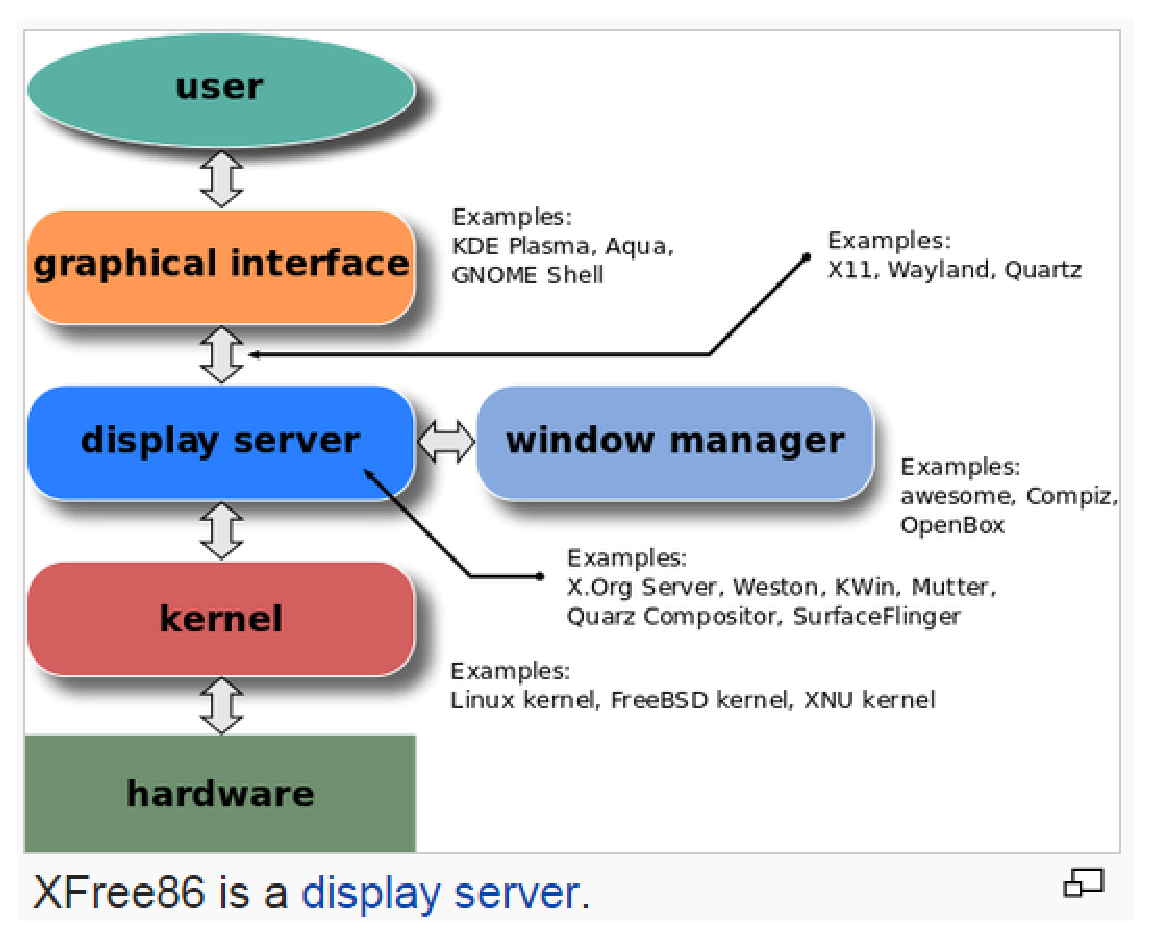
\includegraphics[height=5cm,
    angle=0]{./images/XFree86.eps}}
\caption{XFree86 is a display server}
\label{fig:XFree86}
\end{figure}

\begin{framed}
  XFree86 is the open-source implementation of X11-based desktop
  infrastructure in the form of client-server that provide a
  connection between the window manager (KDE, GNOME...) with the
  hardware (mouse, keyboard, video
  display...)\footnote{\url{http://www.xfree86.org/}}. 
\end{framed}

An early project to integrate accelerated 3D into XFree86 3.3 was called Utah
GLX. Another effort to develop hardware driver for the XFree86 was carried out
by Precision Insight, Inc. (PI) through contracts with various IHVs and ISVs. PI
began the development of the OpenGL DRI ({\bf Direct Rendering Infrastructure})
- the foundation for 3D graphics support on Linux.
The primitive architecture of Utah GLX makes it slower than the DRI but it is
much simpler to implement and is also easier to write drivers for.
\url{http://dri.freedesktop.org/wiki/UtahGLX/} 

The DRI was designed to be flexible in order to accomodate a variety of hardware
architectures. Since the hardware designs are changing and growing more
sophisticated the DRI will also evolve to accomodate these changes.

As of mid-2000 the DRI has been incorporated into XFree86 4.0 and at least five
distinct hardware device drivers have been developed. XFree86 4.0 introduced a
new device driver interface called XAA which should allow XFree86 drivers to be
backward compatible with future versions of the Xserver,
Fig.\ref{fig:XServer_rendering}(1).


The 3D DRI driver essentially converts OpenGL command sequences
into hardware commands. It then uses the kernel module to transmit the commands
to the hardware. It implements the entire OpenGL rendering pipeline
(Sect.\ref{sec:OpenGL}), as much of it as possible in the user space
while the kernel module does whatever is needed in kernel space.
3D DRI drivers usually reside in the 
\begin{verbatim}
/usr/X11R6/lib/modules/dri/
\end{verbatim} 
directory (or specified via \verb!LIBGL_DRIVERS_PATH! environment variable) with
names of the form \verb!device_dri.so.!

In POSIX-based system, the configuration file of XFree86 is in
\begin{verbatim}
/etc/X11/XF86Config
/etc/X11/XF86Config-4
\end{verbatim}
that includes variables about the screen (monitor), keyboard and graphics card.
 
% X.org is the dominant project now with X.org Server is the implementation of 
% X11.

\subsection{DirectFB}
\label{sec:DirectFB}

DirectFB ({\bf Direct FrameBuffer}) functions like X Window System
(Sect.\ref{sec:X11}). However, DirectFB was designed for embedded systems, which
have smaller memory footprint, Fig.\ref{fig:DirectFB}.

\begin{figure}[hbt]
  \centerline{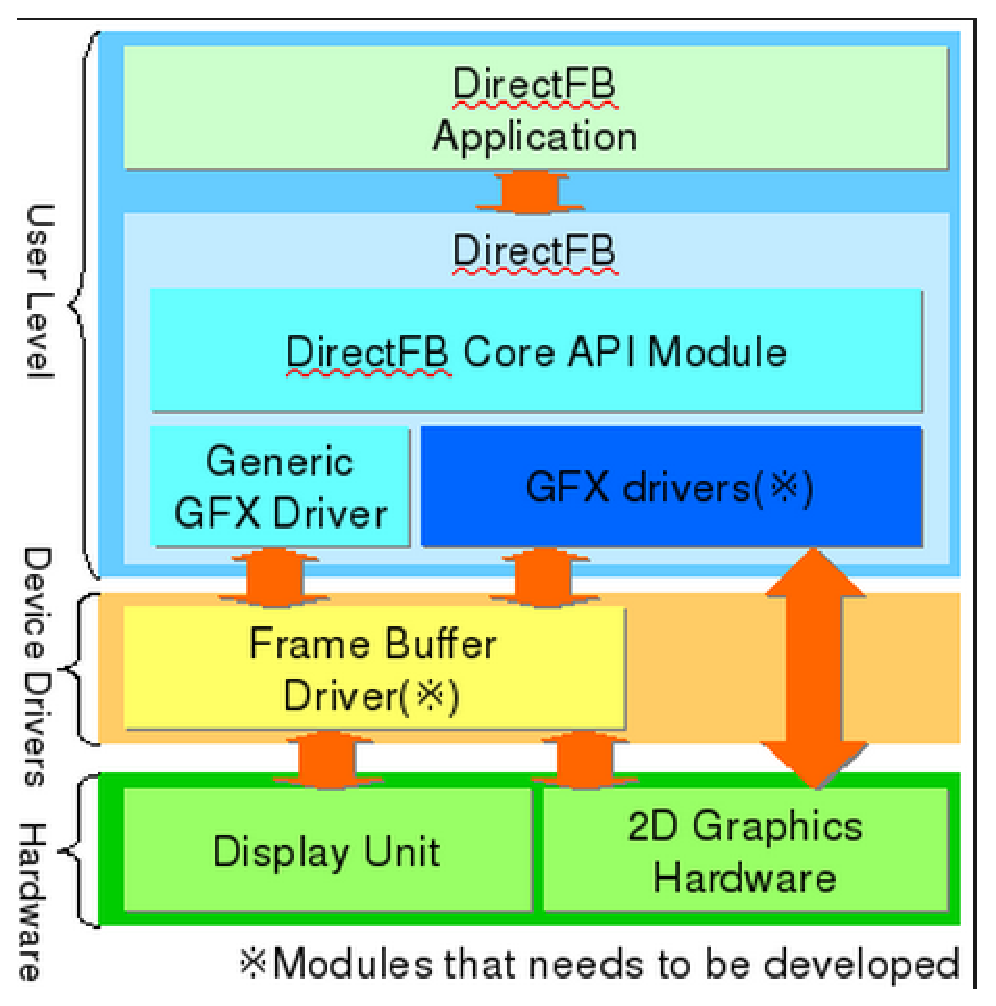
\includegraphics[height=5cm,
    angle=0]{./images/DirectFB.eps}}
\caption{DirectFB}
\label{fig:DirectFB}
\end{figure}


\url{http://stackoverflow.com/questions/3327767/why-is-directfb-not-more-widely-used-in-gnu-linux-are-there-crippling-limitatio}

\subsection{Emulate tools: Xnest, Xephyr}

An X client may emulate an X server by providing a display service
to other X clients. This technique is called {\bf X nesting}. Open-source tools
are \verb!Xnest! and \verb!Xephyr!.

\subsection{Xgl X server}
\label{sec:Xgl}

Xgl is the new XServer architecture layered on top of OpenGL.
It uses two variants of backend implementation, Fig.\ref{fig:Xglx_Xegl} 
to takes advantage of the modern GPUs using OpenGL (Sect.\ref{sec:OpenGL}).
\begin{itemize}
  \item {\bf Xglx}: requires an existing X server and uses GLX
  (Sect.\ref{sec:GLX}) to create an OpenGL window.
  
Xgl must be used in combination with a compositor/window manager to expose all
of its capabilities. Compiz is the compositor utility that was developed in
conjunction with Xgl. Glitz is the key component of the Xgl X server, as it
supports Compiz.

  \item {\bf Xegl}
\end{itemize}
\url{https://tr.opensuse.org/Xgl}

\begin{figure}[hbt]
  \centerline{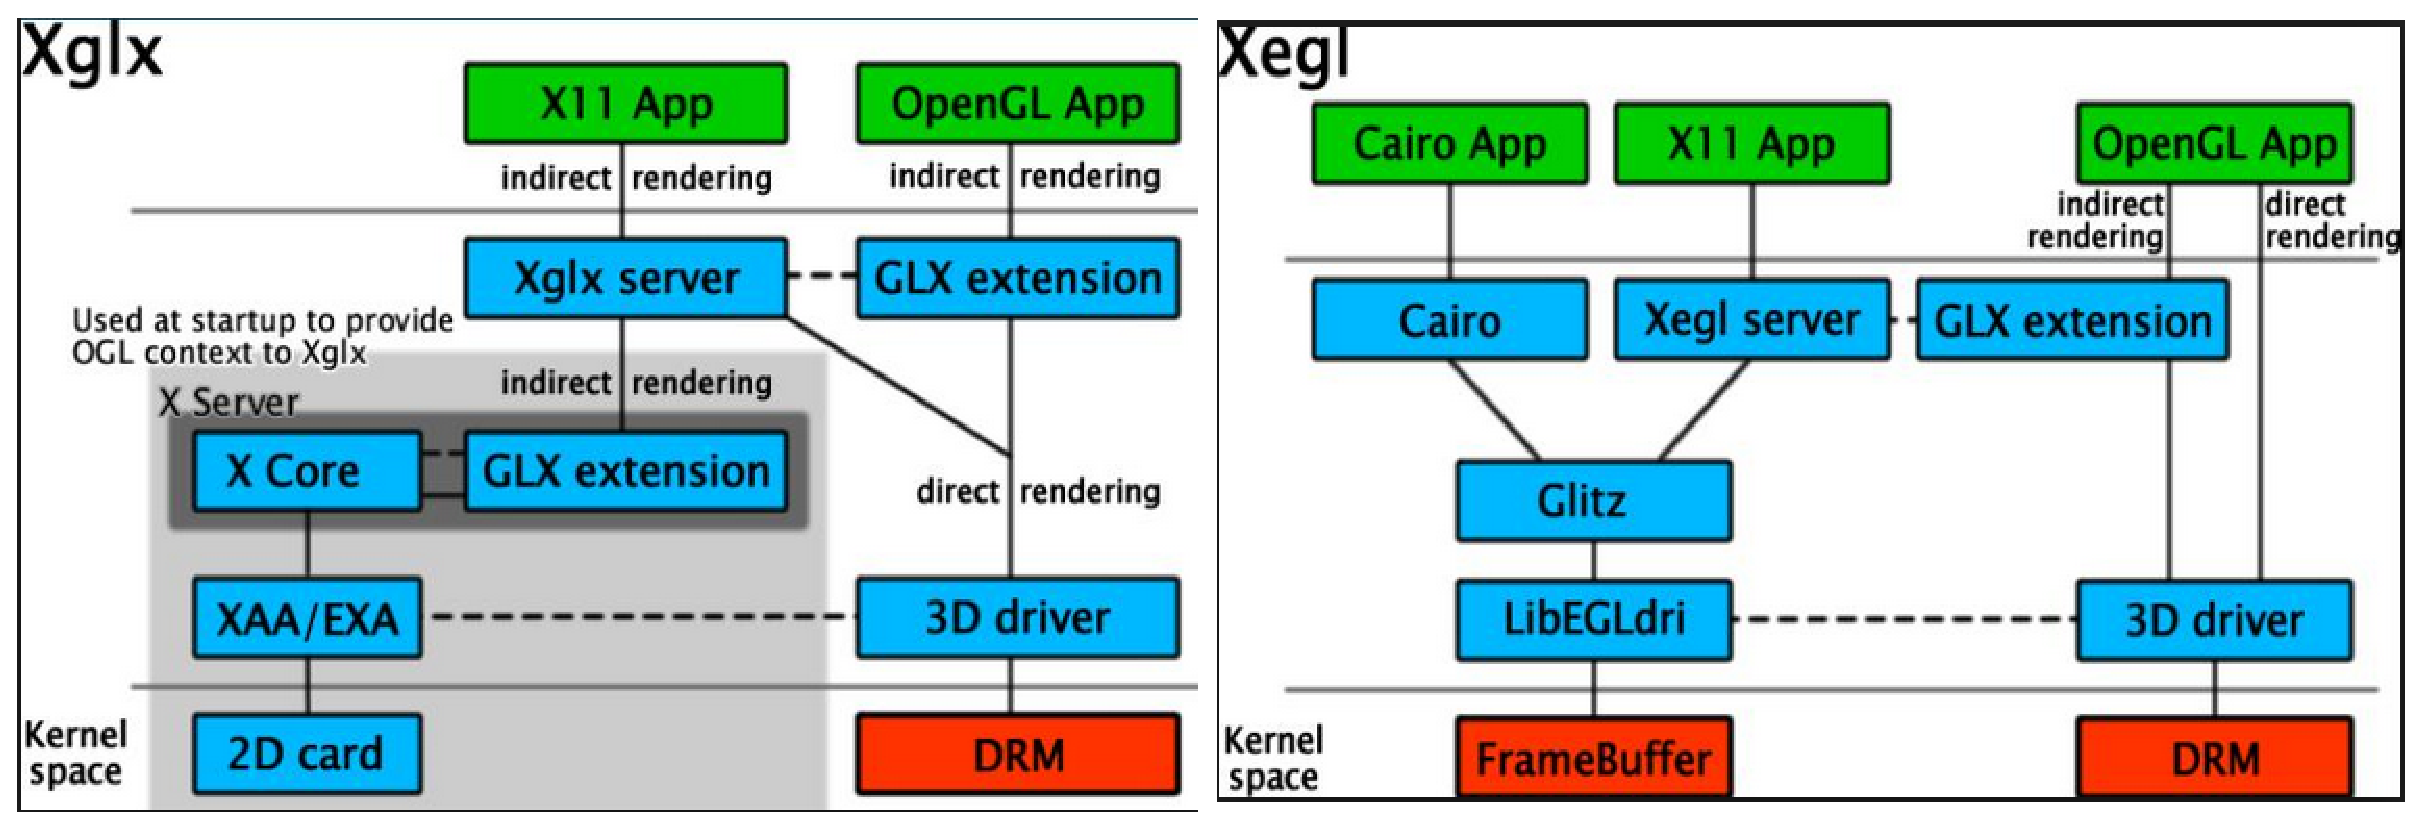
\includegraphics[height=5cm,
    angle=0]{./images/Xglx_Xegl.eps}}
\caption{(A) Xglx server was implemented on top of X Server to provide direct
rendering. (B) Xegl}
\label{fig:Xglx_Xegl}
%http://blog.csdn.net/shallon_luo/article/details/4904769
\end{figure}

%Xgl was first released in 2006, but then was removed in favour of AIGLX.



\section{-- X11's display to Windows}

Suppose you have a headless Linux machine, and you want to display the GUI from
that Linux machine (running X11 server -
Sect.\ref{sec:X-server-implementation}) on a Windows machine. There are several
options:

\begin{enumerate}
  \item VcXsrv - Sect.\ref{sec:VcXsrv} - work best on Windows 64-bit O/S.
  
  
  \item Cygwin/X - Sect.\ref{sec:Cygwin/X}
  \item Xming - Sect.\ref{sec:Xming}
  \item WeirdX - Sect.\ref{sec:WeirdX}
\end{enumerate}

\subsection{VcXsrv}
\label{sec:VcXsrv}

To run Remote X Linux Apps from Windows, for 64-bit Windows 7 and above, you
should consider using VcXsrv Windows X Server.
\begin{itemize}
  \item  MS Windows X11 server based on the Xorg git sources (like xming or
  cygwin's xwin)
  \item actively updated
  \item compiled with VC++ 2012 Express Edition, not 'mingw' making it very MS
  Windows stable.
  
\end{itemize}

\url{https://bbs.nextthing.co/t/need-an-x11-server-for-win7-or-above-vcxsrv-is-based-on-xorg/2882}

\url{https://sourceforge.net/projects/vcxsrv/files/latest/download}


\subsection{MobaXTerm}
\label{sec:MobaxTerm}

MobaXTerm is "sort of" free... it carries its own SSH client and X Display
Server (i.e. client). MobaXTerm is based on Cygwin.

Run MobaxTerm, open Settings/Configuratin, select X11 tab
\begin{verbatim}
Xorg version:
   MobaX
   Cygwin_1.14.5
   Cygwin_1.16.3
   
OpenGL acceleration: Software / Hardware
  --> select Hardware
  
Clipboard: 
  --> select enabled
  
\end{verbatim}


\subsection{Cygwin/X}
\label{sec:Cygwin/X}

Cygwin/X is an implementation of X server on Windows platform. It enables
running a remote/local X11 applications in Windows.

\subsection{Xming}
\label{sec:Xming}

Like Cygwin/X (Sect.\ref{sec:Cygwin/X}), Xming is another implementation of X
server on Windows platform. It is simple and easier to install though less
configurable than other popular free choices like Cygwin/X.

\subsection{WeirdX}
\label{sec:WeirdX}

WeirdX is a pure Java implementation of X Window System server that of course
can run on Windows O/S.
\url{http://sourceforge.net/projects/weirdx/}


\section{ * X11's X client library stack}
\label{sec:X-client-implementation}

An X11 client application is a GUI application, that calls to X11-based APIs
for graphics purpose. There are different libraries that implement X11-based
network protocol APIs. NOTE: The client program can run locally or remotely. 
\begin{itemize}
  \item {\bf Xlib} (Sect.\ref{sec:Xlib}) or 
  
  \item {\bf XCB} (Sect.\ref{sec:XCB})
\end{itemize}
At the bottom level of the X client library stack are Xlib and XCB, two helper
libraries (really sets of libraries) that provide API for talking to the X server. 

Xlib and XCB only provides a set of APIs for the client to tell the server-side
how to render the UI. However, looks-and-feel of the UI components are
implemented by many widget toolkits which built on top of Xlib or XCB,
Fig.\ref{fig:widget_library_system}. So, most likely, you don't have to work
directly with Xlib or XCB, just focus on using Widget toolkits
(Sect.\ref{sec:widget-toolkits-list}).

\begin{mdframed}

How the GUI component looks like (i.e. the visual styling) is not determined by X Window
System. Thus, we can develop the user interface to run on the command-line using
X's graphical capabilities. Also, X provides no native support for audio. 
If we need visual styling, please use Widget toolkits which is a higher level
APIs that enclose calls to these X11 client libraries.
Sparingly, a GUI application may find themselves needing to make calls to the
raw underlying X11 libraries for operations not supported by toolkits.

\end{mdframed}

\subsection{XLib (libX11)}
\label{sec:Xlib}
\label{sec:libX11}

In 1985, {\bf Xlib} library is a X client library, i.e. it provides APIs to
allow the client program to interact with X server easier, by hiding the fact
that calls result in protocol requests to a server. 
\begin{itemize}
  
  \item   Calls that don't require a response from the X server are queued in a
  buffer to be sent as a batch of requests to the server.
  
  \item Those that require a response flush all the buffered requests and then
  block until the response is received.
  
\end{itemize}
Using Xlib is not easy, the thus XCB was developed (Sect.\ref{sec:XCB}).

\begin{mdframed}

Xlib's mix of synchronous and asynchronous behaviors causes some problems.
Xlib's behaviour is often confusing to new programmers. Calls appear to work
sometimes and not others, because it is not obvious which calls implicitly flush
the buffer. The asynchronous nature of many calls makes it difficult to debug
problems. When an error is reported, the stack trace shows the call that was
being made when the error was received and processed, often many calls after the
one that caused the error. Finally, Xlib's synchronous calls incur avoidable
round-trip latency. This latency has a notable effect on application
performance; in particular, startup times are often greatly increased.
\url{https://www.x.org/wiki/guide/xlib-and-xcb/}
\end{mdframed}

Each new extension to the X11 protocol (Sect.\ref{sec:X11}) adds requests that
clients can make to the X server.
Thus, Xlib is aka {\it libX11 for X Window System version 11}. Xlib is written
in C, so Xlib is aka {\it C Library X Interface}. To link to this library, we
pass the following option to the compiler
\begin{verbatim}
-lX11
\end{verbatim}

The programmer needs not know details about X Window System protocol when using
Xlib.
\begin{itemize}
  \item Xlib only provides the API to interact with the X11 Server but does not
  provide any API to implement different GUI components, e.g. buttons or menus.

header file:
\begin{verbatim}
#include <stdio.h>
#include <stdlib.h>
#include <X11/Xlib.h>
#include <X11/Xutil.h>
#include <X11/Xos.h>
#include <X11/Xatom.h>
#include <X11/keysym.h>
\end{verbatim}

  \item APIs provided by Xlib can (1) opening a new window, (2) draw a line, (3)
  write text at a given location in a given window.

As the rendering is taken care by the server-side, Xlib library has no need to
know about the look-and-feel of the UI. 

\end{itemize}

Example: the server is a computer with two video cards, each card can connect to
one or more monitor.  a "display" is a collection of "screens" attached to a
single display device (e.g. a graphics card).

There are 4 important elements in Xlib
\begin{verbatim}
	Display *dis;
	int screen;
	Window win;
	GC gc;
\end{verbatim}


Example: Xlib APIs
\begin{itemize}
  \item XOpenDisplay(), XCloseDisplay

\textcolor{red}{First, connect to the screen which requires the information
about server name and display index (e.g. the graphics card)}
\url{http://tronche.com/gui/x/xlib/display/opening.html}
\begin{verbatim}
Display *XOpenDisplay(display_name)
      char *display_name;
\end{verbatim}  
input can be either a string in the format \verb!hostname:number.screen_number!
\begin{verbatim}
hostname = the machine on which the GUI is displayed
number   = the index of graphic card at 'hostname' (i.e. the display 0 or 1 or
            ???)

screen_number = the index of the screen connected to the
               selected graphics card
               on machine 'hostname'
\end{verbatim}
or NULL (use the string information from DISPLAY environment
variable) 
\url{http://www.pyglet.org/doc/programming_guide/displays_screens_configs_and_contexts.html}

  \item XCreateWindow(), XCreateSimpleWindow()
  
\textcolor{red}{Once the screen is connected, we can request to create a
window}, which returns an {\bf identifiers}, i.e. the client communicate with
the server and ask the server to do specific work for the window of the
given identifier.
\url{http://tronche.com/gui/x/xlib/window/XCreateWindow.html}

% NOTE: XCreateSimpleWindow() requires the screen already connected as it is an
% argument to the function.
\begin{verbatim}
dis = XOpenDisplay(NULL);
win = XCreateSimpleWindow(dis, RootWindow(dis, 0), 1, 1, 500, 500, \
0, BlackPixel (dis, 0), BlackPixel(dis, 0));
\end{verbatim}

  \item XCreateGC()

Graphics context (GC) has a lot to do with how things are displayed/drawn in the
window. Different masks can be set, etc. and you can get pretty funky with it.
\begin{verbatim}
/* create the Graphics Context */
gc=XCreateGC(dis, win, 0,0);    

/* here is another routine to set the foreground and background
	   colors _currently_ in use in the window.
	*/
XSetBackground(dis,gc,white);
XSetForeground(dis,gc,black);
\end{verbatim}
\url{http://math.msu.su/~vvb/2course/Borisenko/CppProjects/GWindow/xintro.html}

  \item XMapWindow()
  
\textcolor{red}{map the created window to the screen}

  \item XGetWindowProperty()
  
  \item XSelectInput()
  
Tell the X Server what kind of event that the program want to process
\begin{verbatim}
XSelectInput (dis, win, ExposureMask | KeyPressMask | ButtonPressMask);
\end{verbatim} 
NOTE: In the event-loop, we will check for the occuring of these event using
operation on the event queue

  \item operation on event queue: XNextEvent(), XPeekEvent(), 
  
XPeekEvent() function returns the first event from the event queue, but
it does not remove the event from the queue
  
Events in X are things like the mouse buttons being clicked, or the keys on the
keyboard being pressed. The events can either be KeyPress or KeyRelease for
keyboard control devices.
 When the window is resized the application is sent a ConfigureNotify event.
When the window is below another window and is raised it is sent an Expose
event, which would usually redraw the application. When the window is initially
created an Expose event is sent.


  \item operations on local dataa: XCreateImage(), XSaveContext(),
  XParseGeometry()
\end{itemize}
  
The main type of data in Xlib are \verb!Display! structure and types of
{\it identifiers} (e.g. \verb!Windows!, \verb!Pixmap!, \verb!Font!,
\verb!Colormap!). Identifiers are 32-bit integers.
\begin{itemize}
  \item Windows, colormaps, etc. are managed by the server, which means that the
  data about their actual implementation is all stored in the server. 
  
  \item The client operates on these objects by using their identifiers. The
  client cannot directly operate on an object, but can only request the server
  to perform the operation specifying the identifier of the object.
\end{itemize}
Most Xlib functions have a Display structure as an argument because they either
operate on the channel or are relative to a specific channel. 

\textcolor{red}{To be able to catch different events, an infinite loop (event
loop) is the common approach in GUI program}. This is called event-driven
application (Sect.\ref{sec:event_driven_app})
\begin{verbatim}

while (1)  {
  XNextEvent(dis, &report);
  switch  (report.type) {
    case Expose:   
      fprintf(stdout, "I have been exposed.\n");
/*A local program function to redraw the window should be called.*/
    break;
    }
  
  
    if (event.type==KeyPress&&
		    XLookupString(&event.xkey,text,255,&key,0)==1) {
		/* use the XLookupString routine to convert the invent
		   KeyPress data into regular text.  Weird but necessary...
		*/
			if (text[0]=='q') {
				close_x();
			}
			printf("You pressed the %c key!\n",text[0]);
		}  
}

\end{verbatim}

\textcolor{red}{Finally, implement the function to free memory once the program
exit}
\begin{verbatim}
void close_x() {
/* it is good programming practice to return system resources to the 
   system...
*/
	XFreeGC(dis, gc);
	XDestroyWindow(dis,win);
	XCloseDisplay(dis);	
	exit(1);				
}
\end{verbatim}


Example: A client 'creates' a window by requesting that the server create
a window. This is done via a call to an Xlib function that returns an identifier for the
window, that is, a number. The client then use this identifier for requesting
other operations on the same window to the server.

The Xlib functions that send requests to the server usually do not send these
requests immediately but store them in a buffer, called the
\textcolor{red}{\bf request buffer}. 
The request buffer can contain all kinds of requests to the server, not only
those having a visible effect on the screen. 
The request buffer is guaranteed to be flushed (i.e., all requests done so far
are sent to the server) after a call to the functions \verb!XSync! or
\verb!XFlush!.

NOTE: The X Server returns \verb!events! to the Xlib which stores them in a
queue. While the X server sends events asynchronously, applications using the
Xlib library are required to explicitly call Xlib functions for accessing the
events in the queue.
\url{http://en.wikipedia.org/wiki/Xlib}

Example:
\begin{verbatim}
#include <X11/Xlib.h>

int main(void)
{
    Display *display;
    Window window;
    XEvent event;
    int s; // identifier
    
     /* open connection with the server */
    display = XOpenDisplay(NULL);
    
    s = DefaultScreen(display);
    
    /* create window */
    window = XCreateSimpleWindow(display, RootWindow(display, s), 10, 10, 200, 200, 1,
                           BlackPixel(display, s), WhitePixel(display, s));
 
    /* select kind of events we are interested in */
    XSelectInput(display, window, ExposureMask | KeyPressMask);
 
    /* map (show) the window */
    XMapWindow(display, window);
    
    
    /* event loop */
    for (;;)
    {
        XNextEvent(display, &event);
 
        /* draw or redraw the window */
        if (event.type == Expose)
        {
            XFillRectangle(display, window, DefaultGC(display, s), 20, 20, 10, 10);
            XDrawString(display, window, DefaultGC(display, s), 50, 50, msg, strlen(msg));
        }
        /* exit on key press */
        if (event.type == KeyPress)
            break;
    }
 
    /* close connection to server */
    XCloseDisplay(display);

   return 0;
}
\end{verbatim}

\subsection{XCB (libxcb)}
\label{sec:XCB}
\label{sec:libxcb}

XCB (X protocol C-language Binding) - aims to replace Xlib (libX11).

XCB makes the client-server nature of the protocol explicit in its design. The
client is in charge of deciding when to flush the request buffer, when to read
results and when to wait for the server to respond.



\subsection{Xlib/XCB}

Xlib/XCB is the modern choice which implement Xlib on top of XCB library, i.e.
rebuild libX11 as a layer on top of libxcb. 

One can use Xlib to open the display and pass the Display pointer it returns to
existing code, toolkits, and libraries. To call an XCB function, one can convert
the Display pointer to an \verb!xcb_connection_t! pointer for the same
connection.
This enables calling into Xlib and XCB from the same application.
Xlib and XCB share the same X server connection and pass control of it back and
forth. That option was introduced in libX11 1.2, and is now always present (no
longer optional) since the 2010 release of libX11 1.4.




\section{Mir}
\label{sec:Mir}

{\bf Mir} is a  display server (Sect.\ref{sec:display-server}) for the Linux
operating system that is under development by Canonical Ltd since 2013.

The goal to have Mir is to have lower overhead in the display pipeline, more
seamless transitions between display modes during the boot process, richer input
handling that will make it easier to support things like touchscreen gestures,
more seamless support for systems with switchable graphics hardware (like
laptops that can dynamically shift between using embedded and discrete
graphics), and better application interchange (which will help improve things
like the clipboard and drag-and-drop).

\begin{enumerate}
  \item Unity 8 has native support for Mir
  
  \item 
\end{enumerate}
The compatibility layer for X, XMir, is based on XWayland.



\section{History of 2D graphics library in Windows}
\label{sec:2D-graphics-Windows}

\subsection{Port X-Windows System to Windows}

There are different implementation that allows displaying the UI of a
programming running on a 'remote' X-Windows system on Windows.

{\bf X-Win32} a proprietary implementation of the X Window System for Microsoft
Windows, based on X11R7.4. It allows a remote Unix program to display on Windows
local machine. \url{http://en.wikipedia.org/wiki/X-Win32}

{\bf Cygwin/X} is a free alternative to provide a similar featuer as X-Win32,
and is part of the Cygwin project (Sect.\ref{sec:Cygwin/X}).
Cygwin/X was originally based on XFree86 (Sect.\ref{sec:XFree86}), but
has been switched to the X.Org Server since the discontinuing of XFree86
project.
\begin{itemize}
  \item provide an X Server environment to run GUI application from Cygwin
  \item provide an X Server environment to run GUI application from a remote
  Linux machine. Protocols it supports: XDM, SSH tunneling.
\end{itemize}

{\bf Xming Server} a proprietary implementation based on Cygwin/X and X.Org
Server. Protocols for remote connection: SSH X11 forwarding, PuTTYs

{\bf Xwin} - a strip-down version of Cygwin/X, just for running X Server in
Windows. \url{http://wiki.dennyhalim.com/xwin}

\subsection{GDI (16-bit): use DC (device context) objects}
\label{sec:GDI}
\label{sec:DC-device-context}

To provide the UI to a program running on Windows, GDI was introduced since the
first version of Windows. GDI is a C library and is 16-bit library. On 32-bit
platform, it is replaced by Win3 GDI (Sect.\ref{sec:Win32GDI}).

The goal of developing GDI is to provide a device-independent API, i.e.
a program written using the GDI will work on all graphics and printer hardware,
provided suitable Windows GDI drivers for the hardware are installed on the
system. 

A common device-independent approach is to write data (graphics (bitmaps)) to a
logical graphics {\bf device context} (DC), but not to the physical framebuffer
on the hardware directly.
\textcolor{red}{The major limitation of the GDI DCs was that they were {\bf
write-only}}. Data, once written, could not be retrieved.
This was because the contents of the DC was device dependent, and data read from
it would make no sense to the programmer.

A {\bf bitmap} is the in-memory representation of the picture to be drawn on the
drawing surface of the DC. GDI also has a number of functions that can copy
areas from the drawing surface of one DC to another, so bitmaps then are a
useful way to store images in memory that will later be copied to the display
(or other devices).

The DC is then translated by the GDI and the device drivers to suit the target
hardware device and is written to its physical frame buffer in an appropriate
manner
\begin{itemize}
  
  \item A {\bf Device Context} (DC) is a handle to a drawing surface on some
  device - Device Contexts can typically be obtained for the display device (the
  entire screen), printers and plotters.
  
Most commonly worked with are {\bf window DC} (a display DC that merely
represents the area of a single window) and a {\bf memory DC} that represents a
bitmap as a device.

  \item For a given DC, a number of tools that can be used to act on the
  associated drawing surface: Pens, brushes, fonts, etc.
  
In the case of memory DC, a number of preset pens are provided, and more can be
created on the fly as needed.
\end{itemize}

%GDI is too slow for animation, as it cannot access hardware directly.
In order to do animation using the GDI DC, all of the animation frames needed to
be manipulated in system memory and then each frame needed to be copied into a
GDI DC for display on the graphics device. This was a very slow process.

\url{http://www.codeproject.com/Articles/356/Bitmap-Basics-A-GDI-tutorial}

\subsection{DCI (Device Control Interface)}
\label{sec:DCI}

\url{http://stason.org/TULARC/pc/video-faq/54-What-is-DCI.html#.VOWN_fnF_Xo}

Unlike GDI, which doesn't write data directly to hardware graphics bufer, DCI
was developed to enable that feature, i.e. faster. The goal was to support
video games that require fast rendering.
DCI is replaced by DirectDraw (Sect.\ref{sec:DirectDraw}).

DCI stands for "Device Control Interface." It's an Intel/Microsoft standard, and
exists primarily as a way for Windows 3.1 to exploit the video acceleration
features of a graphics card, and/or to provide fast video when needed. 

A DCI driver exists at the same software layer as the GDI.
Thus, support for DCI features doesn't need to be in hardware -- a graphics card
vendor could provide a DCI driver that allowed Windows 3.1 apps to speak DCI,
but the graphics card could be performing the DCI functions with a software
driver.

Among DCI's capabilities are the ability to {\it write directly to the frame
buffer} (helpful for high-speed games) and the ability to provide for on-board
hardware acceleration of video scaling (i.e. stretching a video window to a
larger size) and color space conversion (converting the YUV format color
information in a video file to the RGB format that a typical graphics card
RAMDAC expects).


\subsection{WinG (Win 3.x): WinGDC}
\label{sec:WinG}

As the original GDI was designed with static image in mind, it is not suited for
video (games). WinG APIs was developed as a quick-fix to GDI API.
WinG APIs was used in Windows 3.x, and until Windows 95, Windows 98 and Windows
NT 4.0; and stopped since Windows 98 Second Edition, Windows 2000, due to the 
inception of DirectX (Sect.\ref{sec:DirectX}).

% NOTE: DC in GDI is write-only. 
% 
Using the DC concept similar to GDI (Sect.\ref{sec:GDI}), WinG introduced a new
type of device context called {\bf WinGDC} that uses DCI (Sect.\ref{sec:DCI})
and thus allowed programmers to both read and write to it directly using DIB
(device-independent bitmap) with \verb!wingdib.drv! driver.

This meant that fast graphics algorithms could be written to allow fast
scrolling, overdraw, dirty rectangles, double buffering, and other animation
techniques.
WinG also provided much better performance when blitting graphics data to
physical graphics device memory.

WinG would also perform a graphics hardware/driver profiling test on the first
execution of the program in order to determine the best way to manipulate the
graphics hardware.
Once WinG had determined the fastest calls that did not cause graphics
corruption, a profile would be saved so that the test would not need to be
performed again.


\subsection{Win32 GDI (32-bit)}
\label{sec:Win32GDI}

In Windows, Win32 GDI (Graphics Device Interface) is the GDI library for graphics
model from Windows 95 and is supported on all 32-bit Windows (Win32) platforms.
When we say Win32, it means Win32 GDI. Win32 GDI is still a C library. 
A better replacement is DirectWrite (Sect.\ref{sec:DirectWrite}). 

\begin{mdframed}

GDI a low-level library and is responsible for tasks such as drawing lines and
curves, rendering fonts and handling palettes.
GDI is NOT responsible for drawing windows, menus, etc. These tasks are served
for APIs in \verb!user32.dll! libraries.

Thus, GDI is relatively hard to use for advanced animation, and lacks a notion
for synchronizing with individual video frames in the video card, lacks hardware
rasterization for 3D, etc.
\end{mdframed}

%A better replacement is OpenGL and DirectX.


\subsection{GDI+ (32-bit, C++): Windows XP}
\label{sec:GDI+}

GDI+ is C++ library to complement GDI C-based library since Windows XP.
GDI/GDI+ is replaced by Direct2D (Sect.\ref{sec:Direct2D})

GDI+ is an improvement on GDI with features not readily available
in GDI such as 
\begin{enumerate}
  \item gradient brushes, 
  
  \item alpha blending, and 

  \item GDI+ uses  ARGB values to represent color.

 \item anti-aliased 2D graphics, 
 
 \item floating point coordinates,

  \item gradient shading, 
  
  \item more complex path management, 
  
  \item more image format support: intrinsic support for modern graphics-file
  formats like JPEG and PNG, and support for composition of affine
  transformations in the 2D view pipeline.
 
\end{enumerate}
\url{http://stackoverflow.com/questions/4551224/what-is-the-difference-between-gdi-and-gdi}

NOTE: GDI+ is nearly an order of magnitude slower than GDI, but that's not too
big of an issue on modern machines with more power than you could ever want. 
%This, too, is going to be supported for a very long time to come.

The Microsoft .NET class library provides a managed interface for GDI+ via the
\verb!System.Drawing! namespace.

GDI+ continues to rely on software rendering in Windows 7.

\subsection{GAPIDraw (Graphics API - Windows Mobile)}
\label{sec:GAPI}

The Graphics API (GAPI) was a technology that allow  creation of
high-performance graphical applications across a variety of handheld hardware
configurations, including Palm, Symbian and Windows Mobile devices.
GAPI means Game    Application    Programming    Interface    for    
Drawing, and was originally designed for game development.
\url{http://dl.acm.org/citation.cfm?id=1052388}

It borrows many features from DirectX.
GapiDraw API is a mix between a Frame-Buffer API (i.e. draw using CPU) and a 
Graphic  Hardware  API (i.e. draw using GPU). GAPI was replaced by DirectDraw
(Sect.\ref{sec:DirectDraw}) since Windows Mobile 5.0. No maintainance for
backward compatibility since Windows Mobile 6.5.

GABI contained functions that allowed an application to request all button press
messages, even the ones that were normally intercepted by the Windows Mobile
operating system. This function is
\begin{verbatim}
 GXOpenInput()
\end{verbatim}
 
GAPI is using a DRAM buffer, i.e. you cannot write directly in the raw frame
buffer with GAPI, rather GAPI GXBeginDraw will return you the address of a
176x220 memory buffer, which will be copied in the real display frame buffer
when you call GXEndDraw.
\url{http://www.modaco.com/topic/241988-gapi-on-the-motorola-q-what-developers-need-to-know/}

 
\subsection{DirectDraw (part of DirectX on Windows Mobile)}
\label{sec:DirectDraw}

DirectDraw is 2D API, supports hardware acceleration and was used since
Windows Mobile 5.0. NOTE: For 3D rendering, read Sect.\ref{sec:Direct3D}

DirectDraw was then merged into a new package of {\bf DirectX 8.0} called
{\bf DirectX graphics} to extend Direct3D with DirectDraw APIs.

The header files and DirectDraw library is no longer included in DirectX SDK
since June-2010. Since DirectX 9.0, it is recommended to use Direct3D
(Sect.\ref{sec:Direct3D}) as you can do everything you want from DirectDraw, as
well as get better hardware acceleration and be able to add traditional 3D
related features (texture mapping, etc).

\verb!AllKeys()! is the keyboard API function to use in place of GAPI keyboard
function. 

IMPORTANT: \verb!AllKeys! exists as long as GAPI and GAPI
\verb!Gx(Open/Close)Input()! keyboard function is just a wrapper to this
function.

\begin{verbatim}
 GXOpenInput() with AllKeys(TRUE).
 
 GXCloseInput() with AllKeys(FALSE).
\end{verbatim}

Syntax:
\begin{verbatim}
BOOL AllKeys(

     BOOL bAllKeys

);

Nonzero indicates success. Zero indicates failure. To get extended error
information, call GetLastError.
\end{verbatim}
If bAllKeys is set to TRUE, this function allows all keyboard events to be sent
to the application. (This includes the soft-key buttons and back button).

If it is set to FALSE, this function specifies standard keyboard event behavior.
Some events including soft-key buttons and the back button are not sent to the application.

Example:
\begin{verbatim}
// process checkbox

case IDC_ALL_KEYS_CHECK_BOX:

if (g_AllKeys == true)

    {

    // Allow the OS to intercept some button presses

     AllKeys(FALSE);

    g_AllKeys = false;

    // set button state

    SendMessage(hwndCtl,BM_SETCHECK, BST_UNCHECKED,0);

    }

else

    {

    // Do not allow os to intercept button presses

    AllKeys(TRUE);

    g_AllKeys = true;

    //set button state

    SendMessage(hwndCtl,BM_SETCHECK, BST_CHECKED,0);

    }
\end{verbatim}

\subsection{Direct2D}
\label{sec:Direct2D}


\subsection{Uniscribe (text rendering)}
\label{sec:Uniscribe}

Uniscribe provides services for rendering Unicode-encoded text, especially
complex text layout. The library is \verb!USP10.dll! and is used in Windows
2000, Windows CE 5.0.

Uniscribe is replaced by DirectWrite since Windows 7
(Sect.\ref{sec:DirectWrite}).

\url{http://en.wikipedia.org/wiki/Uniscribe}

\subsection{DirectWrite (text rendering)}
\label{sec:DirectWrite}

DirectWrite is a text layout and glyph rendering API.
DirectWrite is designed to replace Uniscribe (Sect.\ref{sec:Uniscribe}) for
screen-oriented rendering and was shipped with Windows 7, Windows Server 2008 R2, \ldots

DirectWrite is hardware-accelerated when running on top of Direct2D
(Sect.\ref{sec:Direct2D}), but can also use CPU.




\section{History of 2D graphics library in Mac OS/X}

Developers for Mac O/S decided not to use X11; but Quartz
(Sect.\ref{sec:Quartz}). The reason was that so many features they needed was
not available in X11, and they decided to implement a whole new windowing
system. 

Back then, X didn't have any kind of compositing model and Quartz was better.
In terms of current capabilities, Quartz and a recent version of X.org are
similar. The difference is that X.org has a cleaner separation of policy and
mechanism, and maintains backwards compatibility with applications dating back
to the mid 1980s
 

\subsection{QuickDraw: used on MacOS Classic systems}

 QuickDraw, found on the old MacOS Classic systems, was a very simple design.
One process mediated access to the display, allocating regions to other
processes, and the other processes drew into these directly.

The obvious disadvantage to this was that all processes had access to the frame
buffer, so could corrupt the display easily and synchronizing drawing between
applications was very difficult.

\subsection{Display PostScript: NeXT systems}

Processes on old NeXT systems sent PostScript programs to the display server,
which then ran them. This had its own problems, such as the fact that the
display server effectively needed to be a complex multitasking virtual machine
to prevent programs from taking over all of the display's time.



\subsection{Quartz}
\label{sec:Quartz}

The design of Quartz was simple.
Just as a filesystem virtualizes the disk by providing virtual disks (files) to
applications, Quartz virtualizes the screen by providing virtual frame buffers
(windows) to applications. This is the Quartz Compositor or simply the 'Window
Server,'. The window server provides a region of shared memory to clients for
drawing and then composites this into the frame buffer (on the GPU).
It's a little bit more complicated than that, because this buffer is now an
OpenGL texture and can be the result of rendering OpenGL graphics to the texture
or compositing other textures together.


In Mac OS, Quartz is the graphics model.
\begin{itemize}
  \item Quartz 2D: 2D text and graphics rendering library

Since Mac OS X 10.4, Quartz 2D Extreme, which allows Quartz 2D to use supported GPUs for rendering.
As of Mac OS X v10.5 Quartz 2D Extreme has been renamed to QuartzGL.

\url{http://en.wikipedia.org/wiki/Quartz_(graphics_layer)}
  
  \item Quartz compositor: the compositing engine
  (Sect.\ref{sec:compositing_engine}). 
  
  It is used by Quartz 2D, OpenGL, Core Image, QuickTime.
  
  Since Mac OS X 10.2, Quartz Compositor uses GPU directly to improve composition performance.
    
\end{itemize}

% \section{X Window System vs. Quartz vs. Win32 GDI}
% 
% X Window System is the implementation for client-server communication in Linux.




\section{History of 2D/3D graphics library}
\label{sec:3D_graphics-library}

CRT monitors were first used to display ASCII text. Then, they are
used for displaying lines and points which can be combined to form
more complicated geometric shapes. In 1970s and 1980s, there is a
science of creating algorithms for efficiently creating lines and
curves on the display. These first computer graphics are 2D, with libraries
implemented the algorithms that we have introduced in the earlier sections
(Sect.\ref{sec:2D-graphics-Windows}, Sect.\ref{sec:2D-graphics-Linux}).

Then, there is a demands of producing animation or a sequence of
images that they call {\it real-time} in response to some input
(keyboard, mouse, joystick...) which is largely used in computer
games. At it was only 2D graphics, and then 3D graphics was developed to provide a
more visual-realistic perspective to the graphics (image, video).

Since the X11 standard was much earlier, it has no 3D features (until some
efforts - Sect.\ref{sec:X11-3D}), so OpenGL has become the common way of
providing these. The OpenGL standard (Sect.\ref{sec:OpenGL}) is an API defining
an abstract 3D language (the other common API being Microsoft's Direct3D -
Sect.\ref{sec:Direct3D}).

\textcolor{red}{In Linux, the APIs for graphics handling is not part of the O/S
kernel}. Initially, in Linux, X Server directly managed the resources of GPU
(Sect.\ref{sec:XServer}) via the 2D driver inside X Server,
Fig.\ref{fig:XServer_rendering}(1). To enable OpenGL application running on X
Server, Utah GLX was implemented using GLX protocol (Sect.\ref{sec:GLX}),
Fig.\ref{fig:XServer_rendering}(2).

\begin{figure}[hbt]
  \centerline{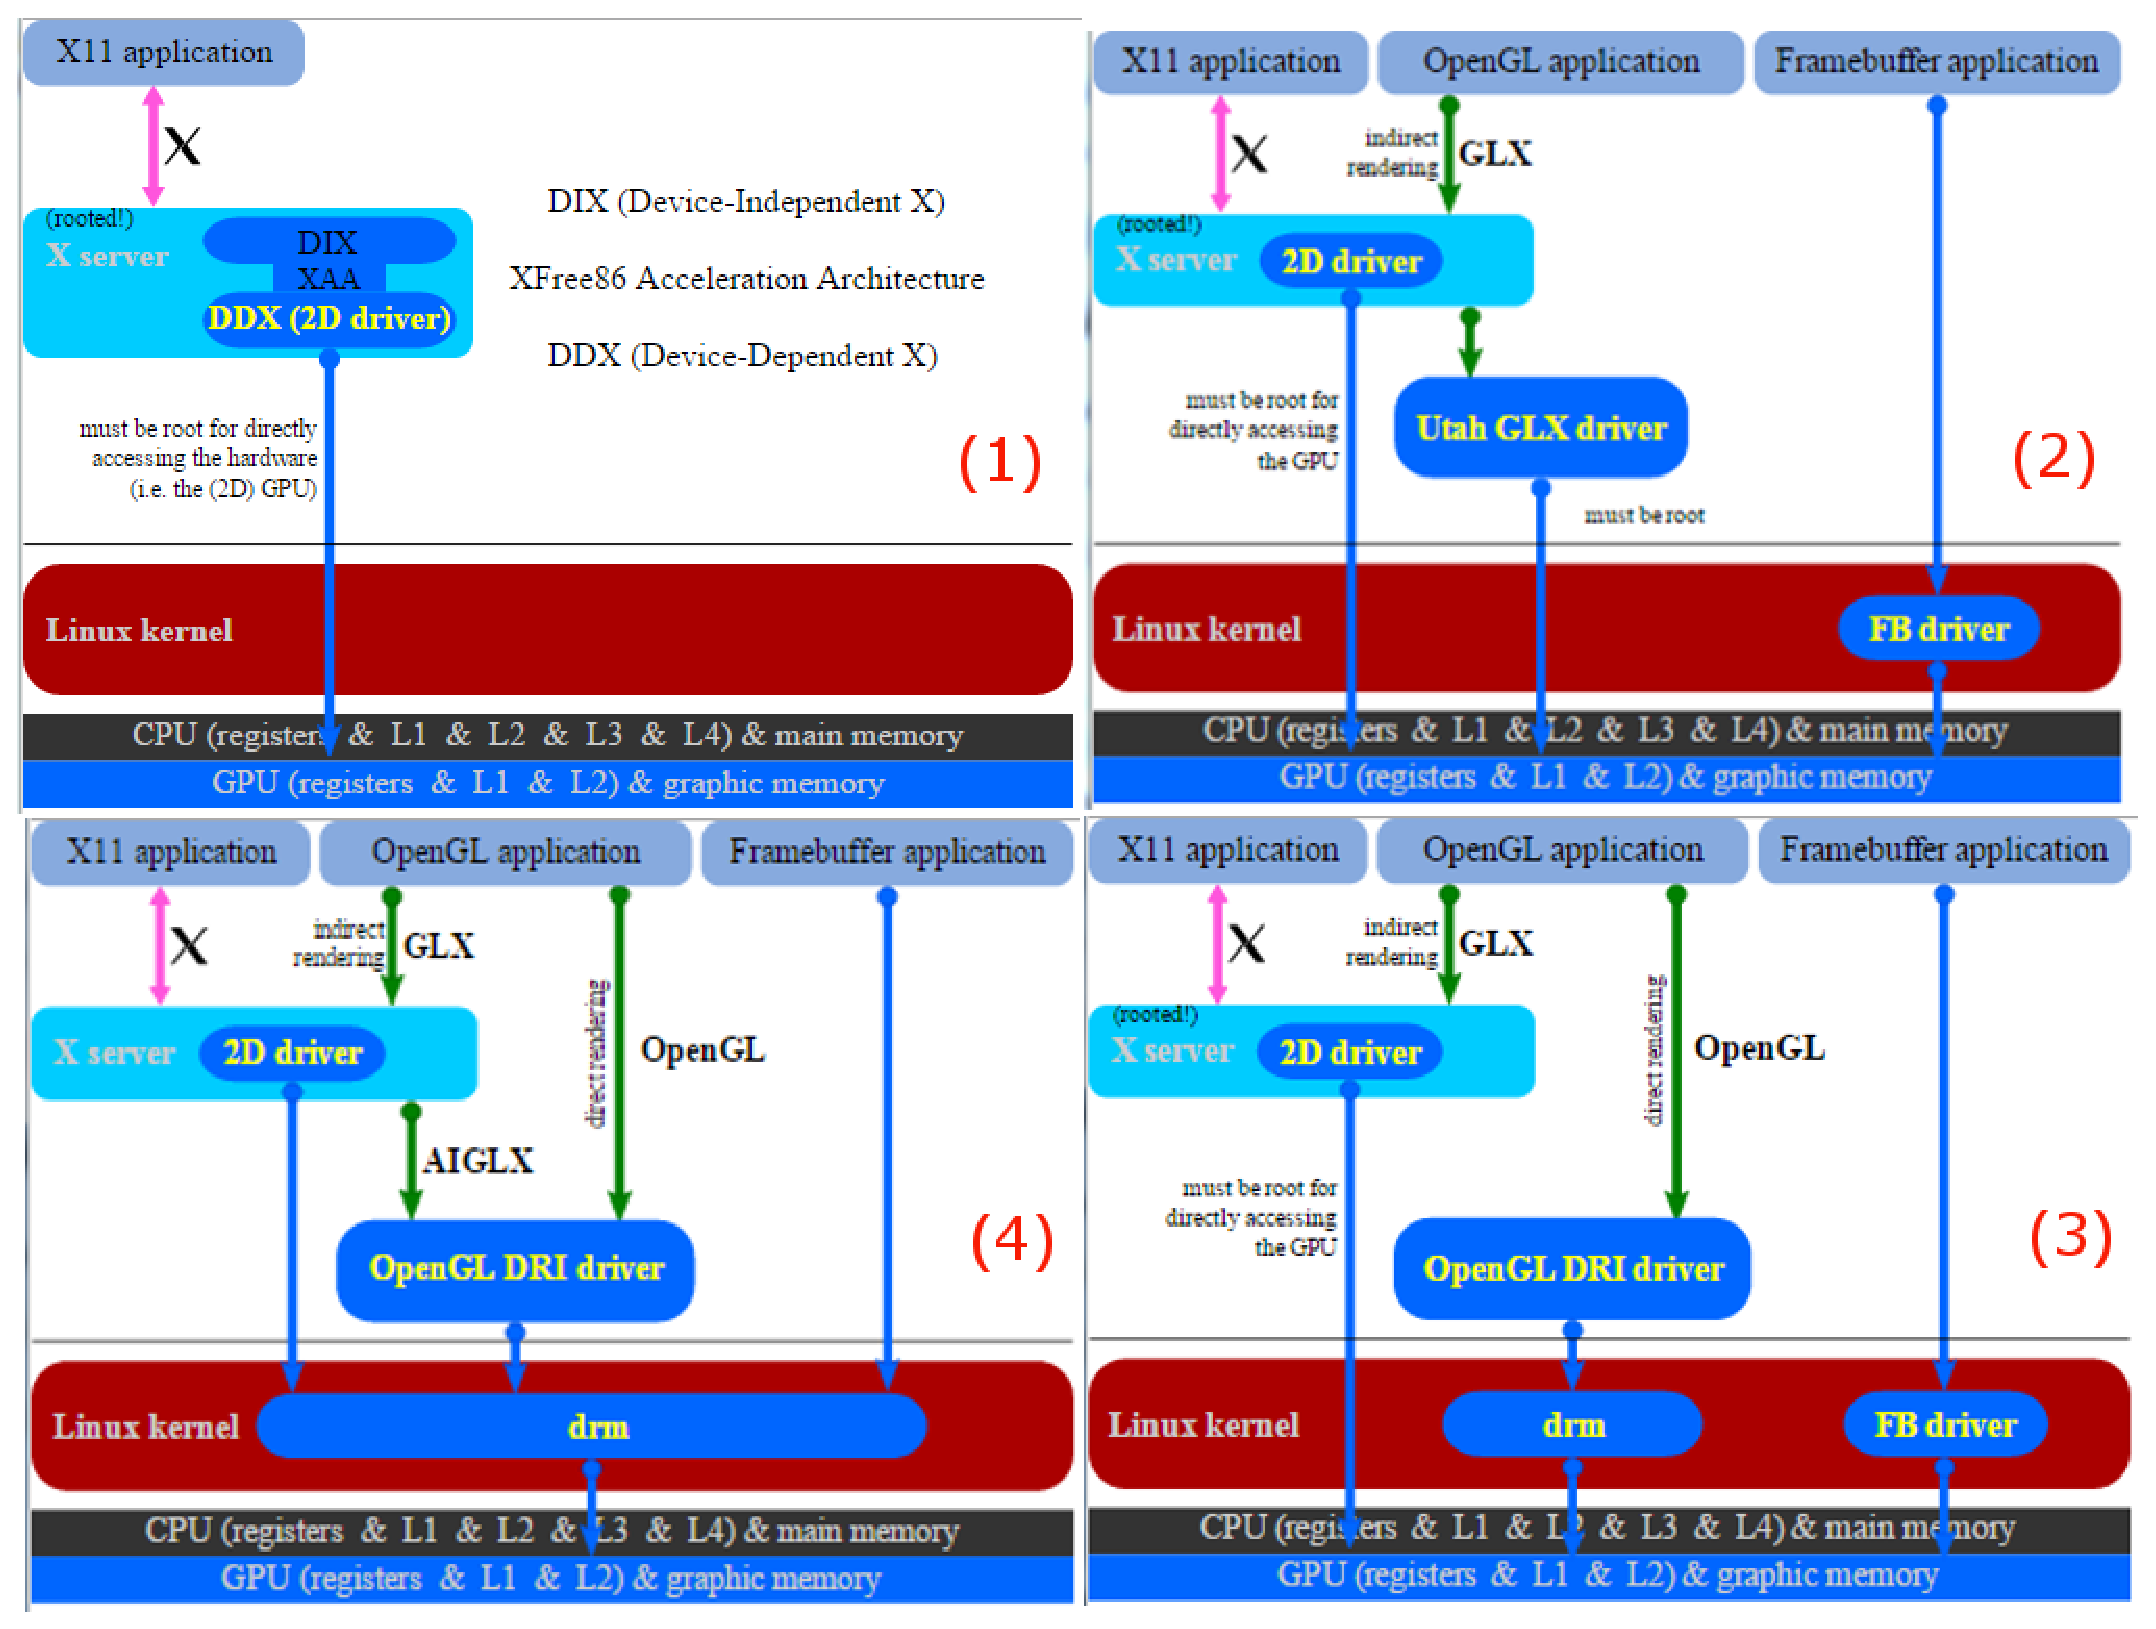
\includegraphics[height=10cm,
    angle=0]{./images/XServer_rendering.eps}}
\caption{Different rendering techniques at different versions of X Server: (1)
2D driver inside X Server (DDX = XFree86 2D), (2) Utah GLX for 3D indirect
direct rendering of OpenGL applications, (3) Early DRI architecture with OpenGL DRI driver, (4) DRM
controls all direct access to graphics hardware}
\label{fig:XServer_rendering}
\end{figure}



\subsection{What is 3D graphics: perspective and surface
lighting/shading, texture mapping, blending}

3D refers to objects that have width, height and depth. However, in
computer graphics, they are displayed on 2D monitor. So, it requires
algorithms for projecting ... in such a way that provide an illusion of
depth. This is known as {\bf perspective} (\verb!glPerspective()!
which tells the angle between the lines that tells the illusion of
depth).

However, perspective is not enough to provide you a true 3D
feeling. Another information that you need is {\it surface shading}
due to lighting, and the relative size of different objects.
This is known as {\bf foreshortening}. 

\begin{framed}
  In summary, all that we need to create 3D feeling are perspective,
  foreshortening, color change, texture, shading and variation of
  color intensities. 
\end{framed}

The process of transforming a mathematical and image data into 3D
image on the display is called {\bf rendering}. One of the process in
rendering is {\bf transformation and projection}. 
\begin{itemize}
\item transforming = moving the points (i.e. {\bf vertices}) around so
  that the line connecting them produce the illusion of a 3D world on
  a 2D display. To move the points, we need a {\bf transformation
    matrix}, and to convert the 3D coordinates onto a 2D display, we
  need another matrix - called {\bf projection matrix}. 
\end{itemize}

2D display is indeed a matrix of pixels. So, to make a line, we need
to fill the pixels with appropriate colors. This process is known as
{\bf rasterization}. One technique often used during this process is
{\it hidden surface removal}. Not only lines (i.e. wireframe
rendering), but also solid geometric primitives (triangles, polygons)
are also rasterized, i.e. we need to fill color on a surface, not only
a single line. OpenGL provides APIs for filling colors into geometric
primitives.

\begin{framed}
  Primitives are one- or two-dimensional entities or surfaces like
  points, lines, triangles, polygons that are assembled into a 3D
  space to form 3D objects.

  A vertex is nothing more than a coordinate in 3D, with
  color/normal/... information. Creating a solid 3D geometry is little
  more than a game of ``connect-the-dots''. 
\end{framed}

In addition to filling a solid color, there is a need of {\bf
  shading}, i.e. varying the color across the surface. This will
create the effect of light shining on a red cube. 
\textcolor{red}{Lighting and shading is a major part in 3D computer
  graphics}. 


Not only filling the color on a surface, you may want to fill it using
a given picture. This is known as {\bf texture mapping}. This adds a
whole new level of realism to our rendering. 

Another level of realism is {\bf blending}, which allows you to add
``mirroring'' effect, i.e. transparency. 


\subsection{Real-time vs. Non-real-time 3D}
\label{sec:real-time-vs}

In real-time, your input cause a change in the 3D visualization within
an unnoticeable time. 

In non-real-time 3D, normally the result is very high quality
image. So, rendering a single frame may need lots of computational
processing, and thus time. In 3D movies, ones design the models and
scenes or ones can use a program (Maya, ...) to create the content,
then the results is sent to a ray tracer (scan-line renderer) to
generate the 3D images.  Thousands of frames are generated and then
combined to form a 3D movies, though the content is not interactive.
\subsection{X11 - 3D: GLX, DRI}
\label{sec:X11-3D}

Direct graphics hardware access support for X Server started with 3dfx GlideAPI
in the Mesa implementation for Voodoo GPU (Sect.\ref{sec:mesa-3d}).

There was another effort to develop hardware driver for the alternative X Server
implementation, XFree86 (Sect.\ref{sec:XFree86}), that lead to
the {\bf Direct Rendering Infrastructure} (DRI) - the foundation for 3D graphics
support on Linux. 

To help resolve the problem with two programs trying to control the same video
card at the same time, the {\bf drm} component (Direct Rendering Manager) was
added to the Linux kernel, Fig.\ref{fig:XServer_rendering}(3)(4).

The DRM gets an exclusive access to the video card, and it's responsible for
initializing and maintaining the command queue, the VRAM and any other hardware
resource. The programs that want to use the GPU send their requests to DRM,
which acts as an arbitrator and takes care to avoid possible conflicts.
\url{http://en.wikipedia.org/wiki/Direct_Rendering_Manager}

\subsection{ -- GLX}

GLX provides extensions to X11 to provide this functionality, ie taking client
OpenGL calls and passing them on to the OpenGL libraries, which can also involve
encapsulating these commands to be passed across a network connection.


\subsection{OpenGL (2D/3D) specification}
\label{sec:OpenGL}

To avoid to much effort, and to much duplication for doing the same work, a
de-factor standard need to be used among hardware manufacturers. {\bf IRIS GL
API} for 2D graphics from Silicon Graphics (SGI) became the dominant in early
1990s (early to use, support immediate mode rendering).
OpenGL specification was first developed in 1991 and released in 1992 - for
advanced scientific simulation (Chap.\ref{chap:opengl}).

With the emerging of 3D graphics hardware, SGI released new opening
standard OpenGL (version 1.0) in 1992 with the creation of OpenGL ARB
(Architectural Review Board), supporting 3D interface.

Initially (since 1991), OpenGL was designed to work on high-end hardware for
engineering and CAD uses, e.g. virtual reality (VR), flight simulation. OpenGL
is a C library, designed to be cross-platform, so it provide abstract APIs
specification for 2D/3D graphics. OpenGL is currently managed by a non-profit
consortium Khronos Group.
\begin{Verbatim}
  OpenGL = {\bf Open G}raphics {\bf L}ibrary: a standard
  cross-platform API specification for writing application that
  produce 2D/3D graphics.
\end{Verbatim}

As 3D gaming grew, OpenGL developed to include better support for programming
techniques for interactive multimedia applications like games, giving developers
choice between using OpenGL or Direct3D (Sect.\ref{sec:Direct3D}).

For OpenGL implementation, read Sect.\ref{sec:OpenGL_implementation}.
% \textcolor{red}{The 3D graphics library are hardware-accelerated, i.e. using GPU
% for rendering}.


\subsection{-- OpenGL ES}
\label{sec:OpenGL-ES}

OpenGL ES is an embedded subset of the industry-standard OpenGL 
graphics platform. It 
\begin{itemize}
  \item   replaced floating  point  arithmetic with fixed point 
  
  \item lack of a GLUT (Sect.\ref{sec:glut-2})
\end{itemize}
while still providing a feature set matching that 
of stationary PCs.

It also expose  the  video  hardware  of  a device,  with  much  of  the 
functionality  available  only  if  the appropriate  video  hardware  is 
available.

\subsection{Direct3D}
\label{sec:Direct3D}

In 1995, Microsoft released Direct3D (a part of DirectX), the current main
competitor of OpenGL. We know many programming languages (C,C++, Fortran), but
the code runs on CPU. Microsoft released HLSL (High Level Shading Language), a
programming {\it shading} language to use Direct 3D API to build a {\bf shader}
with shader construction using C-like syntax, types, expressions, statements,
and functions. A shader is a binary file to run in GPU (Sect.\ref{sec:shaders}).


In 2014,  Microsoft announces DirectX 12.
The main difference from DX11 is the significantly reduced driver overhead, and
more direct access to hardware.

\subsection{-- Direct3D Mobile}
\label{sec:Direct3D-Mobile}

Direct3D  Mobile   has  a  similar  API  to  DirectX  8.0
(Sect.\ref{sec:DirectX}), but lacks most of the  more advanced  features  used 
in  many  game  titles  for  stationary PCs.
Also, several API changes such as replacing floating point 
arithmetic with fixed point to target mobile devices.




\subsection{GlideAPI: 3dfx}
\label{sec:3dfx}
\label{sec:GlideAPI}

3dfx make the Voodoo line of 3D cards, and Glide is 3Dfx's proprietary graphics
language. The Glide API was their own custom API (like Direct3D or OpenGL) that
takes advantage of the Voodoo hardware.

The source is then made available
\url{https://sourceforge.net/projects/glide/files/?source=navbar}. Nowadays, the
best parts of Glide is integrated into future versions of OpenGL:
3dfx have joined the OpenGL ARB.

Glide is based on the basic geometry and "world view" of OpenGL. GlideAPIs only
contains selected APIs primarily useful for real-time rendering of 3D games.





\subsection{glitz}
\label{sec:glitz}

{\bf Glitz} is a 3D graphics library (software library), and
provide hardware acceleration for 2D graphics using OpenGL
(Sect.\ref{sec:OpenGL}).

The development of glitz has been ceased. Cairo library (Sect.\ref{sec:cairo})
uses glitz as the backend.

\subsection{cairo}
\label{sec:cairo}

{\bf Cairo} (stylized as cairo) is a library used to provide a vector
graphics-based, device-independent API. It uses a number of different backend to provide 
hardware acceleration when available.
\begin{itemize}
  \item {\bf glitz} library (Sect.\ref{sec:glitz})
  \item {\bf Xlib}
  \item {\bf XCB}
  \item Win32GDI - Sect.\ref{sec:Win32GDI}
  \item binary files: PNG, PDF, PostScript, SVG
  \item DirectFB - Sect.\ref{sec:DirectFB}
  \item OS/X Quartz Compositor - Sect.\ref{sec:Quartz_compositor}
  \item Microsoft's Direct2D - Sect.\ref{sec:Direct2D}
  \item Skia
  \item Qt
  \item OpenVG

\end{itemize}

The library itself is being used as the backend in many widget toolkits
(Sect.\ref{sec:widget-toolkits-list}).
\begin{itemize}
  \item FLTK - Sect.\ref{sec:FLTK}
  \item GNUsteps
  \item GTK+ 2.8+ - Sect.\ref{sec:GTK+-2.8}
\end{itemize}

\url{http://en.wikipedia.org/wiki/Cairo_(graphics)}

For 3D rendering, use {\bf Cogl} (Sect.\ref{sec:Cogl}).

Cairo can use Cogl to draw; Cogl will program the GPU pipeline, but Cairo will
generate the geometry to be submitted, so you can have high quality 2D results.
Cairo already can use GL directly, but Cogl has a better state tracking already.

\subsection{Cogl library}
\label{sec:Cogl}


Cogl is a GPU programming library that internally can use GL or GLES to access
the graphics pipeline (though in theory it could as easily use DirectX on
supported platforms).

Cogl is a 3D graphic library based on OpenGL(or a fork? I don't know), and
Clutter is a 3D GUI toolkit based on Cogl (Sect.\ref{sec:Clutter}).

\subsection{Clutter library}
\label{sec:Clutter}

Clutter uses Cogl for 3D rendering, but it can also use Cairo for 2D elements
(Sect.\ref{sec:cairo}).

IMPORTANT:
Clutter will not replace GTK+ (Sect.\ref{sec:GTK+}): GTK+ is a very complex
library that provides system integration, complex widgets, and other utility API
that Clutter has no interest in providing.


Clutter can use GDK, the GTK+ windowing system API, to talk to the windowing
system surfaces and get input events.


In the future, it's entirely possible that GTK+ will use Clutter internally as
the base for its widgets - though that's still a work in progress.
\begin{verbatim}
  GPU <- [ [ Cogl + Cairo ] <- [ GDK + Clutter ] <- GTK+ ] <- application
\end{verbatim}





\subsection{Epoxy library (libepoxy)}
\label{sec:libepoxy}
\label{sec:Epoxy-lib}

Epoxy is a library for handling OpenGL function pointer management for you.

\url{https://github.com/anholt/libepoxy}

Epoxy is a good, compact library called libepoxy that handles all of the needed
OpenGL function dispatching on all of the target platforms - and is even in use by
other mature projects like KDE.

It supports
\begin{verbatim}
GL 4.6 core and compatibility context support.
GLES 1/2/3 context support.


\end{verbatim}


\section{Future 2D/3D graphics library}

While OpenGL still carries 20 years of baggage along with it, it's not
unreasonable to beleive that OpenGL may be fighting for its survival over the
next few years.

The goal will be Approaching Zero Driver Overhead (AZDO). The problem is
\begin{itemize}	
  \item the app can handle more
  \item the GPU can handle more
\end{itemize}
but the driver reaches the limits, i.e. overhead in calling driver API.
\url{http://gdcvault.com/play/1020791/}

Mantle only currently works with certain AMD hardware on Windows. Metal only
works on iOS. DirectX 12 will only work on Windows. OpenGL is the only truly
cross-platform option


\subsection{DirectX 12}

\subsection{OpenGL 4.5}

The current APIs of OpenGL on your machines are 
\begin{itemize}
  \item at least, the implementation from multi-vendors (EXT identifiers) and
  mostly cores from OpenGL 4.2+
\end{itemize}

Among other things, 4.5 finally, brings Direct State Access (DSA) into
core. 
\begin{verbatim}
## Before DSA
glBind(something)
glSetA(..)
glSetB(..)
glSetC(..)

## With DSA
glSetA(something, ..)
glSetB(something, ..)
glSetC(something, ..)
\end{verbatim}

\subsection{Mantle (for AMD GPUs)}
\label{sec:Mantle}

In September of 2013, AMD announced a new, low-level graphics API called Mantle,
designed to be an alternative to OpenGL and Direct3D.

The idea with Mantle was to allow direct access to AMD hardware with an absolute
minimum of driver overhead, something that OpenGL and DirectX didn't really
offer at the time. AMD boasted that Mantle offered large performance gains
compared to "other APIs."

\subsection{Metal (for iOS)}
\label{sec:Metal}


In July of 2014, Apple follows suit and releases its own low-level graphics API
called Metal. Prior to Metal, OpenGL ES was the only option for iOS devices.

Metal is implicitly meant to work with shared memory architectures which only
maps to Intel on Desktops currently.
Someone said: ``{\it For Apple 70\% computers sold are Laptops which means Intel
GPU. Apple is not going to drop Metal as it is doing custom GPUs.
Will CAD manufacturers support Vulkan then Apple may be forced
otherwise don't bet a dollar. Apple may support SPIR-V if it came with LLVM compiler but not much else.
It may even back away from OpenCL especially in mobile environment.}
 
\subsection{glNext (codename: Volkan)}
\label{sec:glNext}

So far, on Linux, OpenGL is the only API available for hardware accellerated 3D.
However, after 20 years, the architecture of GPUs nowadays are very different
from the early days, e.g. unified memory and tiled rendering, with many more
different platforms (smartphone, hand-held game player, smart devices in cars,
\ldots). glNext is a ground-up re-design of API for high-efficiency access to
graphics and compute on modern GPU and platforms (Chap.\ref{chap:Vulkan}).




\section{CPU-based vs. GPU-based APIs}

\subsection{GPU-based graphics APIs (Graphic Hardware APIs)}

There are many libraries that implement APIs that utilize Graphic Hardware
\begin{enumerate}
  \item DirectX
  
  \item  TwGfx: on the TapWave Zodiac device
\end{enumerate} 

\subsection{CPU-based graphics APIs (frame-buffer APIs)}
\label{sec:Frame-Buffer-API}

 
Frame-Buffer  APIs,  which  provide  software-based rendering  operations  that 
draw  graphics  directly  into  the  frame buffer  of  the  device,  using  only
 the  CPU  as  a  graphics  engine.
\begin{itemize}
  \item  PocketFrog  on  Windows  Mobile,  and  
  
  \item Razor  on the Palm platform
\end{itemize}


\section{Understanding screen and pixel}

Important   hardware   variations   include   frame   buffer  orientations,
cache  memory  sizes,  memory  access  latencies  and timer  granularities

\subsection{raster scan display}
\label{sec:raster-screen}


A raster display is a collection of dots called pixels,
Fig.\ref{fig:raster-display}. The pixels are constantly updated, with colors and
brightness via a given updating strategy.
A a raster display is a matrix of dots, and the color at each pixel updated by a
tracing beam scanning crossing the display (Sect.\ref{sec:refresh-procedure}).

The screen is continuously updated, by painting the whole screen, the tracing
beam scans at a rate high enough to prevent flickering, e.g. a proper refresh
procedure (Sect.\ref{sec:refresh-procedure}), at a rate of 60 to 80 frames per
second. The information of picture is retrieved from a frame buffer
(Sect.\ref{sec:frame-buffer}).

\begin{figure}[hbt]
  \centerline{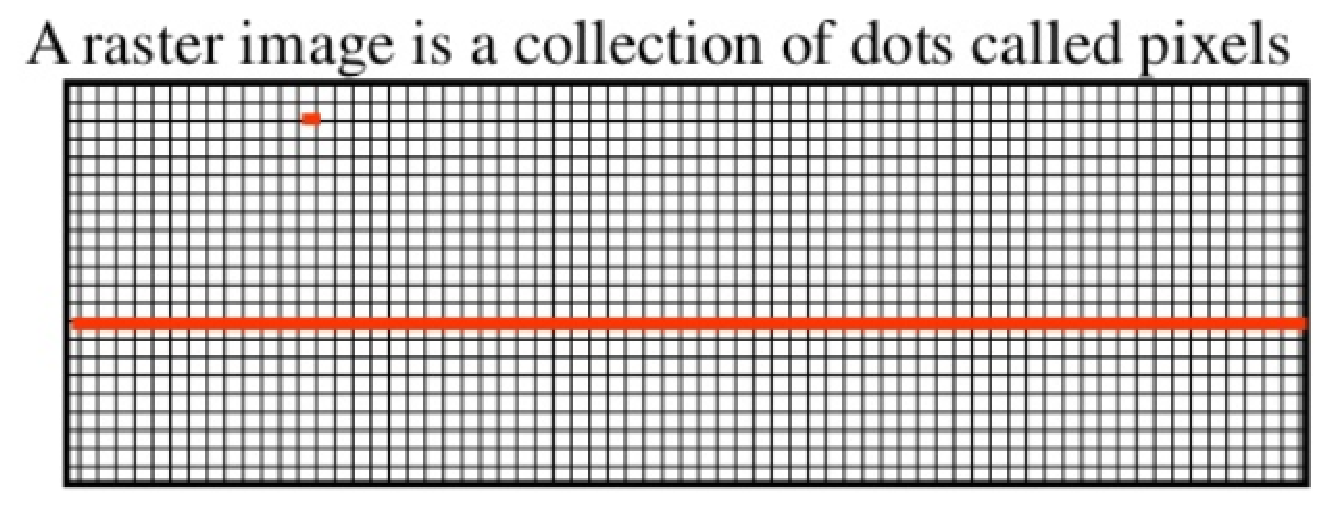
\includegraphics[height=5cm,
    angle=0]{./images/raster-display.eps}}
\caption{A raster display is a collection of dots called pixels}
\label{fig:raster-display}
\end{figure}

To draw a picture of a screen, we need the display controller
(Sect.\ref{sec:display-controller}) which draw the image stored in the memory
region (Sect.\ref{sec:frame-buffer}), following a certain refres procedure
(Sect.\ref{sec:refresh-procedure}).
  
\subsection{video controller (display controller)}
\label{sec:display-controller}

The display controller is a special processor, not the CPU, that control the
operation of the display device (Sect.\ref{sec:raster-screen}). 
This display controller read and process data from the frame buffer
(Sect.\ref{sec:frame-buffer}) and then can send image data to the terminal
display (e.g. printer, monitor, ..). If the terminal is the monitor
(Sect.\ref{sec:raster-screen}), the tracing beam following a given
strategy (Sect.\ref{sec:refresh-procedure}) to generate the exact content on
the screen.


To draw images to the terminal display, developers have to manually  convert RGB
color  values  into  the  current native screen format. Example: To  convert  an
RGB  value  to native  screen  format,  the  processor has  to  perform  up  to
ten operations  for  each  pixel  (four  AND,  three SHIFT  and  three  OR for
the  Palm  device). Since  this  is  a  costly  operation,  images  should  be
pre-rendered  to match  the  native  format  of  the  frame buffer   before  
being   used   in any   graphics   operations.
\begin{itemize}
  \item refreshing the screen
  
  \item transformation (e.g. enlarge a certain area, move a window)
  
\end{itemize}

% and  write  them  as
% bytes  to  the  frame  buffer  of the device (Sect.\ref{sec:frame-buffer}). This
% requires
% \begin{enumerate}
% 
%   \item cache  optimizations when  reading  and  writing  pixel  data  to  the  display  frame  buffer.
%   
%   \item   
% \end{enumerate}
% 


\subsection{refresh procedure}
\label{sec:refresh-procedure}

An image is divided into a sequence of (usually horizontal) strips known as {\bf
scan lines}, which can be further divided into discrete pixels for processing.
Each time the display controller (Sect.\ref{sec:display-controller}) needs to
update the screen, it controls the tracing beam following one of the below procedure
\begin{enumerate}
  \item  {\bf line by line}: the tracing beam scan from left to right, and then
  repeat to the next line. Lines start from first line, and once it reaches to the
  right most pixel on the last line, the tracing beam return to the left most of
  the first line.
  
This may cause flicker on raster display with slow refresh rate.
\begin{itemize}
  \item Horizontal retrace: (the electron beam follows horizontal tracing)
  refers to the return to the left (on next line) of the electron beam
  
  \item Vertical retrace: refers to the return to the top left corner of the
  electron beam
\end{itemize}

  
  \item {\bf interlacing}: there are two phases: even field and odd field.
   
   \item {\bf random-scan }: the electron beam directed to only the parts of
   the screen where a picture is to be drawn.
   
   It draws a picture one line at a time (vector display or stroke-writing or
   calligraphic display). So to draw a picture, the system goes through a set of
   commands in the {\bf display file} (display list), drawing each component
   line in turn.
 \begin{verbatim}
 Move 100,100
 Draw 200,140
 Text "hello!"
 Move 40,12
 ...
 
 Draw 100,1
 Jump start
 \end{verbatim}
   
   All components of a picture is drawn, i.e. refreshed, at a rate 30 to 60
   times per second.
   
   CONS: random-scan display only works well for line-drawing application; but
   not for realistic shaded scenes.
   
   
\end{enumerate}



\subsection{frame buffer: where picture is stored? (double buffer, triple
buffer, vsync)}
\label{sec:frame-buffer}
\label{sec:double-buffer-frame-buffer}
\label{sec:triple-buffer-frame-buffer}

When a computer needs to display something on a monitor, it draws a picture of
what the screen is supposed to look like and sends this picture (which we will
call a {\bf buffer}) out to the monitor.

\begin{itemize}
  \item  In the old days there was only one buffer and it was continually being
  both drawn to and sent to the monitor. 

ISSUE: when objects on the display were updated, they would often flicker.
  
  \item In order to combat the issues with reading from while drawing to the
  same buffer, {\it double buffering}, at a minimum, is employed.

The idea behind double buffering is that the computer only draws to one buffer
(called the "back" buffer) and sends the other buffer (called the "front"
buffer) to the screen. 

 After the computer finishes drawing the back buffer, the program doing the
drawing does something called a buffer "swap." This swap doesn't move anything:
swap only changes the names of the two buffers: the front buffer referencing
to the location of the back buffer and the back buffer referencing to the
memory location of the previous front buffer.

ISSUE: in this form of double buffering, a swap can happen anytime. That means
that while the computer is sending data to the monitor, the swap can occur. When
this happens, the rest of the screen is drawn according to what the new front
buffer contains. If the new front buffer is different enough from the old front
buffer, a visual artifact known as "tearing" can be seen. 
This type of problem can be seen often in high framerate FPS games when whipping
around a corner as fast as possible.  Because of the quick motion, every frame
is very different, when a swap happens during drawing the discrepancy is large
and can be distracting. 

  \item {\bf vsync}: Synchronizing buffer swaps with the Vertical refresh is
  called vsync.
  
Here, it waits to swap buffers until the monitor is ready for another image.
While enabling vsync does fix tearing, it also sets the internal framerate of
the game to, at most, the refresh rate of the monitor (typically 60Hz for most
LCD panels).

NOTE: With 60Hz, every frame takes just a little longer than 16.67 ms.

ISSUE: Input lag also becomes more of an issue with vsync enabled. This is
because the artificial delay introduced increases the difference between when something
 actually happened (when the frame was drawn) and when it gets displayed on
 screen.
 
NOTE: Input lag always exists (it is impossible to instantaneously draw what is
currently happening to the screen), but the trick is to minimize it.
  
   \item {\bf triple buffering}: it combines the best of both worlds with no
   sacrifice in quality or actual performance.
   
   
 There are 3 buffers: two back buffers, and one front buffer. This additional
 back buffer gives the computer enough space to keep a buffer locked while it is
 being sent to the monitor, i.e. if the new image is needed, it updates to the
 other back buffer, i.e. not affecting the buffer being sent to front buffer.
 Also, each time, the  front buffer is swapped for the back buffer containing
 the most recently completed fully rendered frame.
 
   \item {\bf flip-chain}:  multiple back buffers in a flip chain. A flip chain
   is simply two or more back buffers (sometimes called intermediary buffers)
   plus the primary surface (this is sometimes called triple-buffering,
   quadruple-buffering, etc.).   
   
 You have more than two back buffers. This is particularly useful when the
 amount of time spent drawing is greater than the monitor's refresh rate. 
 
In a flip chain, the next available back buffer becomes the primary surface,
 etc., all the way down to the rearmost back buffer that is used for drawing.
\end{itemize}
\url{https://docs.oracle.com/javase/tutorial/extra/fullscreen/doublebuf.html}

% Regardless of the type of image, i.e. raster or vector format, to be drawn
% (displayed) on a terminal, there must be a region where such information is
% stored. The picture definition (to be displayed on the monitor) is stored in a
% memory region called {\bf frame buffer} or {\bf refresh buffer}. 

Each terminal device has its own front framebuffer, that the display controller
(Sect.\ref{sec:display-controller}) understand and can read it.

Suppose the terminal is monitor, the information for each pixel, is called the
{\bf depth}, which can be
\begin{itemize}
  \item simply 1 bit per pixel (for black-and-white monitor). 

This frame buffer is called {\bf Bit map}.

  \item 16bits per pixel (i.e. 2 bytes/pixel)
  

  \item 24bits per pixel (typically holds RGB components, each with 8bits).
  
\end{itemize}
The order is also important: 
\begin{itemize}
  \item  Little Endian format: Palm O/S 5
  
  \item Big Endian: 
\end{itemize}

Basically, each location on the frame buffer holds the intensity values for the
associated pixel on the raster screen (Sect.\ref{sec:raster-screen}).
The pixel data in this frame buffer will be read in by the display controller
(Sect.\ref{sec:display-controller}), through a series of operations, before
painting a proper intensities on the monitor at the position associated with the
read-in pixel.

\subsection{frame buffer orientation}
\label{sec:frame-buffer-orientation}

For  design  reasons,  displays  are  internally  aligned  differently  on
various mobile devices, Fig.\ref{fig:framebuffer-orientation}. Form factor is
important, and the display and  its  connector  are  often  rotated  90  or  180
 degrees  to  decrease the physical size of the device. Currently there are
mobile devices available  with  all  of  the  four  possible  frame  buffer 
orientations.
\begin{itemize}
  \item \verb!xPitch! : numberof bytes need to add to move to the next pixel
  (on the same line)
  
  \item \verb!yPitch!: the number of bytes needed to add to move to the pixel on
  the next row.
\end{itemize}

\begin{figure}[hbt]
  \centerline{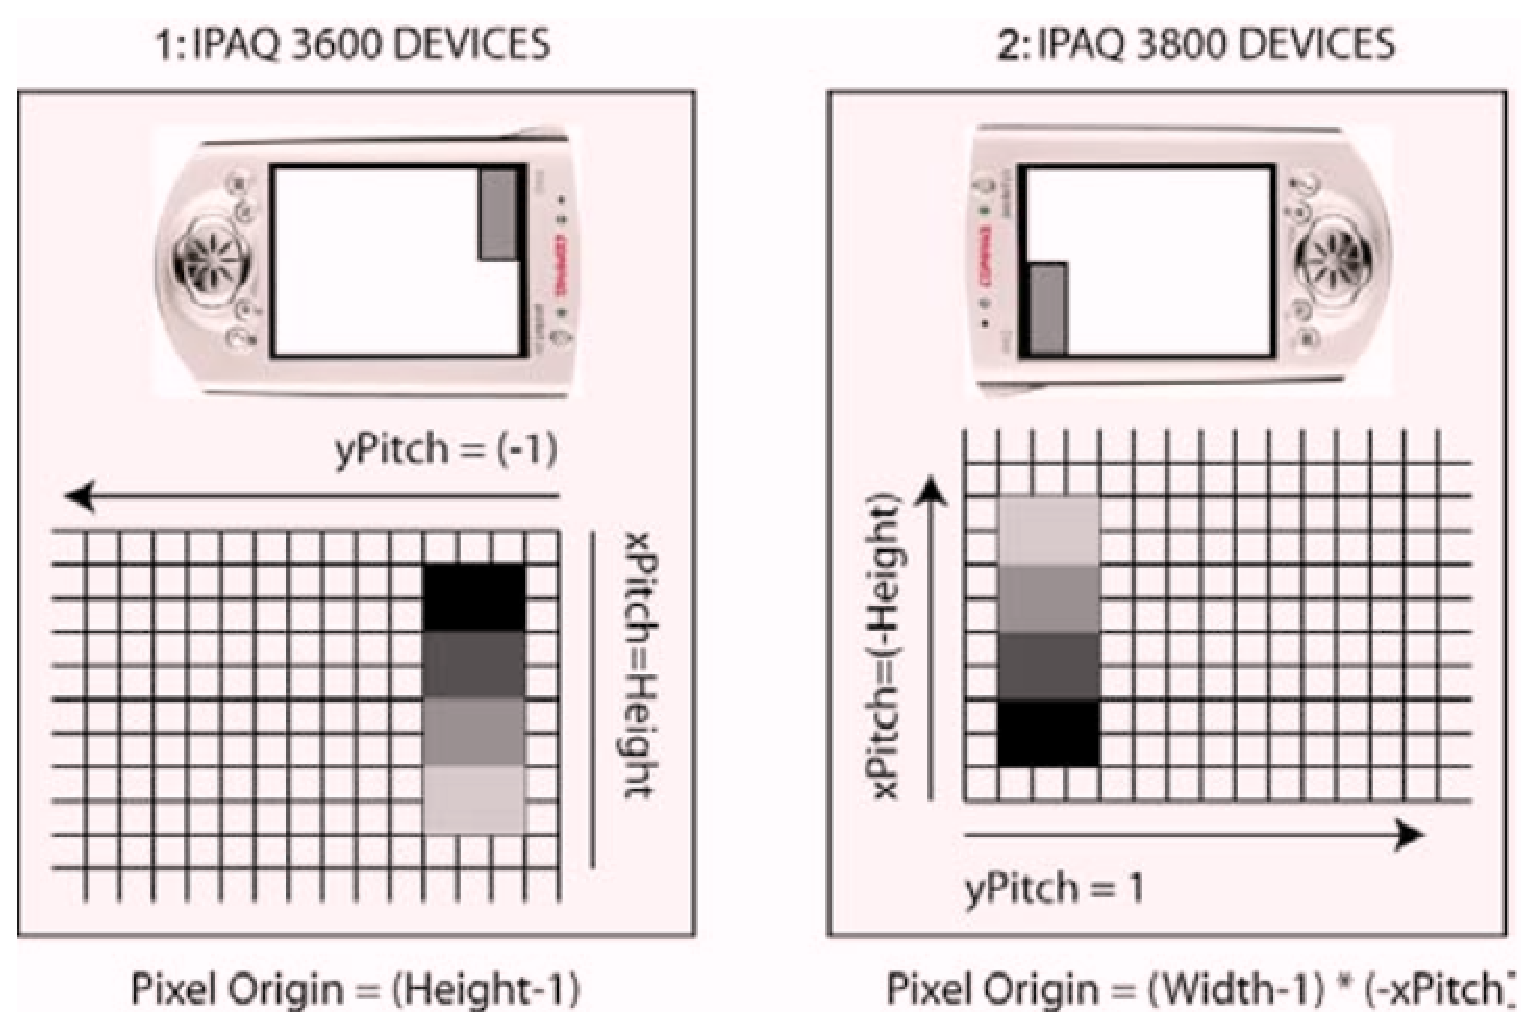
\includegraphics[height=5cm,
    angle=0]{./images/framebuffer-orientation.eps}}
\caption{Frame buffer orientation}
\label{fig:framebuffer-orientation}
\end{figure}

\subsection{Cache line and Data caches}

{\bf Cache line}: Reading  a  single  byte  from  any  location  in  memory 
will automatically  cause  a  computer  to  read  an  additional  number  of
consecutive  bytes  (a cache  line )  and  place  that  in  the  data  cache.
\begin{enumerate}
  \item ARM  CPU,  the  size  of  the  
cache line is 32 bytes

Reading  the  first  pixel  will  cause  the cache to automatically contain the
second, third, and up to the 32 nd pixel  of  that  same  row.

 \item 
\end{enumerate}
The {\bf data caches} stores a number of cache lines, i.e.
ARM  CPU  stores  256  cache  lines,  which  equals  
8kb  of  data  cache.

The  advantage  of  using  a  data  cache  is  that  data retrieved  from  the 
cache  is  accessed  significantly  faster  from  it than data from the main
system memory.




\section{History of widget toolkits}
\label{sec:history-widget-toolkits}

In early days of 1980s, it's not easy to create a GUI software that run on
different graphics hardware. The interface is not unique, i.e. it may looks
diffent when running on different hardware. Also, the manufacturers of the
graphics hardware need to develop the driver for each hardware.

X (Sect.\ref{sec:X11}) doesn't tell how the window or menu or button look like.
These are done by higher-level application software like 
\begin{enumerate}
\item window manager (e.g. twm, nautilus, ...)
\item GUI widget toolkit
\item desktop environment (e.g. KDE, GNOME, Windows...)
\end{enumerate}


\subsection{What is a widget?}
\label{sec:widget}

A widget, which is a combination of an X window and its associated input and
display semantics and which is dynamically allocated and contains state
information.

Widgets can be used
\begin{itemize}
  \item to display information (e.g. text or graphics) : textbox, \ldots
  
  \item as container for other widgets: e.g. menu box
  
  \item for output only and no interact with keyboard or cursor input :
  
  \item to response to input by invoking function that an application has attach
  to it.
\end{itemize}

Every widget belong to exactly one widget class. Logically, a widget class is
the procedures and data associated with all widgets belonging to that class.
Physically, a widget class is a pointer to a structure. The contents of this
structure are ``constant'' for all widgets of the widget class but will vary from
class to class. ``Constant'' means the class structure is initialized at compile
time and never changed, except for one-time class intialization of resource
lists when the first widget of the class is created.


\subsection{Xt}
\label{sec:Xt}

{\bf Xt} libray (Intrinsics) is the library developed on top of Xlib
(Sect.\ref{sec:Xlib}) with APIs to support the creating and using GUI components
starting from basic widgets (e.g. buttons, scrollbars) to complex (e.g. control
panels, property sheets), but still it has {\it no impose on the look and feel
of the widgets yet}.

These GUI components are collectively called {\bf widgets} -
Sect.\ref{sec:widget}. The libraries to provide the look-and-feel of these
widgets is described in Sect.\ref{sec:look_and_feel_specifications}.

Xt uses object-oriented programming techniques. This
allows extension to the list of available widgets by subclassing the existing or
writing a new wone based on the given conventions.
\begin{itemize}
  \item The root class is named {\bf Core} in the first version of Xt.
  
  \item Since Xt version 4, three non-widget superclasses are added above Core
  class, and the new root class is called {\bf Object}.
\end{itemize}
\url{http://www.x.org/docs/Xt/intrinsics.pdf}

Header files to use
\begin{verbatim}
// If using Intrinsic mechanism only
<X11/Intrinsic.h>
<X11/StringDefs.h>

<X11/Xatoms.h>
<X11/Shell.h>

// If want to implement widgets
<X11/IntrinsicP.h>
\end{verbatim}

\begin{mdframed}

On POSIX-based O/S, the Xt library is called \verb!libXt.a! and to link the
library we use \verb!-lXt!.
\end{mdframed}

\subsubsection{Core class}
\label{sec:Core_class}

The Core widget class contains the definitions of fields common to all widgets.


\subsection{Xaw (widget toolkit)}
\label{sec:Xaw}

Xaw (X Athena Widgets) is the GUI widget toolkit that built on top of Xt
library (Sect.\ref{sec:Xt}) as it imposes the look-and-feel of the different
widgets.

Depending on the widget to use, different header
files may also need to be included
\begin{verbatim}
<X11/Xaw/Label.h>

<X11/Xaw/Scrollbar.h>
\end{verbatim}

Xaw is maintained by X.org Foundation and is available as part of the X Window
System installation. 

However, Xaw has been largely superseded by more sophisticated toolkits like
Motif (Chap.\ref{chap:Motif}), GTK+ (Chap.\ref{chap:GTK+}), and Qt (Chap.\ref{chap:Qt}).  

\subsection{X toolkit (Xaw + Xt)}
\label{sec:X_toolkit}
 
Xt (Sect.\ref{sec:Xt}) and Xaw (Sect.\ref{sec:Xaw}) are collectively known as
the {\bf X Toolkit}.


\subsection{Motif}
\label{sec:Motif}

{\bf motif} is an industry standard toolkit/library for building GUI application
in X windows system since 1980s. Different implementations of the Motif API include Open
Motif, LessTif (Chap.\ref{chap:Motif}).  

\subsection{GLUI}
\label{sec:glui}

GLUI is a library with C++ interface, based on GLUT (Sect.\ref{sec:glut-2}), and
provides some user-control widgets (e.g. buttons, menu...). However, it doesn't
support advanced widgets like in Qt, wxWidgets or FLTK. 

% \subsubsection{FreeGLUT}
% \label{sec:freeglut-1}

% An alternate to GLUT, with some enhancements and less bugs. Read
% Sect.~\ref{chap:glut}


\section{Components in a widget toolkit}
\label{sec:UI-components-widget-tookit}

A UI element is aka a {\bf widget} or a {\bf control}.
A widget toolkit contains the implementation for a number of different classes.
Each class represent a UI element, such as textbox, menu, button, menuitem,
dialogbox, main window\ldots
These classes provides methods to interact with the control, or the data from
the control.

A GUI element is classified into one of the following groups
\begin{enumerate}
  \item GUI Component classes (such as Button, TextField, and Label) -
  Sect.\ref{sec:UI-Component}
  
  \item GUI Container classes (such as Frame, Panel, Dialog and ScrollPane) -
  Sect.\ref{sec:UI-Container}
   
  \item Layout managers (such as FlowLayout, BorderLayout and GridLayout) -
  Sect.\ref{sec:UI-Layout}
   
  \item Custom graphics classes (such as Graphics, Color and Font) - 
  Sect.\ref{sec:UI-custom-graphics-class}
 
\end{enumerate} 


When building a GUI application, we can either do it
\begin{itemize}
  \item programmatically : write the code to create the UI element using the
  above classes, identify its location, it's binding to which container
  
  
  \item drag-and-drop: with the help of GUI builders, you can quickly build a
  GUI application; the builder will generate the code for you, and you only need
  to write code to handle different events, i.e. the event handlers
\end{itemize}
\url{https://en.wikipedia.org/wiki/Widget_(GUI)}

Commercial libraries privdes (1) more UI elements; (2) some nice graphical
representations.

\subsection{Component classes}
\label{sec:UI-Component}

A Comonent class is a minimal class in a Widget Toolkit.

\subsection{-- Button}

There are subclases from Button:
\begin{enumerate}
  \item Radio Button
  
  \item Checked Box
  
  \item Split Button: 
  
  \item Cycle Button
\end{enumerate}

\subsection{-- Combo Box}

A combination of TextBox and an attached Menu or ListBox.
User can either enter the text or select the value from a drop-down list or
ListBox.

\subsection{-- Icon}


\subsection{-- Scrollbar}


\subsection{-- Slider}

control with a handle that can be moved up and down (vertical slider) or right
and left (horizontal slider) on a bar to select a value (or a range if two handles are present).

\subsection{-- List box}

\subsection{-- Spinner}

\subsection{-- Drop-down list}

\subsection{-- Menu}

\begin{enumerate}
  \item Context Menu
  
  \item Pie Menu
\end{enumerate}

\subsection{-- Menu Bar}

\subsection{-- Toolbar}

\begin{enumerate}
  \item Ribbon: an hybrid of menu and toolbar, displaying a large collection of
  commands in a visual layout through a tabbed interface.
\end{enumerate}


\subsection{Containers: group the widgets}
\label{sec:UI-Container}

A Container is used to group one or many Component object
(Sect.\ref{sec:UI-Component}) and/or one or many Container object
(Sect.\ref{sec:UI-Container})

Example:
\begin{enumerate}
  \item Window (aka Frame in some widget toolkits such as wxWidget)
  
  \begin{itemize}
    \item Model window
    \item Dialog Box
    \item Palette Window
    \item Frame (if the main window is Window)
    \item Canvas: a generic drawing element for representing graphical
    information.
  \end{itemize}
  
  
  \item panel
  
  \item tab
  
\end{enumerate}

\subsection{-- Window (Frame): Model window, Dialog box, Palette window,
Canvas, Applet}

\subsection{-- Panel}

\subsection{-- Tab}

\subsection{Custom graphics classes}
\label{sec:UI-custom-graphic-classes}

\subsection{-- Tree View}

\subsection{-- Grid View or DataGrid}

This is a complex widget what is as  a spreadsheet-like tabular view of data
that allows numbers or text to be entered in rows and columns.

\section{Look and Feel specifications}
\label{sec:look_and_feel_specifications}

While X Windows System (Sect.\ref{sec:X11}) is the de-facto standard for Unix
communication between client and server for graphical display, it does not
define the look and feel of the GUI. 

The development of look-and-feel tags along with the development of different
widget toolkits (Sect.\ref{sec:history-widget-toolkits}).

\subsection{OPEN LOOK}
\label{sec:OPEN_LOOK}

To help defining the standard for GUI look-and-feel, in Apr-1988, {\bf OPEN
LOOK} specification was created, a collaboration between Sun and AT\&T. The two
companies then formed OSF (Open Software Foundation) to manage OPEN LOOK.
OSF also created Motif GUI (Chap.\ref{chap:Motif}).

% The first O/S to have a look-and-feel is the Macintosh O/S, yet there is no
% standard in how the GUI components should look like.

OPEN LOOK: overall philosophy was to provide a clean, simple and uncluttered
interface, so that the user's focus would be on the application rather than the
interface. It is a definition of a look and feel rather than a specific
implementation
\begin{itemize}
  \item oval buttons, triangle glyphs: to indicate pull-down and pull-right menus
  
  \item "pushpins" which allowed the user to make dialog boxes and palettes stay visible. 
\end{itemize}


Widget toolkits that were developed using OPEN LOOK specification
\begin{enumerate}
  \item OLIT (OPEN LOOK Intrinsics Toolkit - introduced 1988): built on top of Xt (Sect.\ref{sec:Xt})
  \label{sec:OLIT}
    
  \item XView (introduced 1988): object-oriented API for C language. The source-code was pubclicly released in 1990.
  It is considered as the first open-source professional widget toolkit for X Window System.
  \label{sec:XView}
  
  UIT (User Interface Toolkit) is the C++ API to XView.
  
  XView was reputedly the first system to use right-button context menus, which is ubiquitously used.
  
\end{enumerate}

It is later abondoned in favor of Motif specificatioin (Sect.\ref{sec:Motif_specification})
and more recently GTK+ (Chap.\ref{chap:GTK+})

\subsection{Motif specification}
\label{sec:Motif_specification}

Motif user-interface specification is completely independent of how it is
implemented. So, you do not have to use the X Window System to implement a
Motif-style graphical user interface (GUI).

The first implementation of Motif specification use X Window System and X
Toolkit (Sect.\ref{sec:X_toolkit}) as the platform for the Application
Programmer's Interface (API), Xm library .

\url{http://www.ist.co.uk/motif/books/vol6A/ch-2.fm.html}

% Other widget sets:
% \begin{enumerate}
%   \item Athena widget set (Sect.\ref{sec:Xaw})
%   \item Motif (Chap.\ref{chap:Motif})
% %  \item OPEN LOOK (Sect.\ref{sec:OPEN_LOOK})
% \end{enumerate}


\subsection{Plugable look-and-feel}
\label{sec:look_and_feel_plugable}

Currently, only Swing widget Toolkit feature {\it plugable look-and-feel} - a
mechanism allowing users to change the look-and-feel of the program,
unrelated to the underlying platform.

The configuration file is XML, and can be changed at runtime.

\url{http://en.wikipedia.org/wiki/Pluggable_look_and_feel}


\section{Graphics Frameworks in Windows}

If you want to support Windows XP, using a "legacy" graphics framework is the
logical choice.

Starting at around Windows Vista, Microsoft has been
redesigning many of their API.
\begin{itemize}
  \item MMDevAPI: One True Sound API
  \item WIC: One True Image File API
  \item 
\end{itemize}
These new API's are much better than the old ones, and the "legacy" systems all
work based on the new ones.
Since Windows Vista and later, DirectSound is entirely based on MMDevAPI, and
components that need to read image files do it via WIC.

\subsection{'legacy' system (Windows XP): GDI, GDI+}
\label{sec:GDI}
\label{sec:GDI+}

The status designation of "obsolete" just means that the group responsible is no
longer accepting or fulfilling bug reports (except for critical security issues).

GDI isn't going anywhere, so if you need something rock-solid that is guaranteed
to be supported anywhere and everywhere, that's what I would go with.
If you need a bit more 2D capabilities than GDI offers (e.g., alpha channel
transparency), then you could consider using GDI+.

GDI+ is nearly an order of magnitude slower than GDI, but that's not too big of
an issue on modern machines with more power than you could ever want. This, too,
is going to be supported for a very long time to come.



\subsection{APIs on Windows RT}
\label{sec:GraphicsAPI_Windows-RT}

gdiplus, d3d9, and directdraw are present, but opengl is not.
 
 The only way to develop for Windows RT is through metro (now called the Windows
 8 Store), which restricts the old API's.

\section{Why no hardware-accelerated in 2D widget toolkits for mobile?}

Many features offered by the existing 2D APIs are difficult
or extremely expensive to implement using OpenGL. 

mobile GPUs are tile-based and aren't great in terms of raw pixel processing
power, but the pixel throughput would definitely be miles ahead of a general
purpose CPU.
I'm sure you guys have already considered this angle, but instead of using
OpenGL why couldn't you create a custom 2D graphics library for vendors to
implement at the lower level?

\url{https://groups.google.com/forum/#!topic/android-developers/D0PtrODTwBk}

However,  window composition is already hardware
accelerated and has been so since Android 1.0.

it really depends on what the application does exactly. If you
are always drawing the same translucent bitmap on screen, the GPU will
be better. If you are drawing complex shaded and antialiased paths or
you draw a bitmap that changes often, things can get pretty bad. Some
features of the Canvas API require other kinds of expensive operations
(for instance, implementing saveLayer/saveLayerAlpha requires the use
of FBOs or glCopyTexImage2D and neither solution is ideal.)


 Making a few fast paths for drawing bitmaps (BitBlt) would be huge for 
game developers.  I know that 3 of my games I have made aren't OGL 
simply because I don't want the extra code maintenance/burden.  If a 
game is doing some of the things you mention, well then it's not likely 
concerned with frame-rate.

Use OpenGL ES.


\section{Win32 GDI vs. Xlib}
\label{sec:WIN32_Xlib}

Win32 code using Win32 GDI (Sect.\ref{sec:Win32GDI}), while slightly opaque, is
miles easier to write then xlib code (Sect.\ref{sec:Xlib}). Xlib is miles more
complex then anything else, that is partially due to the fact that it was
developed to be a multi-client server.
\url{http://forums.anandtech.com/showthread.php?t=2054601}

A window created with native Win32 calls is about on the level of difficulty as
using the GTK+ to do the same thing. 

\begin{figure}[hbt]
  \centerline{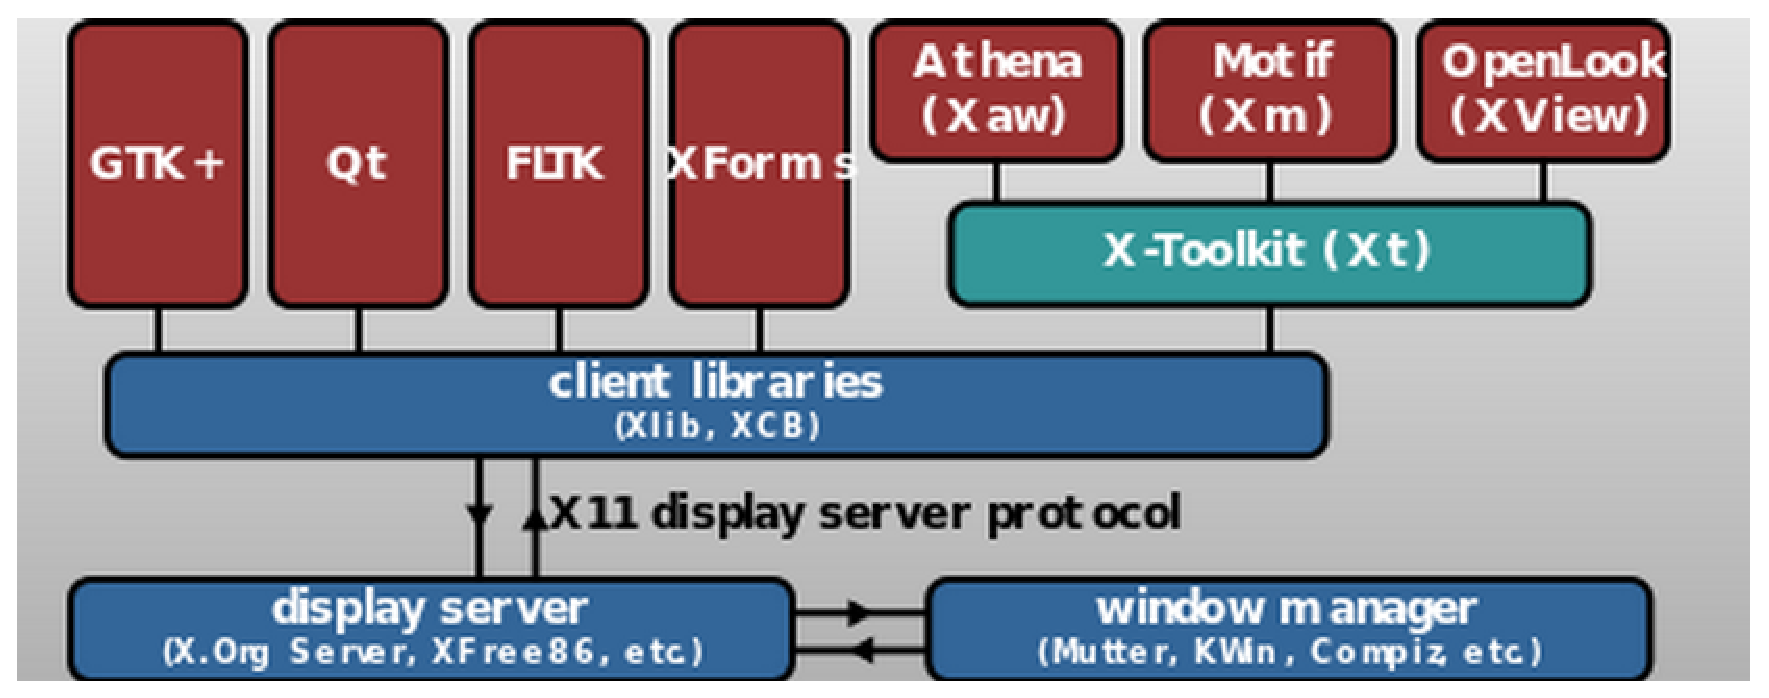
\includegraphics[height=5cm,
    angle=0]{./images/widget_library_system.eps}}
\caption{The hierachy structure of widget toolkits (X aw - Sect.\ref{sec:Xaw}, 
Xm - Sect.\ref{chap:Motif}, GTK+ - Sect.\ref{sec:GTK+},
Qt - Sect.\ref{sec:Qt}, FLTK - Sect.\ref{sec:FLTK}, XForms - Sect.\ref{sec:Forms_Library}),
XView - Sect.\ref{sec:XView}}
\label{fig:widget_library_system}
\end{figure}

\section{Widget Toolkits}
\label{sec:widget-toolkits-list}

A history is covered in Sect.\ref{sec:history-widget-toolkits}

\subsection{GUI Toolkits for C language}

\begin{enumerate}
  \item GTK - Chap.\ref{sec:GTK}
  \item Motif - Chap.\ref{chap:Motif}
  \item LessTif - Chap.\ref{chap:Motif}
\end{enumerate}

\subsection{GUI Toolkits for C++ language}

\begin{enumerate}
  \item GLUI - Sect.\ref{sec:glui}
  \item Qt - Chap.\ref{chap:Qt}
  \item Fox
  \item GTKmm - Sect.\ref{sec:GTKmm}
  \item FLTK - Sect.\ref{sec:FLTK}
  \item TCL/TK
  \item wxWidgets - Sect.\ref{sec:wxWidgets}
\end{enumerate}
\url{http://bwachter.lart.info/documentation/guitoolkits.html}

C++ in Windows
\begin{itemize}
  \item MFC (Sect.\ref{sec:MFC})
\end{itemize}

\subsection{GUI Toolkit for Python language}

\begin{enumerate}
  \item wxPython
  \item Tinker
  \item \ldots
\end{enumerate}
More information: Chap.\ref{chap:UI_Python}.

\subsection{GUI Toolkit for .NET languages (C\#)}

\begin{enumerate}
  \item WinForms: Sect.\ref{sec:Winform}
  \item WPF: from .NET 3.0
\end{enumerate}

\subsection{GUI Toolkits for Java}

\begin{enumerate}
  \item AWT
  \item Swing: more feature than AWT, native look-and-feel, and with the option
  of using a plugable look-and-feel defined by users (i.e. unrelated to
  the underlying platform) (Sect.\ref{sec:look_and_feel_plugable})
  
  
\end{enumerate}

\section{GUI builders}

GUI builders are software that help creating user interface easily (via using
drag-and-drop of mouse). The output is saved in some form of XML format (e.g.
XAML), and during the compilation, the builder will convert to source code of
the appropriate language and then regular compiler will compile to binary code.

\url{http://en.wikipedia.org/wiki/Graphical_user_interface_builder}


\section{Vector-graphics libraries}


\begin{enumerate}
  \item Cairo
\end{enumerate}

\section{Bitmap graphics libraries}

\begin{enumerate}
  \item ImageMagick
\end{enumerate}
\url{http://stackoverflow.com/questions/2650345/imagemagick-vs-cairo-on-vector-graphics-rasterization}

\section{Design Languages}

Design language (design vocabulary) refers to a style that guides the design of
a complements of products to give a consistent look and feel. There are
different choices: materials, colour schemes, shapes, patterns, textures, or
layouts. 

In automobiles, the design language is often in the grille design.
In software architecture, design languages are related to architecture
description languages. The most well-known design language is UML. Others design
language in software
\begin{enumerate}
  \item Material Design (Sect.\ref{sec:MaterialDesign})
  \item Microsoft Metro design language (Sect.\ref{sec:Microsoft_Metro})
  \item Snow White design language (Sect.\ref{sec:SnowWhite})
\end{enumerate}

\subsection{Microsoft Metro}
\label{sec:Microsoft_Metro}

{\bf Metro} is a typography-based design language. The key design is focusing on
the content of applications, relying more on typography (emphasizes
cleanliness, readability and objectivity) rather than the graphics. 

Metro is being used in Windows 8. Early response to the language was generally
positive, but become negative with Windows 8 as it's frustrating and various
aspects of the UI did not work well together. Also, full-screens apps are being
used as thus Microsoft has shift the focus away from multi-tasking and business
productivity.

\subsection{Snow White}
\label{sec:SnowWhite}

The scheme has vertical and horizontal stripes for decoration and it is being
used in many Apple computer from 1984 to 1990. This is for hardware, but not for
software.
\url{http://en.wikipedia.org/wiki/Snow_White_design_language}

\subsection{Material Design}
\label{sec:MaterialDesign}

{\bf Material Design} is a cleaner design that uses grid-based layouts,
with a lot of responsive animations and transitions, padding and depth effects
(e.g. lighting and shadows). Every time we press, there is always a responsive
animation effect. Material Design is built around the idea of
treating the virtual space within your smartphone as if it were a physical object. "What if pixels
didn't just have color, but also depth?" said Google's VP of Design Matias
Duarte.
\footnote{\url{http://www.npr.org/blogs/alltechconsidered/2014/11/16/364152727/googles-lollipop-wants-to-change-the-way-we-use-our-phones}}
\url{http://android-developers.blogspot.com/2014/10/implementing-material-design-in-your.html}

Material Design is used in Android 5.0 (Lollipop). The API for third-party
development to incorporate the design into their applications is 
\url{http://www.google.com/design/spec/material-design/introduction.html}

\url{http://bgr.com/2014/07/30/google-drive-material-design-update/}

It shoulds provide a consistent UI for different platform and device sizes. 
Mobile precepts are fundamental, but touch, voice, mouse, and keyboard are all
first-class input methods.

In material design, UIs are composed of pieces of digital paper \& ink. 
The surfaces and the shadows they cast provide visual cues to the structure of
the application, what you can touch and how it will move. This digital material can move, expand and reform to create flexible UIs.

A material is based on the concept of paper and the content is just like ink
(adding no additional thickness). A material environemt is a 3D space (with
x,y,z dimensions). The z-axis aligns with the plane of the display, with
positive z-axis extending towards the viewer. So, every sheet of material
occupies a single position along the z-axis with a standard 1.0dp thickness; and
with different x- and y- dimentions. Content does not add thickness to material.

Depending on the direction of the virtual light source, a material can cast
shadow on another one. There are two types of light sources:
\begin{itemize}
  \item key light : the first and usually the most important light that a
  photographer (cinematographer, lighting camerman, \ldots) uses in a lighting
  setup.
  \url{http://en.wikipedia.org/wiki/Key_light}
  
  \item ambient light : usually refers to sources of light that are already
  available naturally, not explicitly supplied by the photographer for the
  purpose of taking the photos
\end{itemize}
A key light creates directional shadows, while an ambient light creates
consistent, soft shadows from all angles.
All shadows in the material environment are cast by these two light sources.
Shadows are the absence of light resulting from the occlusion of these light
sources by sheets of material at various positions along the z-axis.

Content behavior can be decoupled from the behavior of material. However, the
bounds of the material can limit the display of the content. It means that if
the material is rezied, the content keep unchanged until we resize the content. 


Material cannot pass through other material. For example, one sheet of material
cannot pass through another sheet of material when changing elevation. This maps
exactly the same in real-world. In the physical world, objects can be stacked or
affixed to one another, but cannot pass through one another

Transforming material
\begin{enumerate}
  \item change shape
  \item grow/shrink along only its plane
  \item never bends or folds (i.e. always on a single z-plane)
  \item Sheets of material can join together to become a single sheet of
  material.
  \item When split, material can heal. For example, if you remove a portion of
  material from a sheet of material, the sheet of material will become a whole sheet again.
  \item can move along any axis.
  
  Z-axis motion is typically a result of user interaction with material.
  Elevation is the relative value between parent and child objects.
  Elevation is measured in the same units as the x and y axes, typically in
  density independent pixels (dps). Since material has a standard 1dp thickness,
  all elevation distances are measured from one top surface to another top surface. 
  
  All material objects have a resting elevation, whether the object is a small
  component or a sheet that spans the entire display. If an object changes
  elevation, it should return to its resting elevation as soon as possible.
  The resting elevation for a given UI component type is consistent across apps
  throughout a platform. However, that same component type may have different
  resting elevations from platform to platform depending on the depth of the
  environment (e.g., TV has a greater depth than mobile or desktop).  
  
  \item Material can be spontaneously generated or destroyed anywhere in the
  environment.
\end{enumerate}

Objects can move independently of each other, or their movement can be
constrained to, and dependent upon, their container. Containers and the objects
they contain have a parent-child relationship. Every object has a single parent,
and may or may not have one or more children.  

\section{VCL (Visual Component Library)}
\label{sec:VCL}

VCL is the visual component-based object-oriented framework, written in Object
Pascal, and is used to develop GUI for Windows applications.
VCL forms a class hierarchy with a common ancestor, i.e. the root base-class
\verb!TComponent! class which inherits from the root class \verb!TObject! in
Delphi Object Pascal. This is utilized in Java, Smalltalk, C\#, etc.
\begin{itemize}
  \item TForm class: windows
  \item TButton, TCheckBox, TLabel classes: controls
  \item database access: 
  \item Internet connections: 
\end{itemize}

VCL supports multithreading, even though not all VCL components are thread-safe. 

\section{.NET}

.NET is good for

\section{Winform}
\label{sec:Winform}

Winform is very much easy. Much of its design is based on VCL
(Sect.\ref{sec:VCL}).

More details: Chap.\ref{chap:Windows.Forms}

Application that use: TortoiseSVN

\section{Qt}
\label{sec:Qt}

Qt used a thing called {\bf MOC} (Meta Object Compiler) which was designed for reflection. 
Qt invented the signal and slot system using in Boost and GTK. Thus, Qt is an event-based GUI framework.

When a user clicks a button it'd send a message (signal) and whatever slot was
connected to the signal would get that event and respond however to it. It is
type safe, you don't have to worry about it messing up. It will just not call
the invalid slot and will report the error letting you know.


Qt has a designer application {\bf Qt-Creator} that allows you to create signals
in it, wide range of widgets to use.
You can even make a widget plugin and put your own widgets in to designer and
drag them on to the form and see it in real time.
You can see the code it generates (via MOC) and spits out 100\% valid C++.

Qt ships with a lot of modules in it. Ranging from SQL, network, XML,
XSLT/XPath, to WebKit. Even COM support (which only runs on Windows).

 QtActive, you can make Qt plugins for Internet Explorer if you want
 
  QtScript, which allows you to add scripting to your application via JavaScript if you would like to have i


  
\section{UI Data binding}
\label{sec:data-binding-UI}


{\bf UI data binding}
\footnote{\url{http://en.wikipedia.org/wiki/UI_data_binding}} is a software
design pattern to simplify the development of GUI application. Each UI element
can bind to an application domain model
(Sect.\ref{sec:software-dev-practices}), Fig.\ref{fig:UI-databinding}.
\footnote{\url{http://msdn.microsoft.com/en-us/library/wxt2cwcc.aspx}}

Once there is a change in the datasource, the UI controls on the GUI form should
be able to get updated. The datasource can be the traditional data sources (e.g.
relational database) or can come in the form of any structures that contains
data (e.g. databases, web services, and objects). Depending on the GUI packages
(e.g. WinForms, WPF, Unity, \ldots), different UI data binding techniques are
supported.


\begin{figure}[hbt]
  \centerline{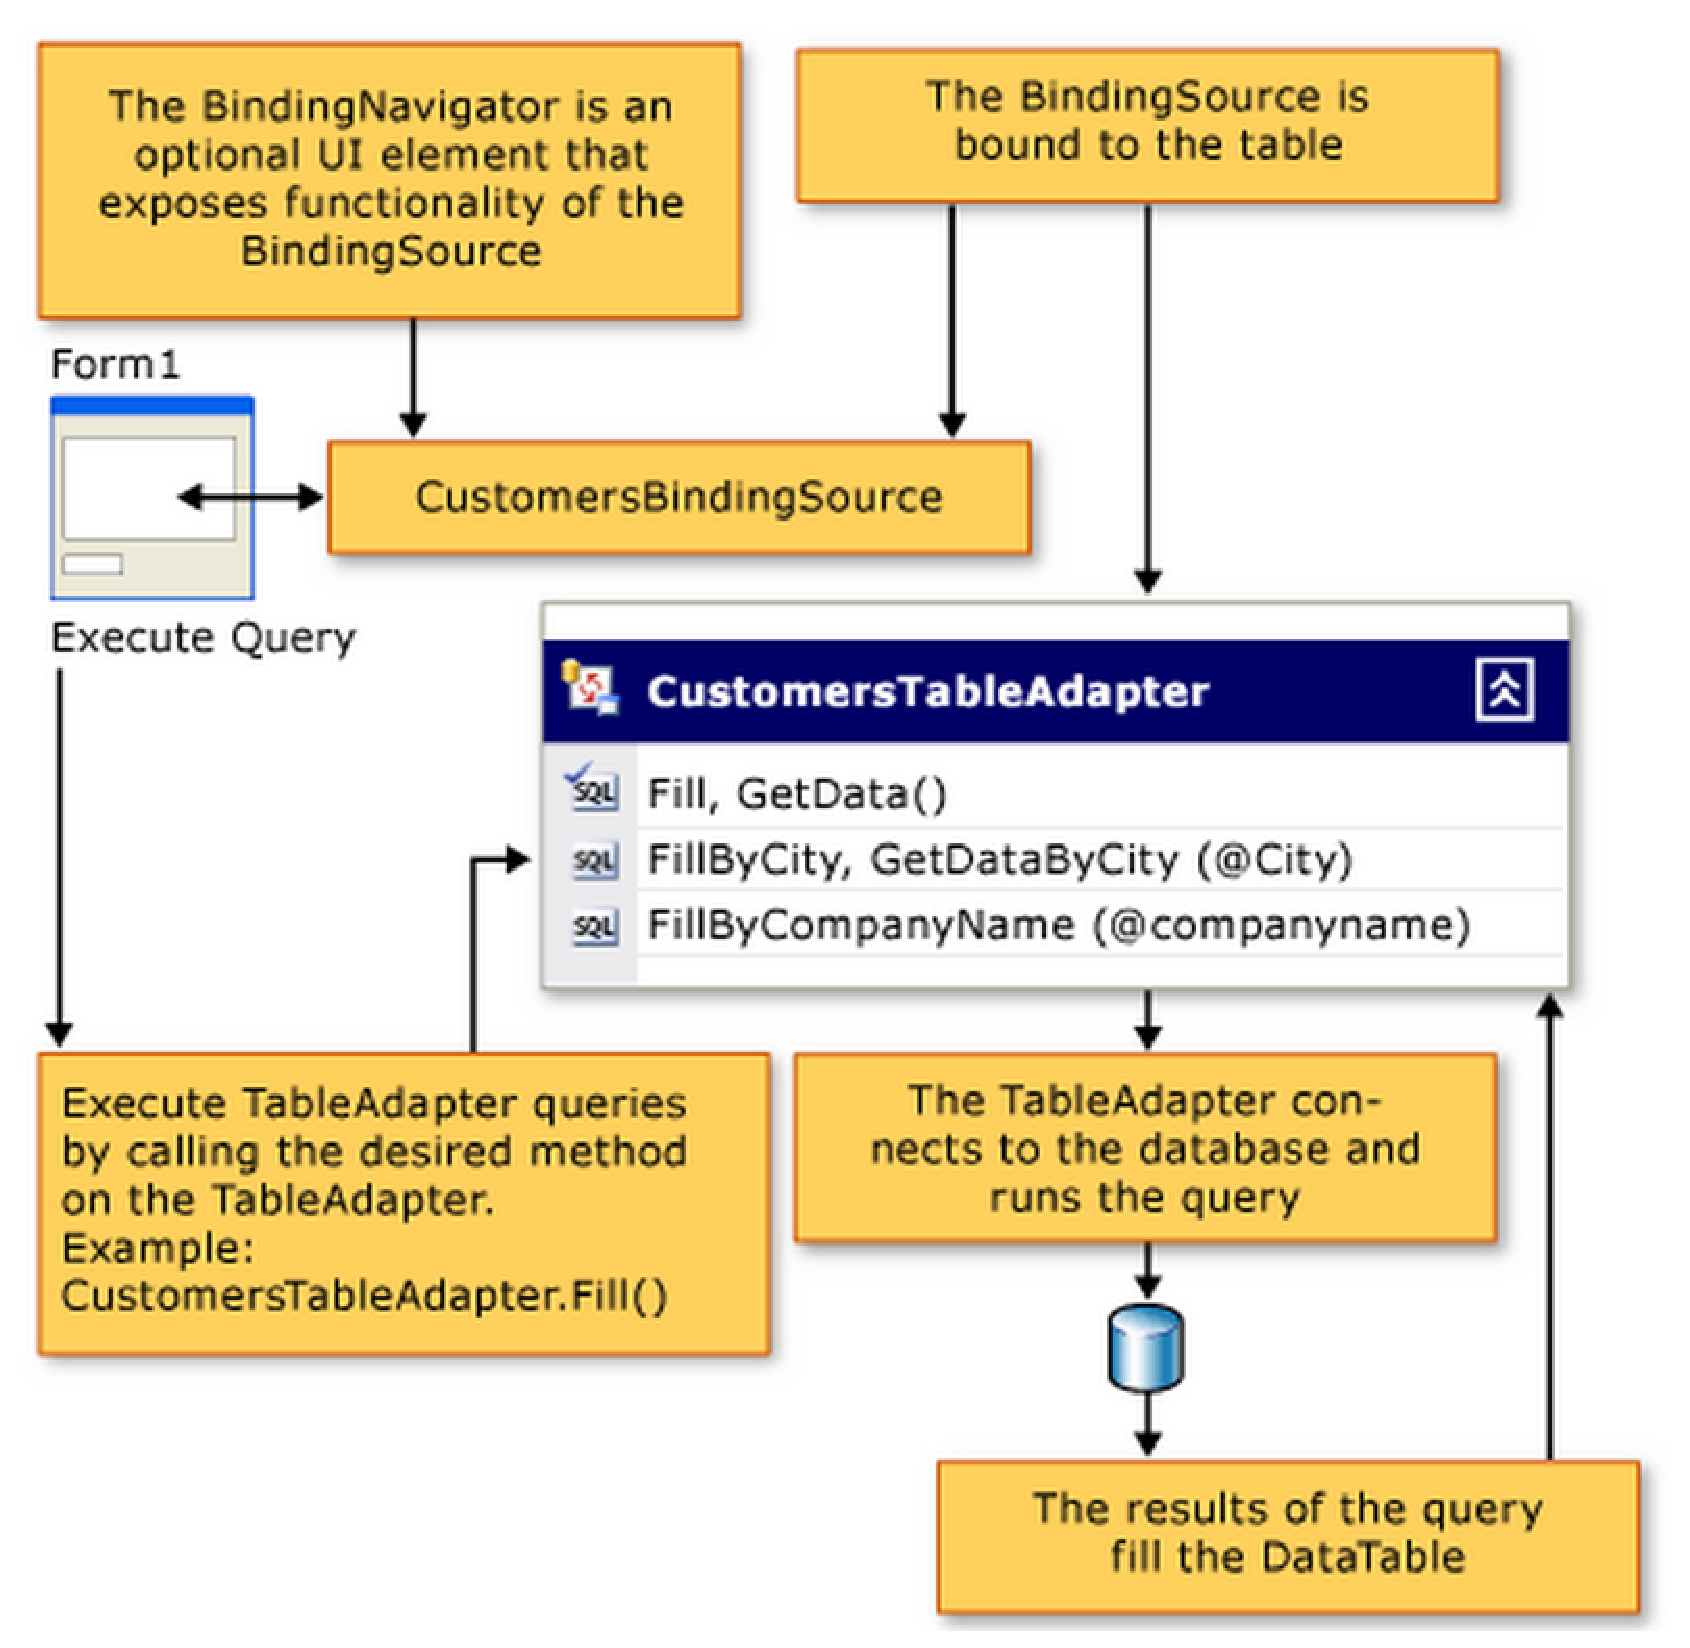
\includegraphics[height=5cm,
    angle=0]{./images/UI-databinding.eps}}
  \caption{UI-databinding}
\label{fig:UI-databinding}
\end{figure}


\section{Software Development Practices}
\label{sec:software-dev-practices}


In UML, a class diagram is used to represent a {\bf Domain
Model}\footnote{\url{http://en.wikipedia.org/wiki/Domain_model}}.
The Domain Model is one of the central parts in FDD (Sect.\ref{sec:FDD}).

\subsection{FDD (Feature-Driven Development)}
\label{sec:FDD}

FDD emphasizes on the progress made for each feature. A feature is a relatively
small task. FDD defines 6 milestones per feature that are to be completed
sequentially. The first 3 are completed during {\bf Design by Feature} activity;
and the last 3 are done during {\bf Build by Feature} activity.
\footnote{\url{http://en.wikipedia.org/wiki/Feature-driven_development}}

Each milestone has a percentable complete value assigned to help tracking the
progress. Example: a feature still being coded with 44\% complete can have
(Domain Walkthrough 1\%, Design 40\% and Design Inspection 3\% = 44\%).

\begin{enumerate}
  \item {\bf Domain Object Modeling}: after explore and explain the domain of
  the problem to be solved; this provdies an overall framework in which new
  features can be added.
  
  \item {\bf Developing by Feature}: any function too complex to be implemented
  within 2 weeks is further decomposed into smaller functions until each
  sub-problem is small enough to be called a {\it feature}. 
  
  Features in this respect were small pieces of client-valued functions
  expressed in the form \verb!<action> <result> <object>!, for example:
  'Calculate the total of a sale' or 'Validate the password of a user'.
  
  This makes it easier to deliver a correct function and to extend/modify the
  system. After the feature list had been completed, the next step was to
  produce the development plan. 
  
  \item {\bf Individual Class (code) Ownership}: distinct pieces or grouping of
  codes are assigned to a single owner. The owner is responsible for the
  consistency, performance, and conceptual integrity of the class.
  
  Class ownership has been done by ordering and assigning features (or feature
  sets) as classes to chief programmers.
  
  \item {\bf Design by Feature}: 
  the chief programmer worked out detailed sequence diagrams for each feature
  and refines the overall model. Next, the class and method prologues are written and finally a design inspection is held.
  
  \item {\bf Buid by Feature}: After a successful design inspection a per
  feature activity to produce a completed client-valued function (feature) is
  being produced. The class owners develop the actual code for their classes. 
  
  
  After a unit test and a successful code inspection, the completed feature is
   promoted to the main build.
  
  
\end{enumerate}

\section{FLTK (Fast Light Toolkit)}
\label{sec:FLTK}

FLTK (``fulltick'') is a light-weight cross-platform GUI toolkit for
UNIX/Linux(X11)/Windows/MacOS X. It was designed to be compatible with
{\bf Forms Library} (Sect.\ref{sec:Forms_Library}). So all functions of FLTK are
also prefixed with \verb!fl_!. 

FLTK is LGPLv2 licensed, with exception ``allow for static linking''. 

FLTK was designed to be statically linked. It is also designed so that all data
used by the GUI, such as images and widget layout, can be inlined into source code.


A GUI Design IDE for FLTK is called FLUID (Fast Light User Interface Designer).
The FLUID program (which includes every widget) is only 352k. 
The output of FLUID is a \verb!*.fl! file and can also be converted to C++
source code and header file.
\url{http://www.fltk.org/documentation.php/doc-1.1/fluid.html}

\subsection{version}

FLTK 1.3:
\begin{verbatim}
svn co http://seriss.com/public/fltk/fltk/branches/branch-1.3/ fltk-1.3

cd fltk-1.3 
// to update
svn update
\end{verbatim}


\subsection{compile fltk in Ubuntu 16.04 on Debian 8 (i.e. Ubuntu 14.04)}
\label{sec:fltk-1.3+-Ubuntu-14.04}

\begin{verbatim}
sudo apt-get build-dep -y libfltk1.3
sudo apt install -y cmake

$ mkdir fltk
$ cd fltk
$ URL=http://archive.ubuntu.com/ubuntu/pool/universe/f/
$ wget ${URL}/fltk1.3/fltk1.3_1.3.3.orig.tar.gz
$ wget ${URL}/fltk1.3/fltk1.3_1.3.3-8.dsc
$ wget ${URL}/fltk1.3/fltk1.3_1.3.3-8.debian.tar.xz
$ tar zxvf fltk1.3_1.3.3.orig.tar.gz
$ cd fltk-1.3.3/
$ tar xvf ../fltk1.3_1.3.3-8.debian.tar.xz

//build
dpkg-buildpackage -us -uc

//now we can install
$ cd ..
$ sudo dpkg -i *.deb || (sudo apt -f install -y ; sudo dpkg -i *.deb)
$ cd ..
\end{verbatim}



\subsection{compile fltk from source}
\label{sec:fltk-compile}

NOTE: FLTK 1.3+ requires libpng 1.4+ (Sect.\ref{sec:libpng}), as it uses
\begin{verbatim}
The "png_set_longjmp_fn()" API was introduced in libpng-1.4.x. Ubuntu 13:10
currently comes with libpng-1.2.49 (see /usr/include/libpng12), which does not
supply png_set_longjmp_fn(). 
\end{verbatim}
\url{https://stackoverflow.com/questions/21545076/libpng-png-set-longjmp-fn-not-found}

We need to update \verb!CMAKE_CXX_FLAGS! to get proper link to the library
\begin{verbatim}
rm * -rf ; cmake -DCMAKE_INSTALL_PREFIX:PATH=/packages/fltk/1.3/
 -DCMAKE_PREFIX_PATH=/packages/libpng/1.5 -DCMAKE_REQUIRED_LIBRARIES=-lpng
 -DCMAKE_REQUIRED_INCLUDES=/packages/libpng/1.5/include
 -DCMAKE_CXX_FLAGS="-I/packages/libpng/1.5/include -L/packages/libpng/1.5/lib -lpng" \
 ../; make -j4 
\end{verbatim}

If the fltk library is installed via Cmake, it will create these files
\begin{verbatim}
/packages/fltk/1.3/share/fltk/FLTK-Functions.cmake
/packages/fltk/1.3/share/fltk/FLTK-Targets-noconfig.cmake
/packages/fltk/1.3/share/fltk/FLTKConfig.cmake
/packages/fltk/1.3/share/fltk/UseFLTK.cmake
/packages/fltk/1.3/share/fltk/FLTK-Targets.cmake
\end{verbatim}

\subsection{writing GUI using FLTK}

IMPORTANT:
\begin{verbatim}
#include <fltk/Window.h>
#include <fltk/Widget.h>
#include <fltk/run.h>
using namespace fltk;
\end{verbatim}

Then, we create a window of class \verb!Window!, add as many widgets as you
want, and show the window
\begin{verbatim}
int main(int argc, char **argv) {
  Window *window = new Window(300, 180);
  window->begin();
  Widget *box = new Widget(20, 40, 260, 100, "Hello, World!");
  box->box(UP_BOX);
  box->labelfont(HELVETICA_BOLD_ITALIC);
  box->labelsize(36);
  box->labeltype(SHADOW_LABEL);
  window->end();
  window->show(argc, argv);
  return run();
}
\end{verbatim}

To compile your code
\begin{verbatim}
g++ `fltk-config --cxxflags` snippet.cpp `fltk-config --libs` -lX11 -ldl -lXext
-lXinerama -lXft -lfontconfig -o snippet
\end{verbatim}
NOTE: \verb!fltk-config! (with the flag \verb!--libs! for linker, and
\verb!--cxxflags! for header file) can be used to produce a set of flags to pass
to your gcc.


\section{Forms Library and XForms}
\label{sec:Forms_Library}

Forms Library is written for SGI machines. Its derivative is XForms

In Forms Library, all functions are prefixed with \verb!fl_!.


\section{MFC}
\label{sec:MFC}

MFC is thinnest layer over Win32, GUI, controls, DLL, file IO, multithreading etc.
It is thin layer over socket, networking, internet programming.
And it facilitates COM programming with thickest layer.

MFC use {\bf message maps} (Sect.\ref{sec:message_map}) as an alternative to the
switch statement used in traditional Windows programs to handle messages sent to
a window.

\url{https://wiki.wxwidgets.org/WxWidgets_Compared_To_Other_Toolkits}

\subsection{message map}
\label{sec:message_map}

Message Maps maps the user action into the appropriate MFC class functions to handle it. 
A mapping from messages to member-functions may be defined so that when a
message is to be handled by a window, the appropriate member function is called
automatically.

The advantage of Message Map is the same action can be mapped to more than one
MFC class function.
This message-map facility is designed to be similar to virtual functions but has
additional benefits not possible with C++ virtual functions.

The MFC Class which can handle message should be member of CCmdTarget, (i.e.) it
should be hierarchically derived from CCmdTarget.

To do the mapping, MFC define a macro \verb!DECLARE_MESSAGE_MAP!. A Class wizard can help you to create a class
\begin{verbatim}
class CMyWnd : public CMyParentWndClass
{
    // my stuff...

protected:
    //{{AFX_MSG(CMyWnd)
    afx_msg void OnPaint();
    //}}AFX_MSG

    DECLARE_MESSAGE_MAP()
};
\end{verbatim}
that automatically add \verb!//{{! and \verb!//}}! brackets.

\url{https://msdn.microsoft.com/en-us/library/aa267978.aspx}


\section{Event-driven app}
\label{sec:event_driven_app}

In an event-driven application, there is generally a main loop that listens for
events, and then triggers a callback function when one of those events is
detected. Event-driven programming is widely used in GUI apps.

\begin{mdframed}
In embedded systems the same may be achieved using hardware interrupts instead
of a constantly running main loop.
\end{mdframed}


The first step in developing an event-driven program is to write a series of
subroutines, or methods, called event-handler routines (or {\it callback
function} - a term in Windows).

\url{http://en.wikipedia.org/wiki/Event-driven_programming}


\section{DirectX}
\label{sec:DirectX}

Microsoft DirectX is a collection of APIs for handling
tasks related to multimedia, especially game programming and video, on
Microsoft platforms.
Originally, they are separated libraries: 
Direct3D, DirectDraw, DirectMusic, DirectPlay, DirectSound, \ldots
The name DirectX was coined as shorthand term for all of these APIs.

DirectX 1.0 is the replacement for WinG APIs (Sect.\ref{sec:WinG}) when
switching from Windows 3.1 to Windows 95. Like WinG, DirectX 1.0 was designed to
enable direct access to hardware devices (video cards, keyboards, mice, sound
devices).
\begin{itemize}
  \item DirectX 8.0 is the last version to have software rendering support.

  \item DirectX 9.0c RC0 is the first to have 64-bit capable build.
\end{itemize}

DirectX includes APIs not only for GUI, but also for multimedia processing
(DirectMusic, DirectPlay, DirectSound).
Here we introduce APis for GUI
\begin{enumerate}
  \item DirectDraw : until DirectX 8.0, then merged into Direct3D
  \item Direct3D: added since DirectX 3.0 version number 4.04.00.0069
  
Direct3D (Sect.\ref{sec:Direct3D}) however, focused on game use.  
\end{enumerate}

\section{Java-based libraries}

native rendering libraries with Java APIs 
\begin{enumerate}
  \item Mophun
  by  Synergenix,  
  
  \item Brew
  by  Qualcomm  and
  
  \item JBlend by  Aplix
\end{enumerate}

Typically,  Java-Based  Graphic  APIs  such  as  
Brew  or  JBlend  only  work  on  mobile  phones,  making  it  difficult  
to target other devices such as handheld computers using the same 
code  base.



\section{Desktop Environment}
\label{sec:desktop_environment}

\begin{verbatim}
>> echo $DESKTOP_SESSION

gnome


>> ps -ef | grep gnome

>> ps -A | egrep -i "gnome|kde|mate|cinnamon|lxde|xfce|jwm"
\end{verbatim}

\subsection{GNOME}

Sect.\ref{sec:GNOME} in 'GUI development' book discusses in depth.

GNOME2 used Metacity window manager (Sect.\ref{sec:Metacity}).

GNOME3 used Mutter window manager (Sect.\ref{sec:Mutter}). 

\subsection{Unity}
\label{sec:Unity}

Unity was first developed by Canonical to replace GNOME 2. However, after 7
years, Canonical now switched back to GNOME 3 in Ubuntu 18.04.

It has a bar at the top which contains the clock at the right and a button on
the left which will bring up a search/menu window. There's a launcher on the
left of the screen. The default theme color is purple/orange/brown.

\subsection{MATE}
\label{sec:MATE}

MATE is a fork of Gnome 2. It features two bars, one on the top of the screen,
one at the bottom. 
\begin{enumerate}
  \item  The top one contains the main menu (dropdown with three items,
  Applications, Places and System), some starters and the clock on the far right. 
  
  \item The lower bar holds the window list and the desktop switcher.
\end{enumerate}
MATE also has icons (Computer, Home, Trash and also removable media) on the
desktop in the default configuration.

\subsection{XFCE}
\label{sec:XCFE}

XFCE is very similar to MATE/Gnome 2 and might easily be confused with the two.
The default configuration is similar to MATE/Gnome 2 except that the menu in the
upper bar is only an icon, but is similarly structured.

\subsection{KDE}
\label{sec:KDE}

KDE is one of the oldest desktop environments. It features a bar at the bottom
of the screen which contains the main menu (as icon), the window list and a
clock. The main menu is a big dropup menu sorted in categories. 

\subsection{Cinnamon}
\label{sec:Cinnamon}

Cinnamon is heavily based on Gnome 3. It features a lower bar similar to KDE, as
it contains the menu button, the window list and the clock.




\section{Window Manager}
\label{sec:window_manager}

\url{http://en.wikipedia.org/wiki/Comparison_of_X_window_managers}

To ensure different window managers provide a consistent interface for the
applications to interact, a window manager should be designed following NetWM
(or EWMH - {\it Extended Window Manager Hints}) standards
\url{http://blackboxwm.sourceforge.net/NetWM}.
The older version of NetWM is called ICCCM (Inter-Client Communications
Conventions Manual) - Sect.\ref{sec:ICCCM}.

\subsection{ICCCM}
\label{sec:ICCCM}
\label{sec:selections}
\url{https://tronche.com/gui/x/icccm/}

\begin{mdframed}
In X10, "cut buffers" were introduced. These were limited buffers that stored
arbitrary text and were used by most applications.  Cut buffers are long
deprecated, and although some applications (such as xterm) may have legacy
support for them, it is both not likely and not recommended that they be used.  

In the old "cut buffers" system where arbitrary applications could modify data
stored in the cut buffers. In ICCM, only one application may control or "own" a
selection at one time. So, when that application is closed, the selection text
is lost.
\end{mdframed}

\begin{itemize}
  \item ICCM version 2.0  is standardized in X11R6 (Sect.\ref{sec:X11R6})
\end{itemize}

{\bf Selections} are the primary mechanism that X Version 11 defines for the
exchange of information between clients, for example, by cutting and pasting
between windows.

There can be an arbitrary number of selections (each named by an atom) and that
they are global to the server. 
\url{https://tronche.com/gui/x/icccm/sec-2.html}

To conform with the inter-client conventions, however, clients need deal with
only these three selections, named by the atom  
\begin{enumerate}
  \item PRIMARY
  
  used by the commands that take only a single argument and is the principal
  means of communication between clients that use the selection mechanism. 
  
  \item SECONDARY
  
  used as (1) the second argument to commands taking two arguments; 
  (2)  a means of obtaining data when there is a primary selection and the user
  does not want to disturb it 
  \item CLIPBOARD
  
  used to hold data that is being transferred between clients, that is, data
  that usually is being cut or copied, and then pasted
\end{enumerate}
respectively.\footnote{\url{https://tronche.com/gui/x/icccm/sec-2.html\#s-2.6}}

Of the three selections, users should only be concerned with PRIMARY and
CLIPBOARD.   
\begin{itemize}
  
  \item The CLIPBOARD selection is accessed using keyboard shortcuts, while
application specific, these are most commonly ctrl+c for copying, ctrl+v for
pasting and ctlr+x for cutting.

The clipboard may also contain other items than text, such as images or folders.

  \item  The PRIMARY selection speeds up the copying task by copying the text to
  the clipboard as soon as it was selected with the mouse, without the need for
  entering a keyboard shortcut.  
  
   Pasting is triggered by pressing the middle mouse button (or some emulation
   of it). 
\end{itemize}
\url{https://wiki.archlinux.org/index.php/Clipboard\#List_of_clipboard_managers}

Other selections may be used freely for private communication among related
groups of clients. 

Let's discuss some application's behavior with the PRIMARY selection and
CLIPBOARD selection
\begin{enumerate}
  \item gvim with \verb!+clipboard! feature
  
  \verb!*! register represents the PRIMARY buffer in X.
  
  vim's command \verb!:yank! (or yank selected text with yy; or yank current
  work with yw; or yank current character with yc) and \verb!:paste! 
 operate on unnamed register, which by default corresponds to \verb!*! register.
 
  
  \item the list of clipboard managers
  
\begin{verbatim}
Xclip - A lightweight, command-line based interface to the clipboard.

Autocutsel - Command line and daemon interfaces to synchronize 
             PRIMARY, CLIPBOARD and cut buffer selections.
 
\end{verbatim}
  \url{https://wiki.archlinux.org/index.php/Clipboard\#List_of_clipboard_managers}
\end{enumerate}



\subsection{Blackbox}

Blackbox is the fast, lightweight window manager for the X Window System
(version 6+).
lackbox is built with C++ and contains completely original code (even though the
graphics implementation is similar to that of WindowMaker or NeXT interface).
\begin{itemize}
  \item The first stable Blackbox release (0.51.3.1) was built from only 14,406
  lines of code (includes source, headers, comments and preprocessor
  statements). The latest version has around 40,000 lines. 
  
\end{itemize}

Blackbox itself does not directly handle key bindings like  most  other
window  managers.  This  task  is  handled by a separate utility called
\verb!bbkeys!.
The slit is an edge of the screen which  can  hold  specially  designed
        programs  called dock apps (from Windowmaker). In addition, the popular
        program gkrellm will also run in the slit.  There is a  huge  selection
        of  dockapps available and they run the gamut from must-have gadgets to
        utterly useless (but cute and/or funny) eye candy. 

\subsection{WindowMaker}
\label{sec:WindowMaker}

\subsection{evilwm}

evilwm is a minimalist window manager for the X Window System. It maximises
screen real estate and provides good keyboard control. It is currently based on
aewm. 

\subsection{Metacity}
\label{sec:Metacity}

Metacity is used by these desktop environments:
\begin{itemize}
  \item GNOME2
  \item GNOME Flashback
\end{itemize} 

Metacity used GTK+ graphical widget toolkit to create the UI components
\begin{itemize}
  \item Metacity older version: GTK+ 2
  \item Metacity 3.12.0+: use GTK+ 3
\end{itemize}

Its fork:
\begin{itemize}
  \item Marco: 
\end{itemize}

\subsection{Mutter}
\label{sec:Mutter}

Mutter is a window manager (Sect.\ref{sec:window_manager}) that uses Clutter
graphics library (Sect.\ref{sec:Clutter}), instead of GTK+ for
rendering (Sect.\ref{sec:GTK+}). Mutter is a replacement for Metacity, i.e. the
name coming from Metacity and Clutter. Clutter also support OpenGL.

The Mutter window manager can function as a standalone window manager
application for GNOME-like desktops, and serves as the primary window manager
for the GNOME Shell desktop. GNOME Shell is implemented as a plugin to Mutter.


Mutter is a GObject-based library for creating compositing window managers.
Compositors that wish to use Mutter must implement a subclass of MetaPlugin and
register it with \verb!meta_plugin_manager_set_plugin_type()! before calling
\verb!meta_init()! but after \verb!g_type_init()!. 

MetaPlugin class is the entry point for plugins.
MetaPlugin provides virtual functions that allow to override default behavior in
the window management code, such as the effect to perform when a window is
created or when switching workspaces. 

Mutter automatically checks environment variables during its initialization.
These environment variables are meant as debug tools or overrides for default
behaviours, e.g. \verb!MUTTER_DISPLAY! (name of X11 display to use)
\url{https://developer.gnome.org/meta/stable/running-mutter.html}



\subsection{Gala}

Gala is the window manager based on Mutter (Sect.\ref{sec:Mutter}).

\section{X Display Managers}
\label{sec:Display_manager}

A display manager, sometimes  referred to as a ``login manager'', presents the
user with a login screen. A session starts when a user successfully enters a
valid combination of username and password.

A display manager is responsible for starting the display server (Wayland
compositor - Sect.\ref{sec:Wayland}, Mir - Sect.\ref{sec:Mir}, X.org -
Sect.\ref{sec:X.org}) and loading the window manager (
Sect.\ref{sec:window_manager} such as KWin - Sect.\ref{sec:KWin}), OpenBox -
Sect.\ref{sec:OpenBox}), DWM - Sect.\ref{sec:DWM}) after you type in your
username and password.
All three components interact with each other, but they don't have the same
functionality, so the terms should not be used interchangeably


An X Display Manager control a login session (by loading necessary things so
that a user can interact with the system via a specified session - from the
beginning to until you logout - Sect.\ref{sec:X-session})
\begin{enumerate}
  \item how the login screen look likes
  
  \item how the windows/dialog look likes
\end{enumerate}

NAMES of display managers
\begin{enumerate}
  \item LightDM - Sect.\ref{sec:LightDM} 
  
  It was first introduced in Ubuntu 11.10.
  LightDM was praised as the lightweight alternative to GDM. Apart from X.Org,
  it also supports Canonical's Mir display server.
  LightDM is customizable and featureful, but it doesn't lock you down with a
  bunch of dependencies.
  
   However, Ubuntu is switching to GDM as the default display manager in both
   Ubuntu 17.10 and 18.04 LTS.	
  
  
  \item GDM - Sect.\ref{sec:GDM}, replaced by GDM3
  
  Its name means GNOME Display Manager, i.e. originally designed to start GNOME
  session.
  
  \item GDM3 - Sect.\ref{sec:GDM3}
  \item KDM - Sect.\ref{sec:KDM}, replaced by SDDM

KDM supports both X.Org and Wayland
  
  \item SDDM - Sect.\ref{sec:SDDM}


  \item X-session - Sect.\ref{sec:X-session}
  
  \item MDM - Sect.\ref{sec:MDM} - 
  
MDM was initially based on the "legacy" GDM 2.20 and envisioned as an
alternative to new, redesigned GDM3 for users who wanted the old display manager
back.

\item LXDM - Sect.\ref{sec:LXDM}

LXDM is part of the LXDE environment, and it used to be the default display
manager of Lubuntu until version 12.04. 
\end{enumerate}

The display manager is used to start a desktop environments
(Sect.\ref{sec:desktop_environment}), e.g. GNOME - Sect.\ref{sec:GNOME}.
Currently due to a bug (I checked in 16.04) you cannot start GNOME3 or Ubuntu
Unity session using SDDM.
\url{https://askubuntu.com/questions/829108/what-is-gdm3-kdm-lightdm-how-to-install-and-remove-them}

If you have multiple display managers installed, to switch between them
\begin{verbatim}
//check which is the one being used
cat /etc/X11/default-display-manager


// e.g switch to GDM
sudo dpkg-reconfigure gdm

// e.g. to GDM3
sudo dpkg-reconfigure gdm3
\end{verbatim}

\subsection{LightDM}
\label{sec:LightDM}

LightDM is an X display manager (Sect.\ref{sec:Display_manager}) that aims to be
lightweight, fast, extensible and multi-desktop. 
LightDM does not yet support wayland (Sect.\ref{sec:Wayland}).
\url{https://bugs.launchpad.net/ubuntu/+source/lightdm/+bug/1632772}

Itdoes not load any GNOME
libraries to work. LightDM is Canonical's solution for a display manager. It was
supposed to be lightweight and comes by default with Ubuntu, Xubuntu, and Lubuntu.

It was first used in Ubuntu 11.10, and then until 16.04. Since Ubuntu 17.10, it
switches to using GDM again.

\begin{verbatim}
'
We've attempted to get the GNOME Shell lock screen running with LightDM and
using GNOME Shell as a LightDM Greeter. Which this still seems possible, it's
not easy to patch GNOME Shell as the GDM code is hard to decouple,
' Ancell explains.


'Given the workload we have and the risks in modifying GNOME the decision is to
use GDM for 17.10 and thus 18.04 LTS.'

Ancell adds that Ubuntu will 'continue to support LightDM for the supported
Ubuntu releases' (14.04 LTS, 16.04 LTS and 17.04) and 'for use in the other
flavours'.  
\end{verbatim}


It is used by GNOME 3 Desktop
(Sect.\ref{sec:GNOME-desktop}). LightDM is the display manager running in Ubuntu
up to version 16.04 LTS.


\begin{verbatim}
sudo apt-get install lightdm

// sudo apt-get remove lightdm
\end{verbatim}



LighDM configuration is governed by the configuration files in
\begin{verbatim}
/etc/lightdm/lightdm.conf

/usr/share/lightdm/lightdm.conf.d/*.conf
/etc/lightdm/lightdm.conf.d/*.conf


  // this config file will be ignored if accountsservice is running on your
  // system
  // ps -aef | grep accountsservice
/etc/lightdm/users.conf
\end{verbatim}
To add your own configuration, create a new file in that directory such as
/etc/lightdm/lightdm.conf.d/my.conf.

To display list of users at login, LightDM uses various front-ends to draw login
interfaces, so-called Greeters.
\begin{itemize}
  \item  Unity Greeter (and some other greeters) shows the list of possible user
  accounts by default

\verb!/etc/lightdm/users.conf! file content  
\begin{verbatim}
[SeatDefaults]
greeter-hide-users=true

\end{verbatim}  

background
  
\begin{verbatim}
 /usr/share/glib-2.0/schemas/10_unity_greeter_background.gschema.override
 
[com.canonical.unity-greeter]
draw-user-backgrounds=false
background='/foo/wallpaper.png'
\end{verbatim}
 sudo glib-compile-schemas /usr/share/glib-2.0/schemas/ to apply these settings.
  
  \item LightDM GTK+ greeter
  
\begin{verbatim}
/etc/lightdm/lightdm-gtk-greeter.conf:

background=/usr/share/lubuntu/wallpapers/lubuntu-default-wallpaper.png
\end{verbatim}

  \item lightdm (15.10 onwards) have replaced the obsolete [SeatDefaults] with [Seat:*]
\begin{verbatim}
[SeatDefaults]
user-session=mysession
\end{verbatim}
  

\end{itemize}
\url{https://wiki.ubuntu.com/LightDM}


\subsection{GDM (GNOME Display Manager)}
\label{sec:GDM}

GDM is the display manager (a graphical login program) for the windowing systems
X11 and Wayland. It is a highly configurable reimplementation of XDM
(Sect.\ref{sec:xdm}). 

The X11 window system by default uses the XDM. However, resolving XDM's
configuration issues typically involves editing a configuration file via
command-line. GDM allows users to customize or troubleshoot settings without
having to resort to a command line.

Also, GDM allows you to log into your system with the X Window System running
and supports running several different X sessions on your local machine at the
same time (Sect.\ref{sec:X-session}).

\subsection{GDM3 (GNOME Display Manager)}
\label{sec:GDM3}

GDM3 is a successor of GDM display manager (Sect.\ref{sec:Display_manager}).
The newer gdm3 uses a minimal version of gnome-shell, and provides the same look
and feel of as GNOME3 session. You can install it with:
\begin{verbatim}
sudo apt-get install gdm3

//sudo apt-get remove gdm3


\end{verbatim}


\subsection{XDM (X Display Manager): xdm}
\label{sec:xdm}

\verb!xdm! is the binary of XDM - the X Display Manager.
Now X11 uses GDM (Sect.\ref{sec:GDM}). 


A standard login screen via XDM can be customized using XBanner.
XBanner was invented and designed from the beginning to serve one purpose - to
beautify the login screen XDM usually generates. This beautification is
accomplished by drawing a piece of text in a very large font, then rendering
some graphic effect on the text and/or the screen background.
\url{http://www.linuxjournal.com/article/1357}


\subsection{KDM (KDE Display Manager)}
\label{sec:KDM}


KDM has been deprecated in KDE5 in favor of SDDM (Sect.\ref{sec:SDDM}), which is
more capable as a display manager, and hence comes by default with Kubuntu.

\subsection{SDDM}
\label{sec:SDDM}




\subsection{X-session}
\label{sec:X-session}




\subsection{Troubleshoot login issue}

\begin{verbatim}
Failed to start session
\end{verbatim}
Run
\begin{verbatim}
sudo apt-get install --reinstall lightdm ubuntu-gnome-desktop
\end{verbatim}
Sect.\ref{sec:GNOME-desktop}.




\section{Libraries}


\subsection{libpng}
\label{sec:libpng}

libpng 1.5.4: \url{https://launchpad.net/libpng/main/1.5.14}
\begin{verbatim}

\end{verbatim}

\chapter{Compositing Engines}
\label{sec:compositing_engine}  


A compositing engine combines visual elements from separate source into single
images.
All compositing involves the replacement of selected parts of an image with
other material, usually, but not always, from another image.

\url{http://en.wikipedia.org/wiki/Compositing}

\section{Quartz compositor}
\label{sec:Quartz_compositor}



\section{ Desktop Window Manager}

DWM is the new name for Desktop Compositing Engine or DCE.

\url{http://en.wikipedia.org/wiki/Desktop_Window_Manager}


The Desktop Window Manager is a compositing window manager.
This means that each program has a buffer that it writes data to; DWM then
composites each program's buffer into a final image.
  
  
DWM uses DirectX 9 to perform the function of compositing and rendering in the
GPU, freeing the CPU of the task of managing the rendering from the off-screen
buffers to the display.
However, applications painting to the off-screen buffers - depending on the
technologies used for that, might still be CPU-bound.
  
  
  
\chapter{Desktop App Development}

Traditionally, we use widgets, with APIs provided via C/C++ or Java binding to
write GUI Desktop apps. Nowadays, with the advancement of browsers and mobile
devices, it is shifting to writing mobile and web applications (using
JavaScript), that can run as a regular desktop apps. 

The main idea behind developing desktop applications with JavaScript is that you
build one codebase and package it for each operating system separately, i.e.
write once run everywhere (via the webbrowser). Nowadays, developing a desktop
application with JavaScript relies on either Electron or NW.js.

\section{Using Javascript}

NW.js, Electron provides a platform to write desktop applications with
JavaScript and HTML and has Node integration to grant access to the low level
system from web pages. 

\section{-- NW.js (previously: node-webkit)}

Roger Wang, of Intel's Open Source Technology Center, created \verb!node-webkit!
in 2011. This allowed the user to spawn a WebKit browser window and use Node.js
modules within \verb!<script>! tags.

Soon, it was switched from WebKit to Chromium (the open-source project Google
Chrome is based on), and an intern named Cheng Zhao joined the project. It was
soon realized that an app runtime based on Node.js (Sect.\ref{sec:Node.js}) and
Chromium would make a nice framework for building desktop apps.

\begin{mdframed}
node-webkit was later renamed NW.js to make it a bit more generic because it no
longer used Node.js or WebKit.

NW.js is based on io.js (the Node.js fork) at the time, and Chromium had moved
on from WebKit to its own fork, Blink.

\end{mdframed}

\section{-- Electron (previously: Atom Shell)}

Electron was previously named Atom Shell.


\import*{../Website_Builder/}{JavaScript.tex}  
\import*{../Website_Builder/}{WebBrowser.tex}  
\import*{../Website_Builder/}{ServerSide_Programming.tex}  

\part{OpenGL}

\lstset{language={C}, numbers=left, numberstyle=\tiny,
  stepnumber = 5, numbersep=5pt, keywordstyle=\color{blue}}

\chapter{OpenGL}
\label{chap:opengl}


\section{OpenGL specification}
\label{sec:history-OpenGL}

Brief introduction of OpenGL is given in Sect.\ref{sec:OpenGL}.



\subsection{naming convention}	

The prefix for function is \verb!gl!, the prefix for parameter's value
is \verb!GL_!. The suffix is used to specify the arguments
and data types passed to the functional call. 
\begin{verbatim}
glColor3f(1, 0, 0);         // set rendering color to red 
              //with 3 floating numbers
glColor4d(0, 1, 0, 0.2);    // set color to green with 20% 
              //of opacity (double)
\end{verbatim}
Since OpenGL 1.1, with vertex array, we have a set of new functions,
e.g. \verb!glVertex[size][type]v()!. 
\begin{verbatim}
glVertex3fv(vertex);        // set x-y-z coordinates using
              // pointer
\end{verbatim}

As GPU vendors may provide additional functionality in the form of extensions.
Extensions may introduce new functions and new constants, and may relax or
remove restrictions on existing OpenGL functions.
Each extension is associated with a short {\it identifier}.
\begin{itemize}
  \item  based on the name of the company which developed it, e.g. Nvidia use
  'NV' - e.g. \verb!GL_NV_half_float! constant or \verb!glVertex2hNV()! function.
  
  \item If multiple vendors agree to implement the same functionality using the same
API, a shared extension may be released, using the identifier \verb!EXT!.
  
  \item If Khronos's Architecture Review Board (ARB) gives the extension their
  explicit approval, in which case the identifier \verb!ARB! is used.
\end{itemize}

\subsection{Extensions}
\label{sec:extensions}

Extensions may introduce new functions, new constants, or
add new features to existing functions. Look at the suffix of the
function names or the constants to recognize the Vendor abbreviation, Table~\ref{tab:GL_prefix}

\begin{table}[hbt]
\begin{center}
\caption{OpenGL extension prefix}
\begin{tabular}{cc} 
\hline
\verb!SGI_! &  Silicon Graphics \\
\verb!ATI_! &  ATI Technologies \\
\verb!AMD_! &  Advanced Micro Devices \\
\verb!NV_! &  NVIDIA \\
\verb!IBM_! &  IBM \\
\verb!WGL_! &  Microsoft \\
\verb!EXT_! &  Cross-Vendor \\
\verb!ARB_! &  ARB Approved \\
\hline\hline
\end{tabular}
\end{center}
\label{tab:GL_prefix}
\end{table}
If more than one company agreed to implement the same function, the
default extension is \verb!EXT_!. If the extension become the
standard, the extension becomes \verb!ARB!. This is the final step for
it to become the standard in the future release of OpenGL. 

\begin{verbatim}
glCombinerParameterfvNV()
GL_NORMAL_MAP_NV
\end{verbatim}


\begin{framed}
  Most of the features that are required to perform general
  floating-point computations on the GPU are not part of core
  OpenGL. OpenGL extensions a way to get access to these hardware
  features. 
\end{framed}

\begin{enumerate}
\item Check how many extensions supported?
\begin{verbatim}
GLint nNumExtensions;
glGetIntegerv(GL_NUM_EXTENSIONS, &nNumExtensions);
\end{verbatim}

\item Look for the extension you want, and then get the function
  pointer to the function in that extension
  \begin{enumerate}
  \item Loop through the extension contain that function
\begin{verbatim}
for(GLint i = 0; i< nNumExtensions; i++)
  if(strcmp("WGL_EXT_swap_control", 
          (const char *)glGetStringi(GL_EXTENSIONS, i)) == 0) {
     wglSwapIntervalEXT =
         (PFNWGLSWAPINTERVALEXTPROC)wglGetProcAddress("wglSwapIntervalEXT");

     if(wglSwapIntervalEXT != NULL)    wglSwapIntervalEXT(1);
}

\end{verbatim}
    with \verb!wglGetProcAddress()! is a Window APIs. So, this cannot
    be used in Linux. We can use \verb!glXGetProcAddress()!. 
    
  \item GLTools support this
\begin{verbatim}
int gltIsExtSupported(const char *extension);
\end{verbatim}
which can be used in either Windows or Linux.

    \item Use GLEW which can be use in either Windows or Linux. 

\end{enumerate}

\end{enumerate}

\begin{framed}
  Using OpenGL extensions is important as it allows you to take
  advantages of improve rendering performance and visual quality or
  even add special effects that are supported only by a particular
  vendor's hardware.
\end{framed}


\subsection{Check information}
\label{sec:check-information}

Now, you run in the terminal
\begin{verbatim}
export LIBGL_DEBUG=verbose
glxinfo
\end{verbatim}
you will see

\begin{Verbatim}
  name of display: :0.0
  libGL: XF86DRIGetClientDriverName: 5.3.0 r300 (screen 0)
  libGL: OpenDriver: trying /usr/lib/dri/tls/r300_dri.so
  libGL: OpenDriver: trying /usr/lib/dri/r300_dri.so
  drmOpenDevice: node name is /dev/dri/card0
  drmOpenDevice: open result is 4, (OK)
  drmOpenByBusid: Searching for BusID pci:0000:01:00.0
  drmOpenDevice: node name is /dev/dri/card0
  drmOpenDevice: open result is 4, (OK)
  drmOpenByBusid: drmOpenMinor returns 4
  drmOpenByBusid: drmGetBusid reports pci:0000:01:00.0
\end{Verbatim}
At first, it tells you the display driver being use, i.e.
\verb!5.3.0 r300! (free implementation of ATI Radeon R300 chipset
driver)\footnote{\url{http://dri.freedesktop.org/wiki/Radeon}} and the
Mesa distribution that you're using for graphical
display\footnote{\url{http://www.thinkwiki.org/wiki/R300}} is
\begin{verbatim}
/usr/lib/dri/r300_dri.so
\end{verbatim}

\renewcommand{\FancyVerbFormatLine}[1]{%
  \ifnum\value{FancyVerbLine}<5\color{red}#1%
  \else\color{blue}#1\fi}

Then you see the information
\begin{Verbatim}
  libGL: Can't open configuration file /etc/drirc: 
  No such file or directory.
  libGL: Can't open configuration file /home/hoang-trong/.drirc: 
  No such file or directory.
  display: :0  screen: 0
  direct rendering: Yes
  server glx vendor string: SGI
  server glx version string: 1.2
\end{Verbatim}
then you may want to try install \verb!driconf!, a Python application
that allows you to adjust 3D rendering per application or per
system. After install it, you run
\begin{verbatim}
driconf
\end{verbatim}
both at user account and root account. Now, you will no longer see the
warning
\begin{verbatim}
libGL: Can't open configuration file /etc/drirc: No such file or directory.
libGL: Can't open configuration file /home/hoang-trong/.drirc: No such file or directory.
\end{verbatim}

If you have ATI card, but it display SGI, then you should try
\begin{verbatim}
aticonfig
\end{verbatim}
or you may need to install \verb!xorg-driver-fglrx!. If you have
problem, you can redo by "sudo apt-get purge xorg-driver-fglrx" and
doing ``sudo rm -rf /var/lib/dkms/fglrx/[version number]'' on the old
driver fixed my computer.

\renewcommand{\FancyVerbFormatLine}[1]{%
  \ifnum\value{FancyVerbLine}=4\color{red}#1%
  \else\color{blue}#1\fi}

If you see
\begin{Verbatim}
  Xlib:  extension "NV-GLX" missing on display "localhost:10.0".
  name of display: localhost:10.0
  display: localhost:10  screen: 0
  direct rendering: No
  server glx vendor string: SGI
  server glx version string: 1.2
\end{Verbatim}
then you can run 
\begin{verbatim}
xdpyinfo
\end{verbatim}
and look for "GLX", "NV-GLX'', ``NVIDIA-GLX'' extensions. If any of
them are not available, particularly the ``NV-GLX'' extension, then
there is probably a problem with \verb!glx! module getting loaded or
it is unable to implicitly load \verb!libGLcore! or the loaded library
is incorrect version. 

What you can do is
\begin{itemize}
\item check X config file (/etc/X11/xorg.conf) if glx is loaded
\item check X log file for warnings/errors related to GLX
\item check symbolic links is correct.
\end{itemize}


\begin{verbatim}
8 GLX Visuals
   visual  x  bf lv rg d st colorbuffer ax dp st accumbuffer  ms  cav
 id dep cl sp sz l  ci b ro  r  g  b  a bf th cl  r  g  b  a ns b eat
----------------------------------------------------------------------
0x21 24 tc  0 32  0 r  y  .  8  8  8  8  0 24  8  0  0  0  0  0 0 None
0x22 24 dc  0 32  0 r  y  .  8  8  8  8  0 24  8  0  0  0  0  0 0 None
0x6f 24 tc  0 32  0 r  .  .  8  8  8  8  0 24  8 16 16 16 16  0 0 Slow
0x70 24 tc  0 32  0 r  y  .  8  8  8  8  0 24  8 16 16 16 16  0 0 Slow
0x71 24 dc  0 32  0 r  .  .  8  8  8  8  0 24  8  0  0  0  0  0 0 None
0x72 24 dc  0 32  0 r  .  .  8  8  8  8  0 24  8 16 16 16 16  0 0 Slow
0x73 24 dc  0 32  0 r  y  .  8  8  8  8  0 24  8 16 16 16 16  0 0 Slow
0x66 32 tc  0 32  0 r  .  .  8  8  8  8  0 24  8  0  0  0  0  0 0 Ncon

8 GLXFBConfigs:
   visual  x  bf lv rg d st colorbuffer ax dp st accumbuffer  ms  cav
 id dep cl sp sz l  ci b ro  r  g  b  a bf th cl  r  g  b  a ns b eat
----------------------------------------------------------------------
0x67  0 tc  0 32  0 r  .  .  8  8  8  8  0 24  8  0  0  0  0  0 0 None
0x68  0 tc  0 32  0 r  .  .  8  8  8  8  0 24  8 16 16 16 16  0 0 Slow
0x69  0 tc  0 32  0 r  y  .  8  8  8  8  0 24  8  0  0  0  0  0 0 None
0x6a  0 tc  0 32  0 r  y  .  8  8  8  8  0 24  8 16 16 16 16  0 0 Slow
0x6b  0 dc  0 32  0 r  .  .  8  8  8  8  0 24  8  0  0  0  0  0 0 None
0x6c  0 dc  0 32  0 r  .  .  8  8  8  8  0 24  8 16 16 16 16  0 0 Slow
0x6d  0 dc  0 32  0 r  y  .  8  8  8  8  0 24  8  0  0  0  0  0 0 None
0x6e  0 dc  0 32  0 r  y  .  8  8  8  8  0 24  8 16 16 16 16  0 0 Slow
\end{verbatim}

\subsubsection{glxinfo}
\label{sec:glxinfo}

You can also use \verb!glxinfo! to get the list of extensions
supported by the graphics card.

\begin{verbatim}
server glx extensions:
    GLX_ARB_multisample, GLX_EXT_import_context, GLX_EXT_texture_from_pixmap, 
    GLX_EXT_visual_info, GLX_EXT_visual_rating, GLX_MESA_copy_sub_buffer, 
    GLX_OML_swap_method, GLX_SGI_make_current_read, GLX_SGI_swap_control, 
    GLX_SGIS_multisample, GLX_SGIX_fbconfig, GLX_SGIX_visual_select_group
client glx vendor string: SGI
client glx version string: 1.4
client glx extensions:
    GLX_ARB_get_proc_address, GLX_ARB_multisample, GLX_EXT_import_context, 
    GLX_EXT_visual_info, GLX_EXT_visual_rating, GLX_MESA_allocate_memory, 
    GLX_MESA_copy_sub_buffer, GLX_MESA_swap_control, 
    GLX_MESA_swap_frame_usage, GLX_OML_swap_method, GLX_OML_sync_control, 
    GLX_SGI_make_current_read, GLX_SGI_swap_control, GLX_SGI_video_sync, 
    GLX_SGIS_multisample, GLX_SGIX_fbconfig, GLX_SGIX_pbuffer, 
    GLX_SGIX_visual_select_group, GLX_EXT_texture_from_pixmap
GLX version: 1.2
GLX extensions:
    GLX_ARB_get_proc_address, GLX_ARB_multisample, GLX_EXT_import_context, 
    GLX_EXT_visual_info, GLX_EXT_visual_rating, GLX_MESA_copy_sub_buffer, 
    GLX_MESA_swap_control, GLX_MESA_swap_frame_usage, GLX_OML_swap_method, 
    GLX_SGI_make_current_read, GLX_SGI_swap_control, GLX_SGI_video_sync, 
    GLX_SGIS_multisample, GLX_SGIX_fbconfig, GLX_SGIX_visual_select_group
OpenGL vendor string: DRI R300 Project
OpenGL renderer string: Mesa DRI R300 (RV515 7145) 20090101 x86/MMX/SSE2 TCL
OpenGL version string: 1.5 Mesa 7.6
OpenGL extensions:
    GL_ARB_depth_texture, GL_ARB_draw_buffers, GL_ARB_fragment_program, 
    GL_ARB_imaging, GL_ARB_multisample, GL_ARB_multitexture, 
    GL_ARB_occlusion_query, GL_ARB_point_parameters, GL_ARB_shadow, 
    GL_ARB_shadow_ambient, GL_ARB_texture_border_clamp, 
    GL_ARB_texture_compression, GL_ARB_texture_cube_map, 
    GL_ARB_texture_env_add, GL_ARB_texture_env_combine, 
    GL_ARB_texture_env_crossbar, GL_ARB_texture_env_dot3, 
    GL_MESAX_texture_float, GL_ARB_texture_mirrored_repeat, 
    GL_ARB_texture_rectangle, GL_ARB_transpose_matrix, 
    GL_ARB_vertex_array_bgra, GL_ARB_vertex_buffer_object, 
    GL_ARB_vertex_program, GL_ARB_window_pos, GL_EXT_abgr, GL_EXT_bgra, 
    GL_EXT_blend_color, GL_EXT_blend_equation_separate, 
    GL_EXT_blend_func_separate, GL_EXT_blend_logic_op, GL_EXT_blend_minmax, 
    GL_EXT_blend_subtract, GL_EXT_compiled_vertex_array, GL_EXT_convolution, 
    GL_EXT_copy_texture, GL_EXT_draw_range_elements, GL_EXT_fog_coord, 
    GL_EXT_gpu_program_parameters, GL_EXT_histogram, GL_EXT_multi_draw_arrays, 
    GL_EXT_packed_depth_stencil, GL_EXT_packed_pixels, 
    GL_EXT_point_parameters, GL_EXT_polygon_offset, GL_EXT_rescale_normal, 
    GL_EXT_secondary_color, GL_EXT_separate_specular_color, 
    GL_EXT_shadow_funcs, GL_EXT_stencil_two_side, GL_EXT_stencil_wrap, 
    GL_EXT_subtexture, GL_EXT_texture, GL_EXT_texture3D, 
    GL_EXT_texture_edge_clamp, GL_EXT_texture_env_add, 
    GL_EXT_texture_env_combine, GL_EXT_texture_env_dot3, 
    GL_EXT_texture_filter_anisotropic, GL_EXT_texture_lod_bias, 
    GL_EXT_texture_mirror_clamp, GL_EXT_texture_object, 

    GL_EXT_texture_rectangle, GL_EXT_texture_sRGB, GL_EXT_vertex_array, 
    GL_EXT_vertex_array_bgra, GL_APPLE_packed_pixels, 
    GL_ATI_blend_equation_separate, GL_ATI_texture_env_combine3, 
    GL_ATI_texture_mirror_once, GL_ATI_separate_stencil, 
    GL_IBM_multimode_draw_arrays, GL_IBM_rasterpos_clip, 
    GL_IBM_texture_mirrored_repeat, GL_INGR_blend_func_separate, 
    GL_MESA_pack_invert, GL_MESA_ycbcr_texture, GL_MESA_window_pos, 
    GL_NV_blend_square, GL_NV_light_max_exponent, GL_NV_texture_rectangle, 
    GL_NV_texgen_reflection, GL_NV_vertex_program, GL_OES_read_format, 
    GL_SGI_color_matrix, GL_SGI_color_table, GL_SGIS_generate_mipmap, 
    GL_SGIS_texture_border_clamp, GL_SGIS_texture_edge_clamp, 
    GL_SGIS_texture_lod, GL_SUN_multi_draw_arrays
\end{verbatim}

\begin{verbatim}
8 GLX Visuals
   visual  x  bf lv rg d st colorbuffer ax dp st accumbuffer  ms  cav
 id dep cl sp sz l  ci b ro  r  g  b  a bf th cl  r  g  b  a ns b eat
----------------------------------------------------------------------
0x21 24 tc  0 32  0 r  y  .  8  8  8  8  0 24  8  0  0  0  0  0 0 None
0x22 24 dc  0 32  0 r  y  .  8  8  8  8  0 24  8  0  0  0  0  0 0 None
0x6f 24 tc  0 32  0 r  .  .  8  8  8  8  0 24  8 16 16 16 16  0 0 Slow
0x70 24 tc  0 32  0 r  y  .  8  8  8  8  0 24  8 16 16 16 16  0 0 Slow
0x71 24 dc  0 32  0 r  .  .  8  8  8  8  0 24  8  0  0  0  0  0 0 None
0x72 24 dc  0 32  0 r  .  .  8  8  8  8  0 24  8 16 16 16 16  0 0 Slow
0x73 24 dc  0 32  0 r  y  .  8  8  8  8  0 24  8 16 16 16 16  0 0 Slow
0x66 32 tc  0 32  0 r  .  .  8  8  8  8  0 24  8  0  0  0  0  0 0 Ncon
\end{verbatim}
with
\begin{enumerate}
\item \verb!db! = double buffering support? (y/.)
\item \verb!colorbuffer! = number of bits per color component
  (R,G,B,Alpha) 
\item \verb!ax bf! = auxiliary buffer
\item \verb!dpth! = color depth (e.g. 24bit)
\item \verb!stcl! = stencil 
\item \verb!accumbuffer! = accumulate buffer (R,G,B,A)
\item \verb!caveat! = visual caveat\footnote{\url{http://oss.sgi.com/projects/ogl-sample/registry/EXT/visual_rating.txt}}
\end{enumerate}
For detail, run \verb!glxinfo -v!. 


There are several good references as well (see OpenGL
documentation on Wiki page). 

\subsubsection{GLTools}
\label{sec:gltools}

GLTools is created by Richard Wright as a supplement to the OpenGL
SuperBible\footnote{\url{http://code.google.com/p/oglsuperbible5/source/browse/trunk/Src/GLTools/?r=69}}. 

To use GLTools
\begin{enumerate}
\item In C/C++: include the file ``GL/gltools.h''
\item In Fortran: 

\end{enumerate}

GLTools includes a 3D math library to manipulate matrices and vectors
and relies on GLEW for full OpenGL 3.3 support of functions that
generate and render some simple 3D objects and manage your view
frustum, camera, and transformation matrices.

GLEW is 'built-in' to GLTools because GLTools requires GLEW in order
to get to OpenGL 3.0 or later features.


\subsection{OpenGL 1.0}


OpenGL 1.0 was created in 1992, with 3D graphics APIs by Silicon
Graphics Inc. (SGI). OpenGL is now managed by Khronos Groups and
OpenGL Architectural Review Board (ARB).

There are over 250 functions to 
\begin{enumerate}
\item draw simple primitives
  (e.g. triangles, line, point...). 
\item set properties (color, lightning, texture...)
\item view (set camera position, view angle)
\end{enumerate}



\section{OpenGL implementation}
\label{sec:OpenGL_implementation}

OpenGL is a de-factor specification describing system-independent 2D and 3D
graphics interface. The function definition of OpenGL APIs looks like C
language, but it is language-independent.

OpenGL itself is a specification to render fancy graphics to a video card.
There are different proprietary implementations from different GPU's vendors
(Nvidia, AMD, Intel, Microsoft). 

A free implementation of OpenGL is Mesa 3D (Sect.\ref{sec:mesa-3d}). However,
Mesa 3D do 3D rendering completely on CPU and do not take advantage of
your fancy video card at all. Others like the nVidia, will take full advantage
of the video card, the nVidia drivers will access the specific video card model
and hand off the processing to it.

Mesa3D also provides (in addition to an OpenGL implementation) their own version
of the GLU OpenGL utilities library - Sect.\ref{sec:mesaglut}). You can use that
irrespective of which underlying OpenGL implementation you choose to run. It's
not tied to one or another


\subsection{Nvidia's driver}

\subsection{AMD's driver}

\subsection{Intel's driver}

\subsection{Microsoft's OpenGL}

In Windows, windows/opengl32.dll, is the 
Microsoft's software implementation of OpenGL.



\subsection{Mesa 3D}
\label{sec:mesa-3d}

Mesa3D is an free/libre implementation of the 3D OpenGL standard. It is part of
Mesa (Sect.\ref{sec:mesa})

It takesq OpenGL calls, and passes them on to appropriate rendering libraries.
Initially it was a software library, ie, using the CPU to do the rendering (not
accelerated), which meant that OpenGL applications could be run on most
hardware. Since then, support for GPU accelerated drivers has been added.

After the release of OpenGL specification 1.0, in 1993 Brian Paul began writing
an implementation of the OpenGL specification.
He wrote a simple 3D graphics library using OpenGL APIs, where he released it
under the name Mesa. Mesa 3D starts off with APIs for rendering 3D computer
graphics on {\bf CPU}.
Later on, when GPU is powerful enough, with 3D graphics, Mesa 3D supports APIs
working on GPU.
\begin{itemize}

  \item  In 1997, the first GPU hardware support was added to Mesa in the form
  of Glide
driver for the 3dfx Voodoo from Voodoo I/II graphics cards, i.e.
3dfx GlideAPI.

The DRI driver is used by Mesa3D for this GPU accelerated rendering. DRI is an
infrastructure that coordinates the direct access to the hardware required for
this accelerated rendering (both direct memory access and GPU access).

  \item 
\end{itemize}


The Mesa/Glide driver, however, was not integrated with the X window system
(Sect.\ref{sec:X-server-implementation}) and only a subset of OpenGL
applications could benefit from the hardware acceleration.

Nowadays, Mesa 3D supports the dominant interface for direct 3D rendering is
Direct Rendering Infrastructure (DRI) - Sect.\ref{sec:3D_graphics-library}.


Mesa 3D is the most complete and most widely use free implementation
of OpenGL specification\footnote{\url{http://www.mesa3d.org/}}. Mesa
is the core of the XFree86/X.org DRI hardware drivers (Sect.\ref{sec:DRI}).
\begin{itemize}
\item Mesa 6.x support OpenGL 1.5 specification.
\end{itemize}

\subsection{-- Gallium3D}


The evolution of Mesa has resulted in the development of Gallium3D (now a part
of the whole Mesa project). The Gallium library is effectively a refactoring of
the Mesa system, to capitalize on commonalities between different graphics
cards. Under Gallium, the DRI has been separated into two parts, DRM to handle
the direct access to memory, and DRI2 to handle direct access to the GPU
acceleration. Because Gallium provides an abstract low level graphics API to the
drivers, the implementation of the connection between OpenGL and the low level
API is now consistent between graphics cards.


\subsection{SoftGL, miniGL}

The free implementation of OpenGL are for mobile devices (SoftGL,
miniGL...).


\section{OpenGL and X Server}

An OpenGL client application can talks to the GPU via the appropriate OpenGL DRI
driver via {\bf direct rendering}. However, on a system using X Windows System,
it can also run by talking to the X Server via {\bf indirect rendering} of GLX
protocol (Sect.\ref{sec:GLX}).

\begin{figure}[hbt]
  \centerline{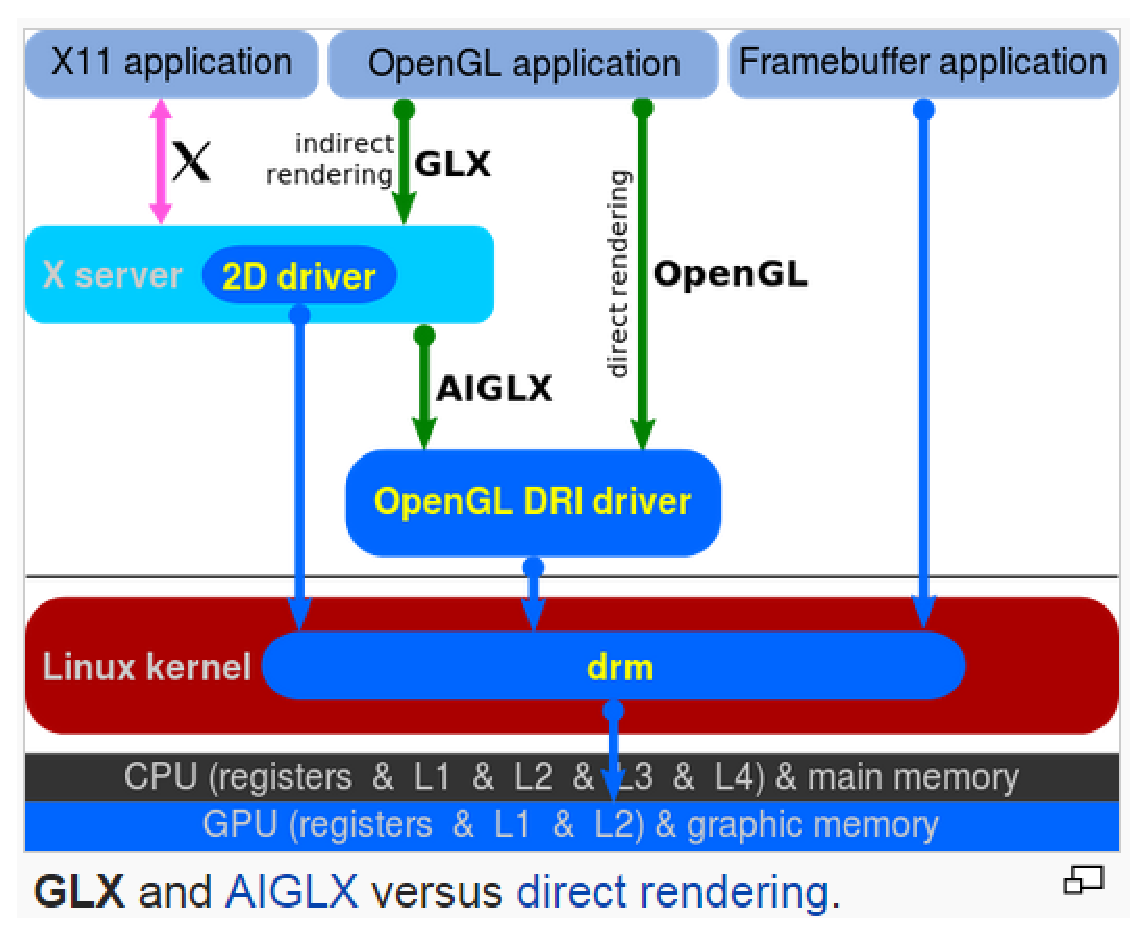
\includegraphics[height=5cm,
    angle=0]{./images/OpenGL_Xserver.eps}}
\caption{{\bf drm} of the kernel control access to the GPU.}
\label{fig:OpenGL_Xserver}
\end{figure}

\subsection{GLX protocol (OpenGL + X11)}
\label{sec:GLX}

{\bf GLX} protocol enables using OpenGL from a window provided by X Windows
System (Sect.\ref{sec:X11}). It provides APIs that connect the OpenGL library
to the X Window System by managing window handles and rendering contexts.
The library is a set of functions and routines that initialize the pixel format,
control rendering, and perform other OpenGL specific tasks.
As of 2011 GLX has reached version 1.4.

The GLX extension was first implemented in XFree86 (Sect.\ref{sec:XFree86}).
\begin{verbatim}
/usr/X11R6/lib/modules/extensions/libglx.a
\end{verbatim}
The part of XServer that renders OpenGL commands for GLX protocol is {\bf
GLcore} - implemented as a software-only version of Mesa, and is used when the
DDX driver does not support DRI. 
\begin{verbatim}
/usr/X11R6/lib/modules/extensions/libGLcore.a
\end{verbatim}
{\bf Utah GLX} is the free early implementation of GLX protocol on Linux-based
O/S, Fig.\ref{fig:XServer_rendering}(2). This was replaced by DRI
implementation.

\subsection{DRI}
\label{sec:DRI}

{\bf DRI} is a framework for allowing direct access to graphics hardware in a
safe and efficient manner.  Without the DRI programs have to perform the
rendering using software.
For example, games or graphics programs can send commands directly to your card
and let it perform fast, hardware-accelerated rendering producing high-quality
visuals. At the same time your CPU is free to do other work. This is known as
direct rendering.

DRI was first made available in XFree86 (Sect.\ref{sec:XFree86}), and is now
part of X11 (Sect.\ref{sec:XServer}).

Initially, the DRI requires a working installation of XFree86 version 4.0.0 or
later, and Linux kernel 2.4.0+. \url{http://dri.sourceforge.net/doc/DRIbeginner.html}
OpenGL-based programs must link with the \verb!libGL! library,
which implements the GLX interface as well as the main OpenGL API entrypoints
(Sect.\ref{sec:GLX}).
\begin{itemize}
  \item When using indirect rendering, libGL creates GLX protocol messages and
  sends them to the X server via a socket. 
  \item When using direct rendering, libGL loads the appropriate 3D DRI driver
  then dispatches OpenGL library calls directly to that driver.
\end{itemize}

The DRI is not a single, isolated piece of software. Instead, the DRI is
composed of a number of distinct modules. 

In 2008 the binding in GLcore to the Mesa software render was rewritten as a DRI
interface module, called \verb!swrast_dri.so!, improving the coupling of Mesa
and the X server. In the same year, a new DRI2 was introduced to replace DRI,
and with it a new model based in the Kernel mode-setting, which uses 
global GEM handles to pass objects (huge securities issues).

DRI3 was proposed in 2012. DRI3 revolves around using POSIX file descriptors for
passing kernel objects between the display server and the application, instead
of passing global GEM handles
\url{http://en.wikipedia.org/wiki/Direct_Rendering_Infrastructure}

To translate these functions in GLX library to Windows: 
\url{https://msdn.microsoft.com/en-us/library/windows/desktop/dd374297(v=vs.85).aspx}

\subsection{AIGLX}
\label{sec:AIGLX}

Accelerated Indirect GLX (AIGLX) brings hardware acceleration to the GLX
(indirect context) applications by loading the Mesa DRI driver inside the X
server, Fig.\ref{fig:XServer_rendering}(4).

\section{OpenGL and Wayland}

Since Linux kernel 3.12, render nodes were introduced,
Fig.\ref{fig:OpenGL_Wayland}.

Wayland (Sect.\ref{sec:Wayland}) implements direct rendering over EGL

\begin{figure}[hbt]
  \centerline{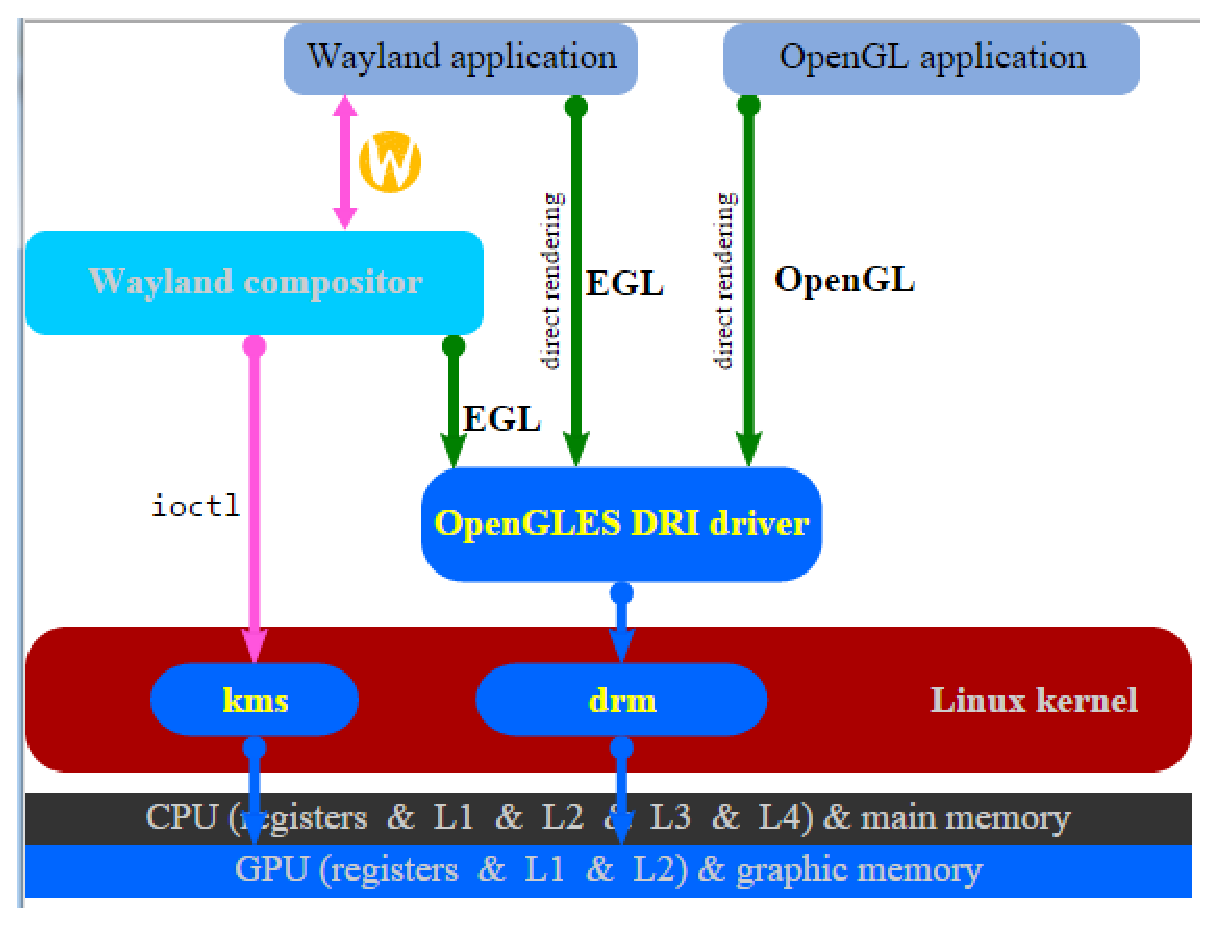
\includegraphics[height=5cm,
    angle=0]{./images/OpenGL_Wayland.eps}}
\caption{OpenGL and Wayland}
\label{fig:OpenGL_Wayland}
\end{figure}



\section{Libraries that use OpenGL}

All OpenGL API-based software/libraries are given in here:
\begin{itemize}
\item \url{http://www.opengl.org/products/platform/C5/P250/}. 
\item  \url{http://www.codemonsters.de/home/content.php?show=freelibraries}

\end{itemize}

All OpenGL functions has \verb!gl!  suffix. Libraries that is built on
top of OpenGL are
\begin{enumerate}
\item \verb!GLU! - Sect.\ref{sec:glu}
 
\item \verb!GLUT! (all function start with \verb!glut! prefix), yet it
  is no longer maintained. Alternative choices are FREEGLUT, SDL,
  OpenML...\footnote{\url{http://www.opengl.org/resources/libraries/windowtoolkits/}}
   
\item \verb!FREEGLUT! : a reimplementation of GLUT

\item \verb!OpenGLUT! : a folk of FREEGLUT

\item \verb!SDL!

\item GUI development: use \verb!GLUI! or \verb!FLTK!

\item Help managing extensions easier: \verb!GLEW! or \verb!GLEE!

\item High-level object-oriented scene graph: \verb!OpenSceneGraph!,
  \verb!OpenSG! ...(commercial product, help creating real-time
  visual simulation application). 
 
\item GLGraphics\footnote{\url{http://glgraphics.sourceforge.net/}}:
  provide a set of classes to simplify the handling of OpenGL texture,
  GLSL shaders and off-screen rendering
\end{enumerate}

GLX (OpenGL GL extensions to the X windows system) integrate
OpenGL with the X Window System. There are different implementation of OpenGL
specification, e.g. GLU (GL Utility), Mesa 3D, GLUT (Chap.{chap:glut}).


\subsection{GLU (for drawing)}
\label{sec:glu}

GLU ({\bf OpenGL Utility Library}) provides a set of higher level drawing
functions implemented on top of OpenGL, i.e.
primitive rendering and mapping between screen- and world-coordinates, etc.

The functions have prefix \verb!glu!. Among these features are
\begin{enumerate}
\item mapping between screen-
  and world-coordinates, 
\item generation of texture mipmaps (MIP maps - a precalculated,
  optimized collections of images that accompany a main texture -
  aimed to improve rendering speed and reduce aliasing artifacts),
\item drawing of quadric surfaces, NURBS (Non-uniform rational
  B-spline), tessellation of polygonal primitives, interpretation of
  OpenGL error codes, 

\item an extended range of transformation routines for setting up
  viewing volumes and simple positioning of the camera, generally in
  more human-friendly terms than the routines presented by OpenGL. 
\end{enumerate}
It also provides additional primitives for use in OpenGL applications,
including spheres, cylinders and disks.

\begin{framed}
  SGI Sample Implementation (SI) include GLU 1.3; while Mesa 3D only
  implements GLU 1.2. So, if you use GLU, it's recommended to install
  SGI SI GLU which is included in the Mesa 3D
  distribution\footnote{\url{http://www.mesa3d.org/glu.html}}.
\end{framed}

\subsection{GLUT (for utilities)}
\label{sec:glut-2}

GLUT ({\bf OpenGL Utility Toolkit}) is a library of utilities for OpenGL.
It contains a set of utilities which focus on window definition, window control
and monitoring of keyboard and mouse input.

Utilities include
\begin{enumerate}
\item functions for window definition, window control, and monitoring
  of keyboard and mouse input.
\item Routines for drawing a number of geometric primitives (both in
  solid and wireframe mode) are also provided, including cubes,
  spheres, and the Utah teapot. GLUT even has some limited support for
  creating pop-up menus.
\end{enumerate}

Any functions of GLUT has the prefix \verb!glut!. GLUT is no-longer
under development, for more information, read Chap.~\ref{chap:glut}. An
alternative choice is freeGLUT (Sect.~\ref{sec:freeglut}).

\subsection{GLEW (loading OpenGL extensions)}
\label{sec:glew}

{\bf OpenGL Extension Wrangler Library} (GLEW) is an opensource multiplatform
library that helps in querying and loading OpenGL Extensions
(Sect.\ref{sec:extensions}).

OpenGL core and extension functionality is exposed in a single header file.
To use GLEW, 
\begin{enumerate}
\item In C/C++: include the file ``GL/glew.h''
\item In Fortran: link to ..., and create an explicit interface to the
  function you want to use
\end{enumerate}

GLEW provides an easy way to get access to the OpenGL extension.  GLEW
can be installed from here:
\url{http://sourceforge.net/projects/glew/}. However, most Linux
distro should have it installed.  

To check for OpenGL extensions being supported, you can use the utility
\verb!glewinfo! (package: glew-utils).

In your code, you can call \verb!glewInit()! and check the error code
\begin{verbatim}
    int err = glewInit();
    // Warning: This does not check if all extensions used
    // in a given implementation are actually supported.
    if (GLEW_OK != err) {
        printf((char*)glewGetErrorString(err));
        exit(ERROR_GLEW);
    }
\end{verbatim}

\begin{enumerate}
\item \verb!glew.h!: OpenGL Extension Wrangler Library that helps
  querying and loading OpenGL extensions. It helps determining which
  extension is supported on your platform

\item \verb!glext.h!: OpenGL Easy Extension Library automatically
  links OpenGL extension and core functions at initialization time
\end{enumerate}

To use in Fortran, you need to link to the library provided in CUDA
SDK
\begin{verbatim}
! 64-bit
-L/usr/local/NVIDIA_GPU_COMPUTING_3.1/C/common/lib/linux/ -lGLEW_x86_64

! 32-bit
-L/usr/local/NVIDIA_GPU_COMPUTING_3.1/C/common/lib/linux/ -lGLEW
\end{verbatim}
NOTE: In CUDA 5.0, the library is renamed, using the same name libGLEW.a for
both 32-bit and 64-bit; yet the file locations are different.
\begin{verbatim}
/usr/local/cuda5.0/samples/common/lib/linux/i686/libGLEW.a
/usr/local/cuda5.0/samples/common/lib/linux/x86_64/libGLEW.a
\end{verbatim}

After linking to the library, then you just define an explicit interface to the
function that you want to use, e.g.
\begin{verbatim}
  INTERFACE
    FUNCTION glewInit() BIND(c, name="glewInit") RESULT(res)
      USE iso_c_binding
      INTEGER(C_INT) :: res
    END FUNCTION glewInit
  END INTERFACE
\end{verbatim}

\url{http://glew.sourceforge.net/install.html}

\section{OpenGL-ES}
\label{sec:OpenGL-ES}

OpenGL-ES (OpenGL for Embedded Systems) is a subset of OpenGL designed for use
on embedded systems like smartphones, tablets, game consoles, etc.

\subsection{WebGL}
\label{sec:WebGL}

Take in mind that they might have the same functions, though WebGL isn't OpenGL
or OpenGL-ES. WebGL is only based on OpenGL-ES.
{\bf WebGL} - based on OpenGL ES 2.0 
provides APIs in JavaScript for 3D rendering on the webbrowser.




\section{Rendering and Coordinate systems}
\label{sec:coordinate-systems}

\begin{figure}[hbt]
  \centerline{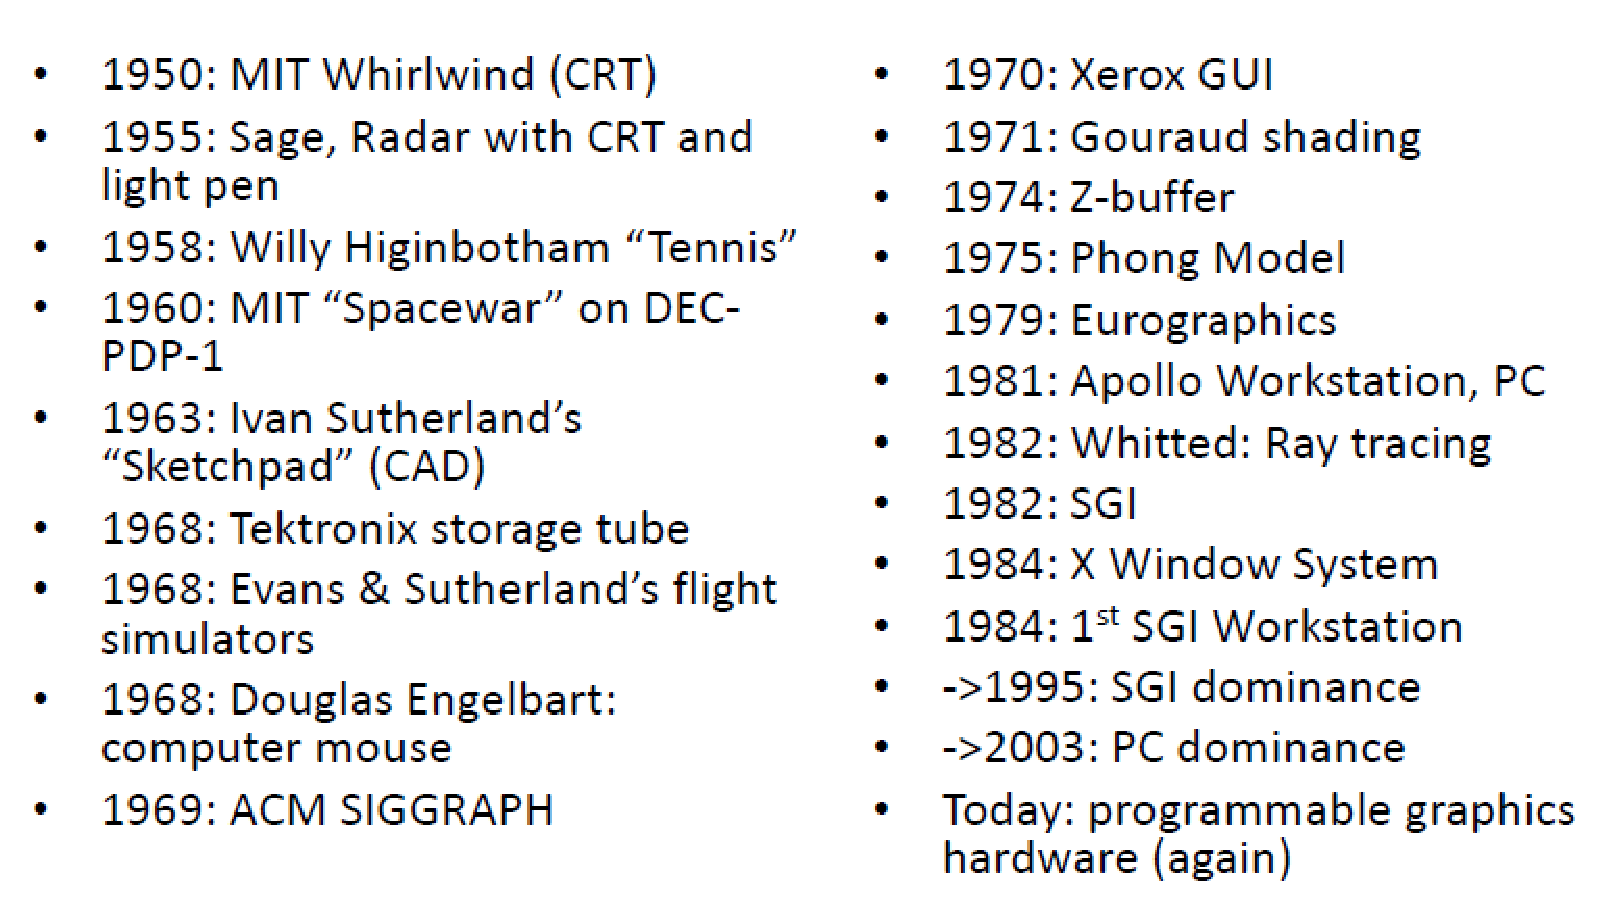
\includegraphics[height=5cm,
    angle=0]{./images/history.eps}}
\caption{History of computer graphics }
\label{fig:history}
\end{figure}

The history of computer graphics is given Fig.\ref{fig:history}.
An object in 3D space is represented via thousands of geometric
primitives (lines, triangles, points). In order to generate a view,
the programmer need to define a ``virtual camera'' and a viewing
angle.  Rasterization takes every vertex, primitives and maps them to
the pixels on the screen.

Before we can describe an object in 3D, we need a coordinate system,
i.e. a frame of reference to measure and locate the object. We have a
number of coordinate system
\begin{enumerate}
\item real world coordinate system (or drawing coordinate): this is
  the system that we define to capture the scene.  The origin is aka
  the location of the ``virtual camera'' and a viewing angle.

\item window coordinate system: this is the system that we define the
  location of objects on the window, the unit is measured in pixels.

\item screen coordinate system: this is the system that we define that
  location of windows on the screen, the unit is measured in pixels,
  e.g. 640x480 in pixels.
\end{enumerate}
These coordinate systems can be based on 
\begin{itemize}
\item 2D Cartesian coordinate, i.e. origin is (x=0,y=0) and the two
  axises are orthogonal. So, how we choose the origin in such system,
  using 2D Cartesian coordinate, will affect the value of the
  coordinate of the objects, Fig.~\ref{fig:clipping}. 
\begin{figure}[hbt]
  \centerline{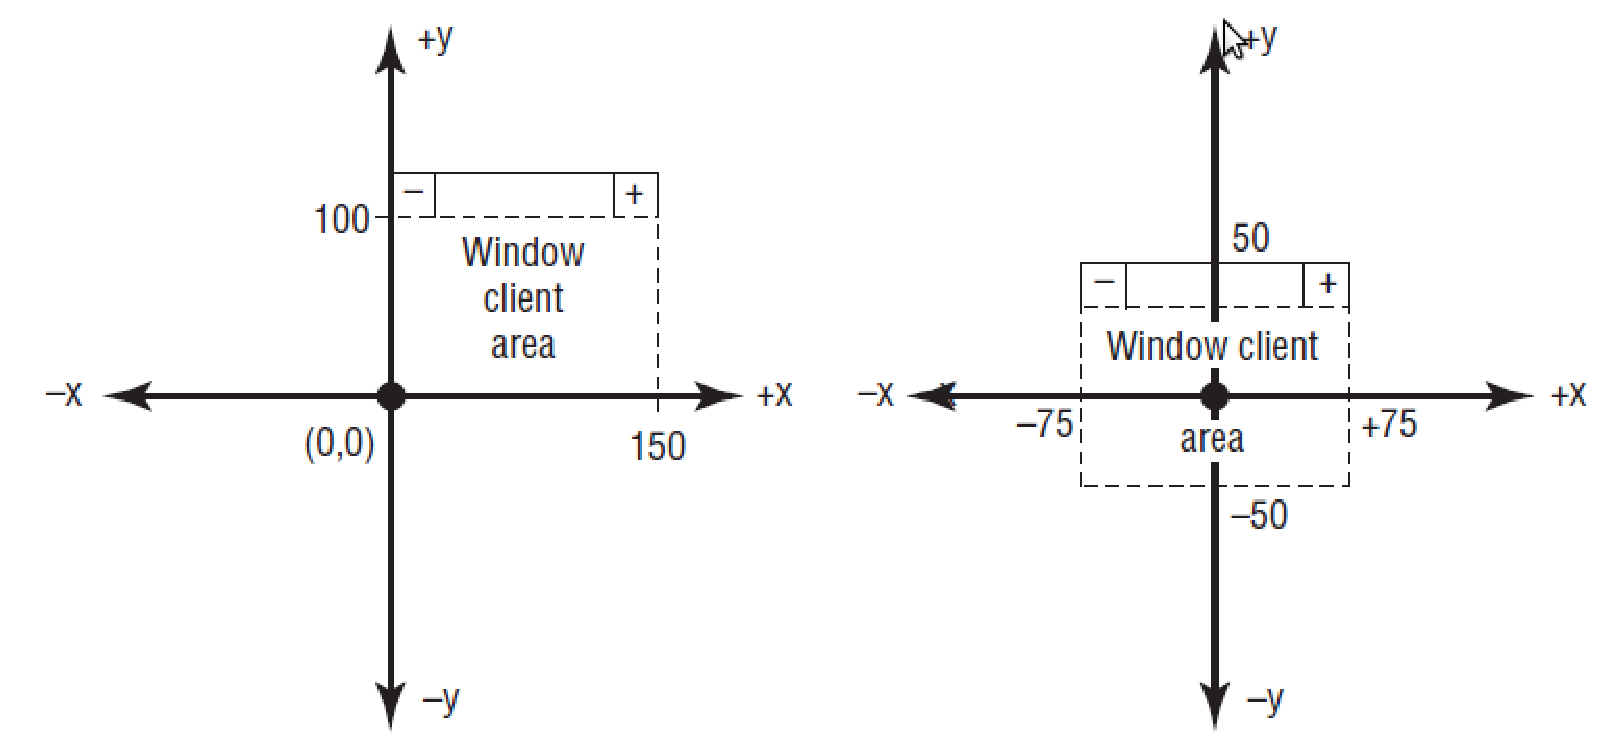
\includegraphics[height=5cm,
    angle=0]{./images/clipping.eps}}
\caption{Two clipping regions}
\label{fig:clipping}
\end{figure}

Using OpenGL we can also turn the coordinate system upside down or
flip it right to left.
\textcolor{red}{In fact, the default mapping for Windows windows is
  for positive $y$ to move down from the top to bottom of the
  window} which is not convenient for drawing graphics. 

You cannot capture the whole real-world, but just a scene of it. This
is known as {\bf clipping}. 

{\bf Viewport}: Rarely, the clipping area of the scene fit the screen
size. So, you need to map from logical Cartesian coordinates to the
area on the physical screen pixel coordinates. This setting is known
as {\bf Viewport}. The viewport is the region within the window on the
physical screen. Normally, the viewport is the entire window, but this
isn't necessary true, Fig.~\ref{fig:viewport}.

\begin{figure}[hbt]
  \centerline{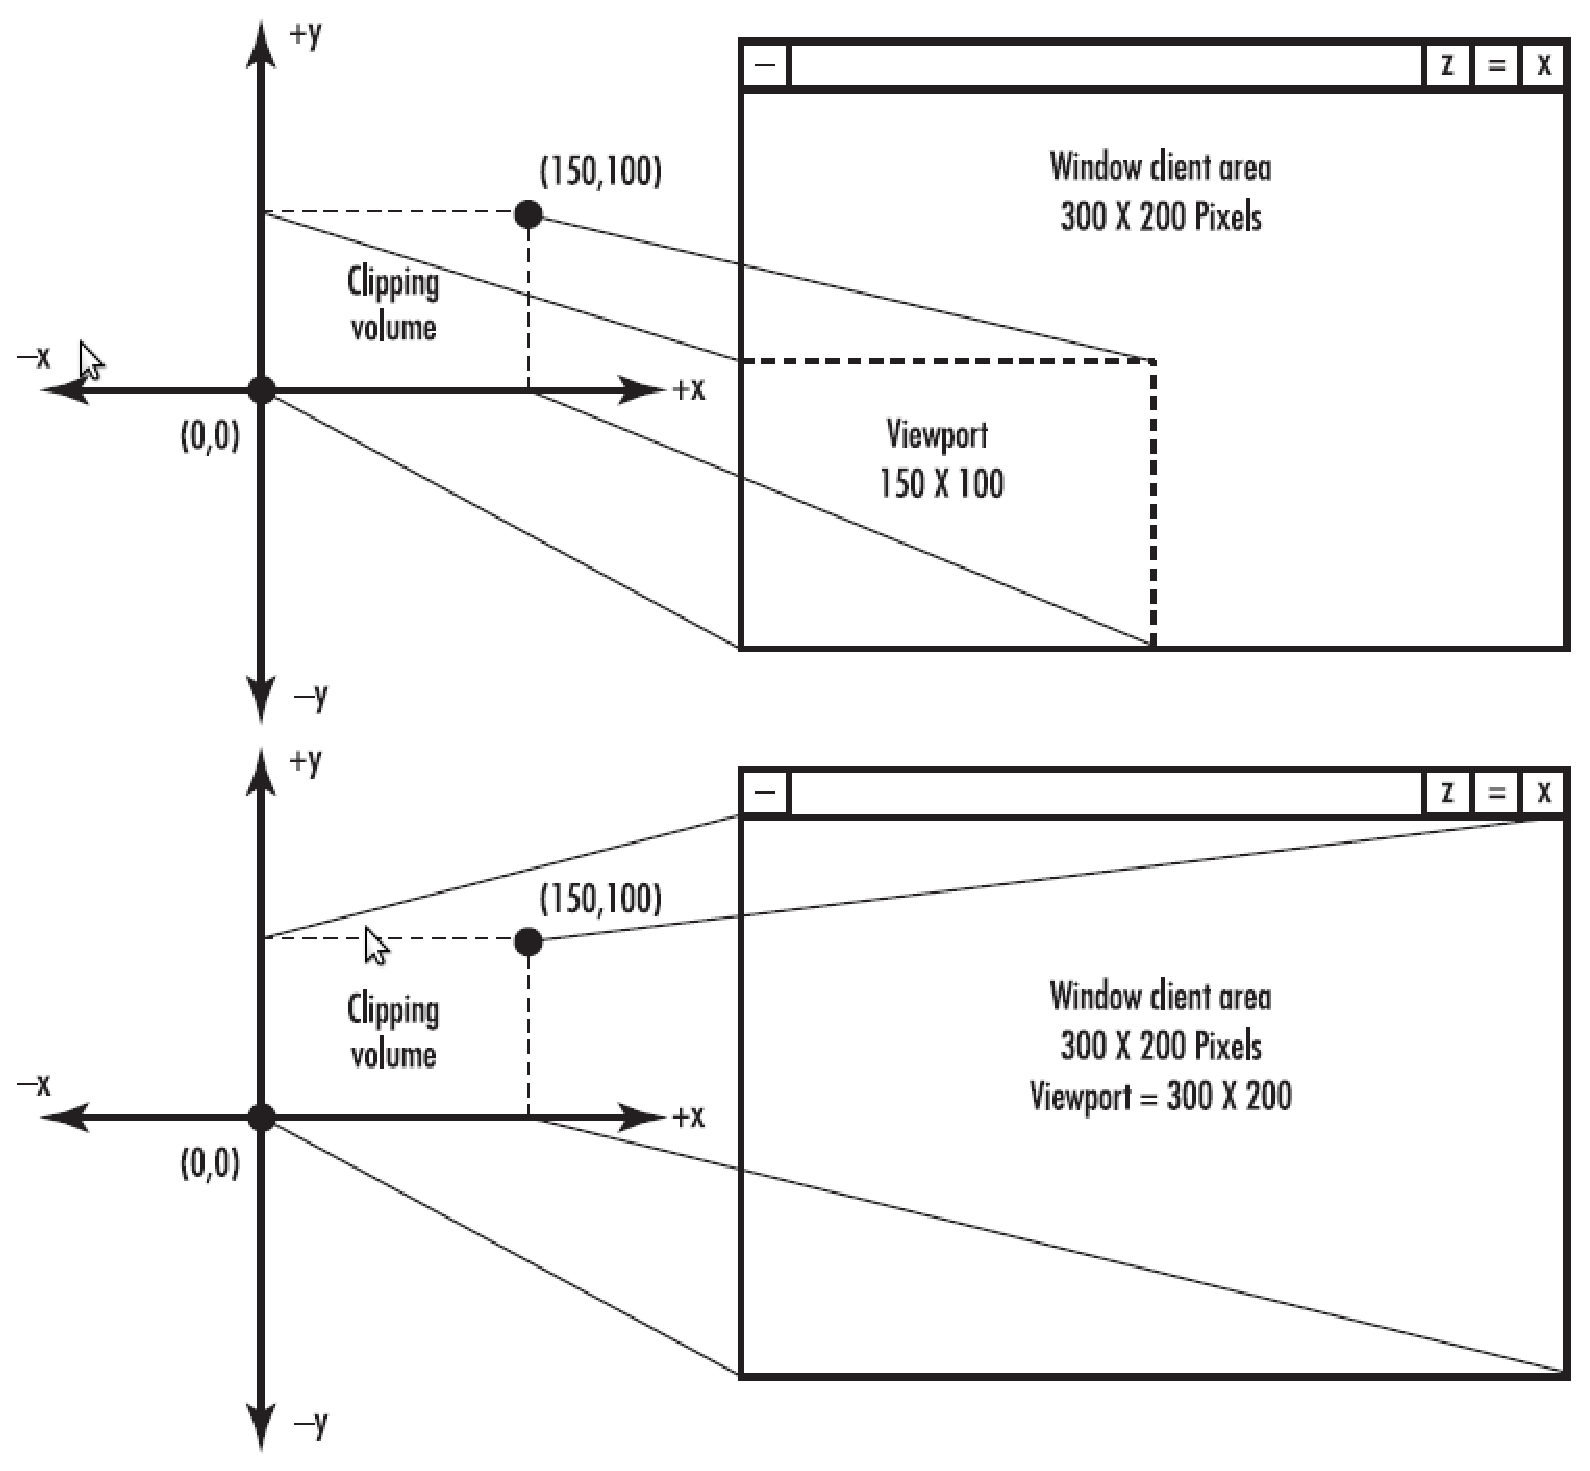
\includegraphics[height=5cm,
    angle=0]{./images/viewport.eps}}
\caption{Two different viewports}
\label{fig:viewport}
\end{figure}

\item 3D Cartesian coordinate, i.e. origin is (x=0, y=0, z=0) and we
  have three axises, orthogonal in pair. Now, instead of a clipping
  area, we have the concept of {\bf clipping volume} (or viewing
  volume, anything outside of this is not drawn).

  So, not only we need to define {\bf viewport}, but also we need to
  define a {\bf projection} which tells how to map 3D coordinates in
  the viewing volume onto a position on the 2D surface. There are two
  ways of projections
  \begin{enumerate}
  \item {\bf orthogonal projection} (or parallel projection),
    Fig.~\ref{fig:orthogonal_projection}: the viewing volume is a
    square or rectangle viewing volume. This type of projection sis
    most often used in architectural design, computer-aided design
    (CAD), or 2D graphs.
\begin{figure}[hbt]
  \centerline{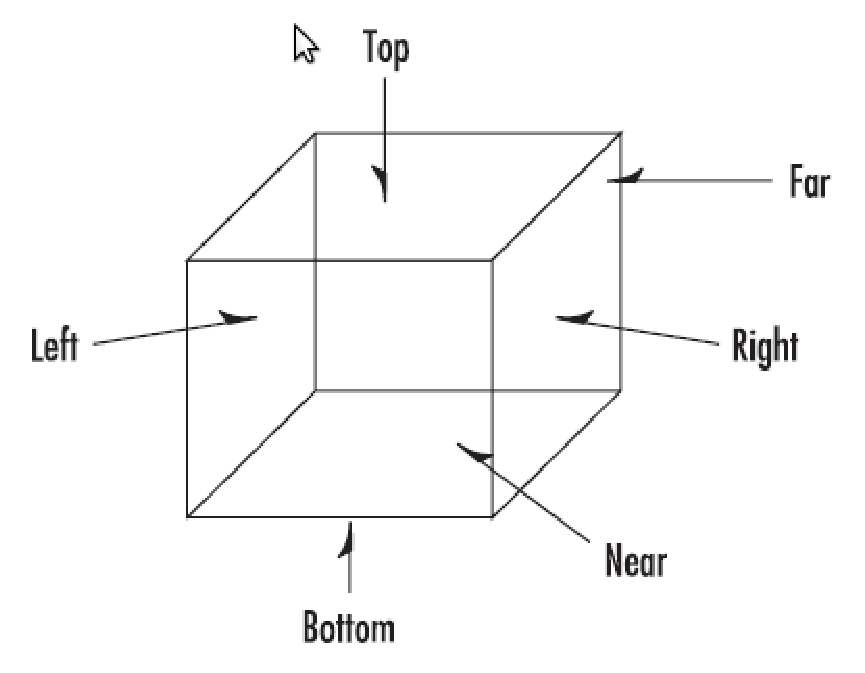
\includegraphics[height=5cm,
    angle=0]{./images/orthogonal_projection.eps}}
  \caption{We need to specify the far, near, left, right, top, and
    bottom clipping planes}
\label{fig:orthogonal_projection}
\end{figure}

\item {\bf perspective projection}: this give you a more realistic
  view, as the size of the planes are different. The clipping volume
  looks like a pyramid with the top shave-off (the shape known as
  {\bf frustum}). Objects near the front of the viewing volume appear
  close to their original size, and those near the back of the viewing
  volume shrink as they are projected on the 2D display,
  Fig.~\ref{fig:perspective_projection}.

\begin{figure}[hbt]
  \centerline{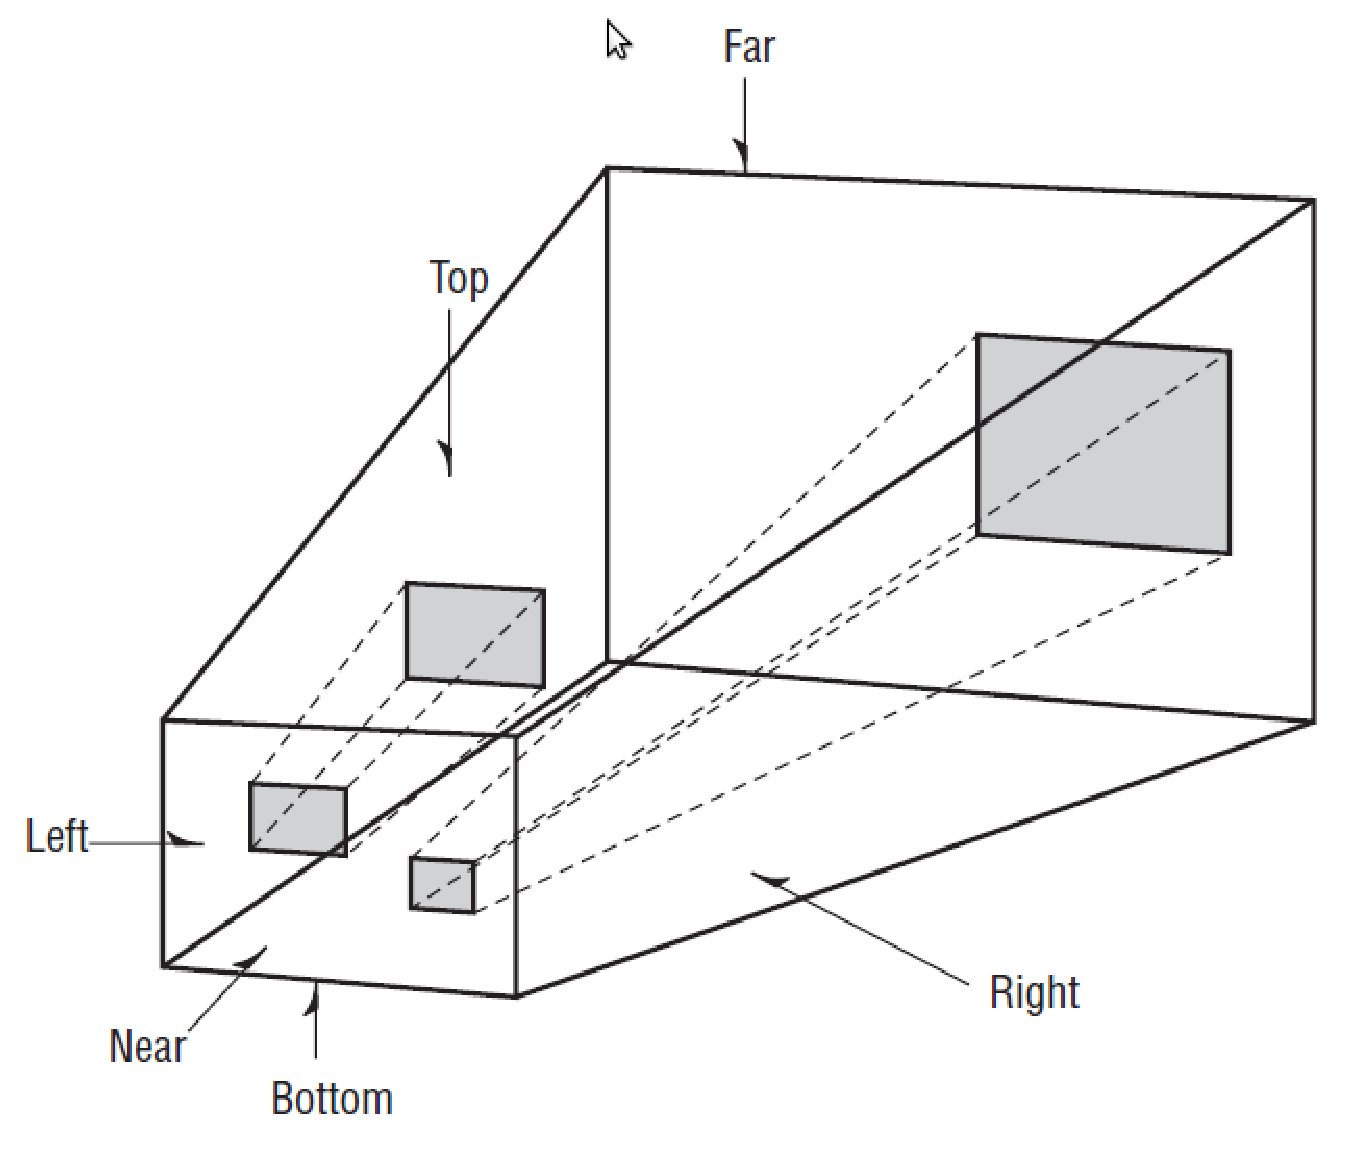
\includegraphics[height=5cm,
    angle=0]{./images/perspective_projection.eps}}
 \caption{Perspective projection}
\label{fig:perspective_projection}
\end{figure}

  \end{enumerate}


\end{itemize}

For more detail, read Sect.~\ref{sec:rendering}. 

% 
% OpenGL is widely used in scientific visualization, CAD, virtual
% reality, video games... Its rival is Direct3D from Microsoft which is
% being used mostly in video games.



\section{GLSL}
\label{sec:GLSL}

GL Shading Language (GLSL).

\section{Shaders}
\label{sec:shaders}

In sect.~\ref{sec:clientserver}, we have learnt that shaders are the
program that run on GPU (not CPU) and do the drawing. The two main types are
vertex shader and pixel shader. The stream of a 3D model flows from application,
to vertex shader, to pixel shader, and finally to the frame buffer
\footnote{\url{http://www.neatware.com/lbstudio/web/hlsl.html}}.
A simple vertex shader program, which receive a data structure (a2v)
transferred from an application to it, the output (v2p) will be given to the
pixel shader:
\begin{verbatim}
  void main(in a2v IN, out v2p OUT, uniform float4x4 ModelViewMatrix) 
  {
    OUT.Position = mul(IN.Position, ModelViewMatrix); 
  }
   
  struct a2v { 
    float4 Position : POSITION; 
  };


  struct v2p {
    float4 Position : POSITION;
  };
    
\end{verbatim}
NOTE: \verb!uniform! modifier indicates that the value of the matrix is a
constant assigned by external program. While IN.Position is the left parameter
of mul, it is considered as a row vector. Otherwise it is considered as a column
vector.  

\begin{framed}
You can think HLSL as a C language for GPU programming except there are no
pointer, union, bitwise operations, and function variables. There are no goto,
switch, recursive function in HLSL as well. However HLSL adds vector data type,
build-in constructor, swizzling and masking operators. HLSL standard library
includes mathematical functions and texture processing functions. The function
overloading has been used to unify the operations of different vectors.  
\end{framed}

The pixel shader does other jobs: adding shading information to the pixel
\begin{verbatim}
  struct v2p {
    float4 Position  : POSITION;
    float2 Texcoord0 : TEXCOORD0;
    float2 Texcoord1 : TEXCOORD1;
    float4 Color     : COLOR0;
  };

  void main( in v2p IN, out p2f OUT ) 
  {  
\end{verbatim}
The output p2f will be given to the frame buffer.



There are some predefined types of shaders. So, we need to load the shader we
want.


\subsection{Identity shader}
\label{sec:identity-shader}

The identity shader simply draws geometry using the default Cartesian
coordinate system (-1.0 to 1.0 on all axes).

A single color is applied to all fragments, and the geometry is solid
and unshaded. The only attribute used is
\verb!GLT_ATTRIBUTE_VERTEX!. The vColor parameter contains the desired
color (RGBA).
\begin{verbatim}
GLShaderManager::UseStockShader(GLT_SHADER_IDENTITY, GLfloat vColor[4]);
\end{verbatim}

\subsection{Flat shader}
\label{sec:flat-shader}

This is more complicated than Identity shader, as it provides a 4x4
matrix \verb!mvp! that can be used to do geometry transformation. This
matrix is often called the modelview projection matrix.

Like identify shader, it use only one attribute
\verb!GLT_ATTRIBUTE_VERTEX!.
\begin{verbatim}
GLShaderManager::UseStockShader(GLT_SHADER_FLAT, 
                       GLfloat mvp[16], GLfloat
                       vColor[4]);
\end{verbatim}


\subsection{Shaded shader (smooth shading)}
\label{sec:shaded-shader}

If this shader is used, colors are interpolated smoothly between the
vertices. You need to enable this shader if you want smooth shading
effect.  Both the \verb!GLT_ATTRIBUTE_VERTEX! and the
\verb!GLT_ATTRIBUTE_COLOR! are used by the shader.

\begin{verbatim}
GLShaderManager::UseStockShader(GLT_SHADER_SHADED, GLfloat mvp[16]);
\end{verbatim}

\subsection{Default Light shader}
\label{sec:default-light-shader}

If you want to have the effect of shade and lit, this shader create
the illusion of a single diffuse light source located at the eye
position (if you want to put the light source at a different position,
use Point Light shader). 

\begin{verbatim}
GLShaderManager::UseStockShader(GLT_SHADER_DEFAULT_LIGHT, 
                 GLfloat mvMatrix[16],
                 GLfloat pMatrix[16], GLfloat vColor[4]);
\end{verbatim}

Most lighting shaders require the normal matrix as a uniform. This
shader derives the normal matrix from the modelview matrix - convenient,
but not terribly efficient. So, not a recommend for
performance-sensitive applications.


Required attributes are \verb!GLT_ATTRIBUTE_VERTEX! and
\verb!GLT_ATTRIBUTE_NORMAL!.

\subsection{Point Light shader}
\label{sec:point-light-shader}

\begin{verbatim}
GLShaderManager::UseStockShader(GLT_SHADER_POINT_LIGHT_DIFF, 
                     GLfloat mvMatrix[16],
                     GLfloat pMatrix[16], 
                     GLfloat vLightPos[3], //light source
                     GLfloat vColor[4]);
\end{verbatim}

\subsection{Texture Replace shader}
\label{sec:text-repl-shad}

\begin{verbatim}
GLShaderManager::UseStockShader(GLT_SHADER_TEXTURE_REPLACE,
GLfloat mvpMatrix[16], GLint nTextureUnit);
\end{verbatim}

\subsection{Texture Modulate shader}
\label{sec:text-modul-shad}

\begin{verbatim}
GLShaderManager::UseStockShader(GLT_SHADER_TEXTURE_MODULATE, 
             GLfloat mvpMatrix[16],
             GLfloat vColor, GLint nTextureUnit);
\end{verbatim}

\subsection{Textured Point Light shader}
\label{sec:textured-point-light}

\begin{verbatim}
GLShaderManager::UseStockShader(GLT_SHADER_TEXTURE_POINT_LIGHT_DIFF,
    GLfloat mvMatrix, GLfloat pMatrix[16], GLfloat vLightPos[3],
    GLfloat vBaseColor[4], GLint nTextureUnit);
\end{verbatim}

Above are pre-defined shaders. Users nowadays can write their own
shaders. 

\section{2D Array = Texture = Pixmap}
\label{sec:arrays-=-textures}

Native memory layout in CPU is in 1D. Any higher dimensional array
will eventually mapped to 1D by the compiler. 
However, in GPU, native data layout is 2D. 1D and 3D arrays are also
supported in GPU, however they may impose a performance penalty.

\begin{framed}
  A texture is an image (2D) that can be applied to a triangle in your
  scene - the process known as {\bf texture mapping}. So the solid
  area is filled with {\bf texels} - the texture-based equivalent of
  pixel.

  Original electronic computer display data in monochrome (one color)
  with each pixel can receive on or off value (0 or 1). So an image is
  represented as a {\bf bitmap} - a series of 1s and 0s (in 1D). 

  In grayscale images, each pixel can receive one of 256
  values. Windows has the .BMP file extension that hold this picture
  file format.The image with each pixel represented by more than one
  bit is called {\bf pixmap} (pixel rectangle).
\end{framed}

\subsection{Front/Back and other buffers}
\label{sec:frontb-other-buff}

OpenGL stores and manipulates pixel data in a framebuffer. The
framebuffer is not a real buffers as it doesn't contain data. It
indeed serves as a container that hold other buffers, e.g. color
buffer, depth buffer, accumulation buffer and stencil buffers. It is
these buffers that hold true data. 

The color buffer contains a set of logical buffers (front-left,
front-right, back-left, back-right and some number of auxiliary
buffers). An implementation OpenGL many not supply all of these
buffers. However, most implementations support {\bf double buffering
  of images}. This is a technique in which an application draw pixels
to an off-screen buffer, and then when that image is ready for
display, the application copies the content of the off-screen buffer
to an on-screen buffer. Double buffering enables smooth image changes,
which is especially important for animated images. GLUT/FreeGLUT
help make it easier for user by providing
\begin{enumerate}
\item \verb!GLUT_DOUBLE! option
\item \verb!glutSwapBuffers()! function (call when the off-screen
  buffer is ready for display)
\end{enumerate}

In Windows, we set \verb!PFD_DOUBLEBUFFER! flag in the
PIXELFORMATDESCRIPTOR data structure. 

When color are written to a framebuffer, they are written to the color
buffer specified by \verb!glDrawBuffer()!. Even though you can write
to a single color buffer at a time, you can select more than one color
buffer (with written data) for drawing. This help creating {\bf
  blending effect}. .

\subsection{Pixel packing}
\label{sec:pixel-packing}

Image data is rarely packed tightly into memory. The reason is that
each row of an image should start at some particular byte-aligned
address for optimal performance. OpenGL use 4-byte alignment. So, it's
best to use RGBA for a pixel. 

.BMP use 4byte-aligned format; yet .TGA use 1byte-aligned format. You
can change how tightly packed pixel data using
\begin{verbatim}
// tell how OpenGL unpack data from data buffers
glPixelStorei(GL_UNPACK_ALIGNMENT, 1);

// tell how OpenGL pack data being read from pixel buffers
// and place them into a user-specified memory buffer
glPixelStorei(GL_PACK_ALIGNMENT, 1);


// syntax:
void glPixelStorei(GLenum pname, GLint param);
void glPixelStoref(GLenum pname, GLfloat param);
\end{verbatim}

\subsection{Pixmap}
\label{sec:pixmap}

We cannot draw a pixmap directly into the color buffer but you can
read the content of the color buffer directly as a pixmap. This data
is copied back to the client side memory during which your application
is blocked until the transfer has completed (for GPU-to-GPU memory
copy, read Sect.~\ref{sec:buffer-objects} and
Sect.~\ref{sec:cuda-app.-with}). In addition, if you specify a pixel
layout different from the native arrangement of your graphics
hardware, there will be an additional performance penalty as the data
is reformatted.
\begin{verbatim}
void glReadPixels(GLint x, GLint y, GLSizei width, GLSizei height,
GLenum format, GLenum type, const void *pixels);
\end{verbatim}
with the x and y in window coordinates of the lower-left corner of the
rectangle to read followed by width and height of the rectangle in
pixels. If the color buffer stores data differently than what you have
requested, OpenGL takes care of the necessary conversions.  This
capability can be very useful. The pointer to the image data, *pixels,
must be valid and must contain enough storage to contain the image
data after conversion, or you will likely get a nasty memory exception
at runtime. Also be aware that if you specify window coordinates that
are out of bounds, you will get data only for the pixels within the
actual OpenGL frame buffer. The fourth argument specify the color
layout, which can be any thing in Table.~\ref{tab:OpenGL_color}. The
fifth argument tell the type for each color component,
Table~\ref{tab:pixel_data_type}. 


For our glReadPixels function, by default, the read operation is
performed on the back buffer for double-buffered rendering contexts,
and the front buffer for single-buffered rendering contexts. You can
change the source of these pixel operations by using this function:
\begin{verbatim}
void glReadBuffer(GLenum mode);
\end{verbatim}
The mode parameter can be any one of 
\begin{verbatim}
GL_FRONT, GL_BACK, GL_LEFT, GL_RIGHT,
GL_FRONT_LEFT, GL_FRONT_RIGHT, GL_BACK_LEFT, 
GL_BACK_RIGHT, or even GL_NONE.
\end{verbatim}


\subsection{Loading texture (1D, 2D, 3D)}
\label{sec:loading-texture}

The first step before you can write a texture to a solid area is to
load the texture (image data) (e.g. from a disk file) into the memory.
\begin{verbatim}
void glTexImage1D(GLenum target, GLint level, GLint internalformat,
       GLsizei width, GLint border,
       GLenum format, GLenum type, void *data);

void glTexImage2D(GLenum target, GLint level, GLint internalformat,
       GLsizei width, GLsizei height, GLint border,
       GLenum format, GLenum type, void *data);

void glTexImage3D(GLenum target, GLint level, GLint internalformat,
       GLsizei width, GLsizei height, GLsizei depth, GLint border,
       GLenum format, GLenum type, void *data);
\end{verbatim}
OpenGL supports one-, two-, and threedimensional texture maps and uses
the corresponding function to load that texture and make it
current. This data copy can be quite expensive.

The target argument for these functions should be
\verb!GL_TEXTURE_1D!, \verb!GL_TEXTURE_2D!, or \verb!GL_TEXTURE_3D!,
respectively. You may also specify proxy textures by specifying
\begin{verbatim}
GL_PROXY_TEXTURE_1D, GL_PROXY_TEXTURE_2D, or GL_PROXY_TEXTURE_3D 
\end{verbatim}
using the function \verb!glGetTexParameter()! to retrieve the results
of the proxy query (read Sect.~\ref{sec:proxy-texture}). 

The \verb!level! tells the mipmap level being loaded (for non-mipmap,
set it to 0) (read Sect.~\ref{sec:mipmap-generation}).

The \verb!internalformat! parameter of the texture data. This
information tells OpenGL how many color components you want stored per
texel and possibly the storage size of the components and/or whether
you want the texture compressed,
Table~\ref{tab:texture_internal_format}.

\begin{framed}
  The width, height, and depth parameters (where appropriate) specify
  the dimensions of the texture being loaded. It is important to note
  that prior to OpenGL 2.0, these dimensions must be integer powers of
  2 (1, 2, 4, 8, 16, 32, 64, and so on). 

  There is no requirement that texture maps be square (all dimensions
  equal), but a texture loaded with non-power of 2 dimensions on older
  OpenGL implementations will cause texturing to be implicitly
  disabled. Even though OpenGL 2.0 (and later) allows non-power of 2
  textures, this is no guarantee that they will necessarily be fast on
  the underlying hardware. Many performance-minded developers still
  avoid non-power of two textures for this reason.
\end{framed}
.

\begin{table}[hbt]
\begin{center}
\caption{Texture internal format}
\begin{tabular}{cc} 
\hline
\verb!GL_ALPHA!& Store the texels as alpha values\\
\verb!GL_LUMINANCE!& Store the texels as luminance values\\
\verb!GL_LUMINANCE_ALPHA! & Store the texels with both luminance and alpha values\\
\verb!GL_RGB!& Store the texels as red, green, and blue components\\
\verb!GL_RGBA! & Store the texels as red, green, blue, and alpha components\\
\hline\hline
\end{tabular}
\end{center}
\label{tab:texture_internal_format}
\end{table}

The border parameter allows you to specify a border width for texture
maps. Texture borders allow you to extend the width, height, or depth
of a texture map by an extra set of texels along the borders. Texture
borders play an important role in the discussion of texture filtering
to come. For the time being, always set this value to 0 (zero).


The last three parameters ``format, type, and data" are identical to the
corresponding arguments when you used glReadPixels in the previous
section. 

\subsection{Proxy texture}
\label{sec:proxy-texture}



\subsection{Cubemap texture}
\label{sec:cubemap-texture}


Arrays in GPU is called {\bf textures} or {\bf texture samplers}.
Texture dimensions are limited on GPUs, the maximum value in each
dimension can be queried with a bit of code like this once a valid
OpenGL context is available (that is, once GLUT is initialized). On
today's graphics card, the maximum range is 2048 or 4096 per
dimension.

\begin{verbatim}
int maxtexsize;

glGetIntegerv(GL_MAX_TEXTURE_SIZE,&maxtexsize);

printf("GL_MAX_TEXTURE_SIZE, %d\n",maxtexsize);   
\end{verbatim}


In CPU, we usually talk about {\bf array indices}. In GPU, however, we
use {\bf texture coordinates} to get access to the value stored in the
textures with the notation is S, T, and R. Texture coordinates need to
address texel centers.

\begin{framed}
  Traditionally, GPUs work on four-tupels of data simultaneously:
  There are four color channels called red, green, blue and alpha
  (RGBA). We will explain later on how we can exploit this to speed up
  our implementation on certain hardware.
\end{framed}


\textcolor{red}{Working with texture is easy once we know texture
  target, texture format and internal format} we want to use:

\begin{enumerate}
\item (named texture) To create a named texture
\begin{verbatim}
GLuint texture;

// allocate a texture name
glGenTextures( 1, &texture );
\end{verbatim}
  use a value higher than 1 if you want to create an array of
  continuous texture names.  The named textures are unsigned integers,
  with the value zero is reserved to represent the default texture for
  each texture target.

\item (texture target) This texture name can be used to bind to any texture target
  using \verb!glBindTexture! function. 
\begin{verbatim}
void glBindTexture(GLenum  target, 
                   GLuint  texture);
\end{verbatim}
  When a texture is bound to a target, the previous binding for that
  target is automatically broken. 
  
  In OpenGL, there are two common forms of texture targets: 1D
  (\verb!GL_TEXTURES_1D!) and 2D (\verb!GL_TEXTURE_2D!) with the
  latter one is more common.  When a named texture bind to
  \verb!GL_TEXTURE_1D!, it becomes a 1D texture; if it bind to
  \verb!GL_TEXTURE_2D!, it becomes a 2D textures...

  \textcolor{red}{The limitation for current OpenGL textures is that
    they requires power-of-two sized dimensions (POTS)},
  e.g. 16, 32, 64... So, resampling is required to convert data to the
  correct dimensions. For non-power-of-two sized textures, read
  Sect.~\ref{sec:nopts-texture}.
\begin{verbatim}
// select our current texture
glBindTexture( GL_TEXTURE_2D, texture );
\end{verbatim}

\item Optional:
  \begin{enumerate}
  \item \verb!glGetBoolean! with \verb!GL_TEXTURE_1D! /
    \verb!GL_TEXTURE_2D! / etc to check whether texture is enabled for
    that dimension. 
  \item \verb!glGetInteger()! to query which texture name is currently
    bound to a particular dimension(beware this used to be an
    extension, so I'm not sure it will be available by default under
    Windows).
  \end{enumerate}

\item Set some texture environment variables
\begin{verbatim}
// select modulate to mix texture with color for shading
glTexEnvf( GL_TEXTURE_ENV, GL_TEXTURE_ENV_MODE, GL_MODULATE );
\end{verbatim}
  \verb!GL_MODULATE! simply takes the color and alpha data from the
  texture and multiplies it with the color data from glColor and/or
  the lighting system.


\item Set some texture parameters which allows us to use wonderful
  effects like bilinear and trilinear texture filtering, and
  mipmapping. 
\begin{verbatim}
// when texture area is small, bilinear filter the closest mipmap
glTexParameterf( GL_TEXTURE_2D, GL_TEXTURE_MIN_FILTER,
                 GL_LINEAR_MIPMAP_NEAREST );
// when texture area is large, bilinear filter the original
glTexParameterf( GL_TEXTURE_2D, GL_TEXTURE_MAG_FILTER, GL_LINEAR );

// the texture wraps over at the edges (repeat)
glTexParameterf( GL_TEXTURE_2D, GL_TEXTURE_WRAP_S, GL_REPEAT );
glTexParameterf( GL_TEXTURE_2D, GL_TEXTURE_WRAP_T, GL_REPEAT );
\end{verbatim}
  We also can setup whether the texture wraps over at the edges or is
  clamped at the ends. We'll stick to repeating because that is the
  most common use. Just read the comments for details on what each
  does.
  \begin{itemize}
  \item For clamped textures, S \& T are in the range of 0 to 1.
  \item For repeated textures, the range is 0 to 1 for every repeat of
    the texture, as is 1 to 2, 2 to 3, and even -1 to 0. Just feed the
    coordinates much like a glColor command, only use the glTexCoord.

  \end{itemize}
  \begin{framed}
    Just remember, any color you fed to glColor is multiplied by the
    texture data, so if your texture is dark or an unusual color,
    check to see what color you are setting to.
  \end{framed}

\item Load the texture data
\begin{verbatim}
/* Suppose the data is RAW */
BYTE * data;
// texture data
width = 256;
height = 256;

data = malloc( width * height * 3 );
// load data into data (in some way)
// or compute the first data
// here, suppose data is from file
    // open texture data
    file = fopen( filename, "rb" );
    if ( file == NULL ) return 0;
    // read texture data
    fread( data, width * height * 3, 1, file );
    fclose( file );
\end{verbatim}
  You could load from PCX, BMP, GIF, JPG, or any other file
  format. You just have to load the image data for OpenGL, and let it
  do the rest. 

\item (Use if mipmap is enable) we create a mipmap. There a function
  to do that, all we need todo is feed it some information on the
  image and the actual image data and it does all the work for us.
\begin{verbatim}
/* Now we can build the texture mipmap */
gluBuild2DMipmaps( GL_TEXTURE_2D, 3, width, height,
                   GL_RGB, GL_UNSIGNED_BYTE, data );
/* free buffer (if we don't need it)
   the mipmap (image data) has been copied to the OpenGL system
*/
free( data );
\end{verbatim}

\item Enable texture mapping
\begin{verbatim}
glEnable( GL_TEXTURE_2D );
\end{verbatim}

\item (internal format) GPUs allow for the simultaneous processing of
  scalars, tupels, tripels or four-tupels of data. In this tutorial,
  we focus on scalars and four-tupels exemplarily. The easier case is
  to allocate a texture that stores a single floating point value per
  texel, i.e. \verb!GL_LUMINANCE!.

\item Now, we specify the 2D texture image
\begin{verbatim}
glTexImage2D(texture_target, 0, internal_format,
             texSize, texSize, 0, texture_format, GL_FLOAT, 0);
\end{verbatim}
The second parameter set to 0 means we don't need to use mipmaps
levels for this texture (i.e. do not create miniature copies). 

The sixth parameter set to 0 means we don't need border (turn off border)

\item Callback\footnote{\url{http://www.nullterminator.net/gltexture.html}}
\begin{verbatim}
glBegin( GL_QUADS );
glTexCoord2d(0.0,0.0); glVertex2d(0.0,0.0);
glTexCoord2d(1.0,0.0); glVertex2d(1.0,0.0);
glTexCoord2d(1.0,1.0); glVertex2d(1.0,1.0);
glTexCoord2d(0.0,1.0); glVertex2d(0.0,1.0);
glEnd();
\end{verbatim}


\item Free the texture
\begin{verbatim}
glDeleteTextures( 1, &texture );
\end{verbatim}
\end{enumerate}

\begin{verbatim}
// create a new texture name
GLuint texID;
glGenTextures (1, &texID);

// bind the texture name to a texture target
// replace texture_texture with appropriate value
glBindTexture(texture_target,texID);

// turn off filtering and set proper wrap mode
// (obligatory for float textures atm)
glTexParameteri(texture_target, GL_TEXTURE_MIN_FILTER, GL_NEAREST);
glTexParameteri(texture_target, GL_TEXTURE_MAG_FILTER, GL_NEAREST);
glTexParameteri(texture_target, GL_TEXTURE_WRAP_S, GL_CLAMP);
glTexParameteri(texture_target, GL_TEXTURE_WRAP_T, GL_CLAMP);

// set texenv to replace instead of the default modulate
glTexEnvi(GL_TEXTURE_ENV, GL_TEXTURE_ENV_MODE, GL_REPLACE);

// and allocate graphics memory
glTexImage2D(texture_target, 0, internal_format,
             texSize, texSize, 0, texture_format, GL_FLOAT, 0);
\end{verbatim}


The strength of using OpenGL 2D texture over \verb!glDrawPixels! is
that linear filtering can be selected.

\url{http://pinyotae.blogspot.com/2010/06/gltexture2d.html}

\subsection{GL\_TEXTURE\_2D}
\label{sec:gl_texture_2d}

Using texture 2D
\begin{enumerate}
\item dimensions are constrained to the power of 2, e.g. 1024-by-512, 
with an optional 1-texel border

\item 
\end{enumerate}




\subsection{GL\_TEXTURE\_3D}
\label{sec:gl_texture_3d}

\begin{verbatim}
glEnable(GL_TEXTURE_3D);
\end{verbatim}

The next, not-so-obvious step is we 


\url{http://gpwiki.org/index.php/OpenGL:Tutorials:3D_Textures}

\subsection{GL\_TEXTURE\_CUBE\_MAP}
\label{sec:gl_texture_cube_map}

This is a cubed-mapped texture target. 

\subsection{NPOTS texture}
\label{sec:nopts-texture}


Non-power-of-two sized (NPOTS) textures are useful for storing video
images that do not have power-of-two sized (POTS).  Re-sampling
artifacts are avoided and less texture memory may be required by
using non-power-of-two sized textures.  

\verb!ARB_texture_non_power_of_two! extension relaxes the size
restrictions for the 1D, 2D, cube map, and 3D texture targets.
\begin{enumerate}
\item Are cube map texture images still required to be square when this
  extension is supported? - YES. As long as width and height are the
  same, they can be NPOT. 
\end{enumerate}

Non-power-of-two sized textures are also useful for shadow maps and
window-space texturing.  However,
\textcolor{red}{non-power-of-two sized textures have limitations that
  do not apply to power-of-two sized textures}.
Another difference is NPOTS textures may not use mipmap filtering;
POTS textures support both mipmapped and non-mipmapped filtering.

\subsection{GL\_TEXTURE\_RECTANGLE\_ARB}
\label{sec:gl_t}

Rectangular texture is an entire new texture target type.  The texture
rectangle target relaxes the power-of-two dimensions requirements of
the texture 2D target, yet it also has limitations such as the absence
of both mipmapping and the \verb!GL_REPEAT! and
\verb!GL_MIRRORED_REPEAT! wrap modes.  

Even though \verb!GL_TEXTURE_RECTANGLE_ARB! relaxes the power-of-two
requirement, it is not classsfied into NPOTS textures. The reason is
that
\begin{enumerate}
\item NPOTS (as well as conventional targets) use normalized texture
  coordinates (ie, [0..1]), while the texture rectangle target uses
  unnormalized (ie, [0..w]x[0..h]) texture coordinates.

\item MIPMAPPING is allowed in NPOTS, yet it's not in texture
  rectangle with default filter is LINEAR. 

\item NPOTS supports borders, which is not available in texture
  rectangle

\item NPOTS doesn't supported palette textures, which is supported by
  textures rectangle

\item NPOTS support all wrap modes; while textures rectangle only
  support CLAMP* wrap modes. 
\end{enumerate}

\subsection{Texture border}
\label{sec:texture-border}

Texture border is particularly useful when you try to render a large
image that doesn't fit into a single texture map. In this case, the
texture need to be broken up into tiles, each with a one-pixel wide
border from the neighboring tiles. For example, a 1024-by-1024 texture
is broken up into four 512-by-512 images which correspond to the
texture coordinate ranges (0-0.5,0-0.5), (0.5,1.0,0-0.5),
(0-0.5,0.5,1.0) and (.5-1.0,.5-1.0).

The key to understanding texture borders is understanding how textures
are sampled when the texture coordinate values are near the edges of
the [0,1] range. {\bf Wrap mode} is the mechanism that you use to tell
how OpenGL process to use (1) a constant texture border color or (2) a
border that is a portion of the edge of the texture image, or (3) ...
There are 5 wrap modes
\begin{enumerate}
\item \verb!GL_REPEAT! (default): 

\item \verb!GL_CLAMP!:

\item \verb!GL_CLAMP_TO_EDGE!: 

\item \verb!GL_CLAMP_TO_BORDER!:

\item \verb!GL_MIRRORED_REPEAT!: 
\end{enumerate}

You call
\begin{verbatim}
glTexParameteri(GL_TEXTURE_2D, GL_TEXTURE_WRAP_S, GL_REPEAT);
\end{verbatim}
The second argument can be \verb!..._S, ..._T, ..._R!. 

\url{http://www.opengl.org/resources/code/samples/sig99/advanced99/notes/node64.html}

\subsection{Mipmap generation}
\label{sec:mipmap-generation}

Mipmapping is a powerful texturing technique that can improve both the
rendering performance and the visual quality of a scene. It does this
by addressing two common problems with standard texture mapping. T

The previous section describes using tiles to generate high resolution
images 

\url{http://www.opengl.org/resources/code/samples/sig99/advanced99/notes/node65.html}


References:
\begin{enumerate}
\item \url{http://www.nullterminator.net/gltexture.html}
\item
  \url{http://www.opengl.org/registry/specs/ARB/texture_rectangle.txt} 
\item
  \url{http://www.opengl.org/registry/specs/ARB/texture_non_power_of_two.txt} 
\end{enumerate}


\section{PPM vs. PGM}
\label{sec:ppm-vs.-pgm}

References:
\begin{itemize}
\item \url{http://www.physics.emory.edu/~weeks/graphics/mkppm.html}
\end{itemize}
\subsection{PPM (Portable Pixel Map)}
\label{sec:ppm-portable-pixel}

PPM is the format being used to make wonderful color (and black/white)
pictures. You use this format if the picture is a rectangle and you
want to specify the exact color for each pixel. 

The top 3 lines are
\begin{verbatim}
P3
# comment line -- whatever you want
100 200
255 
\end{verbatim}
\begin{itemize}
\item P3 = ASCII color file (P6 = binary color file)
\item the second line = can be any thing
\item third line = width + height of the picture (pixels)
\item fourth line = 255 (the maximum intensity of the picture),
  i.e. you use 0-255 to specify the intensity for RGB
\item next = data telling Red/Green/Blue triples for each pixel (in
  row-order
\end{itemize}

\begin{verbatim}
int x,y; int width,height,red,green,blue; 
printf("P6\n"); 
printf("#created by Eric R. Weeks using a C program\n"); 
printf("%d%%d\n",width,height); 
printf("255\n");
            %%/* Do this for the whole picture now
            %%*/ 
for (y = 0;y < height;y++) { 
  for (x = 0;x < width;x++) {
               . . . 
     fputc((char)red,stdout);
     fputc((char)green,stdout);
     fputc((char)blue,stdout); } 
  } 
}
\end{verbatim}

\subsection{PGM (Portable Grey Map)}
\label{sec:pgm-portable-grey}

This is the same as PPM, with using P2 = ASCII black/white file (P5 =
binary black/white file) and the format is called Portable Grey Map
(PGM)


\section{Rendering}
\label{sec:rendering}


\subsection{Ortho vs. Perspective (camera) mode}
\label{sec:ortho-vs.-persp}

Sect.~\ref{sec:coordinate-systems} has provided some basic
information. OpenGL provides function to set the ortho or perspective
mode. GLUT also provides two corresponding functions:
\verb!gluPerspective()! and \verb!gluOrtho2D()!.

\begin{enumerate}
\item In ortho mode your camera behaves like a square or rectangle box
  around the origin. So, the object keeps their dimensions and size
  even if they far away from the camera, so more fillrate is needed.

\item In perspective the camera behaves like a cut-off pyramid with
  the tip being the eye (first 3 floats). This mode give you a
  realistic view of the scene, i.e. the farther an object is from the
  camera, the smaller it looks, so less fillrate is needed to color
  it.

  We can use \verb!gluLookAt()! to place our ``eyes'' at any point in
  space and look at any other point.
\end{enumerate}

\begin{figure}[hbt]
  \centerline{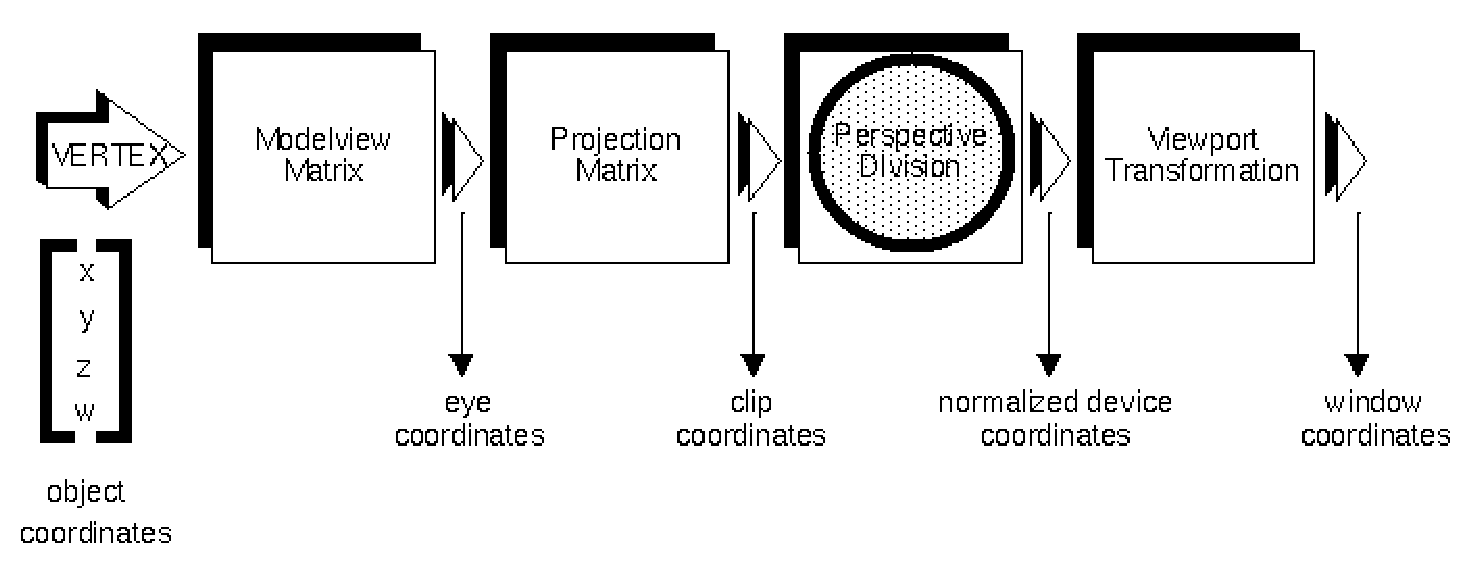
\includegraphics[height=5cm,
    angle=0]{./images/camera_view.eps}}
  \caption{Stages of Vertex transformation}
  \label{fig:camera_view}
\end{figure}


\begin{framed}
  \verb!gluPerspective()! is the GLU equivalent to
  \verb!glFrustum()!. \verb!gluOrtho2d! is the GLU equivalent to
  \verb!glOrtho()!.
\end{framed}

\begin{verbatim}
void gluPerspective(GLdouble  fFov, 
 	GLdouble  	fAspect, 
 	GLdouble  	fNear, 
 	GLdouble  	fFar);
\end{verbatim}
with \verb!fFov! is field-of-view angle, \verb!fAspect! is the aspect
ratio of the width to the height of the window (or the viewport),
\verb!fNear, fFar! are the distances from the eye (or virtual camera)
to the near and far clipping planes, Fig.~\ref{fig:perspective_2}.

\begin{figure}[hbt]
  \centerline{ 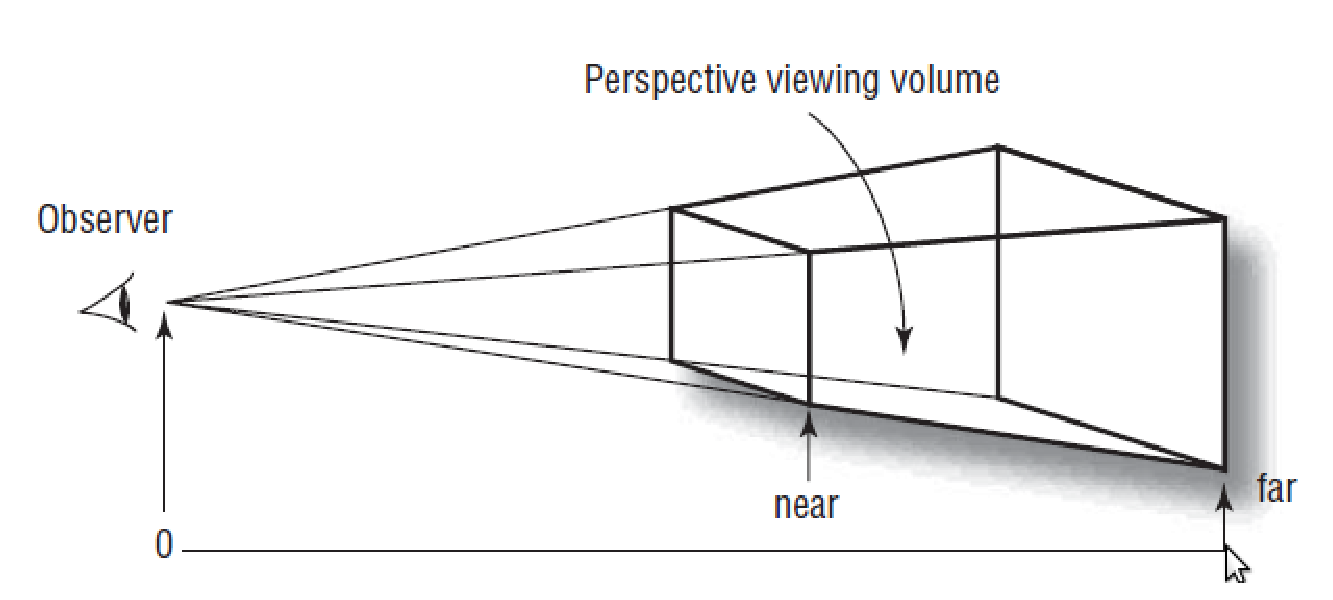
\includegraphics[height=4.5cm,
    angle=0]{./images/perspective_projection_2.eps}}
  \centerline{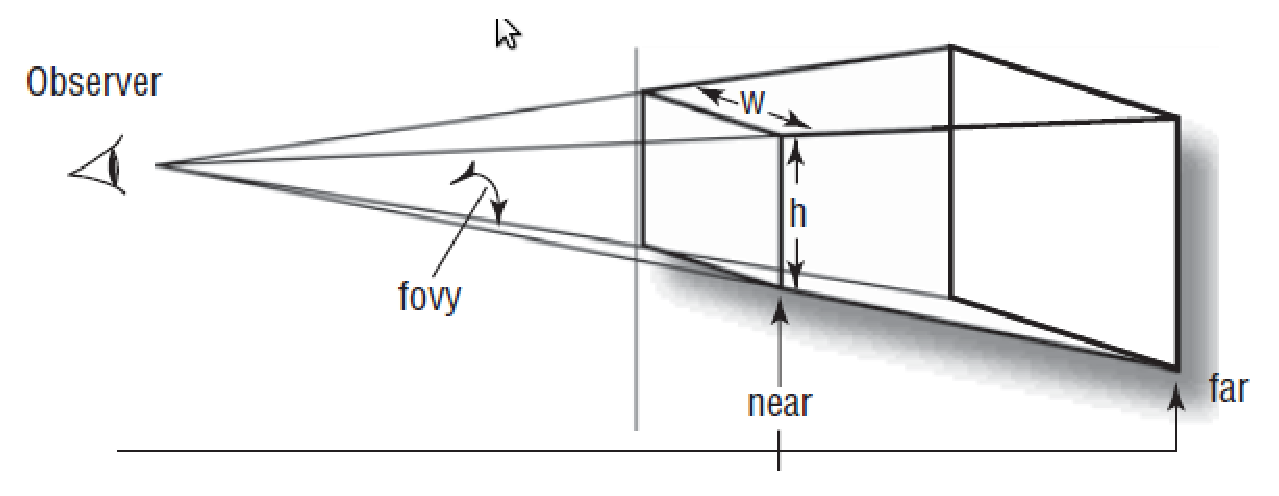
\includegraphics[height=3.8cm,
    angle=0]{./images/perspective_projection_3.eps}}
\caption{Perspective view}
\label{fig:perspective_2}
\end{figure}1

{\bf The question is how do we know what we plot fall inside this
  frustum?}. For example:
\begin{verbatim}
glBegin( GL_TRIANGLES );
glVertex2f( -0.5f, -0.5f, -10.0 );
glVertex2f( 0.5f, -0.5f, -10.0 );
glVertex2f( 0.0f, 0.5f, -10.0 );
glEnd();
\end{verbatim}
{\bf Frustum culling} is the technique that we need. There is no
OpenGL API or GLUT API to do this. However, it can be easily
implemented by
yourself\footnote{\url{http://www.opengl.org/resources/faq/technical/clipping.htm}}. 
\begin{enumerate}
\item We use a bounding sphere or cubeoid that just encloses all of
  the objects' vertices. This is called a 'bounding volume'.
\item And the question now is ``How do I tell if an arbitary sphere is
  either inside or crossing the six planes of the
  frustum?''\footnote{\url{http://www.sjbaker.org/steve/omniv/frustcull.html}} 
\end{enumerate}

\begin{framed}
  This describe frustum culling using cubeoid
  \begin{enumerate}
  \item Check if the z is more than the far plane value. If yes it can't
    be rendered. For eg:- if far = 50, anything with z < -50 ie z=-51
    and more will not be rendered

  \item Check if the z is less than near plane value. For eg:- near = 1,
    then anything above -1 will not render. So if z = 0 or z > 0 its
    outside the viewing volume

  \item Create a plane equation for left quad. Check if the triangle is
    inside the plane or not.

  \item Create a plane equation for right quad. Check if the triangle is
    inside or outside the plane.  Same goes for top and bottom.
  \end{enumerate}
\end{framed}


The question is when to use \verb!glOrtho!? It is typically used in
CAD application or for 2D graphics (e.g. 2D maps and onscreen head-up
displays).


Everything else needs to be done with the modelview matrix!

OpenGL has no notion of a "camera matrix" or world coordinate system.
The transformation after the modelview (i.e. model-to-view) coordinate
transformation has been applied your eye is in the origin of that
coordinate system (alas that's called eye-coordinate system).

To move your player forward you just transform the whole world in the opposite direction. Same for rotation of your player rotates to the left, just rotate the whole world to the right.

The only thing you need to consider for that is that the model- and
eye-coordinates are right handed in OpenGL Moving the player forward
means moving the world in +z-axis direction and so on...

\begin{verbatim}
//rendering a scene:
glMatrixMode(GL_PROJECTION);
glLoadIdentity();
glFrustum(...);
glMatrixMode(GL_MODELVIEW);
glLoadIdentity();
glRotatef(-cameraRoll, 0, 0, 1);
glRotatef(-cameraPitch, 1, 0, 0);
glRotatef(-cameraHeading, 0, 1, 0);
glTranslatef(-cameraPosition.x, -cameraPosition.y, -cameraPosition.z);

RenderWorld();   //static world

//repeat this for any movable object in the scene
glPushMatrix();
glTranslatef(objectPosision.x, objectPosision.y, objectPosision.z);
glRotatef(objectHeading, 0, 1, 0);
glRotatef(objectPitch, 1, 0, 0);
glRotatef(objectRoll, 0, 0, 1);
DrawObject();   //movable object
glPopMatrix();

\end{verbatim}

\begin{verbatim}
GLFrustum::SetOrthographic(GLfloat xMin, GLfloat xMax, GLfloat yMin,
            GLfloat yMax, GLfloat zMin, GLfloat zMax);

GLFrustum::SetPerspective(float fFov, float fAspect, 
                   float fNear, float fFar);
\end{verbatim}


\subsection{Off-screen rendering}
\label{sec:screen-rendering}

In the GPU pipeline, the traditional end point of every rendering
operation is the {\bf frame buffer}, a special chunk of graphics
memory from which the image that appears on the display is
read. Depending on the display settings (16bits, 24bits, or 32bits),
the most we can get is 32 bits of color depth, shared among the red,
green, blue and alpha channels of your display: Eight bits to
represent the amount of "red" in a image (same for green etc.: RGBA)
is all we can expect and in fact need on the display. Such
combinations already sums up to more than 16 million different
colors. 

Since we want to work with floating point values, 8 bits is clearly
insufficient with respect to precision. Another problem is that the
data will always be clamped to the range of [0/255; 255/255] once it
reaches the framebuffer. So, to create high-quality images, there is a
buffer - called {\bf offscreen buffer} which is an OpenGL extension
\verb!EXT_framebuffer_object! (aka {\bf FBO}) - that can be used as
the target of the rendering operations, providing full precision and
avoiding unwanted clamping issues.

\begin{framed}
  Why we need off-screen rendering?
  \begin{enumerate}
  \item generate intermediate images1 such as textures
  \item batch rendering of non-interactive animations
  \item high-resolution image generation for hard-copy, e.g. tiled
    rendering is a technique in which a large image is produced by
    tiling together smaller, individually rendered images. It's useful
    for generating images which are larger than what OpenGL would
    normally permit.
  \end{enumerate}
\end{framed}

Generally, off-screen rendering is not a core part of OpenGL. They are
provided as an extension such as GLX or
WGL\footnote{\url{http://www.mesa3d.org/brianp/sig97/offscrn.htm}}.  
\begin{enumerate}
\item Mesa provide OSMesa : off-screen rendering interfaces
\end{enumerate}

To use this extension and to turn off the traditional framebuffer and
use an offscreen buffer (surface) for our calculations, a few lines of
code suffice. 
\begin{verbatim}
GLuint fb;

void initFBO(void) {
    // create FBO (off-screen framebuffer)
    glGenFramebuffersEXT(1, &fb);
    // bind offscreen buffer
    glBindFramebufferEXT(GL_FRAMEBUFFER_EXT, fb);
}
\end{verbatim}


\begin{framed}
  Note that binding FBO number 0 will restore the window-system
  specific framebuffer at any time. This is useful for advanced
  applications but beyond the scope of this tutorial.
\end{framed}

Using FrameBuffer Object (FBO) is preferable for off-screen
rendering. For best performance, alternate rendering between two
different FBOs:
\begin{enumerate}
\item Render to A
\item Render to B
\item Read back from A and process it
\item Render to A
\item Read back from B
\item Goto 2
\end{enumerate}

Compared between rendering to a RenderBuffer vs. a Texture, rendering
to a renderbuffer is preferable. 


\section{Buffer objects (VBO vs. PBO vs. FBO)}
\label{sec:buffer-objects}

% \section{}
% \label{sec:vbo-vs.-pbo}

The power of graphics cards has been improved that can render meshes
with around 10 million vertices which requires hundreds of MB. The
main bottle neck now is the data bus for transmitting data from CPU
RAM to graphics card memory when processing data at this size, and the
transferring rate is high, e.g.  \verb!~!60 times per second across
the graphics bus. Traditional methods described in
Sect.~\ref{sec:interm-mode-vs} are no longer a good choice.


Besides drawing points, lines, polygons... (as shown in
Sect.~\ref{sec:interm-mode-vs}), in sect.~\ref{sec:arrays-=-textures},
we have learnt using texture to load image data for rendering. In this
section, we introduce a new technique to render and moving your data
around, as well as off-screen rendering. This can be done using
{\bf buffer objects}, and the data now can completely reside in
graphics memory.

Before OpenGL 3.2, you need to create hundreds of objects of varying
types. Now, we don't create geometric objects, we create buffer
objects. These buffer objects don't fix to a particular type of data,
i.e. it can reference to/hold vertex data, pixel data, texture data,
inputs for shader execution, or the output of different shader stages.

Create a new buffer object is simple, you can create a single or an
array of continuous buffer objects
\begin{verbatim}
!Fortran binding
INTERFACE
    SUBROUTINE glGenBuffers(n, buffers) BIND(C, name="glGenBuffers")
      USE iso_c_binding
      USE opengl_kinds
      INTEGER(Glsizei), VALUE:: n
      INTEGER(GLuint), DIMENSION(*) :: buffers
    END SUBROUTINE glGenBuffers

    SUBROUTINE glBindBuffer(n, buffer) BIND(C, name="glBindBuffer")
      USE iso_c_binding
      USE opengl_kinds
      INTEGER(GLenum), VALUE:: n
      INTEGER(GLuint), VALUE :: buffer
    END SUBROUTINE glBindBuffer
END INTERFACE
\end{verbatim}

\begin{verbatim}
Gluint pixBuffObjs[1];

glGenBuffers(1, pixBuffObjs);
\end{verbatim}
This will return you an integer value (the ID) - the name to the
buffer object. Each named buffer object can bind to a single target
and only one at a time. The target is known as the binding point, and
there are different types of them, as shown in
Table~\ref{tab:binding_point}. Each one serves a different purpose (to
be discussed shortly). 
\begin{verbatim}
glBindBuffer(GL_PIXEL_PACK_BUFFER, pixBuffObjs[0]);
\end{verbatim}

\begin{table}[hbt]
\begin{center}
\caption{Buffer object binding point}
\begin{tabular}{cp{7cm}} 
\hline
Target Name Description \\

\verb!GL_ARRAY_BUFFER! & Array buffers store vertex attributes such as color, position, texture
coordinates, or other custom attributes. \\
\verb!GL_COPY_READ_BUFFER! & Buffer used as the data source for copies with
glCopyBufferSubData. \\
\verb!GL_COPY_WRITE_BUFFER! & Buffer used as the target for copies
with glCopyBufferSubData. \\
\verb!GL_ELEMENT_ARRAY_BUFFER! & Index array buffer used for sourcing indices for glDrawElements,
glDrawRangeElements, and glDrawElementsInstanced. \\
\verb!GL_PIXEL_PACK_BUFFER! & Target buffer for pixel pack operations
such as glReadPixels. \\
\verb!GL_PIXEL_UNPACK_BUFFER! & Source buffer for texture update functions such as glTexImage1D,
glTexImage2D, glTexImage3D, glTexSubImage1D,
glTexSubImage2D, and glTexSubImage3D. \\
\verb!GL_TEXTURE_BUFFER! & Buffer accessible to shaders through texel
fetches. \\
\verb!GL_TRANSFORM_FEEDBACK_BUFFER! & Buffer written to by a transform
feedback vertex shader. \\
\verb!GL_UNIFORM_BUFFER! & Uniform values accessible to shaders. \\
\hline\hline
\end{tabular}
\end{center}
\label{tab:binding_point}
\end{table}


After binding a named buffer to target, we need to fill valid data
into it (i.e. filling the buffer)
\begin{verbatim}
// named buffer must be bound before calling this
glBufferData(GL_PIXEL_PACK_BUFFER, pixelDataSize, pixelData,
              GL_DYNAMIC_COPY);

\end{verbatim}

\begin{enumerate}
\item Pixel buffer objects are a great container for temporarily
  storing pixel data locally on the GPU, but remember they need to
  have storage allocated before they can be
  used.(Sect.~\ref{sec:pbo}). 

\item Just like all other buffer objects, calling \verb!glBufferData!
  allocates storage for a buffer and fills it with your data. But you
  don't necessarily have to provide data; passing in NULL for the data
  pointer simply allocates the memory without filling it.

\item If you don't allocate storage for a buffer before trying to fill
  it, OpenGL throws an error.
\end{enumerate}

\begin{framed}
  Note that this pointer to the third argument of
  \verb!glBufferData()! can also be NULL if you want to allocate a
  buffer of a specific size but do not need to fill it right away. The
  fourth parameter of \verb!glBufferData()! is where you tell OpenGL
  how you intend to use the buffer.
\end{framed}


Using \verb!GL_DYNAMIC_DRAW! is a safe value for general buffer usage
or situations where you aren't sure what the buffer will be used for
(read more later).  With that, you can always call \verb!glBufferData!
again, refilling the buffer and possibly changing the usage
hint. Recalling glBufferData, however, wipe out all data, to update
the new one. If only a small fraction of the data change, you can
improve the performance by telling OpenGL with
\verb!glBufferSubData()! to update a part of a preexisting buffer
without invalidating the contents of the rest of the buffer.

\begin{verbatim}
void glBufferSubData(GLenum target, intptr offset, 
                     sizeiptr size, const void *data);
\end{verbatim}
The \verb!offset! tell the offset (in bytes) from the beginning of the
buffer from which the update start. However, using
\verb!glBufferSubData()!, we cannot change the usage of the buffer,
e.g. change from \verb!GL_DYNAMIC_DRAW! to some thing else. 

When you are finished with a buffer, it needs to be cleaned up, just
as all other OpenGL objects should be. First, you need to unbind the
buffer, before you can delete the buffer.
\begin{verbatim}
// unbind the buffer: use the same binding point, with 
// the second argument is ``0'' 
glBindBuffer(GL_PIXEL_PACK_BUFFER, 0);

// make sure you unbound the buffer before delete it
glDeleteBuffers(1, pixBuffObjs);
\end{verbatim}
The unbound buffer can later bind to any other binding point. 



{\bf SUMMARY}: 
\begin{verbatim}
 // generate a VBO object
id = glGenBuffers(1)
 // tell what kind of data that VBO object
 // will reference to
glBindBuffer(target, id)

 // put the data to the buffer, along with tell how
 // often the data is modified
glBufferData(target, size, data, usage)
\end{verbatim}
with \verb!target! is one of those given in Table
\ref{tab:binding_point}., \verb!size! is the number of bytes to
transfer. \verb!data! is the big array containing the source data.

The \verb!usage! tell how often the data is updated/modified. There
are 3 modes of usage, with total 9 transfer modes (the first three
modes to support are \verb!GL_..._DRAW!)

\begin{itemize}
\item STATIC = specify the data only once, and use it many times
  without modifying it
  \begin{itemize}
  \item \verb!GL_STATIC_READ!
  \item \verb!GL_STATIC_COPY!
  \item \verb!GL_STATIC_DRAW! when vertex data never or almost never
    updated)
  \end{itemize}

  Data are sent only once from the CPU to the graphics card where they
  are saved in the graphic controller memory
  (\textcolor{red}{so it provides the highest performance}). This mode
  is suitable for non-deformable objects which remains unchanged
  during several frames

\item STREAM = modify the data once, then use it once, and repeat the
  process many time
  \begin{itemize}
  \item \verb!GL_STREAM_READ! 
  \item \verb!GL_STREAM_COPY!
  \item \verb!GL_STREAM_DRAW! when vertex data could be updated
    between each rendering)
  \end{itemize}

  This mode is particularly useful for CPU animated objects, i.e. data
  are sent each call to glDrawArrays, glDrawElements,
  glDrawRangeElements (\verb!EXT_draw_range_elements!, OpenGL 1.2)
  glMultiDrawArrays or glMultiDrawElements
  (\verb!EXT_multi_draw_array!, OpenGL 1.4).


\item DYNAMIC = specify/modify the data repeatedly, and use it
  repeatedly. 
  \begin{itemize}
  \item \verb!GL_DYNAMIC_READ! 
  \item \verb!GL_DYNAMIC_COPY!
  \item \verb!GL_DYNAMIC_DRAW! when vertex data could be updated
    between each frames
  \end{itemize}
  
  In this mode, the graphics driver will in charge of choosing the
  data location.
  \textcolor{red}{This mode is recommended for animated object that
    require rendering several time per frame}
\end{itemize}


\begin{framed}
  Mode \verb!GL_*_DRAW! provides the same behavior as Vertex Arrays
  (but used with glDrawArrays, glDrawElements, glDrawRangeElements,
  glMultiDrawArrays or glMultiDrawElements)

  Mode \verb!GL_..._READ!  allows you to read data managed by OpenGL.

  Mode \verb!GL_*_COPY!  allow displaying geometric from source
  managed by OpenGL.
\end{framed}
% With VBO, the OpenGL APIs tell the card to use the stored data instead
% of client-side vertex-sets when we want to render our geometry using
% array-based operations. This is the same basic operation we've done
% with textures and display lists. We store the data on the card
% identified by a unique ID for later reference and trigger its use when
% we would normally re-transfer the data.

% You can delete a single VBO or multiple VBOs with glDeleteBuffer(s) if
% they are not used anymore. After a buffer object is deleted, its
% contents will be lost.


\begin{framed}
  \verb!glMapBuffer! is synchronous mapping.  To avoid waiting (idle),
  you can call first glBufferDataNull, then call glMapBuffer. In this
  case, the previous data will be discarded and glMapBuffer returns a
  new allocated pointer immediately even if GPU is still working with
  the previous data.

  However, this method is valid only if you want to update entire data
  set because you discard the previous data. If you want to change
  only portion of data or to read data, you better not release the
  previous data.

\end{framed}


\subsection{VBO}
\label{sec:vbo}

Vertex buffer object (VBO) is an extension in OpenGL 1.4 and become
the standard in OpenGL
1.5\footnote{ VBOs are also available with OpenGL ES 2.0 but this
  feature is optional.}.
So, all OpenGL APIs working with VBO in OpenGL 1.4 should be prefixed
with \verb!ARB!, e.g. \verb!glGenBuffersARB()!.
\textcolor{red}{``Features, efficiency and longevity are three reasons
  to use VBOs as soon as possible''}.

VBO are buffers into which we can load vertex array data
(Sect.~\ref{sec:vertex-arrays}), as well as color, normal, and face
indexing data. These data can reside in high-performance graphics
memory, i.e. the server side, and thus promotes efficient data
transfer. 
\begin{itemize}
\item Color, normal and coordinate arrays are passed as 'just array
  buffers' \verb!GL_ARRAY_BUFFER!, and use glColorPointer(),
  glVertexPointer(), glNormalPointer() for rendering.

\item Indexed faces are passed using element array buffers
  \verb!GL_ELEMENT_ARRAY_BUFFER!, and use glDrawElements() for rendering.
\end{itemize}

\begin{framed}
  VBO (Vertex Buffer Objects (Arrays)) is a techniques that OpenGL use
  to connect to geometry (vertex) data that reside in ``fast'' memory
  (i.e. video RAM). Though we can associate the data with a VBO
  object, the actual storage location of the data is hidden from you.

  VBO are similar in principles to PBO but provide lots of
  improvements with 3 transfer modes (i.e. access pattern) compared to
  using PBO. We use VBO to generate 3D meshes and utilize OpenGL VBOs
  (Vertex Buffer Objects) to efficiently render meshes as a colored
  surface, wireframe image or set of 3D points.

% \begin{verbatim}
% glGenBuffersARB
% glBindBufferARB
% glDeleteBufferARB
% ..
% ..
% (and so on)
% \end{verbatim}
\end{framed}

% VBO code looks pretty much like regular OpenGL 1.1 array-using
% code. You build the same arrays, but instead of passing the arrays
% into OpenGL, you set up a VBO object and load the data into it. A VBO
% object is simply an integer or an array of integers that we use to get
% reference to data residing on the server side (i.e. graphics card
% memory).
\textcolor{red}{Creating a VBO requires these functions}:

\begin{itemize}
\item \verb!glGenBuffers()!: create one or a continuous array of VBOs
  (handle variable)
\begin{verbatim}
GLvoid glGenBuffers(GLsizei n, GLuint* buffers);
\end{verbatim}
  with $n$ is the number of VBO objects, $buffers$ is an integer array
  (or a scalar) keeping the VBO objects' IDs.  

\item \verb!glBindBuffer()!: active the buffer (or make the handle
  ``current''). Here, instead of addressing the memory using pointer,
  we address buffers using handle. This buffer will later be loaded
  with data

\item\verb!glBufferData()!, or \verb!glBufferSubData()!: copy
  vertex/color/normal/ data to the buffer: which are conceptually
  similar to \verb!glTexImage*()! and \verb!glTexSubImage*()!.
  \begin{itemize}
  \item call \verb!glBufferData()! to get a pointer to the VBO (with
    desired mode: \verb!GL_READ_ONLY, GL_WRITE_ONLY, GL_READ_WRITE!),
    then write data to it, and finish by calling
    \verb!glUnmapBuffer()!

  \end{itemize}

\item \verb!glDeleteBuffers()!: delete the buffer
\begin{verbatim}
GLvoid glDeleteBuffers(GLsizei n, const GLuint* buffers);
\end{verbatim}

\end{itemize}
If you use \verb!glBufferDataNull! instead, then no data parameter is
provided and then VBO reserves only memory space with the given data
size. 

{\bf Example}:
\begin{enumerate}
\item Call this code (or similar) ONCE (i.e. not inside the callback)
  for each array you want to buffer
\begin{verbatim}
// this example illustrates how to load a vertex array buffer.
// only small variations for loading color arrays
// and element (indexed triangle) arrays.
// see the rest of the article for details.
// create a handle that you will use to refer to the buffer when talking to gl
GLuint handle;
glGenBuffers(1,&handle);
// let's load our buffer data...
// size of your buffer, here, 3 times the number of vertices,
// multiplied by your format size, for example sizeof(GL_FLOAT).
int dataByteSize = ...
float* data = malloc(dataByteSize)
// need to populate your buffer with vertex data!
...
// this loads 'data' into graphic memory referred by 'handle'
glBindBuffer(GL_ARRAY_BUFFER,handle);
// Typically you want to use static draw. This implies you will use the buffer
// over and over, in other words you won't modify geometry afterwards.
glBufferData( GL_ARRAY_BUFFER, dataSize, data, GL_STATIC_DRAW);
// clear the binding after loading your array, otherwise you will get crashes
glBindBuffer(GL_ARRAY_BUFFER,0);
\end{verbatim}

\item Put this inside the callback (rendering)
\begin{verbatim}
// this example illustrates how to 'pass pointers' with
// 'pass array buffers'
// note: this example only makes sense if you can do basic gl rendering.
glBindBuffer(GL_ARRAY_BUFFER,handleToColorBuffer);
glVertexPointer(4,GL_FLOAT,0,0 /*replaced the pointer reference by zero*/ );
glBindBuffer(GL_ELEMENT_ARRAY_BUFFER,handleToPerFaceVertexIndices);
glDrawElements(... , 0 /*replaced the pointer reference by zero*/ );
\end{verbatim}

\end{enumerate}

{\bf Example}: draw a cube
\begin{enumerate}
\item Allocate the new buffer
\begin{verbatim}
// allocate a new buffer
glGenBuffers(1, &cubeVBO);
// bind the buffer object to use
glBindBuffer(GL_ARRAY_BUFFER, cubeVBO);
\end{verbatim}

\item Normally, the data involve vertex and color information. 
\begin{verbatim}
const GLsizeiptr vertex_size = NUMBER_OF_CUBE_VERTICES * &
       NUMBER_OF_CUBE_COMPONENTS_PER_VERTEX*sizeof(GLfloat);
const GLsizeiptr color_size = NUMBER_OF_CUBE_COLORS * &
       NUMBER_OF_CUBE_COMPONENTS_PER_COLOR*sizeof(GLubyte);
\end{verbatim}

\item Copy the data to the VBO object, and tell how often we want to
  modify the data (this will help OpenGL works  better)
\begin{verbatim}
// allocate enough space for the VBO
glBufferData(GL_ARRAY_BUFFER, vertex_size+color_size, 0, GL_STATIC_DRAW);
\end{verbatim}
  We have two different pieces of data, the vertices and the
  colors. For this case, \verb!glBufferSubData! is one way of copying
  sections of data into the buffer. Another way is to use
  \verb!glMapBuffer!. At a high level, glMapBuffer is sort of like
  direct memory access (DMA) for your video card. It potentially
  avoids an extra system copy by creating a direct map of memory.

  For example, we use glMapBuffer
\begin{verbatim}
GLvoid* vbo_buffer = glMapBuffer(GL_ARRAY_BUFFER, GL_WRITE_ONLY_OES);
	// transfer the vertex data to the VBO
	memcpy(vbo_buffer, s_cubeVertices, vertex_size);

	// append color data to vertex data. To be optimal,
	// data should probably be interleaved and not appended
	vbo_buffer += vertex_size;
	memcpy(vbo_buffer, s_cubeColors, color_size);
glUnmapBuffer(GL_ARRAY_BUFFER); 
\end{verbatim}
  As you can see, color information cluster at one place, vertex
  information cluster at another place. This makes the copying
  straightforward, though is not recommended, as OpenGL prefer
  interleaved data, i.e. vertex data, color data, vertex data, color
  data... This will allow drawing a single point faster as it can
  easily and quickly obtain the location and color information of that
  point. This is particularly important if we have more information
  \textcolor{red}{(position, color, texture coordinates, normals)}.

\item After the VBO object has referenced/mapped to the data, we need
  to tell how the data is organized (as in the beginning OpenGL only
  know this is a chunk of byte)
\begin{verbatim}
// Describe to OpenGL where the vertex data is in the buffer
/* we tell OpenGL we have vertices with 
       - 3 components per vertex (x, y, x) 
       - and they are GL_FLOATs. 
       - stride = 0
       - starting from the beginning of the array. 
*/
glVertexPointer(3, GL_FLOAT, 0, (GLvoid*)((char*)NULL));

// Describe to OpenGL where the color data is in the buffer
/* For the color data where we have 
       - 4 components (R, G, B, A)
       - each is GL_UNSIGNED_BYTEs
       - stride = 0
       - and start in the array position after the vertex points.
*/
glColorPointer(4, GL_UNSIGNED_BYTE, 0, & 
              (GLvoid*)((char*)NULL+vertex_size));
\end{verbatim}
  If you have texture coordinates or normals, don't forget to use
  glTexCoordPointer and glNormalPointer in the same
  way. \textcolor{red}{The order of calling these functions are
    important}. 

\item Now, we still need an index array (some people call this Index
  Buffer Objects (IBOs)) and now we use \verb!GL_ELEMENT_ARRAY_BUFFER!
  instead of \verb!GL_ARRAY_BUFFER! in our call to glBindBuffer. This
  is what distinguishes the IBO from the VBO.
\begin{verbatim}
// create index buffer
glGenBuffers(1, &cubeIBO);
glBindBuffer(GL_ELEMENT_ARRAY_BUFFER, cubeIBO);

/* For constrast, instead of glBufferSubData and glMapBuffer,
   we can directly supply the data in one-shot, i.e. pass the
   data when you first allocate the memory. We can do this as
   we don't need to combine separate arrays (like for vertex 
   and color)
*/
glBufferData(GL_ELEMENT_ARRAY_BUFFER, & 
     NUMBER_OF_CUBE_INDICES*sizeof(GLubyte), & 
     s_cubeIndices, GL_STATIC_DRAW);
\end{verbatim}

\item At this point, we can render
\begin{verbatim}
// Activate the VBOs to draw
glBindBuffer(GL_ARRAY_BUFFER, cubeVBO);
glBindBuffer(GL_ELEMENT_ARRAY_BUFFER, cubeIBO);

glEnableClientState(GL_VERTEX_ARRAY);
glEnableClientState(GL_COLOR_ARRAY);

/* This is the actual draw command
  Without it, nothing will be drawn.
*/
glDrawElements(GL_TRIANGLE_STRIP, NUMBER_OF_CUBE_INDICES, &
       GL_UNSIGNED_BYTE, (GLvoid*)((char*)NULL));
\end{verbatim}
  We bind the buffers. We tell the system we want to draw vertices and
  colors. (We don't have normals and texture coordinates in this
  example, but if we did we would also need to enable
  \verb!GL_NORMAL_ARRAY! and \verb!GL_TEXTURE_COORD_ARRAY!.)

\item Before we exit, we need to clean up the resource
\begin{verbatim}
glDeleteBuffers(1, &cubeIBO);
glDeleteBuffers(1, &cubeVBO);
\end{verbatim}
\end{enumerate}
\url{http://playcontrol.net/ewing/jibberjabber/opengl_vertex_buffer_object.html} 


VBO are unformatted objects, i.e. they are a big chunk of bytes. Thus,
OpenGL doesn't care whether they contain float data, what the ordering
is ... until you call a ``draw'' function. Rendering a VBO is almost
similar to rendering the array. Therefore, no additional APIs are
required to draw VBO except glBindBuffer.
\begin{verbatim}
// bind VBOs for vertex array and index array
glBindBuffer (GL_ARRAY_BUFFER, vboId1);//  (* for vertex coordinates *)
glBindBuffer (GL_ELEMENT_ARRAY_BUFFER, vboId2);// (* for indices *)

//(* do same as vertex array except pointer *)
glEnableClientState (GL_VERTEX_ARRAY);//(* activate vertex coords array *)
glVertexPointer(3, GL_FLOAT, 0, 0); // (* last param is offset, not ptr *)

//(* draw 6 quads using offset of index array *)
glDrawElements GL_QUADS 24 GL_UNSIGNED_BYTE 0;

glDisableClientState GL_VERTEX_ARRAY;  //(* deactivate vertex array *)

(* unbind, so switch back to normal pointer operation *)
glUnbindBuffer GL_ARRAY_BUFFER;
glUnbindBuffer GL_ELEMENT_ARRAY_BUFFER;
\end{verbatim}

% Like glBufferData, glBufferSubData is used to copy data into VBO, but
% it only replaces a range of data into the existing buffer, starting
% from the given offset. (The total size of the buffer must be set by
% glBufferData before using glBufferSubData.)  


We can update VBO data (which can not be done with
{\bf display list}).
\begin{enumerate}
\item the simplest way: copy new data into the bound VBO with
  glBufferData or glBufferSubData. Here, we need 2 copies of vertex
  data: one in your application and one in your VBO, then we can
  switch between them. 

\item
  \textcolor{red}{ The second improvement that characterise VBO sis
    called Vertex mapping (see CUDA-OpenGL)}.  Instead of telling
  OpenGL to copy the data into the VBO buffer, we can tell it to
  temporarily map buffer object into client's memory, then the
  client can update the data with a pointer to the mapped buffer
  using \verb!glMapBuffer!. This is similar to that being used in
  CUDA-OpenGL interop, when we map buffer object to CUDA memory
  space.
\begin{verbatim}
glMapBuffer(target, access, ...)
\end{verbatim}
  with access can be
\begin{verbatim}
GL_READ_ONLY
GL_WRITE_ONLY
GL_READ_WRITE
\end{verbatim}

  After that, unmapped the data from client's memory, to avoid it being
  modified by any other process.
\end{enumerate}


VBOs provide an excellent alternative to interleaved arrays. As a
recalling, interleaved arrays allow sending vertices data to the
graphics card using a single array decribes by the function
\verb!glInterleavedArrays!. With vertex arrays, we must using
predefined data structures with defined order for each element of this
structure. With GPU programming arising, programmer custom attributes
aren't managed by this solution. VBOs solve this issue and allow
updated of only a part of the data.


\subsection{PBO}
\label{sec:pbo}

{\bf Pixel Buffer Objects} (PBO) is not new. Pixel buffer objects are
similar to texture buffer objects in that they hold pixel/texel data;
yet the data now reside on GPU.

Possible binding targets for PBO are
\begin{verbatim}
GL_PIXEL_PACK_BUFFER
    When a PBO is attached to this target, 
    any OpenGL operations that "read" pixels get their data from the PBO
 -> glReadPixels, glGetTexImage, and glGetCompressedTexImage
  
GL_PIXEL_UNPACK_BUFFER
    any OpenGL operations that "draw" pixels put their data 
    into an attached PBO.
 -> glTexImage*D, glTexSubImage*D, glCompressedTexImage*D,
      and glCompressedTexSubImage*D.


\end{verbatim}

All calls to \verb!glBufferData()! are pipelined with the rest of your
draw calls. That means the OpenGL implementation won't have to wait
for all activities to stop before sending the new data to the GPU.

\begin{framed}
  Pixel buffers are often used to hold 2D images coming from a
  renderbuffer target, texture, or other source.
  \textcolor{red}{However, buffer objects are one-dimensional by
    nature; they don't have an intrinsic width or height}.
  When allocating storage space for 2D images, you can just multiply
  the width by the height by the size of a pixel.

    If you plan to use the same PBO for multiple data sizes, you are
    much better off sizing the PBO for the largest data set right away
    than resizing it frequently.
\end{framed}

We use PBO to create images with CUDA on a pixel-by-pixel basis and
display them using OpenGL. PBO (Pixel Buffer Objects) is not a new
OpenGL object (added to OpenGL 2.1). It just says ``we can use the
buffer object for pixel operations, not just geometry operations''.


After you render the frame, i.e. the data is sent to renderbuffer, you
may want to read the data \textcolor{red}{ back to client memory},
e.g. use the data from previous frames to apply the effect on the next
frame. To do so, we use \verb!glReadPixels()! (to read back to GPU
memory, read the solution later)
\begin{verbatim}
void* data = (void*)malloc(pixelDataSize);
glReadBuffer(GL_BACK_LEFT);
glReadPixels(0, 0, GetWidth(), GetHeight(), GL_RGB, GL_UNSIGNED_BYTE, pixelData);
\end{verbatim}
Before reading back to client memory, the entire pipeline often has to
be emptied to ensure all drawing that would affect the pixels you are
about to read has completed.  This can have a major impact on your
application's performance. But the good news is we can use buffer
objects to overcome this performance issue. You can bind a buffer
object to the \verb!GL_PIXEL_PACK_BUFFER! before you call glReadPixels
and set the data pointer in the glReadPixels call to null. This
redirects the pixels into a buffer located on the GPU and avoids the
performance issues that copying to client memory can cause.
\begin{verbatim}
glReadBuffer(GL_BACK_LEFT);
glBindBuffer(GL_PIXEL_PACK_BUFFER, pixBuffObjs[0]);
glReadPixels(0, 0, GetWidth(), GetHeight(), GL_RGB, GL_UNSIGNED_BYTE, NULL);
\end{verbatim}

\subsubsection{Blur effect}
\label{sec:blur-effect}

What we can do 
\begin{enumerate}
\item An application can render multiple times to a buffer, slightly
  offsetting the fast moving objects and blending the results
  together. 
\item Another option is to sample texel data for an object image
  multiple times in the direction of movement and then blend the
  sample results together. 
\item There are even more involved methods that use depth buffer data
  to apply a more dramatic blur to objects closer to the camera.  

\item A simple approach is stores the results of previous frames and
  blends them together with the current frame
\end{enumerate}

Simple approach: we use texture and PBO. Here, 6 textures units are
used for blur effect. Here, we dont use swap; the result is copied
into a texture to be used for the blur effect.
\begin{verbatim}
// Create blur textures
  glGenTextures(6, blurTextures);
// Allocate a pixel buffer to initialize textures and PBOs
  pixelDataSize = GetWidth()*GetHeight()*3*sizeof(unsigned byte);
  void* data = (void*)malloc(pixelDataSize);
  memset(data, 0x00, pixelDataSize);
// Setup 6 texture units for blur effect
// Initialize texture data
for (int i=0; i<6;i++)  {
  glActiveTexture(GL_TEXTURE1+i);
  glBindTexture(GL_TEXTURE_2D, blurTextures[i]);
  glTexParameteri(GL_TEXTURE_2D, GL_TEXTURE_WRAP_S, GL_CLAMP_TO_EDGE);
  glTexParameteri(GL_TEXTURE_2D, GL_TEXTURE_WRAP_T, GL_CLAMP_TO_EDGE);
  glTexParameteri(GL_TEXTURE_2D, GL_TEXTURE_MIN_FILTER, GL_LINEAR);
  glTexParameteri(GL_TEXTURE_2D, GL_TEXTURE_MAG_FILTER, GL_LINEAR);
  glTexImage2D(GL_TEXTURE_2D, 0, GL_RGB, GetWidth(), GetHeight(), 0, GL_RGB,
                 GL_UNSIGNED_BYTE, data);
}

// Allocate space for copying pixels so we don't call malloc on every draw
glGenBuffers(1, pixBuffObjs);
glBindBuffer(GL_PIXEL_PACK_BUFFER, pixBuffObjs[0]);
glBufferData(GL_PIXEL_PACK_BUFFER, pixelDataSize, pixelData, GL_DYNAMIC_COPY);
glBindBuffer(GL_PIXEL_PACK_BUFFER, 0);
\end{verbatim}
If texture 3 was used last time, texture 4 will be used next. That
means texture 4 will contain data from this frame, texture 3 from the
last, texture 2 from two frames ago, and so on.

The target for the current frame wraps around again after the last
texture has been used. The pixel data for the last six frames is
always ordered and available in this 'texture ring buffer'.For the
traditional path, this happens by calling glReadPixels to get the
pixel data and then glTexImage2D to move the pixel data into a texture
object.

\begin{framed}
  On slower systems the PBO path is almost six times faster than the
  client memory path.
\end{framed}
The PBO path is slightly different. Instead of copying the data back
to the CPU, the PBO is bound to the \verb!GL_PIXEL_PACK_BUFFER!, and
when we call glReadPixels, the pixels are redirected to the PBO
instead of back to the CPU. Then that same buffer is unbound from the
\verb!GL_PIXEL_PACK_BUFFER! attachment and bound to the
\verb!GL_PIXEL_UNPACK_BUFFER!. When glTexImage2D is called next, the
pixel data in the buffer is loaded into the texture, all without ever
leaving the GPU and remaining pipelined with other OpenGL commands.
You can see this process in Listing 8.2. Finally, the ring buffer is
updated to point to the next blur texture. You can press the P button
while running the program to switch between the two paths.

\subsection{TBO }
\label{sec:tbo-}

Texture Buffers allow you to do many things that traditional buffers
cannnot do. 

\subsection{FBO}
\label{sec:fbo}


Normally, rendering write out the graphics to a window or the full
screen. So, a default framebuffer object is created and bound to the
window automatically when an OpenGL context is created.  Now, OpenGL
give you the option to create multiple framebuffer objects (FBO) and
you can render to these FBO, instead to the framebuffer bound to the
window. This is known as {\bf off-screen rendering}
(Sect.~\ref{sec:screen-rendering}.

FBO is a new and better choice. It replaces previous render-to-texture
methods (e.g. offscreen window, PBuffers) (added to OpenGL 3.0). FBOs
are not limited to the size of the window and can contain multiple
color buffers, i.e. allow rendering high resolution output.
\begin{framed}
  Framebuffers are not really buffers, i.e. there is no real memory
  storage associated with a framebuffer object (FBO). Instead, FBOs
  are containers that can hold other objects that do have memory
  storage and can be rendered to, such as textures or renderbuffers. 

  So, before we can render to an FBO, we have to add images
\end{framed}


\begin{framed}
  MIP maps (or {\bf mipmaps}) are pre-calculated, optimized set of
  images (i.e. sequence of textures), each is a progressively lower
  resolution representation of the same image, that accompany a main
  texture that help increase the rendering speed and reduce
  antialiasing.

  Normally, the image in the main texture is of largest size
  (e.g. 256x256), and the images in the mipmaps set is the smaller
  sizes (128x128, 64x64, 32x32, 16x16...).  By keeping multiple copies
  at different level of detail, the render can switch to the suitable
  mipmap image when the texture is viewed from a distance or at a
  smaller size.

  In some cases, we may want the images in the mipmaps set to be
  nonuniform compared to the main texture, known as {\bf ripmaps},
  e.g. 128x64, 128x32, ... However, ripmaps are unpopular due to
  higher memory demand. 
\end{framed}

When we draw, we often need an RGBA image buffer and a 32-bit depth
buffer that is separate (or may be there are other buffers too). FBO
allows drawing into RGBA texture and DEPTH-type buffers at the same
time.  

\subsection{Reading data from buffer objects}
\label{sec:reading-data-from}

The previous sections tell you how to load data into a target-bound
named buffer. Now, we will learn how to read the data back which may
be helpful in some cases.

We'll takes pixels from the currently enabled read buffer and copies
them into local CPU memory
\begin{verbatim}
void* data = (void*)malloc(pixelDataSize);
glReadBuffer(GL_BACK_LEFT);
glBindBuffer(GL_PIXEL_PACK_BUFFER, pixBuffObjs[0]);

glReadPixels(0, 0, GetWidth(), GetHeight(), 
            GL_RGB, GL_UNSIGNED_BYTE, pixelData);
\end{verbatim}


\section{OpenXX}
\label{sec:openxx}

There are many Open-standard being used nowadays
\begin{itemize}
\item OpenCL (Open Computing Language) = lower level of CUDA
\item OpenAL (Open Audio Library) = cross-platform audio APIs
\item OpenML (Open Media Library) = cross-platform programming
  environment for capturing, transporting, processing, displaying, and
  synchronizing digital media (2D/3D graphics, audio \& video, I/O,
  networking) 
\item OpenSL ES (Open Sound Library for Embedded Systems) = C-language
  audio API for 2D/3D audio being used in mobile and gaming industry. 
\end{itemize}

Read more on Chap.~\ref{chap:cuda-opengl}. 

\chapter{Mesa}
\label{chap:mesa}
\label{sec:mesa}


Mesa is a term used to encompass the different open source graphics drivers
available on Linux, so it can be what powers your GPU. 
Mesa itself is not a driver, as you will be using a different part of Mesa for
each graphics card vendor.  

Nowadays, we call it Mesa3D, it implements 3D graphics library
(Sect.\ref{sec:mesa-3d})

Originally, Mesa began only to serve as an open source Linux implementation of
OpenGL (Chap.\ref{chap:opengl}), but it has since grown to be a lot more than
that. Mesa implements various API's (Application programming interface) like
OpenGL, OpenGL ES, OpenCL, OpenMAX, VDPAU, VA API, XvMC and Vulkan.


Mesa was started in 1993 by Brian Paul (for freedesktop.org), but now it has
many more developers, some of which are employed by the likes of AMD, Intel,
Valve and others.
Linux game porters like Feral Interactive have also contributed code to Mesa.
Plenty of people also help with Mesa development in their spare time too.

\section{Mesa driver}

You may not using Mesa driver, depending upon the GPU device
\begin{enumerate}
  \item Intel HD Graphics card: you must be using Mesa

Exception: Intel usually supports Mesa quite well and even have their own Mesa
update tool named 'Intel Graphics Update Tool' to give certain distributions
the latest version of Mesa. 
 
  \item AMD GPU:   most AMD graphics cards have pretty good support in Mesa,
  with the closed source driver often not being needed.

The latest AMD cards use the \verb!amdgpu! kernel driver (the proprietary
AMDGPU-PRO also uses a version of this, which has not yet been accepted into the
Linux kernel yet), whereas all older cards use the \verb!radeon! kernel driver.
Each part of Mesa listed below hooks into one of those kernel drivers.

\begin{verbatim}
radeon - R100 series
r200 - R200 series
r300g - R300, R400, and R500 series
r600g - R600, R700, HD 5000 and HD 6000
radeonsi - HD 7000, HD 8000 and RX 200, RX 300 and RX 400

You also have the 'radv' driver for Vulkan, which was officially added in Mesa
13. It's still in development right now, so it's to be considered in beta.  
\end{verbatim}
  
  \item Nvidia GPUs: For NVIDIA, it's usually best to stick with the proprietary
  driver, ie. dont' use Mesa. 

 
  NVIDIA doesn't help towards development of Mesa, since they prefer their own
  closed-source proprietary drivers. For NVIDIA cards Mesa is typically quite
  far behind the closed drivers in terms of performance and features due to
  this. Mesa also typically doesn't work well, if at all with the very latest
  generation of NVIDIA graphics cards.   



With Mesa, you have the nouveau (pronounced like nu-vo) kernel driver, but like
AMD, NVIDIA uses nouveau plus another part of Mesa depending on your graphics
card model.

Later generations of NVIDIA cards require something called 'signed firmware' in
order for Mesa to interact with them and NVIDIA has been quite slow to release
it. The 'Pascal' generation in particular right now has very little support, as
NVIDIA has only recently provided the signed firmware required.
  
\end{enumerate}
\url{https://www.gamingonlinux.com/articles/an-explanation-of-what-mesa-is-and-what-graphics-cards-use-it.9244}

Versioning:
\begin{verbatim}
glxinfo | grep Mesa
\end{verbatim}

Get the latest {\it stable} Mesa driver for AMD and Intel
\begin{verbatim}
sudo add-apt-repository ppa:paulo-miguel-dias/pkppa
sudo apt-get update


\end{verbatim}

We need
\begin{verbatim}
Mesa 9.1.3
   GLproto 1.4.16
      util-macros-1.17 (ignore what 'make' tell you)
      libdrm-2.4.24+ (.36, .42)
      dri2proto-2.8 (modify configure.ac bloack XORG...)
  libxcb-1.9
      xcb-proto-1.8
  libtool-2.4.2
  pkg-config-0.27.1
  automake-1.12

Mesa 9.0.3
   GLproto 1.4.16
      util-macros-1.17 (ignore what 'make' tell you)
      libdrm-2.4.24+ (.36, .42)
      dri2proto-2.8 (modify configure.ac bloack XORG...)
  libxcb-1.9
      xcb-proto-1.8
  makedepend 1.0.3 
\end{verbatim}

Download links:
\begin{enumerate}
  \item automake (Sect.\ref{sec:automake}):
  

  \item
  pkg-config:\footnote{\url{http://people.freedesktop.org/~dbn/pkg-config-guide.html}}
  \url{http://pkgconfig.freedesktop.org/releases/}
  
  \item libtool: \url{http://mirror.rit.edu/gnu/gnu/libtool/}
  
  \item util-macro: \url{http://cgit.freedesktop.org/xorg/util/macros}
  We need to put in the ~/.bashrc file
\begin{verbatim}
alias cls='clear'
export PKG_CONFIG_PATH=$HOME/local/share/pkgconfig/:$PKG_CONFIG_PATH
export PKG_CONFIG_PATH=$PKG_CONFIG_PATH:$HOME/local/lib/pkgconfig/:/usr/share/pkgconfig/
export GLPROTO_CFLAGS=-I$HOME/local/include
export GLPROTO_LIBS=$HOME/local/lib/pkgconfig/
export XORG_MACROS_VERSION=1.17
export PATH=$HOME/local/bin:$PATH
export PKG_CONFIG_PATH=$PKG_CONFIG_PATH:$HOME/local/share/aclocal/
\end{verbatim}  

\item makedepend: 

  \end{enumerate}

Commands to use when we want to install into our home folder
\begin{verbatim}
./configure --prefix=/vlsci/VR0236/tmhoangt/local/ 2>&1 | tee c.txt
make -j4  2>&1 | tee m.txt
make install 2>&1 | tee mi.txt
\end{verbatim}
However, there are situations that we need to edit \verb!configure.ac!
explicitly.

When you \verb!make! some of the tools, it just say
\begin{verbatim}
make: Nothing to be done for `all'.
\end{verbatim}
we just ignore and continue with \verb!make all!.

\label{sec:xorgs-macro}
If xorgs-macro has not been installed, run
\begin{verbatim}
sudo apt-get install xutils-dev
\end{verbatim}

When you get the error about \verb!XORG_MACROS_VERSION!, it means it cannot
automatically find where \verb!xorg-macros.m4!
\begin{verbatim}
~/local/share/aclocal/xorg-macros.m4 
\end{verbatim}
So, you modify the \verb!configure.ac! file
\begin{verbatim}

///something here

# Require X.Org macros 1.8 or later for MAN_SUBSTS set by XORG_MANPAGE_SECTIONS
m4_ifndef([XORG_MACROS_VERSION],
          [m4_fatal([must install xorg-macros 1.8 or later before running autoconf/autogen])])
XORG_MACROS_VERSION(1.8)

///something here
\end{verbatim}
What you do is
\begin{enumerate}
  \item Remove the part after \verb!XORG_MACROS_VERSION(1.8)! and save to tmp
  file
  \item Remove the part below as well
\begin{verbatim}
# Require X.Org macros 1.8 or later for MAN_SUBSTS set by XORG_MANPAGE_SECTIONS
m4_ifndef([XORG_MACROS_VERSION],
          [m4_fatal([must install xorg-macros 1.8 or later before running autoconf/autogen])])
XORG_MACROS_VERSION(1.8)
\end{verbatim}  

  \item Concatenate the content of xorg-macros.m4 at the end of
  \verb!configure.ac! file
  \begin{verbatim}
cat ~/local/share/aclocal/xorg-macros.m4 >> configure.ac
  \end{verbatim}
  \item Concatenate the tmp file into configure.ac again
  \item Run ./autogen.sh to generate \verb!configure! file
  (Sect.\ref{sec:configure})
\end{enumerate}

When you get the error
\footnote{\url{http://stackoverflow.com/questions/10085554/libtool-version-mismatch}}
\begin{verbatim}
libtool: Version mismatch error.  This is libtool 2.4.2, but the
libtool: definition of this LT_INIT comes from an older release.
libtool: You should recreate aclocal.m4 with macros from libtool 2.4.2
libtool: and run autoconf again.
\end{verbatim}
then we run
\footnote{\url{http://www.openismus.com/documents/linux/building_libraries/building_libraries}}
\begin{verbatim}
autoreconf -fvi
\end{verbatim}
We expect \verb!bootstrap! method should work, but may be not for all the
cases\footnote{\url{http://www.sourceware.org/autobook/autobook/autobook_43.html}}.
Another suggestion is to run
\begin{verbatim}
$ vim configure.ac
$ libtoolize --force
$ aclocal
$ autoheader
$ automake --force-missing --add-missing
$ autoconf
\end{verbatim}
to create a functional \verb!configure!
file.\footnote{\url{https://bbs.archlinux.org/viewtopic.php?id=161452}}

\begin{framed}
Each platform has their own ways of building static or shared libraries.
\verb!libtool! provides automake and autoconf the unified option to build shared
libraries for  many operating systems using the same build files. 
If libtool is installed, then we can call \verb!LT_INIT! in the configure.ac
file. 
\end{framed}


\chapter{Vulkan (oldname: glNext)}
\label{chap:Vulkan}
\label{sec:Vulkan}


Khronos announces glNext: a ground-up rethinking of the OpenGL and OpenGL ES
APIs. {\bf glNext} (codename: Vulkan, which means volcano in Germany) is a new
cross-plattform 2D/3D and compute API which will be (kind of) the successor of
OpenGL (Sect.\ref{sec:OpenGL}).


glNext is poised to clean up a lot of the crusty parts, and unify OpenGL and
OpenGL ES into a single, modern, ultra-cross-platform API.

So far, on Linux, OpenGL is the only API available for hardware accellerated 3D.
However, after 20 years, the architecture of GPUs nowadays are very different
from the early days, e.g. unified memory and tiled rendering, with many more
different platforms (smartphone, hand-held game player, smart devices in cars,
\ldots). 

glNext is a ground-up re-design of API for high-efficiency access to
graphics and compute on modern GPU and platforms.

% This LaTeX table template is generated by emacs 22.2.1
\begin{table}[hbt]
\begin{center}
    \begin{tabular}{p{5cm}p{5cm}}
        \hline
        Tranditional OpenGL &  NextGen OpenGL \\
        \hline \hline
       direct render and split memory &  unified memory and tiled rendering \\
       graphics driver does a lot of work: state validation, dependency tracking, error checking
       & the app has direct, predictable control over the operation of GPU \\
       the threading model can't generate commands in parallel to command execution 
       & thread-friendly, with multiple commands queues that can be created in parallel \\
       complex API choices 
       & remove of legacy APIs, reduce specification sizes, clear usage guidance \\
       shader language compiler built into the driver 
       & standard intermediate language is used \\
       developers have to handle implementation variability across GPU vendors 
       & simpler API, common language front-ends 
        \hline
    \end{tabular}
\end{center}
\caption{}
\label{tab:glNext-comparison}
\end{table}

\section{Versions}

\begin{enumerate}
  \item Vulkan 1.0: 2015
  
  \item Vulkan 1.1: 2018
  
  the first major update to the API standardized several extensions, such as
  multi-view, device groups, cross-process and cross-API sharing, advanced
  compute functionality, HLSL support, and YCbCr support.
  
  explicit multi-GPU support 
   
\end{enumerate}

\url{https://en.wikipedia.org/wiki/Vulkan_(API)}

\url{https://developer.nvidia.com/Vulkan}


\section{Intermediate binary format: SPIR-V}
\label{sec:SPIR-V}

Previously, each graphics driver must have a compiler to compile source code of shaders, 
at application runtime to translate into GPU machine code.

With Vulkan API, programmers can compile shaders into GPU-independent
intermediate binary format called SPIR-V (Standard Portable Intermediate
Representation). Then, a Vulkan driver only needs to do GPU specific
optimization and GPU-specific code generation, resulting in easier driver
maintenance.


At Vulkan 1.1, SPIR-V also got updated to version 1.3.

\section{Ray tracing}

Ray tracing support for Nvidia card is supported in Vulkan 1.1

Turing GPU is capable of raytracing at 1080p 30 fps for light to moderate path
ray tracing workloads.

 

\section{Multi-GPU support (Vulkan 1.1+)}

Multi-GPU support, similar to what is offered by Direct3D 12, was announced in 2016.

\begin{enumerate}
  \item  included in-API removes the need for SLI or Crossfire which requires graphics cards to be of the same model.
  
  \item API multi-GPU : allows the API to intelligently split the workload among two or more completely different GPUs
\end{enumerate}

\section{Tutorial}

\url{https://vulkan-tutorial.com}

IMPORTANT: As the graphics driver will do less work, i.e. smaller driver and
faster, programmers need to provide every detail related to the graphics API
needs to be set up from scratch by your application, including initial frame
buffer creation and memory management for objects like buffers and texture
images.

It is targeted at programmers who are enthusiastic about high performance
computer graphics, and are willing to put some work in, e.g. game development,
rather than computer graphics.

\subsection{Step 1: instance and physical device selection}

A Vulkan application starts by setting up the Vulkan API through a {\bf VkInstance}.

\subsection{Step 2: logical device}

VkDevice (logical device), where you describe more specifically which
VkPhysicalDeviceFeatures you will be using, like multi viewport rendering and 64
bit floats.

 
 



\section{C++ support: Vulkan-Hpp}

\begin{lstlisting}
#include <vulkan/vulkan.hpp>
\end{lstlisting}

Vulkan-Hpp is part of the LunarG Vulkan SDK since version 1.0.24.

\url{https://github.com/KhronosGroup/Vulkan-Hpp}
\chapter{Data types in OpenGL}


\section{Basic types}
\label{sec:basic-types}

Like C, OpenGL also have intrinsic types. The difference is that these
types has the prefix \verb!GL!, as shown in Fig.~\ref{fig:types}.
\begin{verbatim}
GLint
GLuint
GLfloat 
GLenum
...
\end{verbatim}

\begin{figure}[hbt]
  \centerline{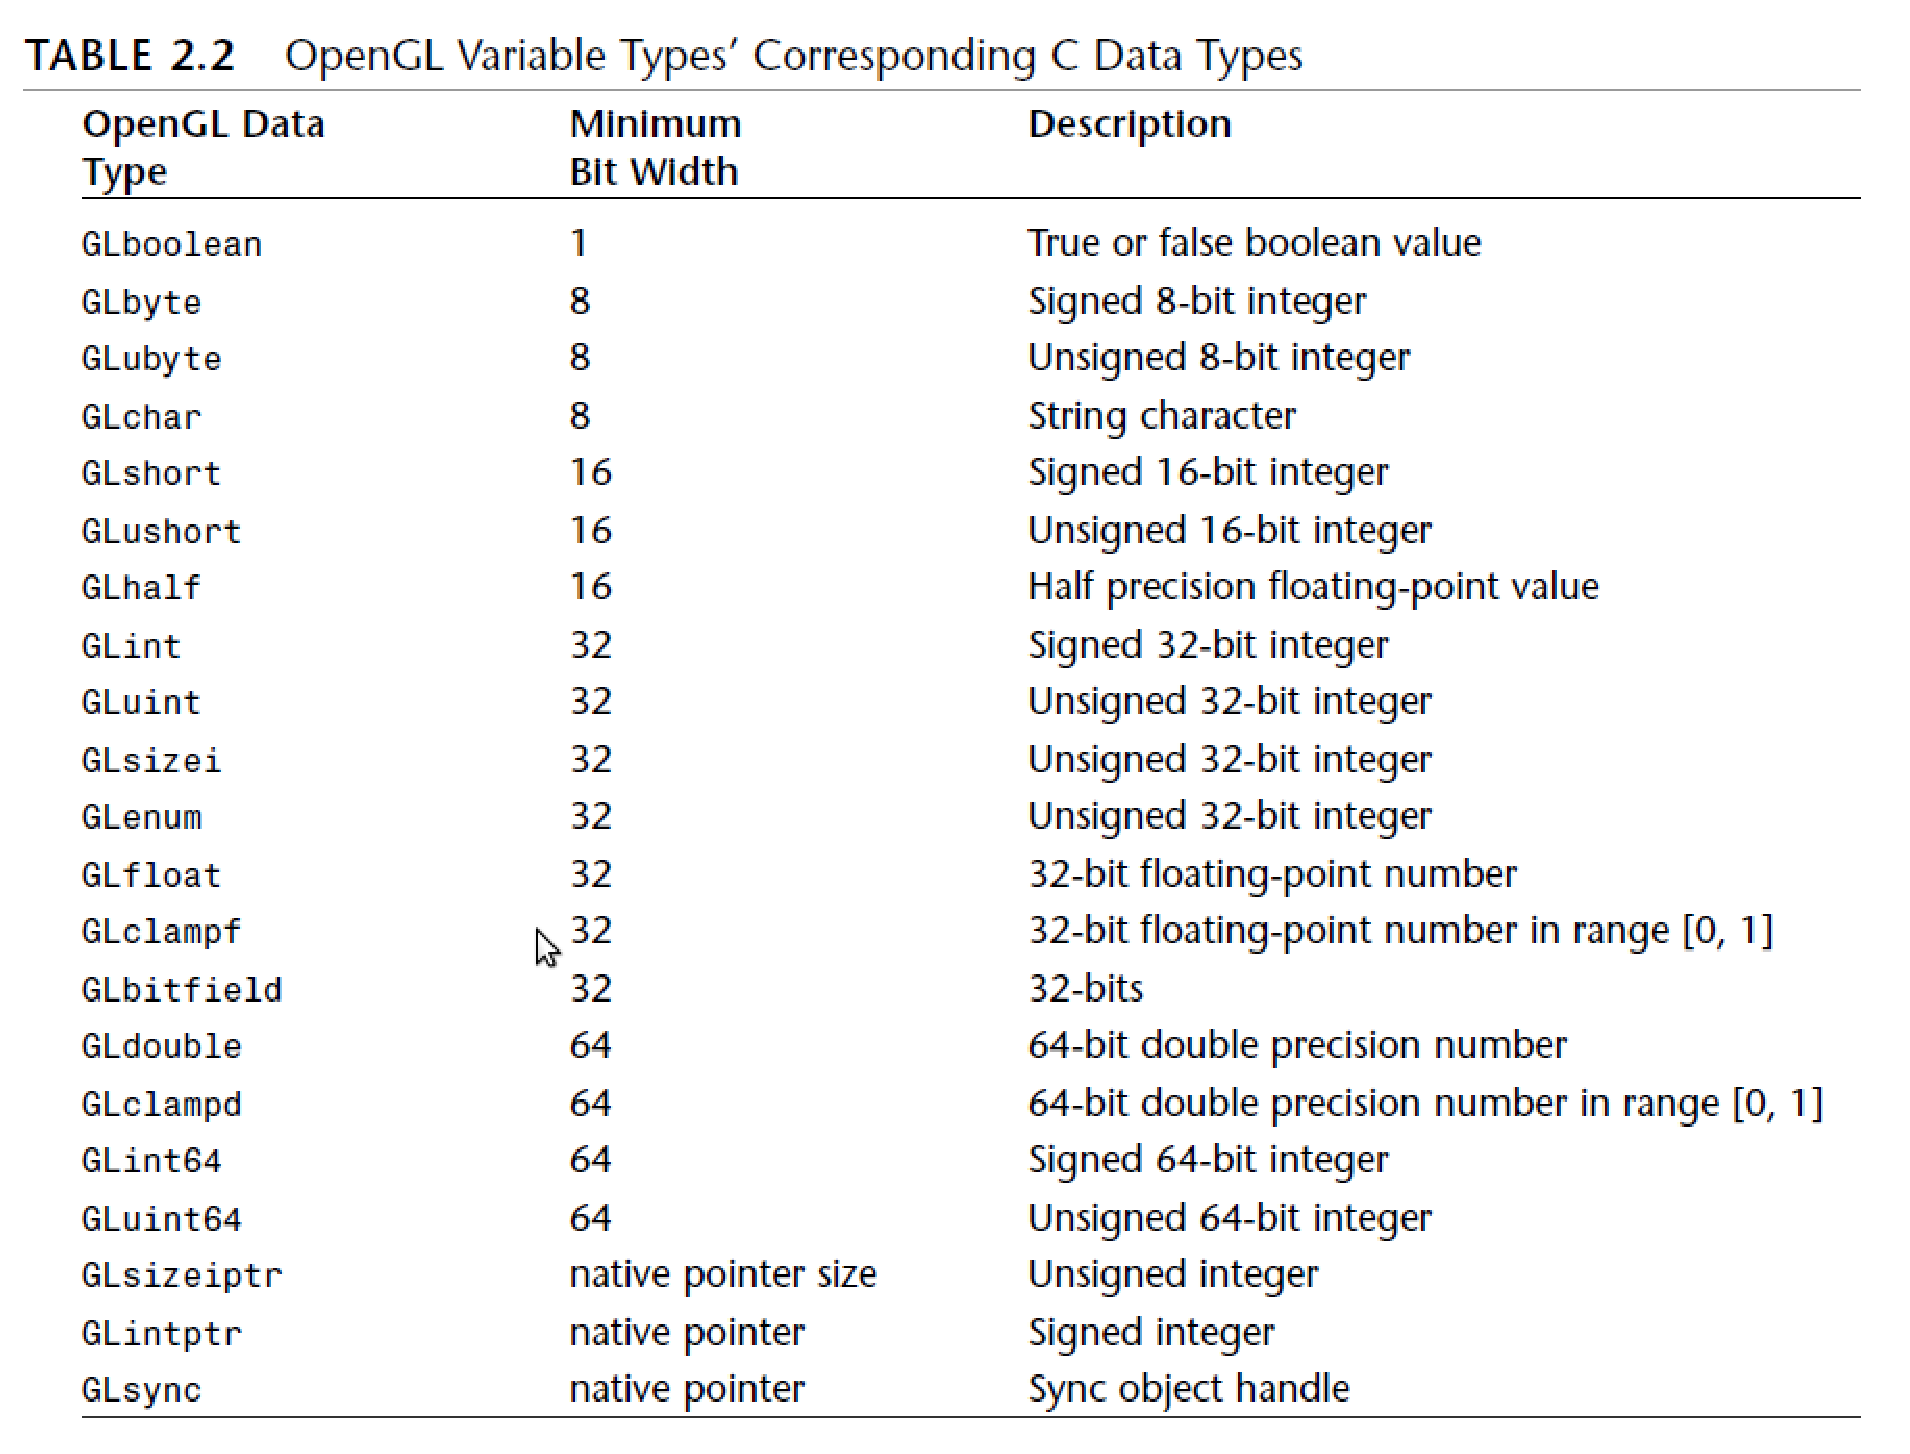
\includegraphics[height=10cm,
    angle=0]{./images/OpenGL_types.eps}}
  \caption{Basic types}
  \label{fig:types}
\end{figure}

The packed formats listed in Table \ref{tab:pixel_data_type} were
introduced in OpenGL 1.2 (and later) as a means of allowing image data
to be stored in a more compressed form that matched a range of color
graphics hardware. These are known as {\bf packed pixel format}. The
number of bits per color channels are shown in the constants

\begin{table}[hbt]
  \begin{center}
    \caption{Data Types for Pixel Data}
    \begin{tabular}{lp{6cm}} 
      \hline
      Constant & Description \\
      \verb!GL_UNSIGNED_BYTE! & Each color component is an 8-bit unsigned
      integer. \\
      \verb!GL_BYTE! & Signed 8-bit integer. \\
      \verb!GL_UNSIGNED_SHORT! & Unsigned 16-bit integer. \\
      \verb!GL_SHORT! & Signed 16-bit integer. \\
      \verb!GL_UNSIGNED_INT!& Unsigned 32-bit integer.\\
      \verb!GL_INT! & Signed 32-bit integer.\\
      \verb!GL_FLOAT!& Single-precision float.\\
      \verb!GL_HALF_FLOAT! & Half-precision float. \\
      \verb!GL_UNSIGNED_BYTE_3_2_2! & Packed RGB values.\\
      \verb!GL_UNSIGNED_BYTE_2_3_3_REV! & Packed RGB values.\\
      \verb!GL_UNSIGNED_SHORT_5_6_5! &Packed RGB values. \\
      \verb!GL_UNSIGNED_SHORT_5_6_5_REV!& Packed RGB values.\\
      \verb!GL_UNSIGNED_SHORT_4_4_4_4! &Packed RGBA values. \\
      \verb!GL_UNSIGNED_SHORT_4_4_4_4_REV!& Packed RGBA values. \\
      \verb!GL_UNSIGNED_SHORT_5_5_5_1!& Packed RGBA values.\\
      \verb!GL_UNSIGNED_SHORT_1_5_5_5_REV! & Packed RGBA values. \\
      \verb!GL_UNSIGNED_INT_8_8_8_8! & Packed RGBA values.\\
      \verb!GL_UNSIGNED_INT_8_8_8_8_REV! & Packed RGBA values. \\
      \verb!GL_UNSIGNED_INT_10_10_10_2! & Packed RGBA values.\\
      \verb!GL_UNSIGNED_INT_2_10_10_10_REV! & Packed RGBA values. \\
      \verb!GL_UNSIGNED_INT_24_8! & Packed RGBA values.\\
      \verb!GL_UNSIGNED_INT_10F_11F_11F_REV! & Packed RGBA values. \\
      \verb!GL_FLOAT_32_UNSIGNED_INT_24_8_REV! & Packed RGBA values \\
      \hline\hline
    \end{tabular}
  \end{center}
  \label{tab:pixel_data_type}
\end{table}


\section{Colors}
\label{sec:colors}

Fig.~\ref{fig:common_colors}

\begin{figure}[hbt]
  \centerline{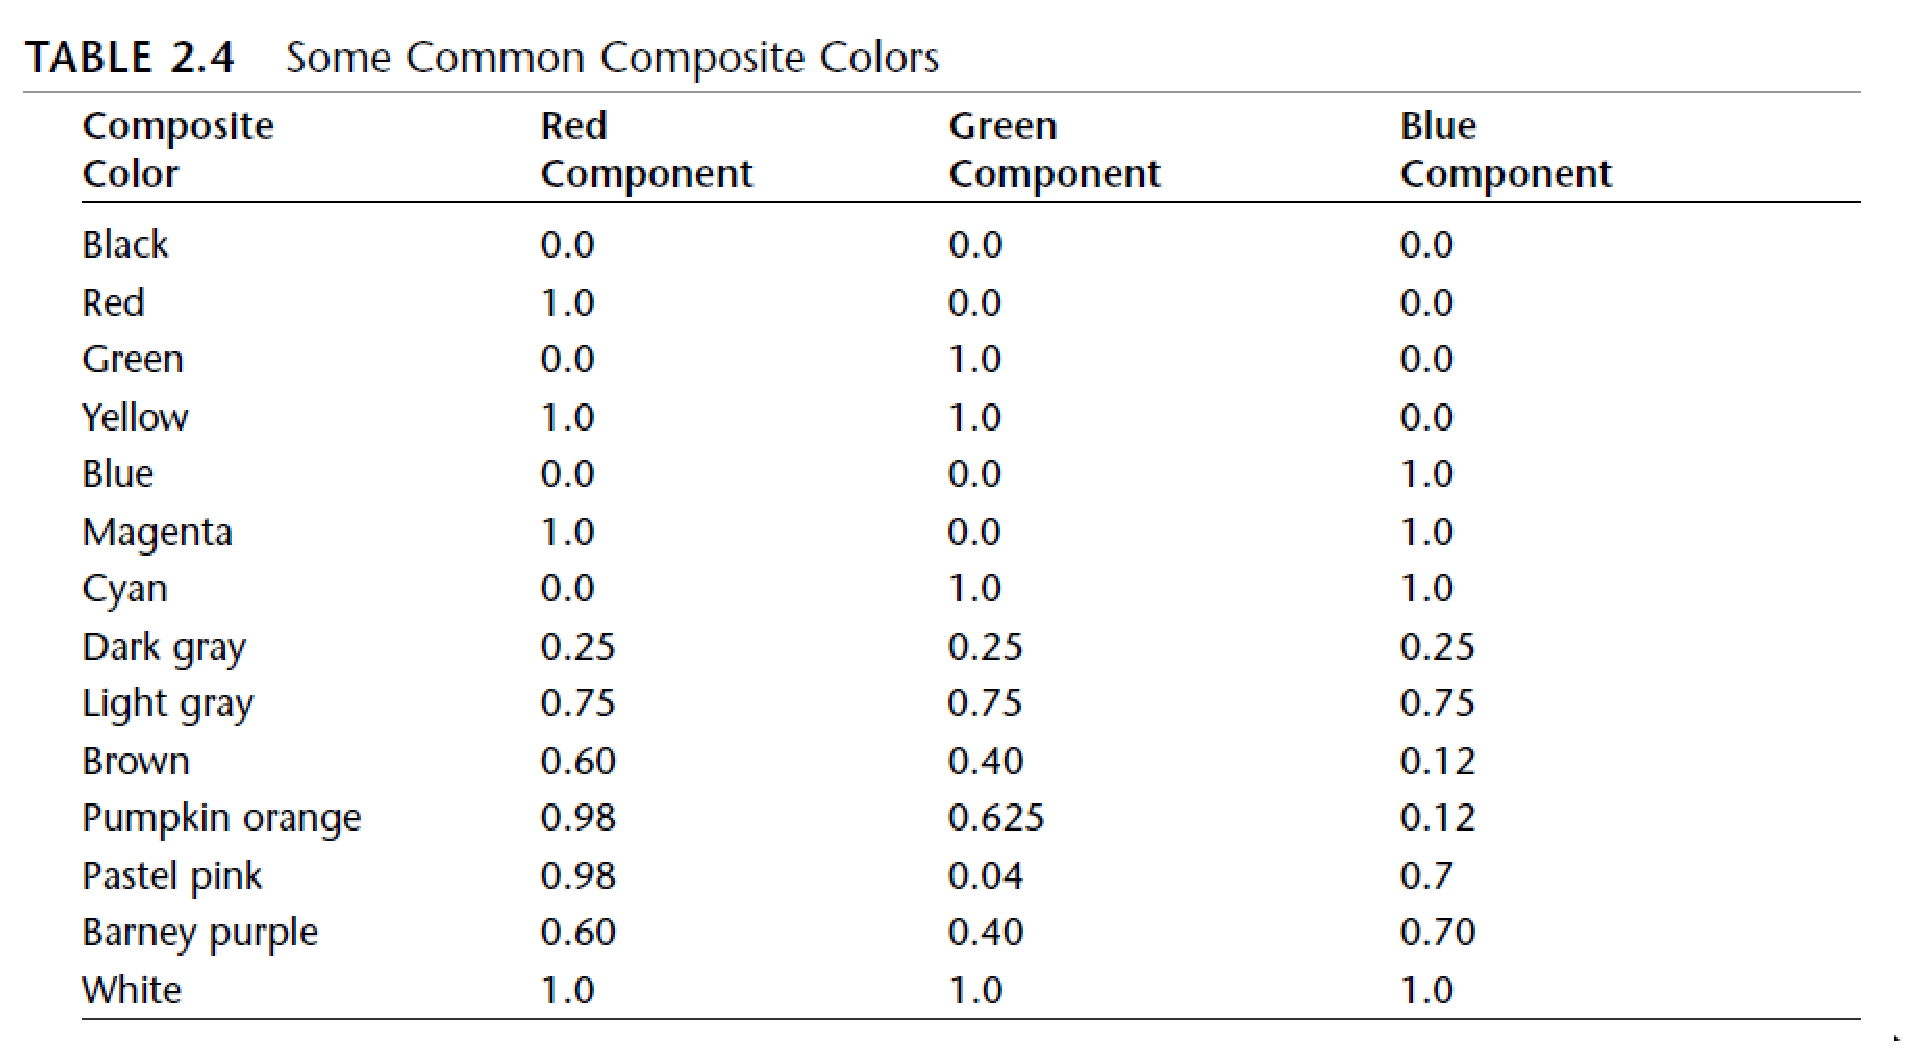
\includegraphics[height=8cm,
    angle=0]{./images/common_colors.eps}}
\caption{Common colors in OpenGL}
\label{fig:common_colors}
\end{figure}

Table~\ref{tab:OpenGL_color} in which the last three format
\begin{verbatim}
GL_STENCIL_INDEX, GL_DEPTH_COMPONENT, and GL_DEPTH_STENCIL
\end{verbatim}
are used for reading and writing directly to the stencil and depth
buffers.

\begin{table}[hbt]
  \begin{center}
    \caption{OpenGL pixel formats}
    \begin{tabular}{cp{9cm}} 
      \hline
      Constant & Description \\
      \verb!GL_RGB! & Colors are in red, green, blue order. \\
      \verb!GL_RGBA! & Colors are in red, green, blue, alpha order.\\
      \verb!GL_BGR!& Colors are in blue, green, red order.\\
      \verb!GL_BGRA!& Colors are in blue, green, red, alpha order.\\
      \verb!GL_RED!& Each pixel contains a single red component.\\
      \verb!GL_GREEN!& Each pixel contains a single green component.\\
      \verb!GL_BLUE!& Each pixel contains a single blue component.\\
      \verb!GL_RG!& Each pixel contains a red followed by a blue component.\\
      \verb!GL_RED_INTEGER!& Each pixel contains a red integer component.\\
      \verb!GL_GREEN_INTEGER!& Each pixel contains a green integer component.\\
      \verb!GL_BLUE_INTETER!& Each pixel contains a blue integer component.\\
      \verb!GL_RG_INTEGER!& Each pixel contains a red followed by a green integer component.\\
      \verb!GL_RGB_INTEGER!& Each pixel contains a red, green, and blue integer component, in
      that order.\\
      \verb!GL_RGBA_INTEGER! & Each pixel contains a red, green, blue, and alpha integer component,
      in that order.\\
      \verb!GL_BGR_INTEGER!& Each pixel contains a blue, green, and red integer component, in
      that order.\\
      \verb!GL_BGRA_INTEGER!& Each pixel contains a blue, green, red, and alpha integer component,
      in that order.\\
      \verb!GL_STENCIL_INDEX!& Each pixel contains a single stencil value.\\
      \verb!GL_DEPTH_COMPONENT!& Each pixel contains a single depth value.\\
      \verb!GL_DEPTH_STENCIL!& Each pixel contains a depth and a stencil value.\\
      \hline\hline
    \end{tabular}
  \end{center}
  \label{tab:OpenGL_color}
\end{table}


\section{Geometric Primitives}
\label{sec:primitives}

Given the vertices defined (Sect.~\ref{sec:attributes}), you now can
connect them to form complex geometric shapes. OpenGL has helped you
creating some basic shapes called primitives.

There are 10 primitives in OpenGL,
Table~\ref{tab:geometric_primitives}.

\begin{table}[hbt]
  \begin{center}
    \caption{OpenGL primitives\protect\footnotemark[1]}
    \footnotetext[1]{We now have: GL\_QUADS, GL\_QUAD\_STRIP,
      GL\_POLYGON}
    \begin{tabular}{cp{8cm}} 
      \hline
      Primitive &  Description\\
      \verb!GL_POINTS! & Each vertex is a single point on the screen. \\
      \verb!GL_LINES! &  Each pair of vertices defines a line segment. \\
      \verb!GL_LINE_STRIP! & A line segment is drawn from the first vertex to each successive vertex.\\
      \verb!GL_LINE_LOOP! & Same as \verb!GL_LINE_STRIP!, but the last and first
      vertex are connected. \\
      \verb!GL_TRIANGLES! & Every three vertices define a new triangle. \\
      \verb!GL_TRIANGLE_STRIP! & Triangles share vertices along a strip. \\
      \verb!GL_TRIANGLE_FAN! & Triangles fan out from an origin, sharing adjacent
      vertices.\\
      \hline\hline
    \end{tabular}
  \end{center}
  \label{tab:geometric_primitives}
\end{table}

% Besides using \verb!GL_POINTS!,
% i.e. each data element is a point, we can also use
% \begin{verbatim}
% GL_LINES, GL_LINE_STRIP, GL_LINE_LOOP,
% GL_TRIANGLES, GL_TRIANGLES_STRIP, GL_TRIANGLES_FAN,
% \end{verbatim}

\subsection{Points}
\label{sec:points}

By default, a point is just a single pixel on the screen. However, you
can change the point size
\begin{verbatim}
void glPointSize(GLfloat size);
\end{verbatim}
or
\begin{verbatim}
// enable the mode
glEnable(GL_PROGRAM_POINT_SIZE);

// and use shader built-in variable
gl_PointSize = 5.0; 
\end{verbatim}

As not all point sizes are supported, you use this to query
\begin{verbatim}
GLfloat sizes[2]; // Store supported point size range
GLfloat step; // Store supported point size increments

  // Get supported point size range and step size
glGetFloatv(GL_POINT_SIZE_RANGE,sizes);
glGetFloatv(GL_POINT_SIZE_GRANULARITY,&step);
\end{verbatim}

\begin{framed}
  The OpenGL specification requires only that one point size, 1.0, be
  supported, but most implementations support a wide range of point
  sizes.
\end{framed}

\subsection{Lines}
\label{sec:lines}

A batch of lines should consist of an even number of vertices.

Lines, by default, are one pixel in width. You can change using
\begin{verbatim}
void glLineWidth(GLfloat width);
\end{verbatim}

\subsection{Line strip}
\label{sec:line-strip}

\subsection{Line loop}
\label{sec:line-loop}

\subsection{Triangles}
\label{sec:triangles}

With 3 vertices, there are different ways of combination of order and
direction in which the vertices are specified to form the same
triangle. Each of combination is called {\bf winding}. The triangles
in Fig.~\ref{fig:winding} are said to have clockwise winding because they are
literally wound in the clockwise direction.

\begin{figure}[hbt]
  \centerline{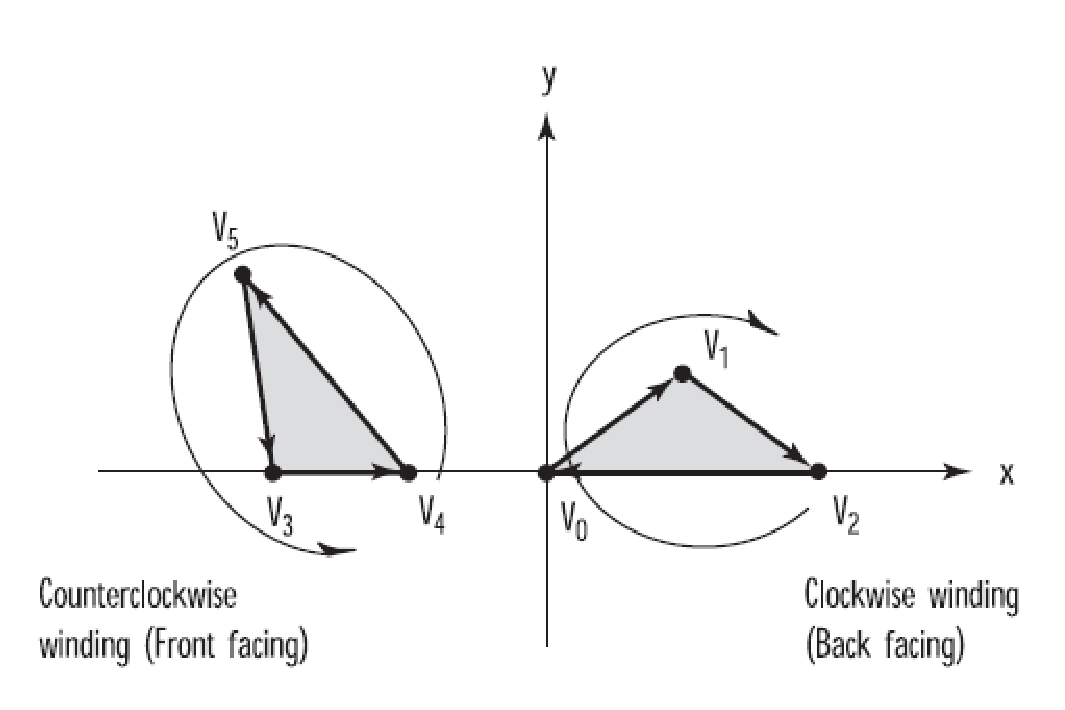
\includegraphics[height=5cm,
    angle=0]{./images/winding.eps}}
  \caption{Winding}
  \label{fig:winding}
\end{figure}

A 2D primitive, like a triangle, has 2 faces.  OpenGL, by default,
considers polygons that have counterclockwise winding to be front
facing. You can change, but make sure use the same convention for all
geometric shapes in your picture.
\begin{verbatim}
glFrontFace(GL_CW);   // or GL_CCW
\end{verbatim}

\begin{figure}[hbt]
  \centerline{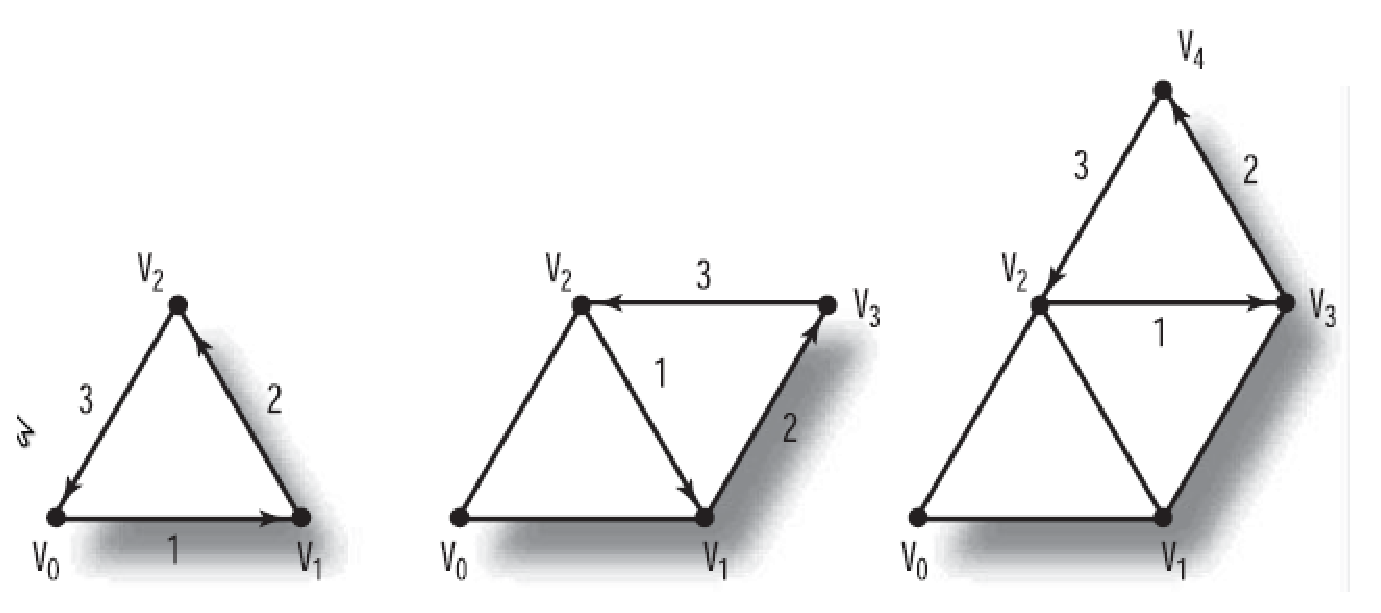
\includegraphics[height=5cm,
    angle=0]{./images/triangle_strip.eps}}
  \centerline{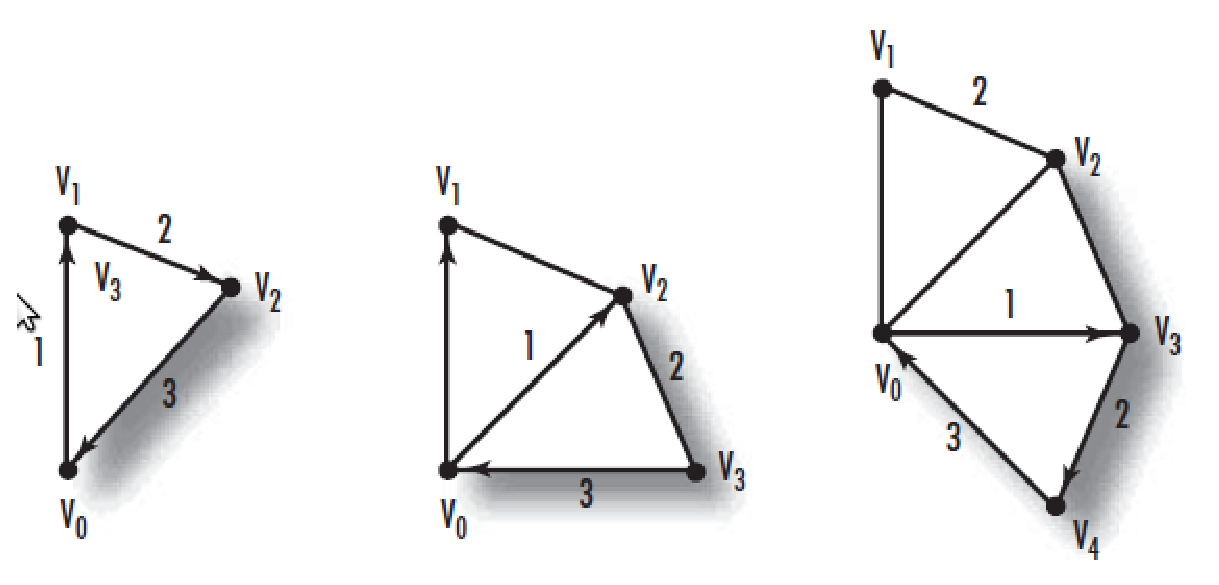
\includegraphics[height=5cm,
    angle=0]{./images/triangle_fan.eps}}

  \caption{(A) triangle strip, (B) triangle fan}
  \label{fig:triangle}
\end{figure}






\chapter{OpenGL applications}
\label{chap:OpenGL_app}

%\lstloadlanguages{[Visual]C++,[ISO]C++}
\lstset{language={[ISO]C++}}
\lstset{numbers=left, numberstyle=\tiny,
  stepnumber = 5, numbersep=5pt, keywordstyle=\color{blue}}

With OpenGL, you must build up your desired model from a small set of geometric
primitives (Sect.\ref{sec:primitives}) - points, lines, and polygons.
A sophisticated library that provides these features could certainly be built on top of OpenGL.
\begin{itemize}
  \item GLU - Sect.\ref{sec:glu}. GLU is a standard part of every OpenGL
  implementation
  
  \item Open Inventor: available separately for many implementations of OpenGL
\end{itemize}

OpenGL is a state machine (Sect.\ref{sec:state-mach-glen}).

Naive draw loop
\begin{lstlisting}
foreach (object) 
{
   // bind framebuffer
   
   // set depth, blending, etc. states
   
   // bind shaders
   
   // bind textures
    
   // bind vertex/index buffers
   
   WriteUniformData (object);
   glDrawElement(
       GL_TRIANGLES,
       object->indexCount,
       GL_UNSIGNED_SHORT,
       0);

}
\end{lstlisting}



\section{Client/Server}
\label{sec:clientserver}

In OpenGL's case, the client side is code that lives in the main CPU's
memory and is executed within the application program, or within the
driver in main system memory.  The rendering commands and data and
sends to the server for execution.
\begin{figure}[hbt]
  \centerline{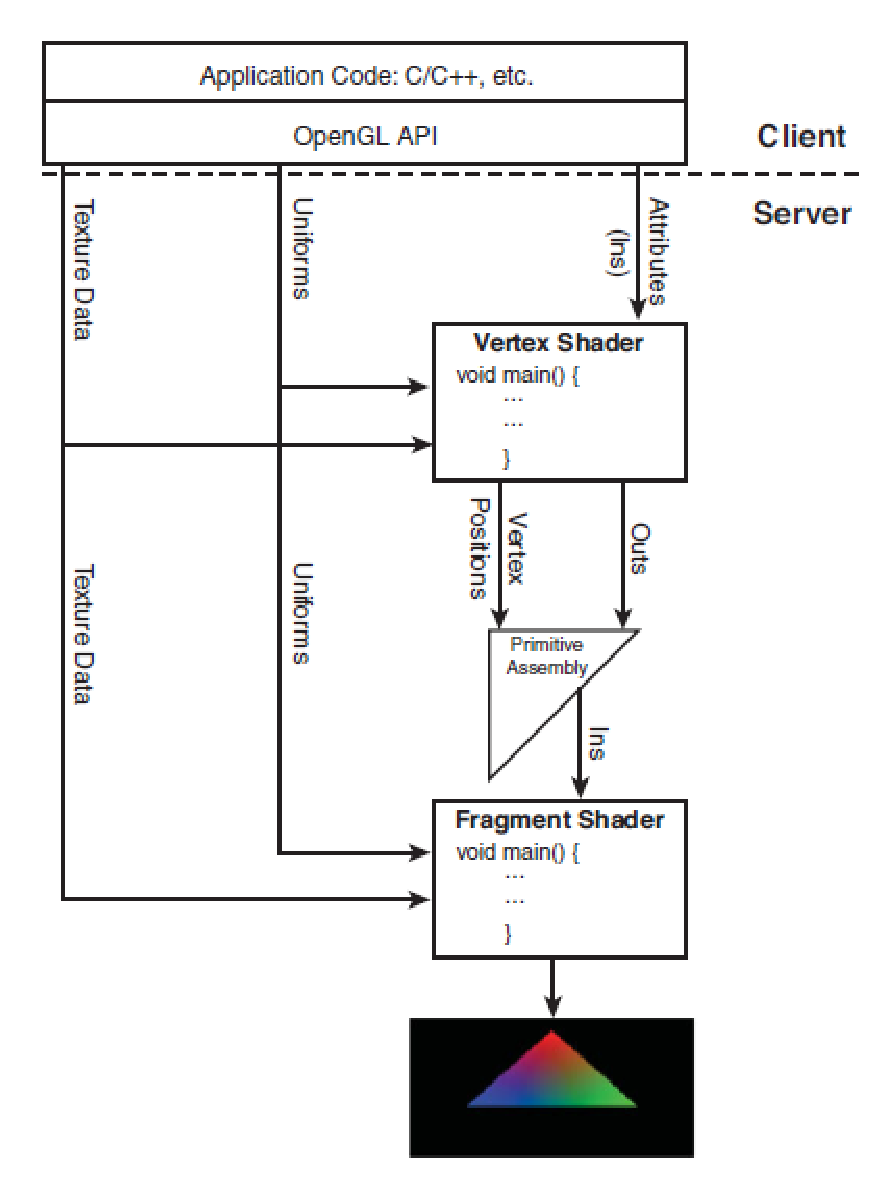
\includegraphics[height=8cm,
    angle=0]{./images/client_server.eps}}
  \caption{Steps to render a triangle}
  \label{fig:client_server}
\end{figure}

{\bf Shaders} are programs (with its own main() function) running on
server sides. There are two types: vertex shaders and fragment
shaders, Fig.~\ref{fig:client_server}. Both are written by the
language
GLSL\footnote{In general, we may have geometry shader that can
  (optionally) fit between, as well as sort of feedback mechanism for
  moving data back and forth. There can be also some post fragment
  processing features such as blending, stencil, and depth testing}.
Nowadays, we can programs shaders programs, using CUDA - a C
extension, under the name {\bf kernels} in CUDA context. We can easily
map the data from CUDA memory space to OpenGL memory space easily via
Map/Unmap mechanism (read Sect.~\ref{sec:cuda-app.-with}).

A vertex shader do the job for a single vertex (data incoming from the
client), including: applying transformations, or doing other types of
math to calculate lighting effects, displacement, color values, and so
on. To render a triangle with three vertices, the vertex shader is
executed three times, once for each vertex.

Data passed to shaders are called attributes and are composed of
\begin{enumerate}
\item vertex (location information)

\item color

\item normal (surface normal)

\item uniforms, 

\item textures.(primary + secondary)
\end{enumerate}


\subsection{Attributes (vertex, color)}
\label{sec:attributes}

An attribute is something that change per vertex. So, they can be
\begin{enumerate}
\item location (maximum 3 components) - XYZ
\item color (maximum 4 components) - RGBA
\end{enumerate}
Attributes can be floating-point, integer, or boolean data, and
attributes are always stored internally as a four component vector,
even if you don't use all four components.

% Attributes, however, can have any meaning you want in the vertex
% program; you are in control.


\begin{framed}
  Attributes are copied from a pointer to local client memory to a
  buffer that is stored (most likely) on the graphics
  hardware. Attributes are only processed by the vertex shader (read
  Sect.~\ref{sec:shaders}) and have no meaning to the fragment shader.
\end{framed}

Everything starts with the atoms ``vertex''. Each vertex can have some
attributes (maximum 16, numbered from 0 to 15 and can be assigned to
any variable in the shader program). 

\begin{table}[hbt]
  \begin{center}
    \caption{Predefined attribute identifiers}
    \begin{tabular}{cp{8cm}} 
      \hline
      Identifier & Description \\
      \verb!GLT_ATTRIBUTE_VERTEX! & Three component (x, y, z) vertex position\\
      \verb!GLT_ATTRIBUTE_COLOR! & Four component (r, g, b, a) color value\\
      \verb!GLT_ATTRIBUTE_NORMAL! & Three components (x, y, z) surface
      normal \\
      \verb!GLT_ATTRIBUTE_TEXTURE0! & Primary two component (s, t) texture
      coordinate \\
      \verb!GLT_ATTRIBUTE_TEXTURE1! & Secondary two component (s, t) texture
      coordinate \\
      \hline\hline
    \end{tabular}
  \end{center}
  \label{tab:attribute_id}
\end{table}

% \begin{verbatim}
% GLT_ATTRIBUTE_VERTEX
% GLT_ATTRIBUTE_COLOR 
% GLT_ATTRIBUTE_NORMAL 
% GLT_ATTRIBUTE_TEXTURE0
% GLT_ATTRIBUTE_TEXTURE1 
% \end{verbatim}

\subsection{Uniforms}
\label{sec:uniforms}

A uniform is a single value that doesn't change for the entire batch
attributes. Uniforms can be used for virtually an unlimited number of
uses.

\begin{itemize}
\item set a single color value that is applied to an entire surface. 
\item set a time value that you change every time you render to do
  some type of vertex animation (note the uniform changes once per
  batch, not once per vertex here).

\item One of the most common uses of uniforms is to set transformation
  matrices in the vertex shader (this is almost the entire purpose
\end{itemize}
Like attributes, uniform values can be floating-point, integer, or
boolean in nature, but unlike attributes, you can have uniform
variables in both the vertex and the fragment shader.

\begin{framed}
  Uniforms can be scalar or vector types, and you can have matrix uniforms.
\end{framed}


\subsection{Textures}
\label{sec:textures}

Texture values can be sampled and filtered from both the vertex shader
and the fragment shader.  Fragment shaders typically sample a texture
to apply image data across the surface of a triangle.

Texture data, however, is more useful than just to represent
images. Most image file formats store color components in unsigned
byte values (8 bits per color channel), but you can also have
floating-point textures. This means potentially any large block of
floating- point data, such as a large lookup table of an expensive
function, could be passed to a shader in this way.

We will learn more in Sect.~\ref{sec:arrays-=-textures}. 
% \section{Vertex}
% \label{sec:vertex}



\section{State machine (glEnable/glDisable)}
\label{sec:state-mach-glen}

You put it into various states (or modes) that then remain in effect until you
change them. As you've already seen, the current color is a state variable. 

For a given piece of geometry, there are many things that can affect
how it is drawn, e.g. 
\begin{itemize}
\item is the object blended in the background?
\item are we performing front or back face culling?
\item ...
\end{itemize}
The collection of all of these parameters is called a {\bf state} of
the pipeline. So, OpenGL works as a state machine. The state variables
in general can have more than 2 values.

\url{http://www.glprogramming.com/red/chapter01.html}

For those that receives one of two possible values only, they are
associated with turn on or off. So, OpenGL provides 2 functions to do
this: \verb!glEnable/glDisable!.
\begin{verbatim}
void glEnable(GLenum capability);

void glDisable(GLenum capability);

GLboolean glIsEnabled(GLenum capability);
\end{verbatim}


E.g.: depth testing if enabled, will force OpenGL to check to make
sure the object is in front of other things behind it, before being
rendered. 
\begin{verbatim}
glEnable(GL_DEPTH_TEST);
\end{verbatim}


For those that can receive more than 2 values. A set of query
functions allows you to query the values of Booleans, integers,
floats, and double variables. These four functions are prototyped
thus:
\begin{verbatim}
void glGetBooleanv(GLenum pname, GLboolean *params);
void glGetDoublev(GLenum pname, GLdouble *params);
void glGetFloatv(GLenum pname, GLfloat *params);
void glGetIntegerv(GLenum pname, GLint *params);
\end{verbatim}
Each function returns a single value or a whole array of values,
storing the results at the address you supply.



\section{Intermediate mode vs. Vertex Arrays vs. Display List}
\label{sec:interm-mode-vs}

This section describes different programming approaches used in
OpenGL. 

\subsection{Intermediate mode}
\label{sec:intermediate-mode-1}

{\bf Intermediate-Mode is the firs approach}, used in OpenGL 1.0. In
this mode, all rendering functions are called between
\verb!glBegin/glEnd!. So, it requires explicit functional calls to
draw every geometric primitive shapes. They can be

\begin{enumerate}
\item \verb!glVertex[size][type]v! : call this OpenGL API to specify
  the location of the vertex (2D or 3D ...)

  with \verb!size! is 2, 3 or 4; \verb!type! is any of [s,i,f,d]
  (corresponding to short, int, float, and double). 

\item For other types of arrays, we have similar syntax,
  e.g. \verb!glColor[size][type]v!, \verb!glNormal[size][type]v!...
\end{enumerate}

However, this approach would be come slow for complex geometric
primitive composed of thousands of vertex due to thousands of
functional calls and many of them are redundant. Another factor that
slow down the performance is that data need to be transferred so often
from CPU RAM to GPU RAM. 

\subsection{Vertex Arrays}
\label{sec:vertex-arrays}

To resolve the first problem, i.e. functional call redundancy, OpenGL
1.1 introduced vertex data into arrays, and then use blocks of data in
these arrays to specify the multiple geometric primitives through the
execution of a single command.
\begin{verbatim}
  // Setup a triangle
  // Here, we use vertex array, i.e. every triple form a vertex
  GLfloat vVerts[] = { -0.5f, 0.0f, 0.0f,
                    0.5f, 0.0f, 0.0f,
                    0.0f, 0.5f, 0.0f };
\end{verbatim}
which we use to 
\begin{verbatim}
  // create a Vertex Array object
  glGenBuffers(1, &uiVertexArray);
  // bind to ARRAY BUFFER
  glBindBuffer(GL_ARRAY_BUFFER, uiVertexArray);
  // finally, add data to it
  glBufferData(GL_ARRAY_BUFFER, sizeof(GLfloat) * 3 * nNumVerts, 
               vVerts, GL_DYNAMIC_DRAW);
\end{verbatim}
In complicated case, we can check
\begin{verbatim}
  // First time, create the buffer object, allocate the space
  if(uiVertexArray == 0) {
        glGenBuffers(1, &uiVertexArray);
        glBindBuffer(GL_ARRAY_BUFFER, uiVertexArray);
        glBufferData(GL_ARRAY_BUFFER, 
              sizeof(GLfloat) * 3 * nNumVerts, 
              vVerts, GL_DYNAMIC_DRAW);
        }
  else        { // Just bind to existing object
        glBindBuffer(GL_ARRAY_BUFFER, uiVertexArray);

        // Copy the data in
        glBufferSubData(GL_ARRAY_BUFFER, 0, 
                  sizeof(GLfloat) * 3 * nNumVerts, vVerts);
        pVerts = NULL;
        }
  }
\end{verbatim}

\textcolor{red}{We can use up to 6 arrays: corresponding to arrays of
  vertices, normals, colors components, color indices, texture
  coordinates, Boolean edge flags}.
We use the following 6 functions to specify the location, and data
format of the corresponding type of
array\footnote{\url{http://personal.redestb.es/jmovill/opengl/openglonwin-15.html}}.

\begin{verbatim}
glVertexPointer(int size, enum type, sizei stride, void *pointer)
glNormalPointer(...)
glColorPointer
glIndexPointer
glTexCoordPointer
glEdgeFlagPointer
\end{verbatim}
with (suppose Vertex Array)
\begin{enumerate}
\item \verb!size! = number of coordinates per vertex (e.g. with 3D
  vertex, size = 3)
\item \verb!type! = data type for each coordinate
  (\verb!GL_SHORT, GL_INT!, \verb!GL_FLOAT, or GL_DOUBLE!)

  Other array types may use different data type, e.g. Boolean edge
  flags only use \verb!GL_BOOL!
\begin{verbatim}
glVertexPointer   2,3,4   short, int, float, double
glNormalPointer   3       byte, short, int, float, double
glColorPointer 	  3,4     byte, ubyte, short, ushort, int,  
                          uint, float, double 
glIndexPointer    1       ubyte, short, int, float, double
glTexCoordPointer 1,2,3,4 short, int, float, double
glEdgeFlagPointer 1       boolean
\end{verbatim}

\item \verb!stride! = byte offset between pointers to consecutive
  vertexes (if stride = 0, the vertex data are tightly packed)
\item \verb!pointer! = the pointer pointing to the first coordinate of
  the first vertex in the array. 
\end{enumerate}

\begin{framed}
  Data components within an array element are stored
  sequentially. Array elements can be non-contiguous, i.e. when stride
  $.ne.$ 0. If stride = 0, then array elements are stored sequentially
  as well. 
\end{framed}

% gl[...]Pointer: OpenGL give 6 different pointers when using
% glDrawArrays/Elements. The most commonly use function is
% \verb!glVertexPointer()!.

These data reside on client-side, and are disabled by default. So, we
need to enable which one we want to use using
\verb!glEnableClientState(enum array)! and
\verb!glDisableClientState(..)!  with \verb!array! token can be.
\begin{verbatim}
GL_VERTEX_ARRAY
GL_NORMAL_ARRAY
GL_COLOR_ARRAY
GL_INDEX_ARRAY
GL_TEXTURE_COORD_ARRAY
GL_EDGE_FLAG_ARRAY
\end{verbatim}

\begin{framed}
  We generally discuss Vertex Array, as other type of arrays mainly
  provide accompanying information to the Vertex Array and most of the
  time we work with Vertex Array data.

  \textcolor{red}{Like intermediate-mode, the data in Vertex Arrays
    reside in CPU RAM, and need to move to server-side memory (i.e. GPU
    DRAM) every time rendering is required}.
\end{framed}


To render data using Vertex Arrays, new OpenGL APIs are provided and
used between \verb!glBegin/glEnd!

\begin{enumerate}
\item \verb!glArrayElement(int i )!: transfer (i.e. draw) the element
  $i$-th to OpenGL (i.e. GPU memory), i.e. draw points from a single
  array.

\item \verb!glDrawArrays!: (combine array elements from different
  enabled arrays) for each enabled array, we construct a sequence of
  geometric primitives using array elements from \verb!first! through
  \verb!count! of each enabled array.
\begin{verbatim}
void glDrawArrays ( enum mode, int first, sizei count ) ;
\end{verbatim}
  with \verb!mode! tell which kind of primitive to construct (the same
  token passing to \verb!glBegin()!. 

  So, we don't need to work with individual vertexes, OpenGL will
  automatically iterate through array elements and do the work

\item \verb!glDrawElements()!: (combine continuous array elements from
  a single array) we iterate through array elements in the array
  specified by \verb!indices! and call \verb!glArrayElement()! for
  each element until it reaches \verb!count! element count.
\begin{verbatim}
void glDrawElements ( enum mode, sizei count, 
                 enum type, void *indices );
\end{verbatim}
  with \verb!mode!, again, is the type of geometric primitive to
  construct. 

\item \verb!glInterleavedArrays!: (combine interleaved elements from a
  single array) allow sending vertices data to the graphics card using
  a single array
\begin{verbatim}
void glInterleavedArrays ( enum format, sizei stride, void *pointer )
\end{verbatim}

\item If any of the arrays other Vertex Arrays are enabled, they are
  indeterminate after the execution of glDrawElements(), otherwise,
  the values are unchanged. 
\end{enumerate}

As a result, with the OpenGL 1.1 (array-based) approach, you would
transfer your few hundred KB of vertex data across the bus every time
you wanted to render a model. This meant that you could modify your
array-based data in memory as the next time you sent it the new data
would be transferred. Compared to (static) display lists, this made
array-based data the natural choice for frequently updated geometry.


Summary of new functions in OpenGL 1.1.
\begin{verbatim}
glArrayElement(), glDrawArrays(), glVertexPointer(), 
glNormalPointer(), glColorPointer(), glIndexPointer(), 
glTexCoordPointer(), glEdgeFlagPointer(), glGetPointerv(), 
glDrawElements(), glInterleavedArrays().
\end{verbatim}

An example is given in Sect.~\ref{sec:example-fortr-freegl-1}. 

\subsection{Display List}
\label{sec:display-list}


{\bf Display List} is a list of OpenGL commands that are executed only
once and the result are stored on the server side, i.e. GPU. After the
display list has been compiled and executed, we can reuse the result
as many time as we want without re-evaluating nor re-transmitting from
client (CPU) to server (GPU). However, they cannot be modified. So,
this method is best for static data.
\textcolor{red}{If we want the data to reside on graphics card memory
  and the data, however, change quite often, it's better to consider
  VBO}.

Data in display list can also be shared by many clients.Since display
list is a part of server state, any client commands cannot be used.
\begin{verbatim}
glFlush(), glFinish(), glRenderMode(), 
glEnableClientState(), glVertexPointer(), etc. 
\end{verbatim}
The same to OpenGL commands that return a value, as the value is
returned to the client side.
\begin{verbatim}
glIsEnabled(), glGet*(), glReadPixels(), 
glFeedbackBuffer(), etc.
\end{verbatim}

How to use display list?
\begin{enumerate}
\item \verb!glGenLists(int num)!: (optional) create one or more
  continuous display list objects. Return 0 if errors occur.

\item Commands in the display lists are between \verb!glNewList()! and
  \verb!glEndList()!, prior to rendering. 
\begin{verbatim}
glNewList(dListID, mode)
...
glEndList()
\end{verbatim}
  with \verb!mode! can be \verb!GL_COMPILE! (compile only),
  \verb!GL_COMPILE_AND_EXECUTE! (compile and then render).

\item Now, to invoke one or more display lists, we use
  \verb!glCallList(dListID)! or \verb!glCallLists()! every frame. We
  put this inside the callback.
\end{enumerate}

\begin{verbatim}
// create one display list
GLuint index = glGenLists(1);

// compile the display list, store a triangle in it
glNewList(index, GL_COMPILE);
    glBegin(GL_TRIANGLES);
    glVertex3fv(v0);
    glVertex3fv(v1);
    glVertex3fv(v2);
    glEnd();
glEndList();
...

// draw the display list
glCallList(index);
...

glCallList(index); //call again (data is now stored in 
                   //server-side, very fast)

// delete it if it is not used any more
glDeleteLists(index, 1);
\end{verbatim}

For example, read Sect.~\ref{sec:example-fortran-glut}.

References:
\begin{itemize}
\item \url{http://www.songho.ca/opengl/gl_displaylist.html}
\end{itemize}


\section{Graphics effects}
\label{sec:graphics-effects}

\subsection{Face culling}
\label{sec:face-culling}

By default, every point, line, or triangle you render is rasterized
on-screen and in the order in which you specify when you assemble the
primitive batch. One problem that can occur is if you draw a solid
object made up of many triangles, the triangles drawn first can be
drawn over by triangles drawn afterward. 

The {\it painter algorithm} draw the farther triangles first, and the
nearer later. However, this is inefficient. A better solution is {\bf
  face culling}. 

Culling away the front of solid geometry is also useful in some
circumstances, for example, showing a rendering of the insides of some
figure. When rendering transparent objects (blending is coming up
soon), we often render an object twice, once with transparency on,
culling the front sides, and then again with the back sides turned
off. This layers the object with the back side rendered before the
front side, a requirement for rendering things transparently.

General face culling is turned on/off like this:
\begin{verbatim}
glEnable(GL_CULL_FACE);

glDisable(GL_CULL_FACE);
\end{verbatim}

Note, we did not say whether to cull the front or back of
anything. That is controlled by another function, glCullFace.
\begin{verbatim}
void glCullFace(GLenum mode);
\end{verbatim}
Valid values for the mode parameter are \verb!GL_FRONT!,
\verb!GL_BACK!, or \verb!GL_FRONT_AND_BACK!. To throw away the insides
of opaque (nontransparent) geometry takes two lines of code then.
\begin{verbatim}
glCullFace(GL_BACK);
glEnable(GL_CULL_FACE);
\end{verbatim}
Back face culling can significantly improve performance and corrects
some problems.

\subsection{Depth testing}
\label{sec:depth-testing}

Another technique for hidden surface removal is called depth
testing. The idea is that when a vertex is drawn, it is assigned a
depth value (z value) that denotes its distance from the viewer's
perspective. Next time, when another vertex is drawn at that location,
it's z value will be used to compared with the current pixel. If the
value is higher, it's closer to the viewer, so the old value of the
pixel is overwritten by this new value. 

Using depth testing is recommended
\begin{verbatim}
glutInitDisplayMode(GLUT_DOUBLE | GLUT_RGBA | GLUT_DEPTH);

glEnable(GL_DEPTH_TEST);
\end{verbatim}

\subsection{Polygon modes}
\label{sec:polygon-modes}

By default, any polygon (triangles, quad, ...) are drawn as
solid. However, you can change the setting (e.g. draw wireframe) using
\begin{verbatim}
void glPolygonMode(GLenum face, GLenum mode);
\end{verbatim}
Like in face culling, the face parameter can be 
\begin{verbatim}
GL_FRONT, GL_BACK, or GL_FRONT_AND_BACK.
\end{verbatim}
The mode parameter can be \verb!GL_FILL! (the default),
\verb!GL_LINE!, or \verb!GL_POINT!. 

\subsection{Polygon offsets}
\label{sec:polygon-offsets}

Sometimes, you want two polygon modes, Fig.~\ref{fig:polygon_offset}

\begin{figure}[hbt]
  \centerline{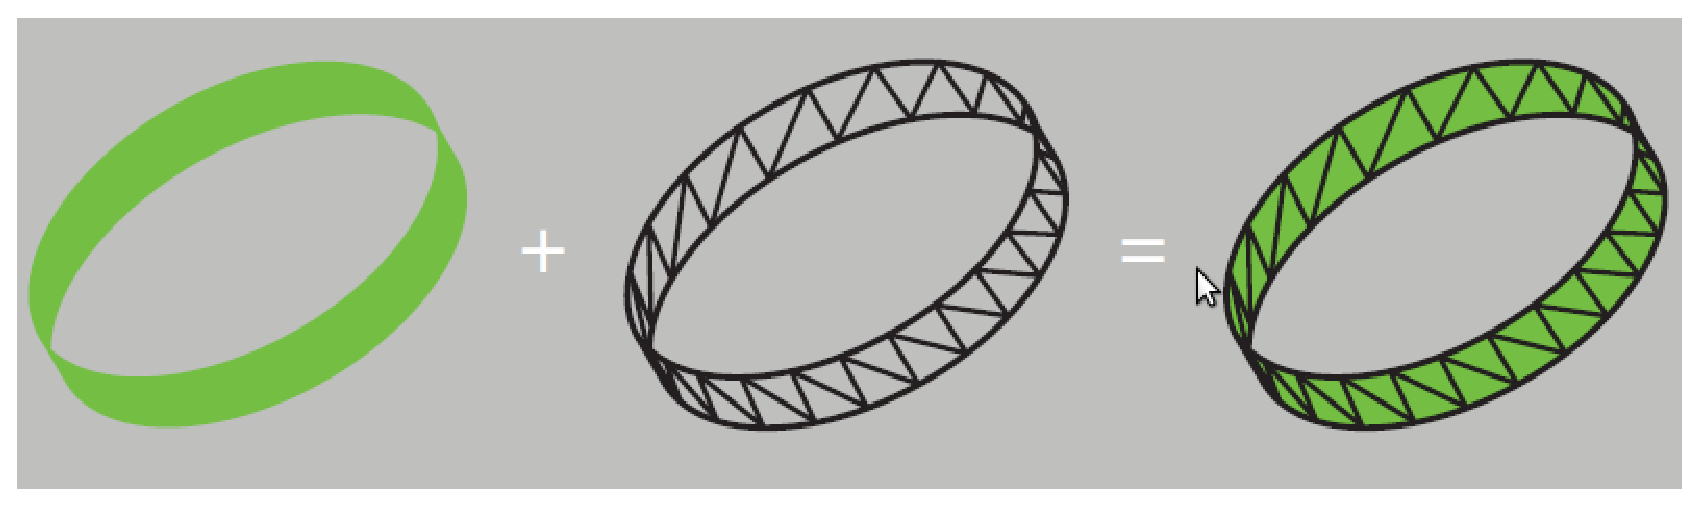
\includegraphics[height=3cm,
    angle=0]{./images/polygon_offset.eps}}
  \caption{When you want both solid and wireframe drawings}
  \label{fig:polygon_offset}
\end{figure}


\subsection{Scissors }
\label{sec:scissors-}

If you know the exact region that need to redrawn, you can explicitly
tell OpenGL to redraw that region only. This can help improve the
performance as the system doesn't have to re-draw all. This is known
as scissor test.

\begin{verbatim}
glEnable(GL_SCISSOR_TEST);

// tell the rectangle
void glScissor(GLint x, GLint y, GLsizei width, GLsizei height);
\end{verbatim}
after that, you can turn off that scissor test.


This is the sample callback
\begin{verbatim}
void RenderScene(void)
{
  // Clear blue window
  glClearColor(0.0f, 0.0f, 1.0f, 0.0f);
  glClear(GL_COLOR_BUFFER_BIT);

// Now set scissor to smaller red sub region
  glClearColor(1.0f, 0.0f, 0.0f, 0.0f);
  glScissor(100, 100, 600, 400);
  glEnable(GL_SCISSOR_TEST);
  glClear(GL_COLOR_BUFFER_BIT);

// Finally, an even smaller green rectangle
glClearColor(0.0f, 1.0f, 0.0f, 0.0f);
glScissor(200, 200, 400, 200);
glClear(GL_COLOR_BUFFER_BIT);

// Turn scissor back off for next render
  glDisable(GL_SCISSOR_TEST);
  
  glutSwapBuffers();
}
\end{verbatim}

\subsection{Blending}
\label{sec:blending}

Blending is a intermediate mode between DEPTH testing ON and OFF. It
means that the color value of the two (or more) vertices at the same
pixel are combined to create the blending effect.

\begin{verbatim}
glEnable(GL_BLEND);
\end{verbatim}

By default, the combined color use the formula (you can change the equation)
\begin{verbatim}
Cf = (Cs * S) + (Cd * D)

Cs  = source color
Cd  = destination color
Cf  = combined color
\end{verbatim}
with S and D are blending factors, given to OpenGl via
\begin{verbatim}
glBlendFunc(GLenum S, GLenum D);
\end{verbatim}
which can be any of the following value,
Table~\ref{tab:blending_factor}. The constant blending factor is
initially black (0.0f, 0.0f, 0.0f, 0.0f), but it can be changed with
this function:
\begin{verbatim}
void glBlendColor(GLclampf red, GLclampf green, 
                  Glclampf blue,
                  GLclampf alpha);
\end{verbatim}

\begin{verbatim}
GLfloat vRed[] = { 1.0f, 0.0f, 0.0f, 0.5f };
glEnable(GL_BLEND);
glBlendFunc(GL_SRC_ALPHA, GL_ONE_MINUS_SRC_ALPHA);
shaderManager.UseStockShader(GLT_SHADER_IDENTITY, vRed);
squareBatch.Draw();
glDisable(GL_BLEND);
\end{verbatim}

\begin{table}[hbt]
  \begin{center}
    \caption{OpenGL blending factor, $f = min(As, 1-Ad)$}
    \begin{tabular}{ccc} 
      \hline
      Function & RGB Blend Factors & Factor \\
      \verb!GL_ZERO! & (0,0,0) &  0 \\
      \verb!GL_ONE!& (1,1,1) & 1 \\
      \verb!GL_SRC_COLOR! & (Rs,Gs,Bs) & As \\
      \verb!GL_ONE_MINUS_SRC_COLOR! & (1,1,1) - (Rs,Gs,Bs) & 1 - As \\
      \verb!GL_DST_COLOR! & (Rd,Gd,Bd) & Ad \\
      \verb!GL_ONE_MINUS_DST_COLOR! & (1,1,1) - (Rd,Gd,Bd) & 1 - Ad \\
      \verb!GL_SRC_ALPHA! & (As,As,As) & As \\
      \verb!GL_ONE_MINUS_SRC_ALPHA! & (1,1,1) - (As,As,As) & 1 - As \\
      \verb!GL_DST_ALPHA! & (Ad,Ad,Ad) & Ad \\
      \verb!GL_ONE_MINUS_DST_ALPHA! & (1,1,1) - (Ad,Ad,Ad) & 1 - Ad  \\
      \verb!GL_CONSTANT_COLOR! & (Rc,Gc,Bc) & Ac \\
      \verb!GL_ONE_MINUS_CONSTANT_COLOR! & (1,1,1) - (Rc,Gc,Bc) & 1 - Ac \\
      \verb!GL_CONSTANT_ALPHA! & (Ac,Ac,Ac) & Ac \\
      \verb!GL_ONE_MINUS_CONSTANT_ALPHA! & (1,1,1) - (Ac,Ac,Ac) & 1 - Ac \\
      \verb!GL_SRC_ALPHA_SATURATE! & (f,f,f)* & 1 \\
      \hline\hline
    \end{tabular}
  \end{center}
  \label{tab:blending_factor}
\end{table}

You can change the equation using
\begin{verbatim}
void glBlendEquation(GLenum mode);
\end{verbatim}
with mode is given in Table~\ref{tab:blending_equation}. Or you can
give your own equation for RGB and another for Alpha channel.
\begin{verbatim}
void glBlendFuncSeparate(GLenum srcRGB, GLenum dstRGB, 
              GLenum srcAlpha, 
              GLenum dstAlpha);
\end{verbatim}


\begin{table}[hbt]
  \begin{center}
    \caption{Blending formula}
    \begin{tabular}{cc} 
      \hline
      Mode & Function \\
      \verb!GL_FUNC_ADD! (default) & Cf = (Cs * S) + (Cd * D) \\
      \verb!GL_FUNC_SUBTRACT! & Cf = (Cs * S) - (Cd * D) \\
      \verb!GL_FUNC_REVERSE_SUBTRACT! & Cf = (Cd * D) - (Cs * S) \\
      \verb!GL_MIN! & Cf = min(Cs, Cd) \\
      \verb!GL_MAX! & Cf = max(Cs, Cd) \\
      \hline\hline
    \end{tabular}
  \end{center}
  \label{tab:blending_equation}
\end{table}

\subsection{Anti-aliasing}
\label{sec:anti-aliasing}

First
\begin{verbatim}
// blend equation is set to GL_ADD
// then
glEnable(GL_BLEND);
glBlendFunc(GL_SRC_ALPHA, GL_ONE_MINUS_SRC_ALPHA);
\end{verbatim}
Then you can choose
\begin{verbatim}
glEnable(GL_POINT_SMOOTH); // Smooth out points
glEnable(GL_LINE_SMOOTH); // Smooth out lines
glEnable(GL_POLYGON_SMOOTH); // Smooth out polygon edges
\end{verbatim}
One of the biggest advantages to antialiasing is that it smoothes out
the edges of primitives and can lend a more natural and realistic
appearance to renderings. \textcolor{red}{Point and line smoothing is widely
  supported, but unfortunately polygon smoothing is not available on all
  platforms (even the mode is there)}. Modern feature to polygon
smoothing is multisampling (next section). 



You can create a function to switch between On/Off anti-aliasing
\begin{verbatim}
///////////////////////////////////////////////////////////////////////
// Reset flags as appropriate in response to menu selections
void ProcessMenu(int value)
{
  switch(value)
  {
   case 1:
// Turn on antialiasing, and give hint to do the best
// job possible.
     glBlendFunc(GL_SRC_ALPHA, GL_ONE_MINUS_SRC_ALPHA);
     glEnable(GL_BLEND);
     glEnable(GL_POINT_SMOOTH);
     glHint(GL_POINT_SMOOTH_HINT, GL_NICEST);
     glEnable(GL_LINE_SMOOTH);
     glHint(GL_LINE_SMOOTH_HINT, GL_NICEST);
     glEnable(GL_POLYGON_SMOOTH);
     glHint(GL_POLYGON_SMOOTH_HINT, GL_NICEST);
   break;
   case 2:
// Turn off blending and all smoothing
     glDisable(GL_BLEND);
     glDisable(GL_LINE_SMOOTH);
     glDisable(GL_POINT_SMOOTH);
     glDisable(GL_POLYGON_SMOOTH);
     break;
     default:
   break;
   }
// Trigger a redraw
  glutPostRedisplay();
}
\end{verbatim}

\subsection{Multi-sampling}
\label{sec:multi-sampling}

All primitives are sampled multiple times per pixel, and the results
are stored in this buffer. These samples are resolved to a single
value each time the pixel is updated, so from the programmer's
standpoint, it appears automatic and happens 'behind the scenes'.

\begin{verbatim}
glutInitDisplayMode(GLUT_DOUBLE | GLUT_RGB | GLUT_DEPTH | GLUT_MULTISAMPLE);
\end{verbatim}

You should use this for polygons only. So, make sure you disable that
when draw points or lines
\begin{verbatim}
glDisable(GL_MULTISAMPLE);
glEnable(GL_POINT_SMOOTH);
// Draw some smooth points
// ...
glDisable(GL_POINT_SMOOTH);
glEnable(GL_MULTISAMPLE);
\end{verbatim}


The multisample buffers use the RGB values of fragments by default and
do not include the alpha component of the colors. You can change this
by calling glEnable with one of the following three values:
\begin{verbatim}
GL_SAMPLE_ALPHA_TO_COVERAGE  Use the alpha value.
GL_SAMPLE_ALPHA_TO_ONE Set alpha to 1 and use it.
GL_SAMPLE_COVERAGE   Use the value set with glSampleCoverage.
\end{verbatim}
When \verb!GL_SAMPLE_COVERAGE! is enabled, the glSampleCoverage
function allows you to specify a value that is ANDed (bitwise) with
the fragment coverage value: void glSampleCoverage(GLclampf value,
GLboolean invert);



\section{Example}
\label{sec:example-1}

% \subsection{A window}
% \label{sec:window}



\subsection{Intermediate mode - drawing primitives}
\label{sec:intermediate-mode}

\url{http://nehe.gamedev.net/data/lessons/lesson.asp?lesson=02}

OpenGL is a state-based system, and any parameters that you set is
sticky, i.e. it remains the same until you change it. Modes and
attributes are enabled/disabled using \verb!glEnable/glDisable!. We
can check a state is currently enabled or not using
\verb!glIsEnabled()!. State variables can be saved into the
stack/restored using \verb!glPushAttrib/glPopAttrib!. The number of
stacks must be at least 16 in OpenGL standard (check with
\verb!glInfo()!).
\begin{verbatim}
glPushAttrib(GL_LIGHTING_BIT);    // elegant way to change states because
   glDisable(GL_LIGHTING);       // you can restore exact previous states
   glEnable(GL_COLOR_MATERIAL);  // after calling glPopAttrib()

glPushAttrib(GL_COLOR_BUFFER_BIT);
   glDisable(GL_DITHER);
   glEnable(GL_BLEND);

... // do something

glPopAttrib();                    // restore GL_COLOR_BUFFER_BIT
glPopAttrib();                    // restore GL_LIGHTING_BIT
\end{verbatim}


The example below is to draw an a rectangle primitive (i.e. the Quad),
then add a texture on it. The texture can be an image, a color pattern
.... Suppose the resource to the texture is reference via the variable
\verb!textureID!.

\begin{lstlisting}
glBindTexture( GL_TEXTURE_2D, textureID);

glColor3f(1.0f, 0, 0);
 // I want to start drawing a QUAD, i.e. OpenGL will automatically
 // connect the 4 vertices with coordinates provided
glBegin(GL_QUADS);
  glTexCoord2i (0, h);
  glVertex3f(0, 0, 0);

  glTexCoord2i(0, 0); 
  glVertex3f(0, 1.0f, 0);
 
  glTexCoord2i(w, 0);
  glVertex3f(1.0f, 1.0f, 0);

  glTexCoord2i(w, h);
  glVertex3f(1.0f, 0, 0);
glEnd();

 // add texture here
 // ...
   
 // use double buffer mechanism
SwapBuffers(hDC);
\end{lstlisting}

The order of the vertices is
\begin{verbatim}
   v1 - - - -v4            v1
   |         |            / \
   |         |           /   \
   v2 - - - -v3         v2---v3
\end{verbatim}


Traditionally, to draw a primitive (points, lines, triangles,
polygons) in OpenGL, we need to put the functional calls between
\verb!glBegin/glEnd!. This is known as {\bf intermediate mode}. For a
list of primitives, read Sect.~\ref{sec:primitives}. If we want to
draw a series of 4 quads, we just put 4 groups of functional calls
like above between a single pair of \verb!glBegin/glEnd!. 

Another example is to draw a cube using intermediate approach. As cube
is not a primitives, we need to build them from 6 Quads.
\begin{verbatim}
glBegin(GL_QUADS);      // draw a cube with 6 quads
    glVertex3fv(v0);    // front face
    glVertex3fv(v1);
    glVertex3fv(v2);
    glVertex3fv(v3);

    glVertex3fv(v0);    // right face
    glVertex3fv(v3);
    glVertex3fv(v4);
    glVertex3fv(v5);

    glVertex3fv(v0);    // up face
    glVertex3fv(v5);
    glVertex3fv(v6);
    glVertex3fv(v1);

    ...                 // draw other 3 faces

glEnd();
\end{verbatim}
With 6 faces, Fig.~\ref{fig:cube}, we need 24 glVertex*() calls. If we
need to color or normal the object, we may need 3 times more calls to
glColor*() and glNormal*(). In this example, a single vertex is
redundantly called three times.

\begin{figure}[hbt]
  \centerline{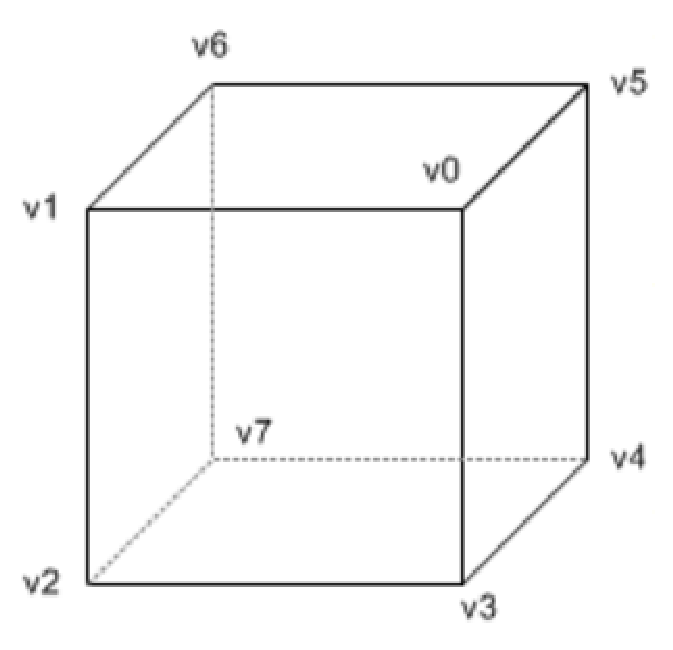
\includegraphics[height=5cm,
    angle=0]{./images/cube.eps}}
\caption{A cube with 6 vertices}
\label{fig:cube}
\end{figure}


As you can see, in intermediate mode, we need to call functions to set
the data for every vertex. For a geometric shape with thousands of
primitives, a better way is to use Vertex Arrays (read
Sect.~\ref{sec:cuda-app.-with}). 

\begin{framed}
  Note that not all of OpenGL commands can be placed in between
  glBegin() and glEnd(). Only a subset of commands can be used;
  glVertex*(), glColor*(), glNormal*(), glTexCoord*(), glMaterial*(),
  glCallList(), etc.

  To work with Vertex Arrays, OpenGL provides 3 new functions:
  glDrawArrays(), glDrawElements(), and
  glDrawRangeElements(). Although, an even better approach is using
  Vertex Buffer Objects (VBO) or Displayed
  List\footnote{\url{http://www.songho.ca/opengl/gl_displaylist.html}}.  
\end{framed}

Similar to normal I/O, OpenGL commands are not executed
immediately. They are put to the buffer and executed until buffer is
full\footnote{\url{1http://www.songho.ca/opengl/gl_overview.html}}.
\verb!glFlush/glFinish! are two functions we use to flush data in
buffer to terminal.

More advanced and practical examples, please read
Sect.~\ref{sec:example-2} (GLUT/FreeGLUT),
Sect.~\ref{sec:cuda-app.-with} (CUDA-OpenGL).


References:
\begin{enumerate}
\item \url{http://www.seas.upenn.edu/~cis565/fbo.htm}
\item 
\end{enumerate}



\section{Techniques}

Techniques
\begin{enumerate}
  \item Persistent-mapped buffers
  
  faster streaming of dynamic geometry
  
  \item MultiDrawIndirect (MDI)
  
  faster submission of multiple draw calls
  
  \item Packing 2D textures into arrays
  
  texture changes no longer break batches
\end{enumerate}


\import*{../Data_Visualization/}{GLUT.tex}  

\part{Advanced Widget Toolkits}
\chapter{Motif (aka OSF/Motif)}
\label{chap:Motif}
\label{chap:osfmotif}

Motif (sometimes called OSF/Motif) is industry-standard to design 2D interface.
We can combine with OpenGL for writing 3D application in which the 2D Window is
created by either OSF/Motif drawing area widgets or OpenGL-specific drawing area
widgets. The 3D rendering context then can be bind to this window.

{\bf motif} is an industry standard toolkit/library for building GUI application
in X windows system since 1980s. Different implementations of the Motif API include Open
Motif, LessTif. 
\begin{itemize}
  \item Open Motif: royalty-free distribution if the software that use Open Motif is open source
  
  \item LessTif: created when Motif still priprietary with the goal to bring Motif-compatible implementation to LGPL licensed
\end{itemize}
From 2012, Motif is LGPLv2 licensed.

Motif was used to
\begin{itemize}
  \item build the GUI for Common Desktop Environment (CDE) - a desktop environment for Unix and OpenVMS O/S
  
  \url{http://en.wikipedia.org/wiki/Common_Desktop_Environment}
  
  
\end{itemize}  


To download motif: \url{motif.ics.com/motif/downloads}

\section{Versions}


Since Motif 2.1, it supports
\begin{itemize}
  \item Unicode
\end{itemize}


\url{http://bwachter.lart.info/documentation/guitoolkits.html}


Motif allows theme creation, but it is not as easy to do as GTK+ (Chap.\ref{chap:GTK+}). One has to
create a long and complex resources file to change the look and feel of Motif
programs. GTK+ users can have this functionality much more easily.

\section{Motif terms}
\label{sec:Motif_terms}

A shell widget acts as the top-level window of the application and handles the
application's interaction with the window manager

Application context
\begin{verbatim}
XtAppContext     app;
\end{verbatim}
is a structure that Xt uses to manage some internal data associated with an
application. Most often, an application receives an opaque pointer to an application context
in the toolkit initialization call and merely passes that pointer to a few other toolkit functions that require it as an argument. 

Even the application context is not being used in most application, the fact
that the application context is a public variable, rather than hidden in the
toolkit internals, is a forward-looking feature of Xt, designed to support
multiple threads of control.

\section{Xm library}
\label{sec:Xm}

The widget set for Motif is implemented in the Xm library
\begin{verbatim}
-lXm
\end{verbatim}
Xm relies on Xt library (Sect.\ref{sec:Xt}).

The header files in \verb!/usr/Motif2.1/include/Xm!
\begin{verbatim}
#include <X11/Intrinsic.h>
#include <X11/Shell.h>
#include <X11/Xatom.h>
#include <Xm/XmStrDefs.h>
#include <Xm/VirtKeys.h>

#include <Xm/PushB.h>  // PushButton widget
\end{verbatim} 
The one with the name ending in a "P" (e.g. PushBP.h) is the widget's private
header file and should not normally be included directly by an application.
Private header files are generally used only by the code that implements a
widget class and its subclasses.

NOTE: \verb!<Xm/XmAll.h>! header file simply includes all of the public
header files.

\subsection{Localization (internalization)}

\begin{verbatim}
XtSetLanguageProc (NULL, NULL, NULL);
\end{verbatim}
\url{http://www.ist.co.uk/motif/books/vol6A/ch-2.fm.html}

\section{How to write a GUI app}

Before an application creates any widgets, it must initialize the toolkit
\begin{itemize}
  \item \verb!XtVaAppInitialize()! (deprecated)
  \item \verb!XtVaOpenApplication()!
\end{itemize}
Example:
\begin{verbatim}
Widget           toplevel;
XtAppContext     app;
toplevel = XtVaOpenApplication (&app, "Hello", NULL, 0, &argc, argv, NULL,
                                sessionShellWidgetClass, NULL);    
\end{verbatim}
which returns a shell widget (Sect.\ref{sec:Motif_terms})


\section{Compile a Motif-based GUI program}

\begin{verbatim}
cc -O -o filename filename.c -lXm -lXt -lX11
\end{verbatim}
The order is important as Xm relies on Xt, and both Xm and Xt rely on Xlib (the -lX11 link flag specifies
Xlib).


\section{Tutorial}

\url{http://www.ist.co.uk/motif/books/vol6A/ch-2.fm.html}
\chapter{KDE}

\section{Introduction}

At that time, none of the application under Unix dekstop, including the desktop
itself, has a nice interface. Matthias Ettrich want to build not only a set of
applications, but a desktop environment in which users could expect things to
look, feel, and work consistently. Then, he founded KDE project in 1996. KDE
stands for K Desktop Environment, with K = Kool or Common, defined by Matthias
Ettrich. Nowadays, it's considered as the coolest or most widely used
cross-platform desktop environment.

Initially, KDE use Motif graphical widget toolkit to develop interface and
productivity tools. Then, Matthias decided to use Qt library for developing GUI
(Chap.\ref{chap:Qt}) for KDE. To guarantee Qt is availble for free with KDE, KDE
Free Qt foundation was created. [NOTE: As an effort to avoid using commercial
product like Qt, GNOME project was started in 1997]. In 1998, the first KDE/Qt
desktop environment, KDE 1.0, was released, Fig.\ref{fig:kde1}.
Many softwares used KDE have the name with 'K' as prefixes, e.g. Konsole (free
terminal emulator), Kaffeine (a media-player). The core libraries of KDE was
licensed under GNU LGPL; but proprietary software need to follow Qt properietary
license to use KDE.


In 2000, KDE 2.0 was released with major changes: KParts (allow an application
to embed another within itself), KHTML (a HTML rendering engine used by
Konqueror web browser), KIO (I/O library), DCOP (Desktop COmmunication
Protocol).

In 2002, KDE 3.0 Dekstop Environment was released, built upon Qt 3 (released
under LGPL for Linux or Unix-like OS only). To run on Windows, it need KDE on
Cygwin (which is now stopped due to available of KDE 4 fow Windows).

In 2008, KDE 4.0 Dekstop Environment was released based on Qt 4 (released under
LGPL for both Windows and MacOS X).  Since 2009, KDE projects was rebranded,
giving KDE no longer stands for K Desktop Environment, but act as an umbrella
brand for software produced by the community. So, from KDE 4.0, KDE (desktop)
was given the name KDE Software Compilation 4 (KDE SC 4) or {\bf KDE platform
4}. The term doesn't target to any particular KDE product.
So, KDE-based software like Amarok or Digikam, are not part of KDE SC. Also,
since then, no major release of KDE has been announced since the acquisition of
Trolltech (the company manage Qt) by Nokia. Major changes are:
\begin{enumerate}
  \item Kicker (the main panel like Star horizonal bar on Windows) + KDesktop
  (a virtual background window to draw icons or other graphics) +
  SuperKarambar (a tool allowing programmers to create gadgets on KDesktop
  virtual window) $\rightarrow$ they are all replaced by KDE Plasma. There are
  three workspaces: KDE Plasma Desktop, KDE Plasma Netbook and KDE Plasma
  Active (for tablet, phone). 
  
%   4.9 with different layout, e.t.
%   Dolphin
   
\end{enumerate}


Since 2011, CMake was used as the build tool for KDE, giving better support for
a wide range of platform. Roadmap for KDE 5.0 was announced in Aug, 2011
\footnote{\url{http://www.itworld.com/mobile-wireless/191083/kde-50-roadmap-announced}}.
Major changes include focusing on mobile devices

% When KDE and Qt are libraries for developing GUI, a
% common name them is {\it widget toolkit}. Qt can also be used to develop non-GUI
% applications.

\begin{figure}[hbt]
  \centerline{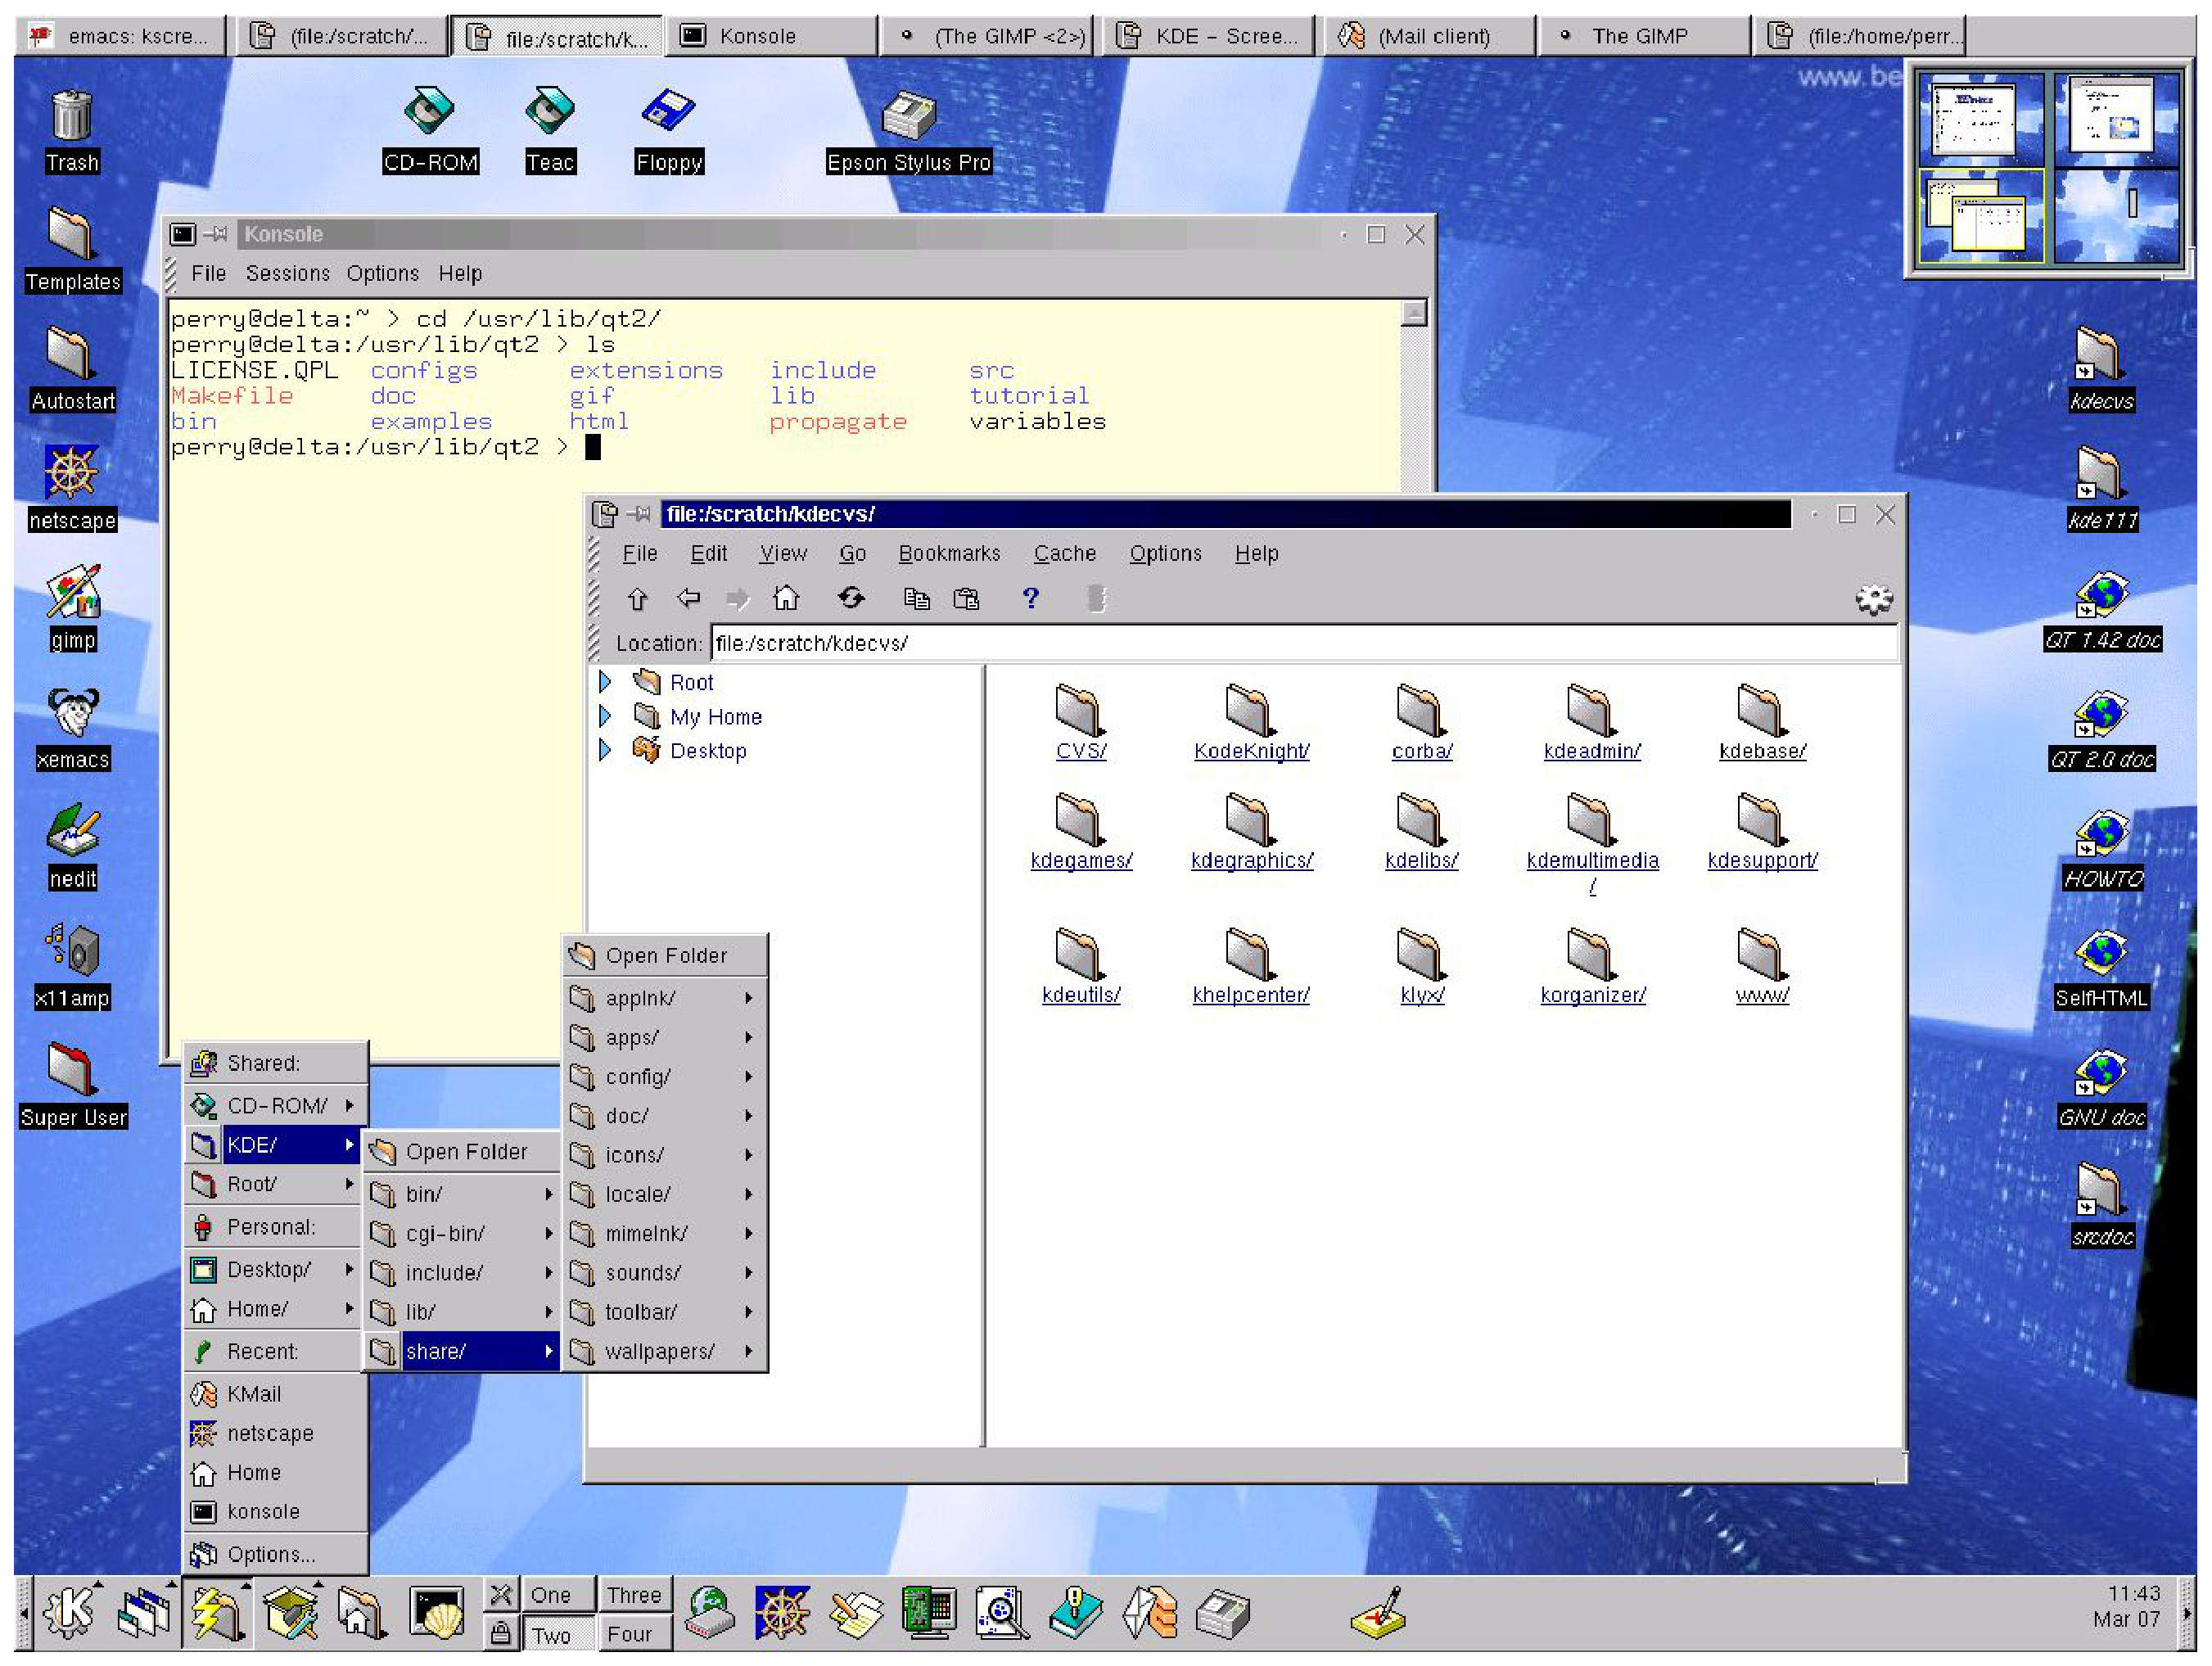
\includegraphics[height=5cm,
    angle=0]{./images/kde1.eps}}
\caption{KDE 1.0 Desktop}
\label{fig:kde1}
\end{figure}


\chapter{GNOME}
\label{sec:GNOME}
\label{chap:GNOME}

GNOME is a desktop environment and GUI that runs on top of an OS. It's free and
an alternate choice to KDE (as KDE use Qt a commercial product). GNOME was
created in 1997, using {\bf GTK+} widget toolkit.  GNOME = GNU Network Object
Model Environment. GTK+ reduces the amount of work when porting one application
to other platforms (Windows, Mac OS X, etc.).


\section{GNOME 1 and GNOME 2}
\label{sec:GNOME-1}
\label{sec:GNOME-2}

GNOME 1 use Nautilus as default file manager (Sect.\ref{sec:nautilus}).
Nautilus is  equivalent to Windows Explorer in Windows.

GNOME 2 use Metacity as default window manager.
Metacity is the Window manager that deals with the behavior of a Window like
maximize, minimize, close, resize, move.

In GNOME 1 and 2, GNOME was designed based on traditional desktop metaphor, i.e.
users can change the looking of the desktop by using different themes (which
usually contains ions, window manager border). 



\section{Cinnamon}
\label{sec:Cinnamon}

Cinnamon is a desktop environment based on GNOME 3 (Sect.\ref{sec:GNOME-3})

As GNOME Shell is far away different from GNOME 2-like user interface, some
efforts have been made to keep GNOME2 layout on top of GNOME Shell. One of that
is {\bf Cinnamon Shell} (Linux Mint distro), which use GNOME Shell (Mutter and
GTK+ 3).

In Cinnamon Shell, window manager is {\bf Muffin}, a fork of Mutter. In Cinnamon
1.6, the default file manager is {\bf Nemo} (not Nautilus).

\section{GNOME 3}
\label{sec:GNOME-3}

Gnome 3 is the third iteration in the Gnome desktop environment. t features a
bar at the top with a clock and a menu button on the left which will bring up a
fullscreen window containing most applications. 

The default theme is rather dark with much black in the general elements, but
the windows are light gray. 


Since GNOME 3, there are many changes that makes it looks similar to Mac OS X
\begin{enumerate}
  \item maximize and minimize button are no longer on the title bar (default)
  
  \item Mutter replaces Metacity as window manager. Mutter is a {\it
  compositing window manager} which allows rendering layout better and faster.
  
  \item GNOME Shell - Sect.\ref{sec:GNOME-Shell} (only works with Mutter)
  replaces GNOME Panel.
  
\end{enumerate}
% Since GNOME 3, it uses {\bf GNOME Shell} (rather than traditional desktop
% metaphor like Nautilus or Metacity) - Sect.\ref{sec:GNOME-Shell}.

\subsection{GNOME Desktop}
\label{sec:GNOME-desktop}

GNOME Desktop on the other hand has lot more than GNOME Shell
(Sect.\ref{sec:GNOME-Shell}). Think of GNOME Desktop as a super set of GNOME
shell; by having also various Gnome specific applications, packages along with
gnome-session.

Example: to install GNOME Desktop, you also need to choose the display manager
(Sect.\ref{sec:Display_manager}), e.g. LightDM - Sect.\ref{sec:LightDM}.

\begin{verbatim}
// OPTION 1
sudo apt-get install ubuntu-gnome-desktop
// and choose lightdm
// during the installation
// Ubuntu comes with LightDM as default display manager

// OPTION 2
// to keep GUI minimal
// will skip extra tools and apps and will install only basic desktop
// environment with few supported tools
sudo apt-get install --no-install-recommends ubuntu-desktop
\end{verbatim}


NOTE: \verb!ubuntu-gnome-desktop! install a full GNOME desktop environment
(including gnome-shell), along with a few standard applications and
optimizations for Ubuntu. Check dependencies
\begin{verbatim}
apt-cache depends ubuntu-gnome-desktop | grep gnome-shell
\end{verbatim}


\subsection{GNOME Shell (2011+)}
\label{sec:GNOME-Shell}

GNOME Shell is simply a desktop environment which changes the user interface.
I would suggest to install GNOME Shell. It will give you a feel of GNOME and you
can easily remove it as well.

GNOME Shell provides a graphical shell and is a more abstract metaphor where
switching between different tasks and virtual workspaces takes place in a
separate area called Overview.

\verb!gnome-shell! will only install the GNOME shell, and its dependencies. In
contrast to \verb!ubuntu-gnome-desktop! (Sect.\ref{sec:GNOME-desktop}), it won't
install the package gnome-session (among others) automatically, which you need
to actually use the GNOME desktop.
\begin{verbatim}
sudo apt-get install gnome-shell

//remove
sudo apt-get remove gnome-shell
\end{verbatim}
GNOME Shell is written in C and JavaScript as a plugin for Mutter.
\url{https://en.wikipedia.org/wiki/GNOME_Shell}


\subsection{Gnome 3.10 with Ubuntu 14.04}
\label{sec:GNOME-3.10}

In an earlier message by Sebastien Bacher's (software engineer at Canonical)
that GTK 3.10 deprecates several options, and thus Ubuntu 14.04 LTS decided to
use Gnome 3.8
\url{http://www.webupd8.org/2013/10/ubuntu-1404-lts-to-stay-on-gtkgnome-38.html}

Later on, however, Ubuntu 14.04 uses GTK 3.10
\url{http://www.webupd8.org/2013/12/gtk-310-lands-in-ubuntu-1404-trusty-tahr.html}
\url{http://www.webupd8.org/2014/01/gnome-shell-310-lands-in-ubuntu-1404.html}

GNOME 3.10 has
\begin{enumerate}
  \item  initial Wayland support, 
  
  \item header bars (client side decorations): it uses the GTK+ toolkit and
  theme engine
  
  \item a new  system menu for GNOME Shell which combines the previous system status menus
  and of course, updated core GNOME apps as well as some new applications.  

  the old system status menus have been replaced with a new System Menu: 

  \item new core apps: 
  Bijiben, a note taking app, GNOME Weather and GNOME photos
  
  \item change in existing core apps:
  
\begin{verbatim}
Web: DuckDuck go is now the default search engine; Web now has a search provider
for GNOME Shell which allows accessing your web history or searching the web
from the GNOME Shell Activities  

Contacts: UI enhancements, updated setup and accounts dialogs

Tweak Tool: redesigned for GNOME 3.10 and includes new options, such as startup
applications management, etc.  

Evince Document Viewer: improved accessibility, new Caret Navigation mode,
improved Djvu support and a new sidebar showing search results  

Clocks: Pretty new analog timer in stopwatch and timer views as well as
geolocation support 

Boxes: support for importing system images (QEMU, raw, vdi - Virtualbox 1.1
image format, vmdk - VMware 3 and 4, vpc and cloop) as well as many UI and other fixes 
\end{verbatim}
  
\end{enumerate}
\url{http://www.webupd8.org/2013/09/see-whats-new-in-gnome-310-video.html}

\subsection{Gnome 3.12+ issues with Ubuntu 14.04}
\label{sec:GNOME-3.12}

Ubuntu 14.04 uses Gnome 3.10.  However, after Gnome 3.10, e.g. Gnome 3.12+,
there happened huge differences on Gnome side, it's not compatible with current
Ubuntu. Even compiz won't work properly. Ubuntu team patches Gnome to use it.
\url{https://askubuntu.com/questions/497955/how-do-you-update-gtk-and-or-gnome-on-ubuntu-14-04-lts}

If you want to upgrade, follow the steps
\url{https://wiki.ubuntu.com/UbuntuGNOME/HowTo/UpgradeGnomeShell}

\url{https://launchpad.net/~gnome3-team/+archive/ubuntu/gnome3-staging/+index?batch=75&direction=backwards&memo=225&start=150}
\begin{verbatim}
// GNOME 3.12 in Ubuntu 14.04

//remove first
ppa-purge gnome3-team/gnome3-staging
ppa-purge gnome3-team/gnome3

// then
sudo add-apt-repository ppa:gnome3-team/gnome3-staging
sudo add-apt-repository ppa:gnome3-team/gnome3
sudo apt-get update

  // if already have GNOME
  // also choose a Display Manager, e.g. GDM or LightDM
sudo apt dist-upgrade
 // if not, install GNOME
sudo apt-get install gnome gnome-shell
\end{verbatim}

If you're going GNOME-only then GDM is fine. But if you plan to switch between
GNOME and other DEs I recommend sticking with LightDM.


GNOME 3.12 has
\begin{enumerate}
  \item full Wayland support - Sect.\ref{sec:Wayland},
  
  \item introduce a Sound Recorder preview release, 
  
  \item Systemd for the user session, 
  
  \item colour tinting in GNOME Shell, 
  
  \item videos application implementation, support for Facebook in GNOME photos,
  integrate Zimbra in GNOME, Git integration in the developer experience as well
  as ratings, screenshots and history support in GNOME Software.
\end{enumerate}


\chapter{Ubuntu}

Ubuntu is based on Debian distro (Sect.\ref{sec:Debian}).

\section{Debian vs. Ubuntu}
\label{sec:Debian}

Check Debian version in Ubuntu
\begin{verbatim}
cat /etc/debian_version
\end{verbatim}
\url{https://askubuntu.com/questions/445487/what-debian-version-are-the-different-ubuntu-versions-based-on}

\subsection{Debian vs. Ubuntu versions}
\label{sec:Debian-versions}

The following lines give a mapping from Ubuntu version to Debian version.

sid is the development distribution of Debian (sid - testing - stable)
\begin{verbatim}
18.04  bionic     buster  / sid
17.10  artful     stretch / sid
17.04  zesty      stretch / sid
16.10  yakkety    stretch / sid
16.04  xenial     stretch / sid
15.10  wily       jessie  / sid
15.04  vivid      jessie  / sid
14.10  utopic     jessie  / sid
14.04  trusty     jessie  / sid
13.10  saucy      wheezy  / sid
13.04  raring     wheezy  / sid
12.10  quantal    wheezy  / sid
12.04  precise    wheezy  / sid
11.10  oneiric    wheezy  / sid
11.04  natty      squeeze / sid
10.10  maverick   squeeze / sid
10.04  lucid      squeeze / sid
\end{verbatim}

Ubuntu is often ahead of Debian on core packages like libc6. Trying to install a
package built on Ubuntu on a contemporary version of Debian is likely to end up
with version errors on libc6.

% Debian version on which your Ubuntu version is based in the file:
% \verb!/etc/debian_version!

% \begin{verbatim}
% 17.10  artful     stretch / sid
% 17.04  zesty      stretch / sid
% 16.10  yakkety    stretch / sid
% 16.04  xenial     stretch / sid
% 15.10  wily       jessie  / sid
% 15.04  vivid      jessie  / sid
% 14.10  utopic     jessie  / sid
% 14.04  trusty     jessie  / sid
% 13.10  saucy      wheezy  / sid
% 13.04  raring     wheezy  / sid
% 12.10  quantal    wheezy  / sid
% 12.04  precise    wheezy  / sid
% 11.10  oneiric    wheezy  / sid
% 11.04  natty      squeeze / sid
% 10.10  maverick   squeeze / sid
% 10.04  lucid      squeeze / sid
% \end{verbatim}
% NOTE: sid is the development distribution of Debian (sid - testing - stable)

% Debian version
% \begin{verbatim}
% Debian 9 (stretch)
% 
% Debian 8 (jessie) 
% 
% Debian 7 (wheezy) 
% \end{verbatim}
\url{https://www.debian.org/releases/}

\subsection{Debian 9 (stretch)}
\label{sec:Debian-stretch}

Uses
\begin{verbatim}
Linux kernel 4.9 LTS
apt 1.4.6
gcc 6.3

libc version 2.24-11

Gnome 3.22 
KDE Plasma 5.8 LTS
Xfce 4.12

Database: MariaDB 10.1 (a MySQL variant)
      to replace MySQL 5.5 or 5.6

systemd version 232  
\end{verbatim}

\url{https://www.debian.org/News/2017/20170617}
\section{debuild vs. dpkg-buildpackage}
\label{sec:dkpg-buildpackage}

debuild and dpkg-buildpackage initialize the environment variable  CFLAGS to a
certain value.

\subsection{clean code for clean build}

As the \verb!debian/rules! file actually calls a Makefile, then this Makefile
should have a \verb!clean! target:
\begin{verbatim}
make clean
\end{verbatim}

or
\begin{verbatim}
dpkg-buildpackage -rfakeroot -Tclean
\end{verbatim}

\subsection{debuild}
\label{sec:debuild}

debuild is a convenient wrapper around dpkg-buildpackage, fakeroot, lintian, and
debsign. It handles all the packaging linting, and signing for us.

debuild will make use of symlinks in it's build process, so if you are using a
Virtualbox or VMware Shared folder to build your package, it will not work.

NOTE: debuild and dpkg-buildpackage initialize the environment variable  CFLAGS to a
certain value.

REQUIREMENTS:
\begin{enumerate}
  \item a \verb!debian/! folder
  
  where all of our debian specific packaging files will go.
  
  \item a \verb!debian/control! file
  
  Example: it describes your package using debian control fields. 
  \begin{verbatim}
  Source: helloworld  
Maintainer: Julio Capote <julio@packagecloud.io>
Build-Depends: debhelper (>= 8.0.0)
Standards-Version: 3.9.3
Section: utils

Package: helloworld  
Priority: extra  
Architecture: any
Depends: ${shlibs:Depends}, ${misc:Depends}  
Description: a simple helloworld package
 Just prints "Hi", it's very useful.
  \end{verbatim}
  
  \item a \verb!debian/changelog! file
  
  This file tracks all the changes to the package. You need a minimum of one
  entry to build a package.
  
  The syntax of this file is tricky, and it is recommended to use
  \verb!debchange! utility (or dch) to create this file.
  \begin{verbatim}
  dch -i -create
  \end{verbatim}
  
  Make sure you change UNRELEASED to unstable
  
  \item a \verb!debian/rules! file
  
  This file tells debian specifically how to build your package. The most basic
    implementation just passes all calls to the original Makefile
   
\begin{verbatim}
#!/usr/bin/make -f  
%:  
	dh $@
\end{verbatim} 
    
    \item a \verb!debian/copyright! file
    
 It can be empty
 \begin{verbatim}
 Copyright 2015, Computology LLC.
 \end{verbatim}
\end{enumerate}




\chapter{Clutter}
\label{chap:Clutter}

Mutter is extensible with plugins and supports numerous visual effects. 

\part{GUI Prototype}
\chapter{Blend for Visual Studio 2012+}
\label{chap:Blend_VisualStudio}

{\bf Microsoft Blend for Visual Studio} (formerly Microsoft Expression Blend
\footnote{It was one of the applications in the Microsoft Expression Studio
suite before that suite was discontinued.
\url{https://www.microsoft.com/expression/eng/}}) helps you design and build
engaging and sophisticated user interfaces by providing you with an accurate
design surface and tools that let you visually create and edit Microsoft Windows
applications.

It is an interactive, WYSIWYG front-end for designing XAML-based interfaces for
Windows Presentation Foundation (WPF) and Silverlight applications.

It can be used to build
\begin{itemize}
  \item Windows Store app
  
  \item Window Phone apps
  
  \item SketchFlow prototype

Tutorial:
\url{http://h20564.www2.hp.com/hpsc/swd/public/readIndex?sp4ts.oid=5060943&swLangOid=8&swEnvOid=4059}
  
  \item WPF 
  
  \item Silverlight
\end{itemize}


\url{https://msdn.microsoft.com/en-us/library/jj171012(v=vs.110).aspx}

\section{SketchFlow (prototype)}
\label{sec:SketchFlow}

With SketchFlow, a designer can quickly and easily create an interactive map
that represents the flow of an application.
It contains a number of {\it screens} - a virtual whiteboard
 on which you can scribble, draw, write, or insert any of the existing user
interface (UI) modeling features of Blend to build a UI. You can also use
screens to create reusable elements such as logos, backgrounds, or UI templates,
and then include those screens as elements in other screens.


\url{https://msdn.microsoft.com/en-us/library/jj969614(v=vs.110).aspx}

\part{Graph Layout}
\chapter{Library for Graph Layout}


\section{GraphViz}
\label{sec:GraphViz}


\subsection{PyGraphViz (Python)}
\label{sec:PyGraphViz}

PyGraphviz is a Python interface to the Graphviz graph layout and visualization
package. With PyGraphviz you can create, edit, read, write, and draw graphs
using Python to access the Graphviz graph data structure and layout algorithms.
\url{https://pygraphviz.github.io/}





\part{C/C++ binding}
\chapter{Qt}
\label{chap:Qt}

\section{History of Qt}

Developing a cross-platform GUI application was unavailable at that time.
Haavard started developing C++ GUI framework since 1988. In summer 1990, Haavard
Nord and Eirik Chambe-Eng were working together on developing GUI for a C++
database application for ultrasound images. The application should be able to
run with a GUI on different platforms:
Unix, Macintosh and Windows. They came up with an object-oriented display
system, or a object-oriented cross-platform GUI
framework\footnote{\url{http://www.civilnet.cn/book/embedded/GUI/Qt4/pref04.html}}.
In 1991, Haavard started writing classes and collaborated with Eirik on the
design. In 1992, Eirik came up with a simple but powerful GUI programming
paradigm {\bf ``signals and slots''} (Sect.\ref{sec:signal_and_slot}) and
Haavard hand-coded it. In 1993, they completed their Qt's first graphics kernel,
which allows them to build their own widgets. 'Q' was chosen as the classes
prefixes because the letter tool beautiful in Haavard's Emacs font, and 't' =
toolkit (inspired by Xt or X toolkit).

In 1994, the company was first established under the name {\it Quasar
Technologies}, and then renamed as Trolltech; with Haavard Nord (Trolltech's
CEO) and Eirik Chambe-Eng (Trolltech's president). The first public release was
Qt 0.90 on May, 1995. \textcolor{red}{Qt offered the same APIs on both Windows
and Linux}.

KDE project was established in 1996 by Matthias Ettrich who decided to use Qt to
build KDE helped Qt became the de-facto standard in C++ GUI development on
Linux. Matthias joined Trolltech in 1998. Qt 2.0 was released in 1999 with a new
open-source license.

By the end 2000, Trolltech released {\bf Qtopia Core}, a platform for
applications to run on embedded devices with its own windows system as a
replacement for X11. Also, the UNIX version of Qt was made available under GPU
LGPL.

Qt 3.0 was released in 2001, with support for Windows, Mac OS X, Unix and Linux
(desktop and embedded), giving 42 different classes. \textcolor{red}{New
features are Unicode support and improved locale, a Perl-like regular expression
class, new text viewing and editing widget}.

Qt 4.0 was released in 2005, with about \textcolor{red}{500 classes, more than
9000 functions}.
Due to its large size and wide-range of features, it was splitted into different
libraries so that developers need only to link to what they need. The major
changes are: completely new set of efficient and easy-to-use template
containers, advanced model/view, fast and flexible 2D painting framework,
powerful Unicode text viewing and editing classes. For the first time, Qt have
two versions: commercial and open-source development on all platforms that it
supports.

In 2008, Trolltech was then acquired by Nokia with the new name Qt Software, and
Qtopia was renamed to {\bf Qt Extended}, targeting to commercial support.  An
agreement between Nokia and KDE in that Nokia is obliged to continue the
development of Qt and provide it as free
software\footnote{\url{http://www.itworld.com/mobile-wireless/289651/alternate-history-kde}}.
In 2009, Qt Software was renamed to Qt Development Framework; and Qt Extended
was discontinued with latest version 4.4.3. The open-source community took it
over with the new name {\bf Qt Extended Improved}, with latest version 4.5.2 in
June 2009.

Since Qt 4.5, Qt was made available under LGPL version 2.1 license, making it
available for commercial products to use the open-source version of Qt. In 2011,
Qt Development Framework was then sold to Digia PLC.
In Sep 2012, the latest stable release was Qt 4.8.3; and Qt 5.0 beta was
released on Aug, 2012; and Qt 5.0 final to be released on Nov 2012. Qt 5.0
offers full capability of OpenGL/OpenGL ES graphics acceleration.


\section{Qt 5}

On a VNC session, we can test if Qt5 is working by running
\begin{verbatim}
python3

>>> from PyQt5 import QtWidgets
>>> qapp = QtWidgets.QApplication([''])


QXcbConnection: Failed to initialize XRandr
Qt: XKEYBOARD extension not present on the X server.
\end{verbatim}
Xrandr - Sect.\ref{sec:Xrandr}

\subsection{Xrandr}
\label{sec:Xrandr}

\begin{verbatim}
typedef struct {
     int type;               /* event base */
     unsigned long serial;   /* # of last request processed by server */
     Bool send_event;        /* true if this came from a SendEvent request */
     Display *display;              /* Display the event was read from */
     Window window;          /* window which selected for this event */
     int subtype;            /* RRNotify_ subtype */
} XRRNotifyEvent;
\end{verbatim}



\url{https://sourcecodebrowser.com/libxrandr/1.2.3/_xrandr_8h_source.html}

\subsection{EGLFS}
\label{sec:EGLFS}

Since the Qt 5.0 release, Qt no longer contains its own window system (QWS)
implementation. There are multiple platform plugins that are potentially usable
on Embedded Linux systems: EGLFS, LinuxFB, KMS, DirectFB, Wayland. 

EGLFS is a platform plugin for running Qt5 applications on top of EGL and OpenGL
ES 2.0 without an actual windowing system (like X11 or Wayland)

\subsection{Troubleshoot: cross-compile}

\begin{verbatim}
./configure -release -opengl es2 -device linux-rasp-pi2-g++ -device-option
CROSS_COMPILE=$TOOLCHAIN/arm-bcm2708/gcc-linaro-arm-linux-gnueabihf-raspbian/bin/arm-linux-gnueabihf- -sysroot $ROOTFS -prefix /usr/local/qt5
\end{verbatim}


\subsection{Troubleshoot: QXcbConnection, XKEYBOARD}

On Linux, the xcb QPA (Qt Platform Abstraction) platform plugin is used. It
provides the basic functionality needed by Qt GUI and Qt Widgets to run against
X11. It seems that vncserver (which is also a trimmed version of X11
server) doesn't provide many of the X extensions in the free version.

\begin{itemize}
  \item  Qt5.6:\url{http://doc.qt.io/qt-5.6/linux-requirements.html}

  \item Latest Qt 5.9: \url{http://doc.qt.io/qt-5/linux-requirements.html}
\end{itemize}

It's best to compile Qt yourself, using \verb!-qt-xcb! so that it statiscally
link against these X11 extension library instead of trying to link against
the system versions.  This can help make Qt less dependent on some of the xcb
helper libraries that might not be available on all distributions. On Ubuntu,
install these packages
\begin{verbatim}
sudo apt-get install libfontconfig1-dev libfreetype6-dev libx11-dev \
libxext-dev libxfixes-dev libxi-dev libxrender-dev \
libxcb1-dev libx11-xcb-dev libxcb-glx0-dev
\end{verbatim}
Build option \url{http://doc.qt.io/qt-5/configure-options.html}
\begin{verbatim}
./configure --prefix=/packages/qt/5.6 -qt-xcb -qt-zlib -qt-libjpeg -qt-libpng
-qt-xkbcommon -qt-freetype -qt-pcre -qt-harfbuzz
\end{verbatim}


Check the output of the command:
\begin{verbatim}
xprop -root | grep -i xkb

// on Mac
_XKB_RULES_NAMES(STRING) = "base", "empty", "empty", "", ""

// on Linux
CUT_BUFFER0(STRING) = "xprop -root | grep -i xkb "
\end{verbatim}

There are several ways how Qt can obtain a keymap information from the X server,
I would recommend to compile Qt applications with xcb-xkb support,
\begin{verbatim}
1) use xkb_x11_* API (from libxkbcommon)
2) if Qt is compiled with Xlib support then use Xlib + xkbfile calls
3) read _XKB_RULES_NAMES property
\end{verbatim}

Check xrandr
\begin{verbatim}
xrandr -q

 SZ:    Pixels          Physical       Refresh
*0   1800 x 1024   ( 457mm x 260mm )  *60  
Current rotation - normal
Current reflection - none
Rotations possible - normal 
Reflections possible - none
\end{verbatim}

\subsection{Qt 5.6}


\url{https://download.qt.io/archive/qt/5.6/5.6.0/}


\section{signal and slot}
\label{sec:signal_and_slot}

Qt defines an extension to C++ language and thus need to be handled by a special
compiler called {\bf MOC} (Meta-Object Compiler- Sect.\ref{sec:MOC}).

\url{http://qt-project.org/doc/qt-4.8/signalsandslots.html}


Slots are just regular methods. Nothing special there, EXCEPT moc will save
their signature in a table in the intermediate .moc file - you can see this
table quite clearly when you look through this file.

This table allows you to call a method using it's signature.

The SLOT(mySlot(int)) macro boils down to a string representation of the method
in question. There are several ways you can do this, see the documentation for
QMetaObject for example.

When a you connect a signal to a slot, the signal and slot signatures are stored
for later use. When a signal is emitted, all the slots previously connected to
that signal are called using the method described above.

There are 2 types of connection there. First one: slots are called at the time
signal was emitted. And the second one: slots calls are placed in event loop
queue. You can manually select the method in connect, but connecting signal and
slots from different threads are always queued


\section{MOC (Meta-Object Compiler)}
\label{sec:MOC}

Meta-Object Compiler (MOC) handles Qt's C++ extension.
It reads Qt codes and convert the Qt's macros in C++ header file to C++ source
file containing the meta-object code for these classes. The source file
extension is \verb!*.moc!

Qt codes extensively use macros like \verb!Q_OBJECT!.
Qt creates "meta object code" based on "annotations" in your c++ code (eg
\verb!Q_PROPERTY!, \verb!Q_SLOTS! etc).


\url{http://qt-project.org/doc/qt-4.8/moc.html}

\subsection{Meta-object code}

Meta objects enhance programming languages by creating new or manipulate
existing objects. They provide functionalities a language does not actually have
by itself.

The Meta Objects are interpreted either by compile time or run time. In Qt and
C++ it is done during compile time by the Meta Object Compiler (moc) -
Sect.\ref{sec:MOC}). An example case is the usage of the signal/slot concept
(Sect.\ref{sec:signal_and_slot}).


\chapter{GTK+}
\label{chap:GTK+}

\section{GIMP (GTK)}
\label{sec:GTK}

GIMP is released under LGPLv3 and GPLv3+. GIMP is an open-source raster image
editor: image retouching, editing, free-form drawing, resizing, cropping,
photo-montages, converting between different image formats, etc.

The GUI tookit for GIMP is called GTK ({\bf GIMP ToolKit}), which was developed
in parallel to facilitate the development of GIMP software.

Since GIMP 0.6, GTK was designed to replace Motif GUI toolkit
(Chap.\ref{chap:Motif}), i.e. giving prettier look. Since GIMP 0.99, GTK+ was
used (Sect.\ref{sec:GTK+}).

Applications that use GTK: OpenOffice, Firefox, Gaim, GIMP.

There are different wrappers
\begin{enumerate}
  \item GTKmm - Sect.\ref{sec:GTKmm}
  \item GTK+ - Sect.\ref{sec:GTK+}
  \item GTK\# - Sect.\ref{chap:GTKsharp}
\end{enumerate}

\section{GTKmm}
\label{sec:GTKmm}

GTKmm is the C++ wrapper for GTK (Sect.\ref{sec:GTK}).

\section{GTK+}
\label{sec:GTK+}

GTK+ was designed to replace GTK (Sect.\ref{sec:GTK}) in GIMP 0.99.
Cario is a 2D graphic library (Sect.\ref{sec:cairo}), and GTK+ uses it to render
widgets. Cario is low-level.

In the future, it's entirely possible that GTK+ will use Clutter
(Sect.\ref{sec:Clutter}) internally as the base for its widgets - though that's
still a work in progress.
\begin{verbatim}
  GPU <- [ [ Cogl + Cairo ] <- [ GDK + Clutter ] <- GTK+ ] <- application
\end{verbatim}
\url{https://lwn.net/Articles/608501/}

\begin{mdframed}

If you are an app developer you might use GTK+ to create the window, menus,
toolbars, etc and use clutter to draw any app content that is "drawing area
like" and doesn't fit into the widget-based app metaphor. Within Clutter, you
may dig down to Cairo for specific drawing tasks.

\end{mdframed}

GTK+ was designed using object-oriented programming approach based on the
base object called GObject (Sect.\ref{sec:GObject}).

Compared to Motif, GTK+ has a much more advanced object system than Motif. This
is a strong point for GTK+ that make it easier to program.
Another advantage of GTK+ compared to Motif is that GTK+ can easily change
themes. That is, one can devise different look and feels for a GTK+ program by
just changing simple configurations.

GTK+ integrates better with other libraries written for UNIX. Due to its modular
nature, GTK+ can be updated more easily.
\url{http://in4mationflow.com/Prog/Gtk/Gtk-in-Comparison-with-Motif} 

\subsection{check version}

\begin{verbatim}
dpkg -l libgtk* | grep -e '^i' | grep -e 'libgtk-*[0-9]'

apt-cache policy libgtk2.0-0 libgtk-3-0 
\end{verbatim}
list all the libgtk packages, including -dev ones, that are on your system.

Check GTK+ 1.x
\begin{verbatim}
pkg-config --modversion gtk+
\end{verbatim}


Check GTK+ 2.x
\begin{verbatim}
pkg-config --modversion gtk+-2.0
\end{verbatim}

Check GTK+ 3.x
\begin{verbatim}
pkg-config --modversion gtk+-3.0
\end{verbatim}
\url{http://stackoverflow.com/questions/126141/how-do-you-find-out-which-version-of-gtk-is-installed-on-ubuntu}



\subsection{install}

You can run GTK+ apps on KDE (just like you can run Qt apps under Gnome) as long
as you have the appropriate libraries installed. Gnome is the desktop
"environment" and a development platform, individual applications can use
whatever toolkit they like (though it's true that using GTK+ makes interaction
with other Gnome applications easier).

However, some GTK+ apps use components/utilities from the GNOME desktop
environment. To get your GTK+ app to run, you may have to install components
from GNOME. It is recommended to install GNOME
Shell (Sect.\ref{sec:GNOME-Shell}).
\url{https://stackoverflow.com/questions/3339828/is-it-possible-to-run-gtk-apps-without-gnome-or-the-likes}


GTK+3.12 comes with Gnome3.12 (Sect.\ref{sec:GNOME-3.12}). To install GTK+3.12
on Ubuntu 14.04
\url{http://www.webupd8.org/2014/05/how-to-install-gnome-312-in-ubuntu.html}


To install the latest version of GTK+
\begin{verbatim}
sudo add-apt-repository ppa:gnome3-team/gnome3
sudo add-apt-repository ppa:gnome3-team/gnome3-staging
\end{verbatim}

 \subsection{GTK+ 2.0}
 
 \subsection{-- GTK+ 2.8}
 \label{sec:GTK+-2.8}
 
GTK+ 2.8 (2005) began the transition to using Cairo (Sect.\ref{sec:cairo}) to
render the majority of its graphical control elements.
 
 \subsection{GTK+ 3.0}

Since GTK+ 3.0 (2005), all graphical control elements are rendered using
Cairo (Sect.\ref{sec:cairo}).
 
GTK+ 3.13.3 contains 203 active and 37 deprecated widgets.

\subsection{Popover widget}
\label{sec:Popover-widget}

Popover was a new widget added in 3.12, which is what gotk3 currently targets
with the default build


\chapter{wxWidgets}
\label{chap:wxWidgets}

{\bf wxWidgets} toolkit (w = Windows, x = X) was created in 1992 as a C++
library, the time when there is no cross-platform open-source widget toolkit
available.
 
\begin{itemize}
  \item to run on Windows, it was first built on top of MFC (Sect.\ref{sec:MFC})
  
Later on, the Windows port was rewritten using native Windows API.
  
  \item to run on Linux, it was first built on top of XView (Sect.\ref{sec:XView})
  
As XView was later abandoned, wxWidgets was rebuilt on top of Motif
(Chap.\ref{chap:Motif}).

In 1995, a Linux port using X toolkit (Sect.\ref{sec:X_toolkit}) was released so
that wxWidgets can run without Motif as Motif was a commercial product at that
time.
  
  \item there is a port using GTK+ (Sect.\ref{sec:GTK+}) called \verb!wxGTK! (Sect.\ref{sec:wxGTk})
  
  \item to run on Linux-based embedded devices, there is a port using DirectFB (Sect.\ref{sec:DirectFB}) called
  \verb!wxDFB! since wxWidgets 3.0 
  
  
\end{itemize}


\url{https://www.wxwidgets.org/about/history/}

\section{wxWidgets}
\label{sec:wxWidgets}

wxWidgets is cross-platform GUI toolkit (LGPL licensed), with binding for Python
(wxPython - Chap.\ref{chap:wxPython}), Perl (wxPerl - Chap.\ref{chap:wxPerl}),
PHP, Java, Lua, Lisp, Erlang, Eiffel, C\#, BASIC, Ruby and Javascript.

% Why not using wxWidgets?
% \begin{itemize}
%   \item Still provide ANSI and Unicode options
%   \item the IDE for wxWidgets is Dev-C++ which has no support for code completion, code generation \ldots 
%   
%   \item wxWidgets does not have an official GUI designer like QT does, however.
%   
%   \item no proxy support in the socket library
%   \item not good documentation
%   \item the design is based on Dev-C++ (a not good IDE)
% \end{itemize}
%   
% Why wxWidgets?
% \begin{itemize}
%   \item cross-platforms
% \end{itemize}

\subsection{Install on Ubuntu}
\label{sec:wxWidgets-install}

\url{http://linuxg.net/how-to-install-wxwidgets-3-0-2-on-ubuntu-14-04-linux-mint-17-elementary-os-0-3-deepin-2014-and-other-ubuntu-14-04-derivatives/}
{\tiny
\begin{verbatim}
sudo apt-key adv --fetch-keys http://repos.codelite.org/CodeLite.asc

sudo apt-add-repository 'deb http://repos.codelite.org/wx3.0.2/ubuntu/ trusty universe'

sudo apt-get update

sudo apt-get install libwxbase3.0-0-unofficial libwxbase3.0-dev libwxgtk3.0-0-unofficial libwxgtk3.0-dev wx3.0-headers wx-common
\end{verbatim}
}


\subsection{Versions 2.x}

As wxWidgets was made to help users that were using MFC to migrate easier, it
inherited a lot of bad things from MFC.

wxWidgets 2.8.6: two separate builds (Unicode \verb!wchar_t*! and ANSI \verb!char*!)

\subsection{Version 3.x}

wxWidgets 3.0 beta: only one build, support Unicode but also support \verb!char *! and
simply convert them using the current encoding transparently.

New classes
\begin{enumerate}
  \item \verb!wxDataViewCtrl! : to replace \verb!wxListCtrl!
\end{enumerate}

Improvements:
\begin{enumerate}
  \item wxFileCtrl 
  \item wxGTK: with wxToolBar, wxStaticText, wxHyperlinkCtrl
  
\end{enumerate}

New features in existing classes
\begin{itemize}
  \item auto-completion: wxTextCtrl and wxComboBox.
\end{itemize}

\url{http://wxwidgets.blogspot.com/2007/11/looking-forward-to-wxwidgets-3.html}

\section{Important classes}

Important classes in wxWidgets toolkit
\begin{enumerate}
  \item \verb!wxSizer! : Sizers are classes derived from the abstract 
  base \verb!wzSizer! class, Fig.\ref{fig:wxSizer_class}
  
\begin{verbatim}
#include <wx/sizer.h>
\end{verbatim}  
  It is a method of choice to define the layout of a control (subwindow) in dialogs (window), 
  as their ability to create a visually appealing
  dialogs independent of the platforms, taking into account the differences in size and 
  style of the individual UI controls.
  
  \url{http://docs.wxwidgets.org/trunk/overview_sizer.html}
  
  The layout algorithm used by sizers in wxWidgets is closely related to layout
  systems in other GUI toolkits, such as Java's AWT, the GTK toolkit or the Qt
  toolkit.
  The idea is that individual subwindows reporting their minimal required size
  and their ability to get stretched if the size of the parent window has
  changed.
\url{http://docs.wxwidgets.org/trunk/classwx_sizer.html}

\begin{figure}[hbt]
  \centerline{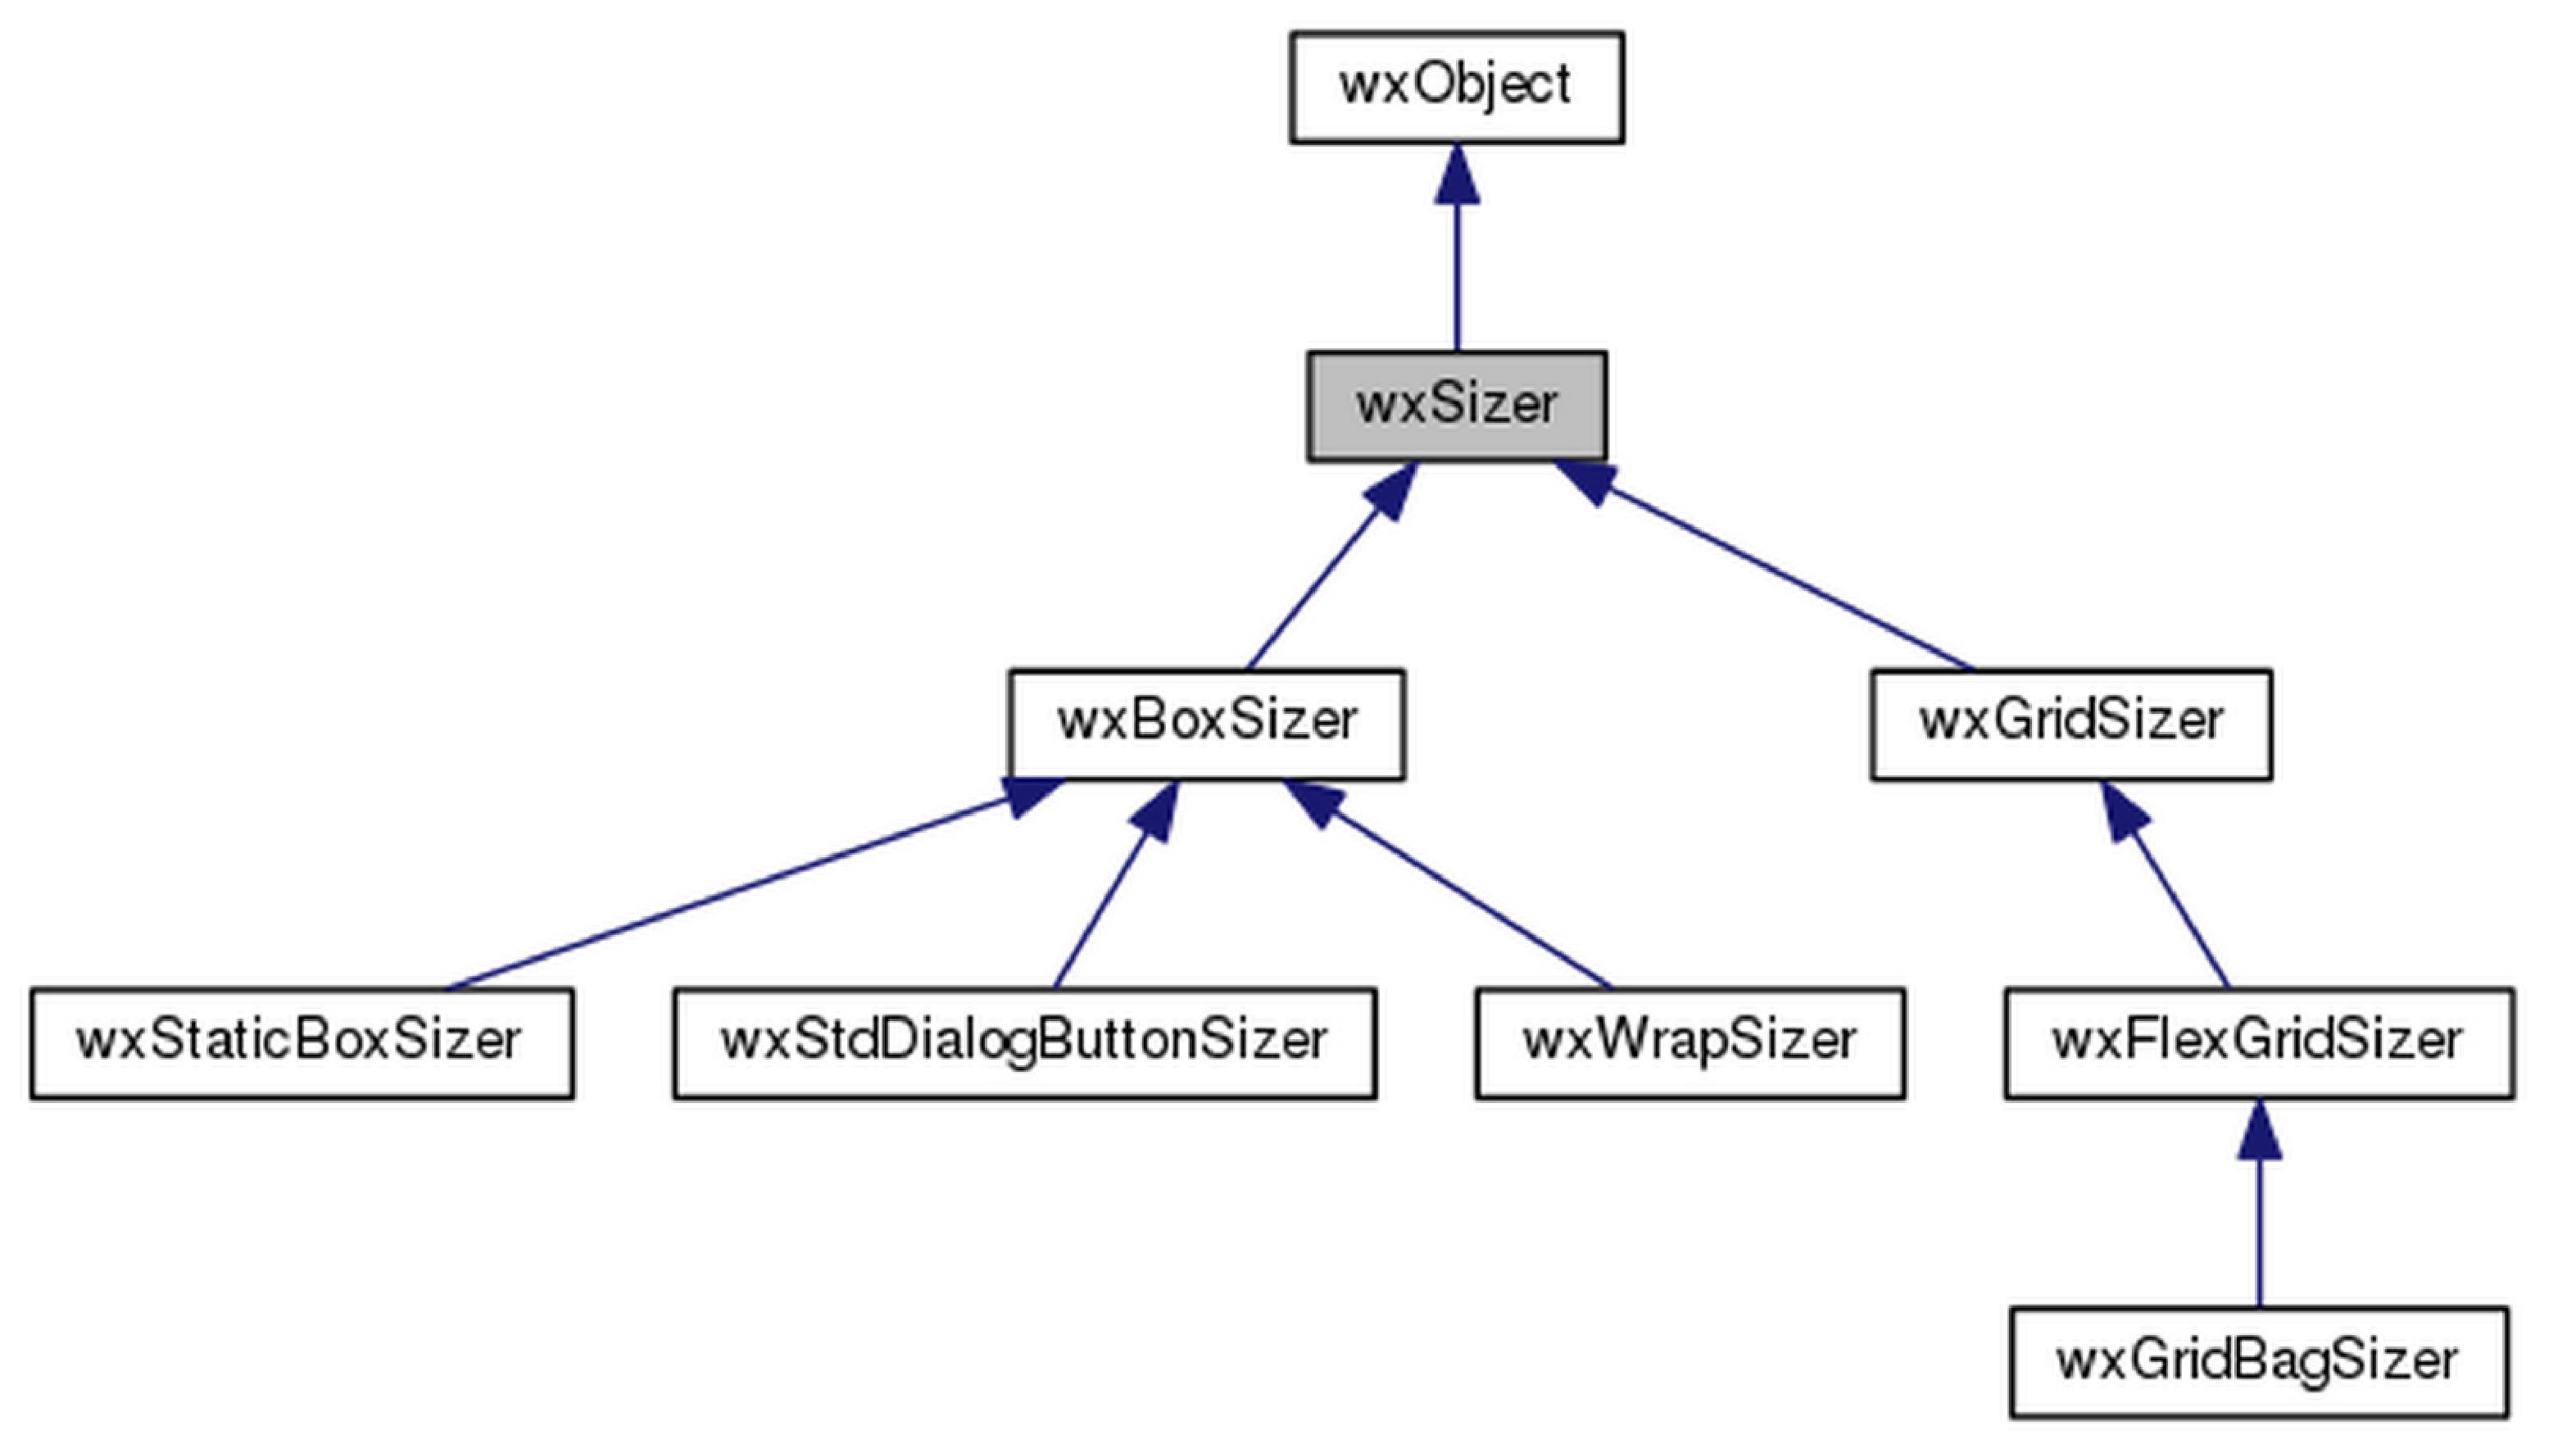
\includegraphics[height=5cm,
    angle=0]{./images/wxSizer_class.eps}}
\caption{wxSizer class hierarchy}
\label{fig:wxSizer_class}
\end{figure}  
  
  
  \item \verb!wxWindow! : a generic class for any drawable object on the screen
  
  \url{http://docs.wxwidgets.org/trunk/classwx_window.html}
  
  \item \verb!wxFrame! (to-level window): A frame is a window whose size and
  position can (usually) be changed by the user, Fig.\ref{fig:wxFrame_class}
  
\begin{verbatim}
#include <wx/frame.h>
\end{verbatim}

It usually has thick borders and a title bar, and can optionally contain a menu
bar, toolbar and status bar. A frame can contain any window that is not a frame
or dialog. 
  
\begin{figure}[hbt]
  \centerline{
\includegraphics[height=5cm,
    angle=0]{./images/wxFrame_class.eps}}
\caption{wxFrame class hierarchy}
\label{fig:wxFrame_class}
\end{figure}  

REMARKS: An application should normally define an wxCloseEvent handler for the
frame to respond to system close events, for example so that related data and
subwindows can be cleaned up.
\url{http://docs.wxwidgets.org/trunk/classwx_frame.html}
    
  \item \verb!wxDialog! : a window for short-term interaction with users to query some information.
  
From the programmer perspective: a dialog does not delete itself after close, so
the information from it can be retrieved it is closed. Thus \verb!wxDialog!
class is often used for preferences dialog (as in web browser) or font dialog
(as in Word processor).

  \item \verb!wxPanel! : a subclass of \verb!wxWindow!. It is a window on which GUI controls are placed.
  
 It is usually placed within a frame (wxFrame).

To have TAB traversal in the frame, we need to use \verb!wxControlContainer! class.
\url{http://docs.wxwidgets.org/trunk/classwx_panel.html}
\begin{verbatim}
#include <wx/containr.h>

#include <wx/panel.h> 
\end{verbatim}

\end{enumerate}


Example: application design: under normal circumstances, you create a frame (subclass of wxFrame),
place a panel in the frame, then place other wxWindow subclasses (wxButton,
wxTextCtrl, etc.) in the panel.



\url{https://wiki.wxwidgets.org/WxFAQ}

\url{https://wiki.wxwidgets.org/Guides_&_Tutorials}


\subsection{wxSizer class}

{\bf wx.BoxSizer} class: and its children
\begin{verbatim}
 wxStaticBoxSizer
 wxStdDialogButtonSizer
 wxWrapSizer
\end{verbatim}

A wx.BoxSizer will lay out its items in a simple row or column, depending on the
orientation parameter passed to the constructor.

It can grow in both directions (height and width) but can distribute its growth
in the main direction (horizontal for a row) unevenly among its children.
 
\url{http://wxpython.org/docs/api/wx.BoxSizer-class.html}




\section{wxGTK library}
\label{sec:wxGTk}

The reason for the existence for wxGTK is to provide a port to using GTK+ via wxWidget. 

However, as there is no static library in GTK+, we can only build linking to GTK+ shared library.

\url{http://stackoverflow.com/questions/1875855/statically-linking-gtk-libaries-in-windows}

\url{https://www.wxwidgets.org/docs/faq/gtk/}

\section{How to write a GUI application with wxWidget?}

A wxWidget application (GUI and console) has no \verb!main()! procedure, 
the reason is that it's not a universal entry point, e.g in Windows \verb!WinMain()! is used.
So, wxWidgets uses the macro \verb!IMPLEMENT_APP(<GUI class>)! as the entry
point, to hide the complexity behind O/S. The equivalent is
\verb!wxApp::OnInit()! member defined in the class derived from \verb!wxApp!.


We need to create an instance of \verb!wxApp! class for a \verb!wxWidget!-based application, 
and implement \verb!__init__! method of this derived class.
If we need the GUI part, inside this method we need to create an instance of
\verb!wxFrame! class, and enable it to show up.

\url{https://wiki.wxwidgets.org/Development:_wxWiki_Documentation_Example}

So for a wxWidget-based GUI application, you need (1) define a subclass of
\verb!wxApp!, (3) call \verb!IMPLEMENT_APP! macro on this derived class, and (3)
implement the \verb!OnInit()! member function of this derived class (with the
minimal implementation is to create a top window) in which we need to create an instance of
\verb!wxFrame! or its derived class.

\begin{verbatim}
#include "wx/wx.h"  // global include

class DerivedApp : public wxApp
{
public:
    virtual bool OnInit();
    
    // define UI controls
    wxCHMHelpController *m_helpCtrl;
};

IMPLEMENT_APP(DerivedApp)

bool DerivedApp::OnInit()
{
  // create the frame, or any UI controls
  
    wxFrame *the_frame = new wxFrame(NULL, ID_MYFRAME, argv[0]);
    ...
    
  // show the frame
    the_frame->Show(true);
    
    // tell which one is the top window
    SetTopWindow(the_frame);

    return true;
}

int MyApp::OnExit()
{
    delete m_helpCtrl;
    return 0;
}
\end{verbatim}
\url{http://packages.das-netzwerkteam.de/doc/wxPython-2.9.1.1/overview_app.html}

Example: define your own frame class, so that you can put more UI controls on it
(Sect.\ref{sec:add_UI_components_to_wxWidget_GUI_Frame})
\begin{verbatim}
class MyFrame: public wxFrame
{
public:
  MyFrame(const wxString& title, const wxPoint& pos, 
                                  const wxSize& size);

  void OnQuit(wxCommandEvent& event);
  void OnAbout(wxCommandEvent& event);

private:
  DECLARE_EVENT_TABLE()
};


\end{verbatim}

\subsection{Building GUI using GUI builder/editor}

To help building the UI faster, we can use widgets Editor for \verb!wxWidgets!
\begin{itemize}
  \item wxWidgets Dialog Editor
  \item wxDesigner
  \item DialogBlocks
  \item XRCed
  \item wxWorkshop
\end{itemize}

\subsection{Working with GUI in multi-threaded application}

wxWidgets (like most GUI toolkits underneath it) is not thread-safe, and
handling of GUI components should always be done exclusively in the main thread.
So your threads must not edit the GUI controls directly, but post an event to
the main thread and let it do the job, i.e.
event passing between thread remains the correct way to go.

\begin{verbatim}
#include <wx/thread.h>
\end{verbatim}

NOTE:  ::wxMutexGuiEnter and ::wxMutexGuiLeave serves as a hack to do the job, but is not recommended.

To send the message, in the form of {\bf custom event}, to the main thread, we follow
\url{https://wiki.wxwidgets.org/Inter-Thread_and_Inter-Process_communication#Sending_custom_events_to_the_main_thread}

\url{http://www.codeproject.com/Articles/11515/Introduction-to-wxWidgets}


\section{How to add menu to Frame}

Define an instance of \verb!wxMenuBar! class. 

To add one or more menu items, define instances of \verb!wxMenu! class
\begin{verbatim}
 menubar = new wxMenuBar;
 file = new wxMenu;
 menubar->Append(file, wxT("&File"));
\end{verbatim}

Finally, set the menu to this instance of \verb!wxMenuBar!
\begin{verbatim}
 SetMenuBar(menubar);
\end{verbatim}

Example: complete

\begin{verbatim}
// absolute.h
#include <wx/wx.h>

class Absolute : public wxFrame
{
public:
  Absolute(const wxString& title);

  wxMenuBar *menubar;
  wxMenu *file;
  wxMenu *edit;
  wxMenu *help;
  wxTextCtrl *textctrl;

};
\end{verbatim}

In the constructor, create the instances of the menu items and assign the text strings
\begin{verbatim}
// absolute.cpp

#include "absolute.h"

Absolute::Absolute(const wxString& title)
       : wxFrame(NULL, -1, title, wxPoint(-1, -1), wxSize(250, 180))
{
 
 wxPanel *panel = new wxPanel(this, -1);

 menubar = new wxMenuBar;
 file = new wxMenu;
 edit = new wxMenu;
 help = new wxMenu;

 menubar->Append(file, wxT("&File"));
 menubar->Append(edit, wxT("&Edit"));
 menubar->Append(help, wxT("&Help"));
 SetMenuBar(menubar);

 textctrl = new wxTextCtrl(panel, -1, wxT(""), wxPoint(-1, -1),
     wxSize(250, 150));

 Centre();
}
\end{verbatim}

Main app
\begin{verbatim}
// main.h
#include <wx/wx.h>

class MyApp : public wxApp
{
  public:
    virtual bool OnInit();
};

// main.cpp
#include "main.h"
#include "absolute.h"

IMPLEMENT_APP(MyApp)

bool MyApp::OnInit()
{

    Absolute *absolute = new Absolute(wxT("Absolute"));
    absolute->Show(true);

    return true;
}
\end{verbatim}

\section{How to add UI components into a Frame}
\label{sec:add_UI_components_to_wxWidget_GUI_Frame}


\section{How to add plots and charts on a GUI application}


There are many add-ons for wxWidgets toolkit 
\begin{itemize}
\item wx"Pl"Plot (another page about this one)
\item wxPlotCtrl (scroll down)
\item wxMathPlot
\item wxChart
\item wxFreeChart
\item gpPanel (another link)
\item wxArt2D
\end{itemize}
\url{https://wiki.wxwidgets.org/WxFAQ#What.27s_the_difference_between_a_wxFrame_and_a_wxWindow.3F} 

\section{How to create a diagram with connected nodes, e.g. a workflow}?

Even though \verb!wxPanel! class is a window on which other UI controls are put on, it is not a good idea 
to create a \verb!wxPanel! for each node.

There are some tools built as an add-on to \verb!wxWidgets!.
The UI controls can be used to help developping workflow workspace,
Fig.\ref{fig:wxShapeFramework_example}

\begin{itemize}
  \item \verb!wxShapeFramework!
  \item \verb!wxWorkspaceView!: tested on wxWidgets 2.8.0 only
  \url{https://code.google.com/p/wxworkspaceview/}
  
  \item \verb!wxArt2D!
\end{itemize}



\begin{figure}[hbt]
  \centerline{\includegraphics[height=5cm,
    angle=0]{./images/wxShapeFramework_example.eps}}
\caption{Examples of GUI applications created using wxShapeFramework}
\label{fig:wxShapeFramework_example}
\end{figure}


\section{How to connect to database}

There is a class called \verb!wxODBC! that helps connecting to different database tools
\begin{verbatim}
  DB2
  DBASE (III, IV)
  Firebird
  Informix
  Interbase
  MaxDB (from MySQL)
  MS Access
  MS SQLServer
  MySQL
  Oracle (7, 8, 9 are tested)
  PervasiveSQL,
  PostgreSQL
  Sybase Adaptive Server Anywhere
  Sybase Adaptive Server Enterprise
  Virtuoso
  XBASE Sequiter
\end{verbatim}
However, \verb!wxODBC! is removed from wxWidgets 2.8.0 and older as no one is maintaining wxODBC.
\url{https://wiki.wxwidgets.org/ODBC}

We can use different database library for database connection. 
\begin{itemize}
  \item SOCI
  
SOCI is a database access library for C++ that makes the illusion of embedding SQL queries in the regular C++ code, staying entirely within the Standard C++.
\url{http://soci.sourceforge.net/}

  \item SQLAPI++:  C++ library for accessing multiple SQL databases (Oracle, SQL Server, DB2, Sybase, Informix, InterBase, SQLBase, MySQL, PostgreSQL, SQLite, SQL Anywhere and ODBC)
  
\url{http://www.sqlapi.com/}

  \item OTL (Oracle and Odbc Template Library):
  
  \url{http://otl.sourceforge.net/} 
\end{itemize}


\section{UI component classes}

\subsection{label}

\verb!wxStaticText! class
\begin{verbatim}

\end{verbatim}

\subsection{generic textbox input}

A text control allows text to be displayed and edited.
The common base class is \verb!wxTextEntry! 
\begin{itemize}
  \item wxTextCtrl: single or multiple-line (with scrollbar)
  
allow text coloring with \verb!wxTE_RICH2! style  
  
  \item wxComboBox: single-line 
  
  \item wxMaskedEditCtrl: limit certain kind of input
  
  \item wxFormatValidator: limit certain kind of input, good for writing localized numbers
\end{itemize}

\url{https://wiki.wxwidgets.org/WxTextCtrl}

\subsection{time  input}

\verb!wxTimePickerCtrl! class allows user to select time. 

\url{http://docs.wxwidgets.org/trunk/classwx_time_picker_ctrl.html}

\subsection{date input}

\verb!wxDatePickerCtrl! class allows user to select date.

\section{Other add-ons libraries}


\begin{verbatim}
wxMozilla.
wxIndustrialControls.
wxCURL.
ToasterBox.
wxVTK.
wxDockIt.
wxIFM.
wxMathPlot.
wxTreeMultiCtrl.
wxAUI.
wxPropertyGrid.
wxSMTP.
wxResizeableControl.
wxOTL.
wxReportWriter.
wxHyperlinkCtrl.
wxSQLite.
wxIE.
wxCTB.
AWX.
wxSpellChecker.
wxArt2D.
wxImprola.
wxHTML.
wxStEdit.
wxLCDWindow.
mmwx.
LitWindow.
Keybinder.
wxBetterDialog.
wxBZipStream.
wxCrashReport.
wxHTTPServer.
wxRarInputStream.
wxSheet.
wxStreamMerger.
\end{verbatim}
\url{http://www.codeproject.com/Articles/11515/Introduction-to-wxWidgets}
\import*{../C-Cpp_Manual/}{Vala.tex}
\import*{../C-Cpp_Manual/}{GObject.tex}


\part{Python binding}
\import*{../Python_Manual/}{UI_Python.tex}
\import*{../Python_Manual/}{wxPython.tex}
\import*{../Python_Manual/}{turtle_screen}
\import*{../Python_Manual/}{PyQt}

\part{Java binding}
\import*{../Java_Manual/}{Writing_UI_Java.tex}
\import*{../Java_Manual/}{AWT.tex}
\import*{../Java_Manual/}{Swing.tex}
\import*{../Java_Manual/}{JavaFX.tex} 


\part{.NET platform}
\chapter{GTK\#}
\label{chap:GTKsharp}


GTK\# is a Graphical User Interface Toolkit for mono and .Net.
GTK\# is a .NET binding for the GTK+ toolkit. The GTK+ toolkit
(Chap.\ref{chap:GTK+}) is written in C for speed and compatibility, while the
GTK\# binding provides an easy to use, object oriented API for managed use. 

In general, GTK\# applications are written using MonoDevelop, which provides a
visual designer for creating GTK\# GUIs.

Platforms: Unix, Windows, OSX.

\url{http://www.mono-project.com/docs/gui/gtksharp/}


\chapter{MonoMac}
\label{chap:MonoMac}

MonoMac is aimed at .Net/Mono developers that want to allow their users to have
a native Mac OS X application experience. MonoMac allows developers to access
the whole range of MacOS X APIs from C\#, it is not limited to the AppKit GUI APIs.  

The MonoMac APIs replaced the old CocoaSharp binding, which is now deprecated.

Platforms: OSX
\chapter{Windows.Forms}
\label{chap:Windows.Forms}

Platforms: Windows, Unix, OSX.

Microsoft's \verb!System.Windows.Forms! (aka Managed.Windows.Forms, MWF,
Winforms) is a binding developed by Microsoft to the Win32 toolkit. It is 
 a popular toolkit used by millions of Windows developers (especially for
internal enterprise applications).

The Mono project decided to produce a compatible implementation (Winforms) to
allow these developers to easily port their applications to run on Linux and other Mono platforms.   
Mono's System.Windows.Forms ({\bf MWF}) is implemented using
\verb!System.Drawing!.
All controls are natively drawn through System.Drawing.
System.Windows.Forms implements its own driver interface to communicate with the
host OS windowing system. The available driver interfaces supports X11, Win32,
OSX.

Most of the Windows.Forms API will work on Mono, however some applications (and
especially third party controls) occasionally bypass the API and P/Invoke
straight to the Win32 API. These calls will likely have to changed to work on
Mono.  

In general, Winforms applications are written using Microsoft's Visual Studio or
SharpDevelop, which both provide a visual designer for creating Winforms GUIs.
As WinForms is designed for Desktop-based applications; many people are shifting
to using WPF which is designed to be both Desktop-based and Web-based friendly
(Chap.\ref{chap:WPF}). However, at the moment, WinForms has more supported GUI
elements; while with WPF you may need to buy third-party packages.

\section{Windows Form with C++/CLI}

Before Visual Studio 2012
\begin{verbatim}
File/New/Project...
    Visual C++ (project types)
       CLR
          Windows Forms Application (Templates)
\end{verbatim}

According to the VC++ team, the primary intent of C++/CLI was to provide for
great interop solutions, and not another full-featured .NET language. So if
you're looking to build a new .NET based desktop apps, C\# or VB.NET are the
recommended choices going forward.  So, since Visual Studio 2012, this feature
is removed from the Wizzard.
\url{https://social.msdn.microsoft.com/Forums/vstudio/en-US/2acadc0f-33b6-43e2-aff7-52654cc48ab8/how-to-create-windows-forms-application-in-vs-c-2013-rc?forum=vcgeneral}

However, we still can create a Winforms application using C++/CLI, from Visual
Studio 2012
\begin{verbatim}
File/New/Project...
    Visual C++ (project types)
       CLR
          CLR Empty Project	
\end{verbatim}
Suppose you name the project is CUDAFLuxGUI.

Then Project/Add New Item\ldots
\begin{verbatim}
Visual C++
   UI
     Windows Form
\end{verbatim}
and create a new form name (e.g. MainForm.h), then edit \verb!MainForm.cpp!. In
the code (NOTE: You can also copy the form designed in C\# project; however
partial class is not supported here).

\begin{verbatim}
#include "MainForm.h"

using namespace System;
using namespace System::Windows::Forms;

[STAThread]
void main(array<String^>^ arg) 
{
   Application::EnableVisualStyles();
   Application::SetCompatibleTextRenderingDefault(false);
   
   //Create the form instance
   CUDAFluxGUI::MainForm form;
   
   Application::Run(%form);

}
\end{verbatim}
The System namespace provides functions to work with UI controls. Then,
right-click on the project, get \verb!Properties! window
\begin{verbatim}
Configuration Properties
    Linker
        System
\end{verbatim}
select  Windows (/SUBSYSTEM:WINDOWS) for SubSystem. If you don't see
\verb!SubSystem!, make sure you change the configuration setting from Win32 to
x64. (See Sect.\ref{sec:configuration-properties_Linker_subsystem} in
Visual C++ chapter in C/C++ manual book)

\begin{verbatim}
Advanced
   Entry point
\end{verbatim}
type in \verb!Main!; then hit OK button. 

IMPORTANT: Make sure the above settings are set for both Debug and Release
configuration.

Finally, hit F5 to test the program.

\url{http://www.bogotobogo.com/cplusplus/application_visual_studio_2013.php}


If you check the \verb!MainForm.h! file, it has
\begin{verbatim}
#pragma once

namespace CUDAFluxGUI {

	using namespace System;
	using namespace System::ComponentModel;
	using namespace System::Collections;
	using namespace System::Windows::Forms;
	using namespace System::Data;
	using namespace System::Drawing;

	/// 

	/// Summary for MyForm
	/// 

	public ref class MainForm : public System::Windows::Forms::Form
	{
	public:
		MainForm(void)
		{
			InitializeComponent();
			//
			//TODO: Add the constructor code here
			//
		}
        ...

\end{verbatim}

Explain:
\begin{itemize}
  \item \verb!#pragma once! : it means only open this file once during the
  compilation. \verb!System! namespace gives us functions to deal with UI
  controls.
  \item a class name \verb!MainFrom! is derived from the Windows Form
  \verb!Form! base class.
\end{itemize}



To deploy the system, create another project 
\begin{verbatim}
Installed
   InstallShielf Limit ... Setup and Deployment
\end{verbatim}
and name it \verb!Setup_CUDAFluxGUI!. From the Project Assistant window, we
setup the properties of the installation. 

\section{Windows Form with .NET language (C\#)}

\section{Form class}
\label{sec:Form-class}

\begin{verbatim}
System.Windows.Forms.Form 
\end{verbatim}
Represents a window or dialog box that makes up an application's user interface.
The main windows of an application is a derivative of this class.

\url{http://msdn.microsoft.com/en-us/library/system.windows.forms.form(v=vs.110).aspx}

\begin{verbatim}
namespace CUDAFluxGUI
{
    public partial class MainForm : Form
    {
    	// (private) data members
    	
    	// constructor
    	public MainForm() : base()
    	{
    	  // do GUI setting
    	  // initialize data members
    	}
    }
}
\end{verbatim}

You have the option to create MDI application (multiple-document interface),
that allows you to open multiple files, and a Windows menu to switching from one
document to another.
\url{http://msdn.microsoft.com/en-us/library/xyhh2e7e(v=vs.110).aspx}

\section{Application class (sealed)}
\label{sec:Winforms.Application}

\begin{verbatim}
System.Windows.Forms.Application
\end{verbatim}
class is an important class, it contains \verb!static! method that can be used
to control the GUI of the application and other tasks (e.g. start/stop the
application).

Example: below is the core functional calls in the Main() method
\begin{verbatim}
using System.Windows.Forms;

public class Form1 : System.Windows.Forms.Form
{

[STAThread]
static void Main() 
{
// the first line in Main() method
   Application.EnableVisualStyles();

// to use GDI based TextRenderer class for text rendering
   Applications.SetCompatibleTextRenderingDefault(false);

// Add the event handler for handling UI thread exceptions to the event.
   Application.ThreadException += new
      ThreadExceptionEventHandler(ErrorHandlerForm.Form1_UIThreadException);
    
    
   Application.Run(new Form1());
}

public Form1()
{
 //UI components here
}
\end{verbatim}
The \verb!Run()! method start the application message loop on the current
thread, and (optionally) make the form visible.
\begin{verbatim}
Application.Run() 	// without a form

Application.Run(new Form1()) // make the form visible
\end{verbatim}

\url{http://msdn.microsoft.com/en-us/library/system.windows.forms.application(v=vs.110).aspx}


\section{Colors}


\begin{verbatim}
System.Drawing.Color class

System.Drawing.SystemColors class
\end{verbatim}

Example:
\begin{verbatim}
Color toolStripMenuItemSelectedColor = Color.FromArgb(194, 224, 255);
Color toolStripMenuItemUnSelectedColor = SystemColors.Control;
\end{verbatim}

\section{Menu}

\begin{verbatim}
System.Windows.Forms.Menu
  System.Windows.Forms.MainMenu  //the class is replaced by 
                                   MenuStrip  (.NET 2.0+)
  
System.Windows.Forms.Menu
  System.Windows.Forms.ContextMenu  // the class is replaced by
                                      ContextMenuStrip (.NET 2.0+)
        
  
System.Windows.Forms.Control
  System.Windows.Forms.ScrollableControl
    System.Windows.Forms.ToolStrip
      System.Windows.Forms.MenuStrip   // represent a menu system for a
                                        Form (or it derivative class)
            

System.Windows.Forms.Control
  System.Windows.Forms.ScrollableControl
    System.Windows.Forms.ToolStrip
      System.Windows.Forms.ToolStripDropDown
        System.Windows.Forms.ToolStripDropDownMenu
          System.Windows.Forms.ContextMenuStrip   // represent a shortcut menu                                   
\end{verbatim}

\section{Menu Item}

\begin{verbatim}
System.Windows.Forms.Menu
  System.Windows.Forms.MenuItem  // a single menu item displayed on
                            MainMenu or ContextMenu 
                           the class is replaced by ToolStripMenuItem


      System.Windows.Forms.ToolStripItem
        System.Windows.Forms.ToolStripDropDownItem
          System.Windows.Forms.ToolStripMenuItem  // a selectable menu item on
                                                    MenuStrip or
                                                    ContextMenuStrip
\end{verbatim}

\section{SplitContainer}

SplitContainer class represents a UI control with two sides, and a movable
splitter, which can be configured horizontal spliter or vertical splitter.


\section{Helloworld app}


The programs has the main file (MainForm.cs) with the minimal included headers
\begin{Verbatim}
using System;
using System.Collections.Generic;
using System.ComponentModel;
using System.Data;
using System.Drawing;
using System.Linq;
using System.Text;
using System.Windows.Forms;
\end{Verbatim}

\begin{mdframed}
This is in Mono

\begin{verbatim}
using System;
using System.Drawing;
using System.Windows.Forms;
\end{verbatim}

\end{mdframed}

Next step: put the main class inside a namespace. The name of the namespace is
typically the name of the application
\begin{Verbatim}
namespace CUDAFluxGUI
{
   //put the main GUI class here (e.g. CUDAFluxGUI class)

}
\end{Verbatim}

The main class is defined here
\begin{enumerate}
  \item it is a partial class of the \verb!Form! class
  (Sect.\ref{sec:Form-class})
  \item A public constructor also need to call the default constructor of
  \verb!Form! class.
  
\begin{Verbatim}
public MainForm()
     : base()
 {
\end{Verbatim}
   and call automatic methods that should not be modified
\begin{verbatim}
     InitializeComponent();
     WindowState = FormWindowState.Maximized;     
}
\end{verbatim}


\end{enumerate}

\begin{Verbatim}
//public partial class HelloWorld : Form
public partial class MainForm : Form
    {
        ///

        /// Main constructor for HelloWorld Form
        /// 


        public HelloWorld()
        {
            // initialize the designer standard components
            InitializeComponent();

            // make sure that this window is maximized
            WindowState = FormWindowState.Maximized;
        }

        ///

        /// Called when the form is first loaded.  Resize the HelloWorldLabel to fit the new form size
        /// 


        ///
Ignored
        ///
Ignored
        private void HelloWorld_Load(object sender, EventArgs e)
        {
            ResizeHelloWorld();
        }

        ///

        /// Called when the form is resized.  Resize the HelloWorldLabel to fit the new form size
        /// 


        ///

        ///

        private void HelloWorld_Resize(object sender, EventArgs e)
        {
            ResizeHelloWorld();
        }

        ///

        /// Resize the Hello World to fill the client area
        /// 


        void ResizeHelloWorld()
        {
            // change the font to match the size of the client area
            HelloWorldLabel.Font = GetBestFontFit(ClientSize, HelloWorldLabel.Font, HelloWorldLabel.Text, ClientSize.Height, 8f); ;

            // center the label
            CenterHelloWorld();
        }

        ///

        /// Center the HelloWorldLabel in the client area of HelloWorld form
        /// 


        void CenterHelloWorld()
        {
            HelloWorldLabel.Location = new Point((ClientSize.Width / 2) - (HelloWorldLabel.Width / 2), (ClientSize.Height / 2) - (HelloWorldLabel.Height / 2));
        }

        ///

        /// Determine the best font match for the size/text.  The result should be between the maximum and minimum height.
        /// The size is the area to fill.  The new font is based on the old font which is passed in.
        /// 


        /// Font
        public static Font GetBestFontFit(Size size, Font currFont, String text, float fontMax, float fontMin)
        {
            float fontPixels = fontMax;
            float minfontPixels = fontMin;

            // find the corresponding font size for the textbox size
            Font font = currFont;

            // make sure that the text is not null or empty before attempting to fit it in the area.
            // if it is null or empty, the current font is used since it does not matter.
            if (!String.IsNullOrEmpty(text))
            {
                Size textsize;

                font = new Font(currFont.FontFamily, fontPixels, currFont.Style, GraphicsUnit.Pixel);

                textsize = TextRenderer.MeasureText(text, font);

                // Check to see if the font fits in the area and if not, find a smaller one
                while ((((textsize.Height) > size.Height) || ((textsize.Width) > size.Width)) && (fontPixels > minfontPixels))
                {
                    // try to speed up the process of finding the right font size by detecting how much it is too big by
                    if (textsize.Height > size.Height)
                    {
                        // reduce the fontPixels based on how far off the font size is
                        fontPixels -= (textsize.Height - size.Height);
                    }
                    else if (textsize.Width > size.Width)
                    {
                        int charPixelWidth = textsize.Width / text.Length;
                        int targetPixelWidth = size.Width / text.Length;

                        // if the characters are too wide, reduce the fontPixels by how different the result is from the desired width
                        if (charPixelWidth > targetPixelWidth)
                        {
                            fontPixels -= (charPixelWidth - targetPixelWidth);
                        }
                        else
                        {
                            fontPixels -= 1.0F;
                        }
                    }
                    else
                    {
                        fontPixels -= 1.0F;
                    }

                    // drop the old one since it did not work
                    font.Dispose();

                    // get a new font based on the smaller font pixels size
                    font = new Font(font.FontFamily, fontPixels, font.Style, GraphicsUnit.Pixel);

                    // recalculate the size based on the new font
                    textsize = TextRenderer.MeasureText(text, font);
                }
            }

            // when all done, return the font to use
            return (font);
        }

    }
}
\end{Verbatim}

\section{UI Data binding}
\label{sec:UI-data-binding-WinForms}

Classically, data binding was used within applications to take advantage of data
stored in databases. Windows Forms data binding allows you to access data from
databases as well as data in other structures, such as arrays and collections
(assuming certain minimum requirements have been met). 

In Windows Forms, you can bind a UI control to a wide variety of structures,
from simple (arrays) to complex (data rows, data views, and so on). As a
minimum, a bindable structure must support the \verb!IList! interface.


 To do a simple data binding, e.g. a column value from a dataset table is
displayed in the Windows Form control, we first need to know which data
source we want to connect
\begin{enumerate}
  \item database: MS SQL Server ( .xsd file - a typed dataset)
  
  \item web service: data and method of a WCF service, WCF Data Services or a
  Web service (the type of the returned objects can be varied)
  
  \item objects: work with data in existing objects (the object can be located
  in the project, or you need a reference (add a reference) to the selected
  object first before it shows up in the wizard)
  
  \item SharePoint: data from a SharePoint site
  
\end{enumerate}

A connection object need to be created for the UI form or
component. In Visual Studio, it is typically created as the result of using a
data wizard (Data Source Configuration Wizard)
\footnote{\url{http://msdn.microsoft.com/en-us/library/w4dd7z6t.aspx}} or
dragging data objects onto the form.

Run Data Source Configuration Wizard using either
\begin{enumerate}
  \item Project / Add New Data Source
  \item Data Source Window choose Add New Data Source
  \item From the property of the bindable controls, select Add New Data Source
  command
\end{enumerate}



Once you added the database/data source, you choose {\bf Database Model} to
generate a dataset or EDM (Entity Data Model)
\begin{enumerate}
  \item ADO.NET: \url{http://msdn.microsoft.com/en-us/library/aa984058.aspx}
   \item ASP.NET : \url{http://msdn.microsoft.com/en-us/library/6759sth4.aspx}
\end{enumerate}

Next, choose your data connection
\begin{itemize}
  \item Choose an existing connection (from the list of connections) or create a
  new one (click {\it New Connection})
  \item Set values in {\it Connection Properties} dialog box
  \item read-only information is displayed in {\it Connection Properties} dialog
  box
\end{itemize}

Finally, save the {\bf Connection String} to the App. Configuration file. Type a
name for the connection or use the provided default name. If the database
connection changes, you can modify the connection string in the application
configuration file instead of editing the source code and recompiling your
application. How to edit a connection string
\url{http://msdn.microsoft.com/en-us/library/ms171887.aspx}

Look at {\bf Data Sources} window, once the datasource is available,
\footnote{\url{http://msdn.microsoft.com/en-us/library/6ckyxa83.aspx}} then you
can create data-bound controls (i.e. a control that bind to data) by dragging
the data source to a design surface
\url{http://msdn.microsoft.com/en-us/library/w4dd7z6t.aspx}

\begin{mdframed}
In some situations, it's convenient to create a connection object without the
assistance of any data design tools. E.g.: to create an ADO.NET
programmatically, see
\url{http://msdn.microsoft.com/en-us/library/32c5dh3b.aspx}
\end{mdframed}

  


\url{http://msdn.microsoft.com/en-us/library/aa984214.aspx}


\section{Text rendering: GDI vs. GDI+}
\label{sec:text_rendering}

Some new UI controls use GDI based \verb!TextRenderer! class to do text
rendering; the old one use GDI+ based \verb!Graphics! class. This is the change
made from .NET Framework 2.0 to resolve problems in performance
and localization in GDI+. GDI calculates character spacing and word wrapping
differently from GDI+, which can cause text for controls that use
\verb!TextRenderer! looks different from text rendered by \verb!Graphics! class.
To resolve this incompatibility, you can set the UseCompatibleTextRendering
property to true.  

In most cases, if your application is not being upgraded from .NET Framework
1.0 or .NET Framework 1.1, it is recommended that you leave
UseCompatibleTextRendering set to the default value of false. 

We use
\begin{verbatim}
using Systems.Windows.Forms;

Application.EnableVisualStyles();
 // to use GDI based TextRenderer class for text rendering
Applications.SetCompatibleTextRenderingDefault(false);


Application.Run(new Form1());
\end{verbatim}
See Sect.\ref{sec:Winforms.Application}

IMPORTANT: You should never call this method if your Windows Forms code is
hosted in another application, such as Internet Explorer. Only call this method
in stand-alone Windows Forms applications. 
\url{http://msdn.microsoft.com/en-us/library/system.windows.forms.application.setcompatibletextrenderingdefault(v=vs.110).aspx}
\chapter{WPF (Windows Presentation Foundation)}
\label{chap:WPF}

\section{Introduction}

Typically, writing a GUI app requires at least two threads, one for handling the
main GUI to prevent inresponsiveness for time-consuming task. This requires the
programmers to deal with threading explicitly.

Typically, WPF applications start with two threads: one for handling rendering
and another for managing the UI.
\begin{enumerate}
  \item {\bf rendering thread}: effectively runs hidden in the background -
  Sect.\ref{sec:rendering-thread}
  
  \item {\bf UI thread}: receives input, handles events, paints the screen, and
  runs application code - Sect.\ref{sec:UI-thread} 

Most WPF-based applications use a single UI thread, but there are still
situations where multiple threads improve user interface (UI) responsiveness or
application performance.


\end{enumerate} 

WPF is the latest Microsoft's approach to GUI framework to be used in .NET
framework. A {\bf GUI framework} provides a framework for programmers to create
an application with a wide range of GUI elements, e.g. label, textboxes, \ldots.
This is considered a newer option compared to WinForms
(Chap.\ref{chap:Windows.Forms}).

WPF use XAML which makes it easy to create and edit the GUI
(Sect.\ref{sec:XAML}), while the code for handling the GUI's event can be
written in any .NET languages. To write UI using WPF, we can use
\begin{itemize}
  \item Microsoft Visual Studio (good for both coding and XAML editing)
  \item Microsoft Expression Bend (for designers, part of Expression Studio),
  with supports for gradients, template editing, animation, etc.
  
  Expression Bend can open solution files created by Microsoft VS
\end{itemize}

\url{https://msdn.microsoft.com/en-us/library/ms741870(v=vs.100).aspx}

\subsection{UI thread}
\label{sec:UI-thread}

There is an object of class {\bf Dispatcher} that provides services for managing
the queue of work items for a thread.
Every UI thread must have at least one Dispatcher, and each Dispatcher can
execute work items in exactly one thread (Sect.\ref{sec:Dispatcher_class}), it
selects on a priority basis and runs each one to completion. 

The trick to building responsive, user-friendly applications is to maximize the
Dispatcher throughput by keeping the work items small, i.e. not taking much
time to complete.  Any perceivable delay between input and response can
frustrate a user.



\subsection{(background) rendering thread}
\label{sec:rendering-thread}

Historically, Windows allows UI elements to be accessed only by the thread that
created them. This means that a background thread in charge of some long-running
task cannot update a text box when it is finished. Windows does this to ensure
the integrity of UI components. WPF has a built-in mutual exclusion mechanism
that enforces this coordination. 

If only one thread can modify the UI, how do background threads interact with
the user? - A background thread can ask the UI thread to perform an operation on
its behalf. It does this by registering a work item with the Dispatcher of the
UI thread. The Dispatcher class provides two methods for registering work items: Invoke and BeginInvoke.
Both methods schedule a delegate for execution (NOTE: a delegate is similar to
a function pointer in C/C++, but it is type-safe, i.e. can be checked by the
compiler - check C\# book on how to create a delegate)
  
\begin{itemize}
  \item Dispatcher.Invoke (delegate): synchronous call - doesn't
  return until the UI thread actually finishes executing the delegate

\begin{lstlisting}
    // Place delegate on the Dispatcher.
    this.Dispatcher.Invoke(DispatcherPriority.Normal,
        new TimerDispatcherDelegate(TimerWorkItem));
\end{lstlisting}    

  \item Dispatcher.BeginInvoke: asynchronous call
\end{itemize}

\url{https://msdn.microsoft.com/en-us/library/system.windows.threading.dispatcher.invoke(v=vs.100).aspx}

\subsection{DispatcherObject}
\label{sec:DispatcherObject_class}

Most classes in WPF derive from DispatcherObject.
At construction, a DispatcherObject object stores a reference to the Dispatcher
object linked to the currently running thread. So

\url{https://msdn.microsoft.com/en-us/library/system.windows.threading.dispatcherobject(v=vs.100).aspx}

\subsection{Dispatcher}
\label{sec:Dispatcher_class}

Once an object Dispatcher is created in a thread, it maintains a prioritized
queue of work item for a specific thread. 

If you attempt to get the CurrentDispatcher for the current thread and a
Dispatcher is not associated with the thread, a Dispatcher will be created. A
Dispatcher is also created when you create a DispatcherObject. If you create a
Dispatcher on a background thread, be sure to shut down the dispatcher before
exiting the thread.

\url{https://msdn.microsoft.com/en-us/library/system.windows.threading.dispatcher(v=vs.100).aspx}

\section{WPF with Visual C++}

To create the user interface in WPF we use Extensible Application Markup
Language (XAML - Sect.\ref{sec:XAML}. It's primary measuring unit is not pixel
based, so applications display at any dpi (Resolution independence using vector graphics).
WPF is using DirectX that can enjoy the benefits of hardware acceleration for
smoother graphics and overall better performance.

\url{http://www.bogotobogo.com/CSharp/csharp_wpf_xaml_netframework.php}

\section{XAML}
\label{sec:XAML}


XAML is XML-based language, whose file is used to describe the GUI structures.
XAML is for designer and thus can be split from the
programming part (C\#, VB.NET, \ldots).
\begin{itemize}
  \item use hardware acceleration for drawing the GUI: better performance
  \item UI works for both Desktop-based and Web-based (using Silverlight/XBAP)
  \item first choice by Microsoft, which is being used in newer Visual Studio
  tools
\end{itemize}

All measures in WPF is based on logical units, not pixels. A logical unit = 1/96
of an inch. So, the size of each components doesn't change when you change the
resolution of your screen. However, you can also easily build a scalable UI
using the vector-based rendering engine.

The UI is separated from the behavior (i.e. how each component reacts when user
clicks/selects). The UI is implemented using XAML (Sect.\ref{sec:XAML}); while
the behavior is implementd using C\# or Visual Basic.

In WPF, we can virtually define any types of controls as
content of another.

Example: put an image into a button to create an image button
\begin{verbatim}
<Button>
    <StackPanel Orientation="Horizontal">
        <Image Source="speaker.png" Stretch="Uniform"/>
        <TextBlock Text="Play Sound" />
    </StackPanel>
</Button>
\end{verbatim}

Example: a simple GUI, with a button and a delegate \verb!StartOrstop()! to
handle mouse-click on the button
\begin{verbatim}
<Window x:Class="SDKSamples.Window1"
    xmlns="http://schemas.microsoft.com/winfx/2006/xaml/presentation"
    xmlns:x="http://schemas.microsoft.com/winfx/2006/xaml"
    Title="Prime Numbers" Width="260" Height="75"
    >
  <StackPanel Orientation="Horizontal" VerticalAlignment="Center" >
    <Button Content="Start"  
            Click="StartOrStop"
            Name="startStopButton"
            Margin="5,0,5,0"
            />
    <TextBlock Margin="10,5,0,0">Biggest Prime Found:</TextBlock>
    <TextBlock Name="bigPrime" Margin="4,5,0,0">3</TextBlock>
  </StackPanel>
</Window>

<Window x:Class="SDKSamples.MainWindow"
    xmlns="http://schemas.microsoft.com/winfx/2006/xaml/presentation"
    xmlns:x="http://schemas.microsoft.com/winfx/2006/xaml"
    Title="Prime Numbers" Width="260" Height="75"
    >
    <StackPanel Orientation="Horizontal" VerticalAlignment="Center" >
        <Button Content="Start"  
            Click="StartOrStop"
            Name="startStopButton"
            Margin="5,0,5,0"
            />
        <TextBlock Margin="10,5,0,0">Biggest Prime Found:</TextBlock>
        <TextBlock Name="bigPrime" Margin="4,5,0,0">3</TextBlock>
    </StackPanel>
</Window>
\end{verbatim}

then in the code, we need to define \verb!Window1! class in the
\verb!SDKSamples! namespace
\begin{lstlisting}
namespace SDKSamples
{
    public partial class Window1 : Window
    {
    	public Window1() : base()
        {
            InitializeComponent();
        }
		private void StartOrStop(object sender, EventArgs e)
        { // Delegate
        }
    }
    
}
\end{lstlisting}
\url{https://msdn.microsoft.com/en-us/library/ms741870(v=vs.100).aspx}

\subsection{Delegate}
\label{sec:Delegate}


\import*{../Csharp_Manual/}{Graphics_NET.tex}

\part{Perl}
\import*{../Perl_manual/}{wxPerl.tex}

\part{Audio/Soud Engine} 
\chapter{Sound Engine}
\label{chap:SoundEngine}


\section{DirectSound}
\label{sec:DirectSound}


DirectSound provides a low-latency interface to sound card drivers written for
Windows 95 through Windows XP and can handle the mixing and recording of
multiple audio streams.

Nowadays, DirectSound means DirectX Audio (Sect.\ref{sec:DirectX_Audio}).

\section{DirectSound3D}
\label{sec:DirectSound3D}

DirectSound3D (DS3D) is an extension to DirectSound (Sect.\ref{sec:DirectSound})
introduced with DirectX 3 in 1996 with the intention to standardize 3D audio in
Windows.


\section{DirectX Audio}
\label{sec:DirectX_Audio}

DirectSound and DirectSound3D (DS3D) were officially merged and given the name
DirectX Audio, however the API is still commonly referred to as DirectSound.

\section{EAX}
\label{sec:EAX}

EAX is an extension to DirectSound and DirectSound3D which provides sound
effects processing to the hardware-accelerated buffers.

\section{Cross-platform Audio Creation Tool system (XACT)}
\label{sec:XACT}



\part{Input Engine}
\chapter{Input Engine}
\label{chap:Input_Engine}

Here, we describe the libraries that help us to collect inputs
from input devices
such as the mouse, keyboard, joystick or other game controllers.

\section{DirectInput}
\label{sec:DirectInput}

It provides a system for action mapping, which allows the user to assign
specific actions within a game to the buttons and axes of the input devices. 

Microsoft recommends that new applications make use of the Windows message loop
for keyboard and mouse input instead of DirectInput, and use XInput for Xbox 360
console (Sect.\ref{sec:XInput}).


DirectInput was added from DirectX 1.0 in 1995 with true support for joystick,
i.e.
mouse and keyboard modules simply provided wrappers to the standard Win32 API.

DirectInput in DirectX 3.0 added support for keyboards and mice; it also
improved joystick support.


DirectInput in DirectX 5.0 (1997) included greatly improved joystick support,
including adding force feedback, increasing the number of buttons (mouse button
from 4 to 8), changing the underlying device-driver model and incorporating a
COM-based API.




\section{XInput}
\label{sec:XInput}

The new input library called XInput is specifically for the Xbox 360 controller.


%\chapter{Sound Engine}
\label{chap:SoundEngine}


\section{DirectSound}
\label{sec:DirectSound}


DirectSound provides a low-latency interface to sound card drivers written for
Windows 95 through Windows XP and can handle the mixing and recording of
multiple audio streams.

Nowadays, DirectSound means DirectX Audio (Sect.\ref{sec:DirectX_Audio}).

\section{DirectSound3D}
\label{sec:DirectSound3D}

DirectSound3D (DS3D) is an extension to DirectSound (Sect.\ref{sec:DirectSound})
introduced with DirectX 3 in 1996 with the intention to standardize 3D audio in
Windows.


\section{DirectX Audio}
\label{sec:DirectX_Audio}

DirectSound and DirectSound3D (DS3D) were officially merged and given the name
DirectX Audio, however the API is still commonly referred to as DirectSound.

\section{EAX}
\label{sec:EAX}

EAX is an extension to DirectSound and DirectSound3D which provides sound
effects processing to the hardware-accelerated buffers.

\section{Cross-platform Audio Creation Tool system (XACT)}
\label{sec:XACT}



\chapter{Multi-language support}

\section{gettext}
\label{sec:gettext}

Download:
 \url{http://ftp.gnu.org/pub/gnu/gettext/gettext-0.19.8.tar.gz}


Gettext is a system for writing multilingual program on Unix-like OS. GNU
gettext is one implementation of {\bf gettext}, released in 1995.
\begin{itemize}
  \item Ubuntu 14.04: gettext 0.18.3
\end{itemize}

In C, the function \verb!gettext()! function; whose aliases is \verb!_!
\begin{verbatim}
printf(gettext("My name is %s.\n"), my_name);
printf(_("My name is %s.\n"), my_name);
\end{verbatim}

For comments, to make it should be translated as well, the comment line starts
with three dashses (///). 

\url{http://en.wikipedia.org/wiki/GNU_gettext}.


\chapter{API documentation}

API documentation is important, as help checking the code easier. One widely
tool is \verb!doxygen!.

\section{Doxygen}

	


\chapter{Operating Systems for Mobile Devices}


\section{Meego (canceled in 2011)}
\label{sec:Meeg}

Meego is a Linux-based free Operating System (OS) for mobile devices. The UI
for Meego was based on Qt. It was canceled in Sep, 2011. A newer choice is {\bf
Tizen} (Sect.\ref{sec:Tizen}).


A group continued the development of Meego under a new name {\bf Mer}
(Sect.\ref{sec:Mer}).

\section{Mer}
\label{sec:Mer}

Mer was a continued development from Meego (Sect.\ref{sec:Meego}).
Devices that use Mer as the operating system:
\begin{enumerate}
  \item Vivaldi: use ARM CPU, with KDE Plasma UI (Plasma Active).
  \item Jolla mobile phone: 
\end{enumerate}

\section{Tizen}
\label{sec:Tizen}

Based on WebOS (Sect.\ref{sec:WebOS}), Tizen is an OS for mobile devices,
including smart TV. Users can use HTML5 to write applications. Tizen development
is driven by Intel and Samsung.

Tizen 1.0 was released in April, 2012. Tizen 2.0 will be released in Dec, 2012.
First devices using Tizen will be released in 2013.

\section{WebOS}
\label{sec:WebOS}


\backmatter 
 
% %\include{glossary}
% %\include{notat}
\printindex %Make an index AUTOMATICALLY

%The style you want to use for references.
% %\bibliographystyle{harvard}
% % amsalpha, decsci, development, unsrtnat
%\bibliographystyle{biophysj}
% Use short or long Journal names
% %\bibliography{../longtitles, ../ref_computational_cb} %The files
%\bibliography{shorttitles,ref_computational_cb}
 
\end{document}
